% !TeX encoding = UTF-8
% Entwurf der Doktorarbeit von Domenik Zimmermann, TU M\"unchen, Grp. Prof. Dr. Auw\"arter 
%%%%%%%%%%%%%%%%%%%%%%%%%%%%%%%%%%%%%%%%%%%%%%%%%%%%%%%
\author{Domenik Matthias Zimmermann}
\title{Molecular adsorption on \textit{h}-BN}
%%%%%%%%%%%%%%%%%%%%%%%%%%%%%%%%%%%%%%%%%%%%%%%%%%%%%%%
% Bilder: AFM/STM 1024x1024 px exportieren, 
%
% Fonts are embedded by default, otherwise check 
% https://tex.stackexchange.com/questions/10391/how-to-embed-fonts-at-compile-time-with-pdflatex
% 
% sudo apt-get install kile texlive-latex-extra texlive-science texlive-bibtex-extra biber
%
% adjust kile tools to call biber %lS instead of bibtex
% for TexStudio the command to call biber is biber %
%
% If errors occure referring to aux files or others:
%	Delete helper files (*.aux) and maybe others!
%
% Use MikTeX version 2.9.6615 or later (check that biber is included)
% Using BiBLaTex, biber as frontend.
% If biber complains (ERROR - Error: Found biblatex control file version 2.6, expected version 3.4.)
% 	Update with your Miktex package manager (mpm_mfc.exe[single user install] or mpm_mfc_admin.exe [all user install])
% no new biblatex version there? Sync database? NO improvement!
%%%%%%%%%%%%%%%%%%%%%%%%%%%%% Setup for document %%%%%%%%%%%%%%%%%%%%%%%%%%%%%%%%%
\documentclass[
%11pt,					% Schriftgröße, 11pt is standart
%a5paper,				% a4paper is standart
twoside,				% Zweiseitig
BCOR=12mm,				% Bindekorrektur inkl. Biegefalz
headings=normal,		% Kleinere Kapitelüberschriften => check preamble
headsepline,			% Enable line to seperate head ...
footsepline,			% ... and foot
plainfootsepline,		% Footseperation line on chapter start
%,draft
]{scrbook}
%%%%%%%%%%%%%%%%%%%%%%%%%%%%% Change Page Geometry %%%%%%%%%%%%%%%%%%%%%%%%%%%%%%
\usepackage[
top=30mm,
bottom=55mm,
inner=30mm,
outer=30mm,
%marginparsep=7mm,
%marginparwidth=48mm,
%paperwidth=210mm,
%paperheight=245mm, 286mm (A4)
]{geometry}
%%%%%%%%%%%%%%%%%%%%%%%%%%%%%%%%%%%%%%%%%%%%%%%%%%%%%%%%%%%%%%%%%%%%%%%%%%%%%%%%%%
\usepackage[utf8]{inputenc}
% when latex complains about unicode char U+2212 is not configured for use in latex use the line below
\DeclareUnicodeCharacter{2212}{-}% support older LaTeX versions
%\usepackage[latin1]{inputenc}
\usepackage[T1]{fontenc}
\usepackage{lmodern}
\usepackage[english]{babel}
\usepackage{csquotes}
\usepackage{amsmath}
\usepackage{textcomp}		%enables \textdegree to use as �
\usepackage{amsfonts}
\usepackage{amssymb}
\usepackage{graphicx}
\usepackage{xhfill}			% provides /hrulefill (disclaimer)
%\usepackage{wasysym}		
\usepackage{braket}		% fur <A|H|B> <A| |A> oder <A>
%\DeclareGraphicsExtensions{.pdf,.png,.jpg}
%%%%%%%%%%%%%%%%%%%%%%%%%%%%%
\usepackage{siunitx}
\DeclareSIUnit\langmuir{L}
%%%%%%%%%%%%%%%%%%%%%%%%%%%%%
\usepackage[hidelinks,breaklinks=true]{hyperref}
%\usepackage{url}
\usepackage[section]{placeins} %definiert \floatbarrier, mit option automatisch bei jeder section
%%%%%%%%%%%%%%%%%%%%%%%%%%%%%%%%%%%%%%%%%%%
\usepackage{subfigure}
\usepackage{wrapfig}
%%%%%%%%%%%%%%%%%%%%%%%%%%%%%%%%%%%%%%%%%%%
\usepackage{caption}
\usepackage{microtype}
%\usepackage{subcaption}
\usepackage{multicol}
\usepackage{multirow}
%%%%%%%%%%%%%%%%%%%%%%%%%%%%
% fuer Stichwortverzeichnis
\usepackage{makeidx}
% Stichwortverzeichnis erstellen
\makeindex
%%%%%%%%%%%%%%%%%%%%%%%%%%%%%%%%%%%%%%%%%%%%%%%%%%%%%%%
\usepackage[style=numeric		% bibliogryphy-styles: alphabetic, numeric, chem-angew, ieee, nature, science
,backend=biber
%,refsection=chapter			% setzt bibliographies nach chaptern getrennt, nach jedem chapter muss ein 
								% printbibliogrphy stehen
]{biblatex} 	
\addbibresource{./bib.bib}  	% relative to root directory (where the file that includes this file is located)! 
								%do NOT OMIT .bib ending

%avoids ugly line breaks within bibligraphy
\addto\bibsetup{\setlength{\emergencystretch}{1.5em}} 	

% Zum Verwalten der Zitate benutze ich Zotero, zum Erzeugen der .bib-Datein f�r Latex wird die Exportfunktion von Zotero benutzt (rechtsklick auf ``Meine Bibliothek'' im linken Reiter: Option Biblatex in die Datei bib-zotero-export.bib aus welcher ich dann die betreffenden Zitate auf Richtigkeit \"uberpr\"ufe und in die bib.bib kopiere.
%%%%%%%%%%%%%%%%%%%%%%%%%%%%%%%%%%%%%%%%%%%%%%%%%%%%%%%
% \usepackage[top=2.5cm,left=2.5cm,right=3.5cm,bottom=3.5cm]{geometry}
%%%%%%%%%%%%%%%%%%%%%%%%%%%%%%%%%%%%%%%%%%%%%%%%%%%%%%%
\usepackage{xcolor}
%%%%%%%%%%%%%%%%%%%%%%%%%%%%%%%%%%%%%%%%%%%%%%%%%%%%%%
%%%%%%%%%%%%%%%%%%%%%%%%%%%%%%%%%%%%%%%%%%%%%%%%%%%%%%
\usepackage[draft=false]{scrlayer-scrpage}		%deaktiviert ruler in der draft version
\pagestyle{scrheadings}
%%%%%%%%%%%%%%%%%%%%%%%%%%%%%%%%%%%%%%%%%%%%%%%%%%%%%%
%%%%%%%%%%%%%%%%% DAUMENKINO Footer %%%%%%%%%%%%%%%%%%
	\usepackage{etex}
	\usepackage{intcalc} 
	\newcommand*{\AnzBilder}{200}		            		%<--Variablen anpassen
\newcommand*{\KinoPfad}{./images/animation/lumo/} 	%<--Variablen anpassen

%%%%Quelltext%%%
\newcommand*{\SafeboxName}{sbKino}

\makeatletter
%Erzeugt neue Saveboxen und füllt sie mit includegraphics-Anweisungen
%Aufruf: \NewSaveBoxes{sbKino}{5}{daumenkino/kino}
\newcommand*{\NewSaveBoxes}[3]{%
	\@tempcnta 1
	\@whilenum \@tempcnta< \numexpr(#2+1) \do{%
		%Savebox anlegen
		\expandafter\newsavebox\csname #1\the\@tempcnta\endcsname
		%Savebox mit Leben füllen
		\expandafter\savebox\csname #1\the\@tempcnta\endcsname{%
			\includegraphics[width=0.5cm]{#3\the\@tempcnta}%
		}%
		\advance\@tempcnta 1
	}%
}

\newcommand*{\bildnr}{\numexpr\intcalcMod{\numexpr\value{page}}{\numexpr\AnzBilder}\relax}
\newcommand*{\lumoseries}{%
	\usebox{\@nameuse{\SafeboxName\the\bildnr}}%
}
\makeatother
\NewSaveBoxes{\SafeboxName}{\AnzBilder}{\KinoPfad}
	%inner side of odd pages
	\lofoot[\lumoseries]{\lumoseries} % Add flicker books to [plain.scrheadins] and {scrheadins}!
	% inner side of even pages	
	\newcommand*{\AnzBilderLogo}{200}		            		%<--Variablen anpassen
\newcommand*{\KinoPfadLogo}{./images/animation/logo/} 	%<--Variablen anpassen
%%%%Quelltext%%%
\newcommand*{\SafeboxNameLogo}{sbKinologo}

\makeatletter
%Erzeugt neue Saveboxen und füllt sie mit includegraphics-Anweisungen
%Aufruf: \NewSaveBoxesLogo{sbKino}{5}{daumenkino/kino}
\newcommand*{\NewSaveBoxesLogo}[3]{%
	\@tempcntb 1
	\@whilenum \@tempcntb< \numexpr(#2+1) \do{%
		%Savebox anlegen
		\expandafter\newsavebox\csname #1\the\@tempcntb\endcsname
		%Savebox mit Leben füllen
		\expandafter\savebox\csname #1\the\@tempcntb\endcsname{%
			\includegraphics[width=0.5cm]{#3\the\@tempcntb}%
		}%
		\advance\@tempcntb 1
	}%
}
%intcalc-version
\newcommand*{\bildnrLogo}{\numexpr\intcalcMod{\numexpr\value{page}}{\numexpr\AnzBilderLogo}\relax}

\newcommand*{\logoseries}{%
	\usebox{\@nameuse{\SafeboxNameLogo\the\bildnrLogo}}%
}
\makeatother
\NewSaveBoxesLogo{\SafeboxNameLogo}{\AnzBilderLogo}{\KinoPfadLogo}
%%%Aufruf%%%%%%%
	\refoot[\logoseries]{\logoseries} % Add flicker books to [plain.scrheadins] and {scrheadins}!
%%%%%%%%%%%%%%%%%%%%%%%%%%%%%%%%%%%%%%%%%%%%%%%%%%%%%%
%%%%%%%%%%%%%%%%%%%%%%%%%%%%%%%%%%%%%%%%%%%%%%%%%%%%%%
% Basic information for cover & title page
\newcommand*{\getUniversity}{Technische Universit\"at M\"unchen}
\newcommand*{\getFaculty}{Department of physics}
\newcommand*{\getFacultyger}{Fakult\"at f\"ur Physik}
\newcommand*{\getTitle}{Molecular adsorption on \textit{h}-BN}
%newcommand*{\getTitleger}{TODO: Titel der Abschlussarbeit}
\newcommand*{\getAuthor}{Domenik Matthias Zimmermann}
\newcommand*{\getDoctype}{Dissertation}
\newcommand*{\getDoctypeger}{Vollst\"andiger Abdruck der von der Fakult\"at für Physik der Technischen Universit\"at M\"unchen zur Erlangung des akademischen Grades eines Doktors der Naturwissenschaften (Dr. rer. nat.) genehmigten Dissertation.}
\newcommand*{\getSupervisor}{Prof.\ Dr.\ Wilhelm Auw\"arter}
\newcommand*{\getChairman}{TODO: Chairman}
\newcommand*{\getFirstExaminer}{TODO: 1. Examiner}
\newcommand*{\getSecondExaminer}{TODO: 2. Examiner}
\newcommand*{\getSubmissionDate}{TODO: Submission date}
\newcommand*{\getSubmissionLocation}{Munich}
\newcommand*{\getDisclaimer}{I assure the single handed composition of this \MakeLowercase{\getDoctype{}} only supported by declared resources.}
% TODO: add custom commands etc.

%%%%%%%%%%%%%%%%%%%%%%%%%%%%%%%%%%%%%%%%%%%%%%%%%%%%%%%%%%%%%%%%%%%%%%%%%%%%%%%%%%%%%%%%%%%%%
% Change \autoref (Figure x.x) to FIGURE x.x

%%%%%%%%%%%%%%%%%%%%%%%%%%%%%%%%%%%%%%%%%%%%%%%%%%%%%%%%%%%%%%%%%%%%%%%%%%%%%%%%%%%%%%%%%%%%%
% Python style for highlighting
% Check https://tex.stackexchange.com/questions/83882/how-to-highlight-python-syntax-in-latex-listings-lstinputlistings-command#83883

% Default fixed font does not support bold face
\DeclareFixedFont{\ttb}{T1}{txtt}{bx}{n}{12} % for bold
\DeclareFixedFont{\ttm}{T1}{txtt}{m}{n}{12}  % for normal

\newcommand\pythonstyle{\lstset{
		language=Python,
		basicstyle=\small,             %\ttm, \tiny \small
		otherkeywords={self},             % Add keywords here
		keywordstyle=\small\color{deepblue},
		emph={MyClass,__init__},          % Custom highlighting
		emphstyle=\small\color{deepred},    % Custom highlighting style
		stringstyle=\color{deepgreen},
		frame=tb,                         % Any extra options here
		showstringspaces=false,           % 
		frame=single,
		numbers = left,
		numbersep=5pt
}}
% Python environment
\lstnewenvironment{python}[1][]
{
	\pythonstyle
	\lstset{#1}
}
{}
% Python for external files
\newcommand\pythonexternal[2][]{{
		\pythonstyle
		\lstinputlisting[#1]{#2}}}
% Python for inline
\newcommand\pythoninline[1]{{\pythonstyle\lstinline!#1!}}
%%%%%%%%%%%%%%%%%%%%%%%%%%%%%%%%%%%%%%%%%%%%%%%%%%%%%%%%%%%%%%%%%%%%%%%%%%%%%%%%%%%%%%%%%%%%%

%%%%%%%%%%%%%%%%%%%% Draft Mode Compilation from command line %%%%%%%%%%%%%%%%%%%%
%%%%%%%%%%%%%%%%%%%% pdflatex "\def\draftmode{1} \input{FILE}"  %%%%%%%%%%%%%%%%%%
%%%%%% TEXSTUDIO %%% pdflatex "\def\draftmode{1} \input{%.tex}" %%%%%%%%%%%%%%%%%%
%%%%%%%%%%%%%%%%%%%%%%%%%%%%%%%%%%%%%%%%%%%%%%%%%%%%%%%%%%%%%%%%%%%%%%%%%%%%%%%%%%
%\def\daumenkino{1}
%%%%%%%%%%%%%%%%%%%%%%%%%%%%%%%%%%%%%%%%%%%%%%%%%%%%%%%%%%%%%%%%%%%%%%%%%%%%%%%%%%
%%%%%%%%%%%%%%%%%%%%%%%%%%%%%%%%%%%%%%%%%%%%%%%%%%%%%%%%%%%%%%%%%%%%%%%%%%%%%%%%%%

\begin{document}
%%%%%%%%%%%%%%%%%%%%%%%%%%%%%%%%%%%%%%%%%%%%%%%%%%%%%%%%%%%%%%%%%%%%%%%%%%%%%%%%%%%%%%%%%%%%%%%%%%%%%
%\renewcommand{\figureautorefname}{\texttt{\figureautorefname}} 

 \begin{titlepage}
% HACK for two-sided documents: ignore binding correction for cover page.
% Adapted from Markus Kohm's KOMA-Script titlepage=firstiscover handling.
% See http://mirrors.ctan.org/macros/latex/contrib/koma-script/scrkernel-title.dtx,
% \maketitle macro.
\oddsidemargin=\evensidemargin\relax
\textwidth=\dimexpr\paperwidth-2\evensidemargin-2in\relax
\hsize=\textwidth\relax
%%
\centering
\vspace{50mm}

\includegraphics[width=40mm]{./includes/logo/tum} \\
\vspace{10mm}
{\Huge\MakeUppercase{\getUniversity{}}} \\
\vspace{15mm}
{\huge\MakeUppercase{\getFaculty{}}} \\
\vspace{20mm}
{\Large \getDoctype{}} \\
\vspace{15mm}
{\huge\bfseries \getTitle{}} \\
\vspace{15mm}
{\LARGE \getAuthor{}} \\
\vspace{20mm}

\includegraphics[width=20mm]{./includes/logo/physics}
\end{titlepage}											%					%
 \frontmatter{}			 														%					%
   \begin{titlepage}
\begin{center}
\centering
\vspace{50mm}

\includegraphics[width=40mm]{./includes/logo/tum} \\
\vspace{10mm}
{\Huge\MakeUppercase{\getUniversity{}}} \\
\vspace{15mm}
{\huge\MakeUppercase{\getFaculty{}}} \\
\vspace{20mm}
{\Large \getDoctype{}} \\
\vspace{15mm}
{\huge\bfseries \getTitle{}} \\
\vspace{15mm}
\end{center}
\getDoctypeger{} \\
\vspace{15mm}
%{\huge\bfseries \getTitle{}} \\
%\vspace{10mm}

\begin{center}
\begin{tabular}{l l}
Author: & \getAuthor{} \\
Supervisor: & \getSupervisor{} \\
Submission Date: & \getSubmissionDate{} \\ \hline
Chairman: & \getChairman{} \\
1. Examiner: & \getFirstExaminer{} \\
2. Examiner: & \getSecondExaminer{} \\
\end{tabular}
%\vspace{10mm} \\
%
\includegraphics[width=20mm]{./includes/logo/physics}
\end{center}
\end{titlepage}										%					%
   \thispagestyle{empty}
\vspace*{0.75\textheight}
\noindent
\getDisclaimer{}
\vskip8ex \noindent \hrulefill\par  
\noindent \getSubmissionLocation{}, \getSubmissionDate{} \hspace{2cm} \getAuthor{}
\cleardoublepage{}									% 					%
   \addcontentsline{toc}{chapter}{Acknowledgments}		%Entry in TOC
\thispagestyle{empty}
%\vspace*{2cm}
\begin{center}
{\usekomafont{section} Acknowledgments}
\end{center}
\vspace{1cm}
A lot of people are invoked in the course of the thesis and I like to thank them for their support. First and foremost I like to thank Prof.\ Dr.\ W.\ Auw\"arter for the opportunity to work in his research group. The wide field of molecular assembly and functionalization opened up many interesting insights that would never be possible without him. The time dedicated to experiments under his leadership was very exciting and his review challenged my ambition to further improve. Together with Prof.\ Dr.\ J.\ Barth a very pleasant professional environment was created with retreats and group activities framing our day-to-day work.

Besides them, many people were incorporated at different levels, starting from introducing technical aspects and measurement techniques used at the different setups via result discussion through to proof-reading and concept validation. 

	Dr.\ A.\ Wiengarten was the operator of the low temperature scanning tunneling microscope and I started under her supervision with the first measurements. Her profound understanding of the setup shared with me was consolidated by Dr.\ K.\ Seufert whose deep commitment nurtured my engagement. His enjoyment of work eased many hours in the lab.

	Measurements at the low temperature atomic force microscope are supported by M.\ P\"ortner and S.\ Synkule. Their fruitful result discussion together with Dr.\ A.\ Riss clarified topics in technical and scientific aspects easily.

	The combined room temperature STM and X-Ray photoelectron spectroscopy setup was assembled by Dr.\ M.\ Schwarz whose continuous efforts in setup details enabled the use of this machine. Together with discussion and operational help of A.\ Baklanov, many measurements were done smoothly.

	Further XPS measurements were done at the machine operated by the Nanosystems Initiative Munich represented by \textbf{\underline{LALALA}} and advocated by Dr.\ J.\ Reichert. Scientific discussion with him, K.\ Eberle and Prof.\ Dr.\ Feulner often lead to meaningful outcomes and was always a pleasure.

	The few measurements at the scanning electron microscope were done under supervision of Dr.\ \textbf{\underline{LALALA}} and Y.\ Gong.

	Please let me thank all member of E20 for a nice time together that showed me the value of social interaction combined with consuming delights and limits.

\begin{center}Thank you.
\newpage 
\thispagestyle{empty}
Dedicated to the beloved ones that made me who I am. Without you these endless lines of text would never end. 
%\epigraph{All work and no play makes Jack a dull boy}{James Howell\\Paroimiographia}
%\epigraph{Goodbye, Jake. I love you, dear.}{Stephen King, The Dark Tower} 
\epigraph{Gone. Like a candle-flame. To whatever worlds there are.}{Stephen King, The Dark Tower}
\epigraph{We go to seek a better world. May you find one, as well.}{Stephen King, The Dark Tower}
\end{center}
\cleardoublepage{}								%	 				%
   \chapter{\abstractname}
Good quality, two dimensional, hexagonal boron nitride (\textit{h}-BN) islands require a clean and flat surface to grow on. Techniques to chemically polish the surface are shortly reviewed. After polish the growth of sub-monolayer \textit{h}-BN islands is investigated on poly crystalline copper surfaces by means of STM and XPS. The use of \textit{h}-BN grown on polycrystalline copper foils as insulating and electronically decoupling substrate is shown by reproducing molecular adsorption known on \textit{h}-BN grown on single crystalline copper.

Different molecular species are investigated with regard to their electronic properties and structures formed by self-assembly on metallic and insulating 2D \textit{h}-BN substrates.

Bis- \& Tetra-pyridin-4-ylethynyl functionalized pyrene molcules are adsorped on \textit{h}-BN/Cu(111) to show the diversity of self-assembled molecules structures that can be steered by the number and position of functional groups. It is shown that their opto-electronic properties and assembly after adsorption are well determined by the chemical design of the molecule and show the same trend as gas-phase calculations: An decrease in electronic band gap with increasing number of functional groups. Frontier orbital resolution in STM with modified tip conditions and a wide band gap in STS show efficient decoupling from the metallic substrate by the \textit{h}-BN layer. It modifies the substrate surface potential, so that the band gap is changed locally in a well defined, periodic manner, following the periodicity of \textit{h}-BN's superstructure on Cu(111).

Furthermore coronene molecules are used to determine the influence of a BN modified molecular center on the self-assembly and electronic structure on Ag(111) and Au(111) substrates and shows the importance of the side groups in the formation process of self-assembled structures. Investigation with nc-AFM is used to clarify sub-molecular structure and the formation of linked structures after annealing treatment in UHV.

Single and bis- nitro functionalized porphine molecules are adsorbed on Cu, Ag and \textit{h}-BN/Cu(111). Additional di-tert-butyl-phenyl side groups are used to further decouple the molecule from the substrate layer and increase mobility at low temperatures. The molecular self-assembly is controlled by the number of functional groups, so that bis-functionalized molecules adsorbed on Ag(100) form superstructures with hexagonal symmetry, mismatching its 2-fold symmetric substrate symmetry.
	
Helicene molecules are used to investigate the influence of chiral properties in conjunction with a dipole moment introduced by functionalization with two cyano groups at the helicene's central carbon ring. Depending on the substrate, molecular assembly varies from chains formed with specific orientation to the metal substrate's high symmetry directions to dense packed islands formed after adsorption on \textit{h}-BN/Cu(111). Annealing after adsorption on Ag resulted in a ring-closure reaction at the helicene's spiral terminations that lifts chirality.

At last a design for a peltier cooling unit is given, which is used to store liquids with a volume of serveral \SI{}{\milli \liter} at temperatures around \SI{0}{\celsius}.soft										%					%
 \microtypesetup{protrusion=false}												%					%
 \setcounter{tocdepth}{2}														%   [1=sections]	%
	\tableofcontents{}														 	% 					%
% 	\listoffigures														 		% 					%
% 	\listoftables																% 					%
 \microtypesetup{protrusion=true}												%		 			%
%%%%%%%%%%%%%%%%%%%%%%%%%%%%%%%%%%%%%%%%%%%%%%%%%%%%%%%%%%%%%%%%%%%%%%%%%%%%%%%%%%%%%%%%%%%%%%%%%%%%%
%%%%%%%%%%%%%%%%%%%%%%%%%%%%%%%%%%%%%%%%%%%%%
%\chapter{Preface}

\begin{itemize}	
	\item Science is a tool to increase knowledge
	\subitem  academic examples
	\item Science has made life easier in lots of areas 
	\subitem	examples
	\item Without translation of fundamental science none of the above mentioned features would be implemented in every day life
	\subitem examples of failed translations
\end{itemize}	
%%%%%%%%%%%%%%%%%%%%%%%%%%%%%%%%%%%%%%%%%%%%%%%%%%%%%%%%%%%%%%%%%%%%%%%%%%%%%%%%%%%%%%%%%%%%%%%%%%%%%
\mainmatter{}
\chapter{Introduction}
\begin{itemize}
	\item Science strives to achieve more and more detailed information on matter on the smallest length scales.
	\item Understanding interaction between atoms and molecules resulted in the development of applications in sizes that would never be reached by engineers without applying the knowledge gained by foundational research.
	\item Often these applications are used in our every day life, often behind the scenes without need of the consumer knowing the physical details (efficient catalytic converters in cars, LED lights, self-cleaning window glasses, gas sensors to detect explosives or harmful gas concentrations with very low detection levels (down to low ppm concentrations)).
\end{itemize}
\begin{itemize}
	\item Development of measurement techniques in physics to investigate surfaces at the atomic length scale (STM, AFM, etc)
    \subitem These tools enabled the manipulation of single atoms on surfaces in vacuum \cite{Fe-correl}
    \subitem But it remains a manual process that is not applicable at larger scale
	\item Adsorption of molecules on metallic substrates in vacuum to determine physical properties like electronic structure and assembly.
	\item Inter-molecular structures are created by self-assembly in vacuum
covalent bonds, interaction mediated by van der Waals forces or with adsorbed metal atoms that act as link elements between molecules.
	\item \textbf{Different link techniques result in different structures that are mainly determined by the structure of the molecule.}
	\item metal substrate interacts with the molecules and influences electronic structure and assembly
	\subitem investigation of electronic properties can be decoupled from the substrate by introducing a insulating layer to adsorb the molecules on
\end{itemize}

\begin{itemize}
	\item Development of on surface synthesis on metal substrates lead to 2D-materials like \textit{h}-BN that show wide band gap insulating properties
	\item \textbf{Those are used to electronically decouple the molecule from the metal substrate.}
\end{itemize}

\begin{itemize}
	\item Molecular chemistry evolved to a point where molecules can be designed on the drawing table and synthesized with demanded properties
	\subitem Assembly at atomic level predetermined by synthesis
	\item \textbf{Regular molecular structures are used to benchmark theoretical calculations that can be compared to measurements on the atomic level}
\end{itemize}

\chapter{Experimental methods}
Several experimental methods are used within this work to determine different physical properties. All of them are well known in surface science and used to analyze thin films on different substrates with respect to their geometric, electronic and chemical properties.
In this chapter we review the principles, benefits and limitations for scanning tunneling microscopy \ref{section:stm}, X-Ray photoelectron spectroscopy \ref{section:xps} and atomic force microscopy \ref{section:afm}. 

  \section{\textbf{S}canning \textbf{T}unneling \textbf{M}icroscopy}
  \label{section:stm}
    The tunneling effect occurs when a particle faces a potential barrier. In the classical picture the particle is prohibited to move across the potential barrier if the particle's energy is lower than the barrier height. In quantum mechanics however, the particle is described as wave. When this now faces the potential barrier, a fraction of the wave package is transmitted through the barrier - an effect called tunneling.

\subsection{An historic overview}
The tunneling effect was first observed by Hund in 1926 in molecules, where he explained the sharing of an electron between atoms, each separated by a potential well.\cite{Mehra_tunneling_1982} A principle fundamental for an understanding of covalent chemical bonds. 

The first quantitative expression of the tunneling current between two vacuum separated metals was introduced by Bardeen in 1961.\cite{Bardeen_tunneling_1961} 

This lead to an early experiment build by Russell Young, John Ward and Fredric Scire in 1972.\cite{Young_topographiner_1972} Here tunneling with metal tip was shown already. The concept was further improved by Binning \& Rohrer in 1981 when they were the first to report experimental evidence for the tunneling through an vacuum gap.\cite{binning_tunneling_1982} They showcased the excelled resolution capabilities by resolving the ($7 \times 7$) reconstruction of the Si(111) surface \cite{binnig_1983} and received the noble prize in 1986 for "their design of the scanning tunneling microscope" (STM).\cite{_noble_price_1986} 

In the following the tunneling process through a vacuum gap between metallic tip and sample will be summarized, addressed theoretically and used to describe the basic concept of STM.

\subsection{Basic principles}
\index{STM!One dimensional tunneling}

\begin{figure}[]\centering
	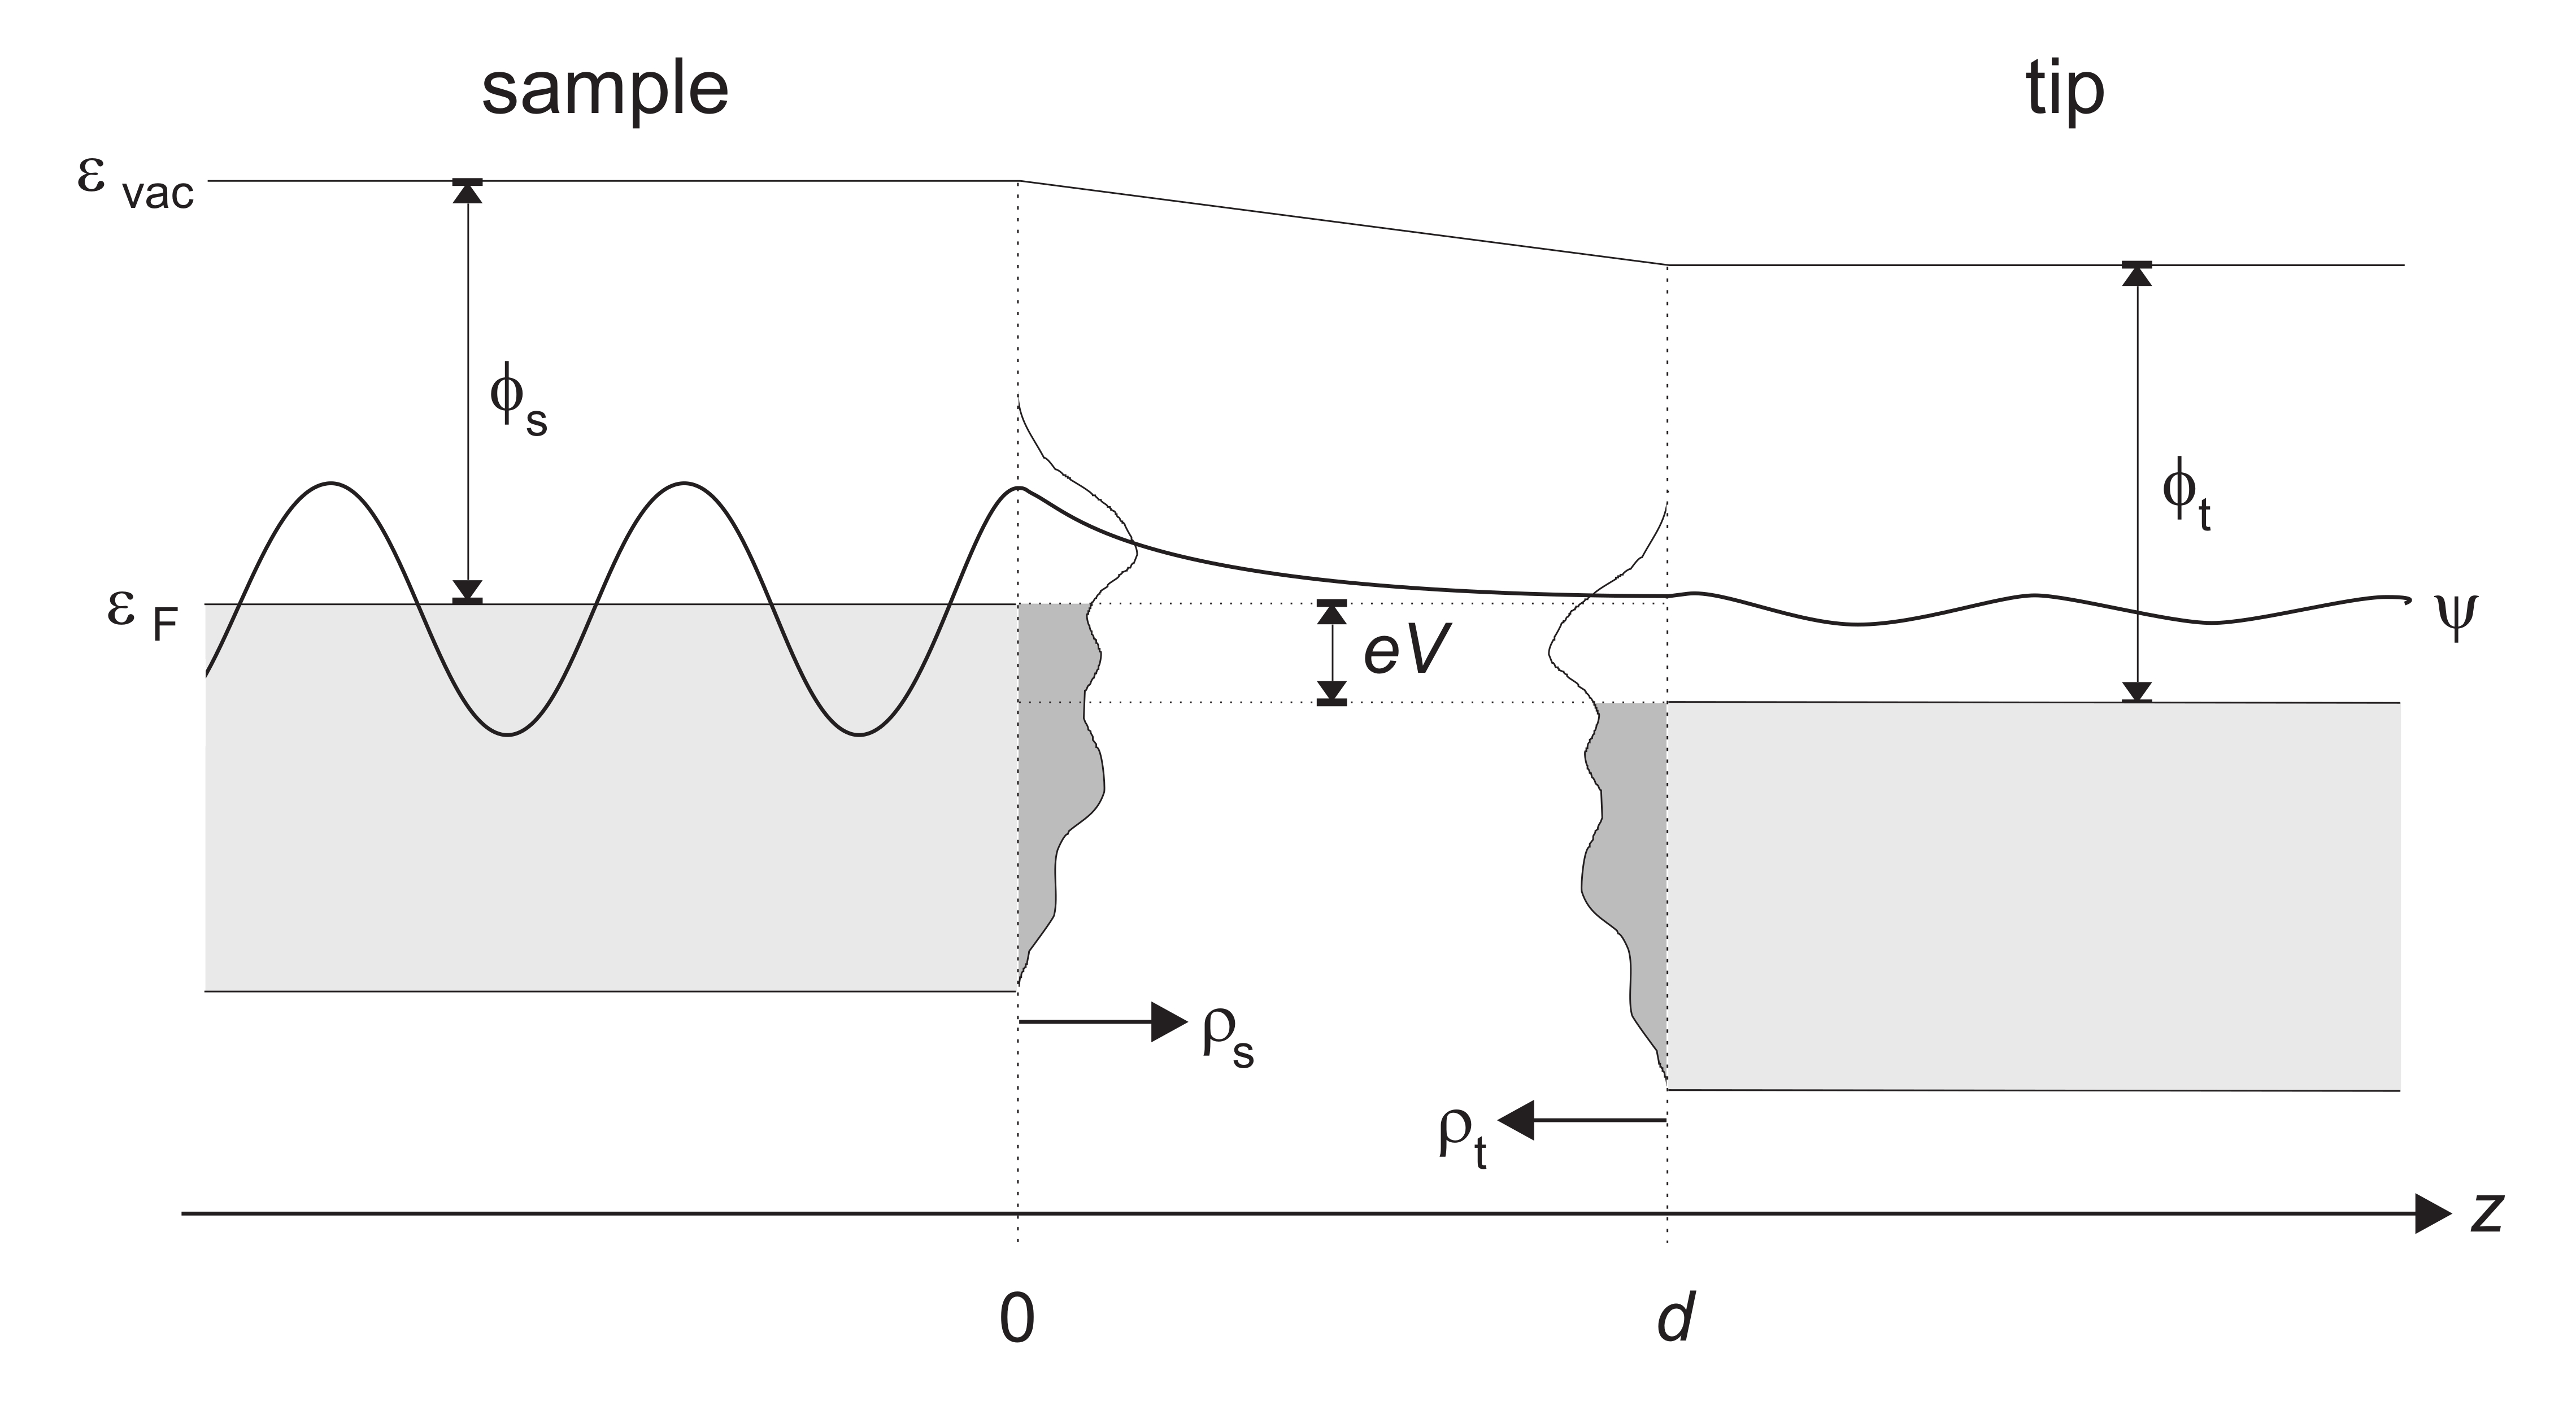
\includegraphics[width=0.7\textwidth]{./images/tunnel-barrier}
	\caption{Energy diagram to visualize the tunneling process between sample (left) and tip (right) separated by a distance d. Work functions of sample and tip ($\Phi_s$ and $\Phi_t$) separate the filled states (shaded regions) and the vacuum level ($\epsilon_{vac}$). Since sample ($\rho_s$) and tip DOS ($\rho_t$) may not be uniform, a fictional DOS is sketched in darker colors between both. The samples energy is lifted by $eV$ after a bias is applied and results in a net electron current from the sample into the tip. One tunneling process is indicated by a wave function $\Psi$ in the sample. After overcoming the vacuum barrier its amplitude decreased and the corresponding electron occupies a free state (white) in the tip material.  Adopted from \cite{diss-schunack}}
	\label{fig:STM-barrier}
\end{figure}

Consider a system where two metals (sample and tip) are separated by a vacuum gap. 

The amount of energy needed to remove an electron from the metals highest occupied energy level ($E_F$, Fermi energy) is called work function $\Phi$. It depends on the electrostatic potential $\phi_E$ that has to be overcome by an electron charge $e$ at the surface.
$$ \Phi = -e \phi_E - E_F $$

\autoref{fig:STM-barrier} shows an energy diagram for tip and sample. The work function $\Phi_s$ (sample) and $\Phi_t$ (tip) separates the vacuum level $\epsilon_{vac}$ and Fermi energy $E_F$.

If sample and tip are in thermodynamic equilibrium, their Fermi energies are equal.
When both are brought in close contact, electrons from the sample tunnel into unoccupied states of the tip and vice versa in the same number. Hereby electrons close to $E_F$ have the largest decay length and attenuate less strong in vacuum and contribute strongest to the tunneling current. This current can be modeled and calculated in simple systems. 

%\paragraph{STM}
In the model of Tersoff-Hamann\index{STM!Tersoff-Hamann}\footnote{Please's note that there are more models and corrections to them. An evolution from Bardeen's approach to the one done by Tersoff-Hamann can be found here \cite{lounis_theory_2014, wortmann_interpretation_2000} including Chen's expansion.} the tip is atomically sharp and its electrons waveform is s-like. Further assuming low temperature and a constant band structure for the tip with apex radius R, it is possible to calculate the tunneling current $I$. 

$$I \propto U \cdot \rho_t(E_F) \cdot \rho_s(E_F) \cdot \kappa^{-4}R^2e^{2\kappa R} $$

With this theory constant current STM images image the surface density of states for  a given voltage $U$. The exponential decay ($\propto e^{-\kappa d}$) of an electron wave function into vacuum is characterized by $\kappa=\frac{\sqrt{2m\Phi}}{\hbar}$. It limits the current, which is proportional to the squared amplitude of it. 

$$I\propto e^{-2\kappa d}$$

Like in one dimension the current depends on the barrier height $\Phi$ through $\kappa$. Increasing the distance exponentially decreases the tunneling current.\footnote{http://pmrb.free.fr/work/diplom/html/mainse2.html} This exponential relation is the reason for the excellent topography resolution capabilities of STM.

While its a good first approximation of the system, in many cases more than just the electrons near Fermi contribute. Also a uniform $\rho_t(E)$ may not be accurate in all cases.

Using \index{STM!WKB} Wentzel-Kramers-Brillouin (WKB) theory\cite{wentzel_verallgemeinerung_1926, kramers_wellenmechanik_1926, brillouin_mecanique_1926} the tunneling current is given by
\begin{equation}
I=\int_0^{eV}\rho_s(r,E)\rho_t(r,eV+E)T(E,eV,r)dE
\label{WKB}
\end{equation}
where $\rho_s(\rho_t)$ is the density of states of the sample (tip) and T is the tunneling transmission probability
\begin{equation}
T(E,eV)=exp\left(-\frac{\textcolor{red}{\textbf{2}}Z\sqrt{2m}}{\hbar}\sqrt{\frac{\Phi_s+\Phi_t}{2}+\frac{eV}{2}-E}\right)
\label{Transmission-function} 
\end{equation}
describing the probability of an tunneling event between tip and sample.

The samples potential can be changed by applying a voltage $V=U_b$ (bias) to it. This lifts its Fermi energy with respect to the tips and leads to a net electron current from the sample into the tip. Reversing the voltage results in electrons tunneling from the tip into the sample. If $eV<0$ the tunneling current is largest for $E=0$ (electrons on the Fermi-level of the sample), if $eV>0$ the tunneling current is largest for $E=eV$ (electrons of Fermi level in tip).

Due to the fact that the tunneling current is proportional the density of states in the tip and the molecule one can deduce the band structure within a range of several volts in the vicinity of the Fermi energy. Investigation of this behavior led to the establishment of a new measurement technique, called scanning tunneling spectroscopy (STS).

\subsection{\textbf{S}canning \textbf{T}unneling \textbf{S}pectroscopy}
\label{section:STS}
Changes of the tunneling current with the bias voltage were observed by Tromp et al. in 1986 \cite{tromp_atomic_1986}. They discovered a change in contrast when scanning a SI(111) surface with either positive or negative bias. The change in contrast is most apparent in semiconductors and semi metals\cite{bonnell_scanning_1993}, but adsorbates and charged areas of the sample change the DOS locally and therefore the contrast in STM. While simple results may be already obtained by comparing two images recorded at different biases, more detailed information can be achieved.

\index{STS!Bias below work function}
If tunneling conditions are such that $eV\leq\Phi$, observed features in $dI/dV$ are associated with the surface DOS. Critical points in the surface projected DOS give rise to features in dI/dV. Interpretation of these features with the WKB theory (i.e. differentiating equation \eqref{WKB}) gives
$$dI/dV=\rho_s(r,eV)\rho_t(r,0)T(\textcolor{red}{\textbf{eV}},eV,r)+\int_0^{eV}\rho_s(eV)\rho_t(r,E-eV)\frac{dT(E,eV,r)}{dV}dE$$
The first term contains the DOS of the sample and tip and the transmission function. While it is usually unknown, a closer look to \eqref{Transmission-function} indicates a smooth, monotonically increasing function in V. This mannered dependence on V gives a smooth background described by the second term $\int_0^{eV}\rho_s(eV)\rho_t(r,E-eV)\frac{dT(E,eV,r)}{dV}dE$.
The first term $\rho_s(r,eV)\rho_t(r,0)T(\textcolor{red}{\textbf{eV}},eV,r)$ describes the dependence on the DOS in the sample for energies $eV$ - our desired spectrum. As for STM topography images, bias voltage can be chosen to either probe occupied ($U_b < \SI{0}{\volt}$) or unoccupied states ($U_b > \SI{0}{\volt}$).  At low temperatures the vanishing lateral movement of adsorbates makes them also accessible to tunneling spectroscopy with sub molecular lateral resolution. It is possible to deduce the electronic configuration with atomic spatial resolution.

\subsection{Machine description and experimental details}
The success of STM and STS is promoted by good mechanical engineering. Since distances down to the atomic length scales are investigated, the experiment needs a careful set up. This is true especially for damping of external vibration that would otherwise conflict with the measurement. Sufficiently low partial pressures are needed to achieve little contaminant adsorption and the long investigation times associated with it.

Since all used UHV chambers have many common parts, a typical setup is described with the low temperature (LT) STM setup. Here the most experiments were carried out.

The central part of the LT-STM setup is the commercial \textbf{Beetle-type STM scanner} \cite{zoephel_aufbau_2000} as shown in \autoref{fig:stm-heliocoidal-ramp}. Here a helicoidal ramp carries the central scan piezo with attached STM tip. Three outer piezo tubes are used in slip-stick motion to circularly move on the ramp. Because the ramp is cut with an inclination of \SI{2}{\degree} the circular motion of the piezos results in the STM tip moving up and down. This is used to control the height above the sample during tip approach and macroscopic lateral movement.

A separate piezo is used to control the lateral position of the tip during scanning. With it the image width, scan speed and tip-sample distance can be controlled on a continuous, sub-atomic length scale (\autoref{fig:STM-tip}).

Not only the macroscopic movement of the STM stage is controlled with a set of piezos, but the position of the tip (x, y, z) during scanning, too (see \autoref{fig:STM-tip}). In this work a segmented tubular piezo is used to control the tips position. The piezos elongation can be controlled with the voltage applied to them, which is used to choose not only the tip-sample distance. Lateral movement is done by addressing its four segments. Each is used to control movement along $\pm \textnormal{x}$ and $\pm \textnormal{y}$ direction and controlled by the feedback loop. For recording an image the area is raster scanned in consecutive lines, applying a sawtooth voltage to the fast scan direction. The next lines are chosen by stepwise increasing the voltage along the slow scan direction. Other parameters like image size and scan speed are controlled wit the piezos as well.

The measured current is translated into a voltage (I/U converter) and processed in a 20 Bit digital $\rightarrow$ analog (D/A) converter. The current intensity is feed into the Digital signal processor (\textbf{DSP}) board. Here the STM Software's current set point is compared with the measured value. The tips position is controlled with a feedback loop. If the tips position needs to be corrected, a voltage is passed through a HV amplifier and is applied to the corresponding piezo element. 
%The DSP is used to attenuate high frequency components. \textcolor{red}{\textbf{ More detail?}}

Differentiation of the current signal is done with an \textbf{Lock-In Amplifier}. Here the spectrum is not recorded directly by sweeping the bias and numerically differentiating the measured current. A sinusoidal modulation on top of the bias voltage with a frequency higher than the low pass frequency of the DSP is used. The modulated bias leads to a tunneling current modulation with the same frequency. The differentiation is performed by reading the AC current signal with the same frequency as the modulation which directly gives the dI/dV signal and therefore the DOS of the sample at $U_b$. 

Because the Lock-In Amplifier then only takes signals with the same frequency than the excitation frequency into account, the results are much less suspect to noise. Compared to numerical differentiation, a Lock-In needs less computing effort, too. It is important to note that the DSP does not recognize the bias/current modulation as topographic feature and regulates as without modulation. If the modulation frequency is too low, the feedback tries to compensate the modulation by changing the distance to the sample. If the modulation frequency is too high, the capacitance between tip and sample leads to an $90\deg$ phase shifted current which increases with modulation frequency. One usually chooses the modulation frequency slightly above the cutoff frequency for the feedback loop.

\begin{wrapfigure}{O}{5cm} \centering
	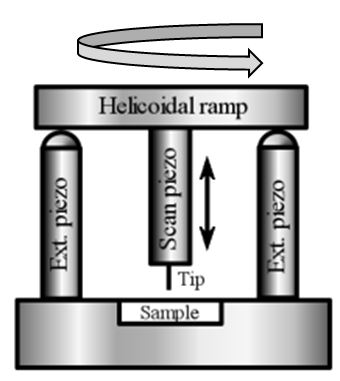
\includegraphics[width=4cm]{./images/STM-sketch-2}
	\caption{STM sample stage to control the tip position. The coarse movement is controlled by exterior piezos. Each moves on a heliocoidal ramp with slip-stick motion. The precise positioning during scan is done with a central piezo to which the tip is attached. Modified from \cite{heliocoidal_ramp_2018}.}
	\label{fig:stm-heliocoidal-ramp}
\end{wrapfigure}

To maintain UHV conditions, a set of pumps is used. For the preparation chamber, where high partial pressures occur during sample cleaning and preparation, a combination of roughening and turbo molecular pumps is used. First a roughening pump lowers the atmospheric pressure to \SI{1}{\milli \bar}. With this pressure on the outlet side a turbo molecular pump is used to decrease the pressure even further to the  \SI{1e-8}{\milli \bar} range. The remaining pressure is caused by adsorbate covered chamber walls where continuous ad-/desorption takes places and maintains a pressure equilibrium. After heating the entire chamber to temperatures above \SI{120}{\celsius} while constantly pumping, most of the water is desorped from the walls and pumped. After cooling down to room temperatures, the pressure settles in the \SI{5e-10}{\milli \bar} regime.

As the pumping efficiency of turbo molecular pumps decreases for low pressures, each chamber is equipped with an ion getter pump. Here a high voltage \SIrange{1}{7}{\kilo \volt} is applied between two getter materials. Residual gas particles ionize in the strong electric field and are accelerated towards the plates. Here they impinge with high velocity and are buried deep in the plate material that they can't leave. The reduced number of residual gas particles results in a lower pressure.

To further reduce the number of potential contaminations, parts of the chamber can be cooled down with liquid nitrogen. Because of the great temperature gradient, gaseous residuals condense on the much colder surface of the cooling trap and remain adsorbed while the temperature is kept low. Without refilling with liquid nitrogen the temperature slowly increases over time, so that the cooling trap looses pumping efficiency over time (usually after \SIrange{1}{2}{\hour}) and starts to release trapped contaminants again.

A titanium sublimation pump is installed to evaporate titanium on demand. This covers the chamber walls and, due to its reactivity, binds residual gas. After some time the reactivity diminishes and a new layer has to be evaporated. With routine operation intervals the base pressure of the UHV system can be improved permanently.

While LT-STMs may be operated with solely helium, it is more resource saving to only cool the direct proximity of the sample and the STM with He and to suppress the heat flow out of the He cryostat with a second surrounding nitrogen cryostat (boiling point: \SI{77}{\K}, compare figure \ref{fig:STM-cryo}). This diminishes consumption of globally limited He. To maintain a temperature of \SIrange{5}{7}{\K}, one to two liters of liquid helium are evaporated a day, plus an additional amount of three to four liters liquid nitrogen. Evaporated helium is reclaimed in a closed circuit with a system of purifying and storage/cooling steps so that only a small amount of helium escapes the circuit and is lost.

Sample temperatures down to \SIrange{5}{7}{\K} allow for observations not possible at elevated temperature. Cooling not only reduces thermal drift in the piezo elements that are used to control the tip's position on the sample. Thermal energy at low temperature is not high enough for atoms or molecules to move on most substrates. Species mobile at room temperature (and therefor not representable at room temperature in the sub-ML regime) become immobile and accessible for ST microscopy and spectroscopy. ST spectra resolution is better at low temperatures.

\begin{figure}[ht]\centering
	\subfigure[LT-STM setup. Different functional groups are highlighted by colors. A low base pressure in achieved with a combined pumping system comprised of ion pumps and turbo molecular pumps (cyan). The liquid helium/nitrogen bath cryostat (red) is used to maintain low temperatures. Sample holders are operated with a rote able, variable temperature manipulator (green). Sample preparation is done in the preparation chamber (blue). After transfer to the LT-STM chamber (yellow) a gate valve is used to seal the LT-STM from remaining residual gas that may be present in the preparation chamber. Vibration isolation of the frame is achieved with legs floating on pressurized cylinders (orange).]{
		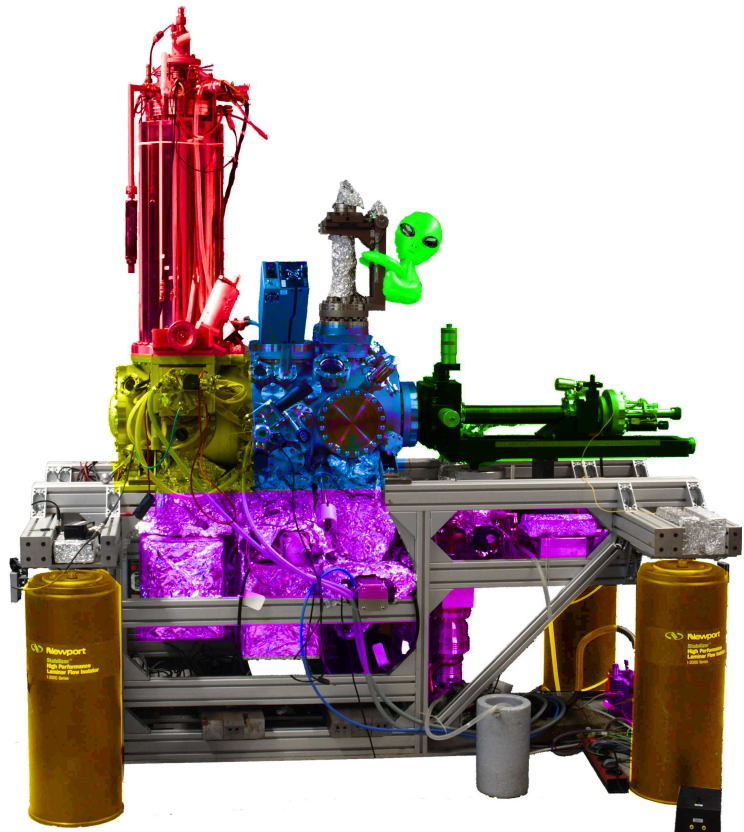
\includegraphics[width=0.45\textwidth]{./images/chamber-sketch.jpg}
		\label{fig:chamber-sketch}
	} \quad
	\subfigure[Scheme of a liquid bath cryostat. While in the inner stage a temperature of \SIrange{5}{7}{\K} is achieved with a liquid helium reservoir, an outer liquid nitrogen cryostat is used to isolate the inner cryostat from the surrounding room temperature and to reduce the amount of liquid helium used to maintain cryogenic temperatures.]{
		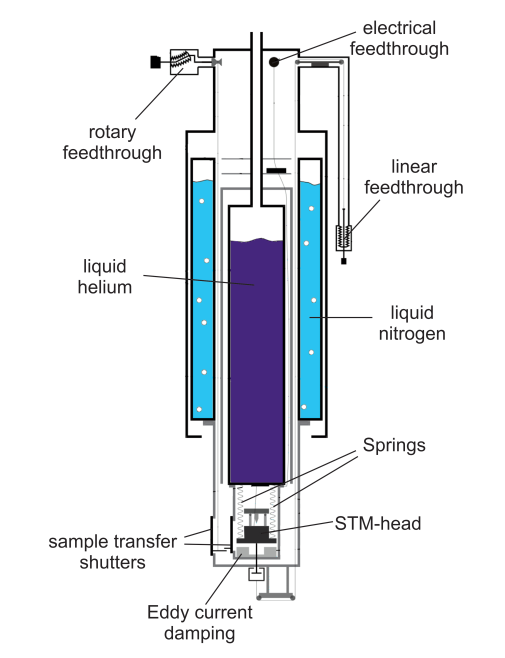
\includegraphics[width=0.45\textwidth]{./images/sketch-cryo.jpg}
		\label{fig:STM-cryo}
	}
	\caption{Typical setup for low temperature measurements. A vibration isolated UHV chamber is used to prepare samples and investigate them in a separable chamber with either STM or AFM. A liquid bath cryostat is used to maintain low temperatures. Images adopted from \cite{diss-knud}}
	\label{fig:STM}
\end{figure}

\begin{figure}\centering
	
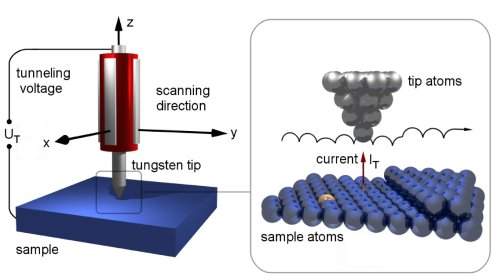
\includegraphics[width=0.6\textwidth]{./images/stm-rutgers-modified.jpg}
	\caption{Operating principles of an STM. A macroscopic sketch  shows the central piezo that controls the tip position on the sample. The piezo is divided in four parts to control movement in the x-y plane and tip-sample distance. A microscopic sketch shows the tips movement in constant current mode while moving across a atomic step edge. Here the tip is retracted to maintain a constant current, which in turn leads to a larger apparent height in STM. Note the single incorporated alien atom. Although its height is the same as its neighbors, STM records the change in DOS. Less electrons tunnel and the apparent height on the terrace is reduced above the alien atom. Adopted from \cite{STM-rutgers}}
\label{fig:STM-tip}
\end{figure}

Two damping stages are used, one for the chamber and a sequential one for the STM.

First the whole UHV system is placed on air pressurized cylinders. These can be lifted on demand, so that the chamber floats on four dampers and external vibrations/shocks are damped. 

A second stage decouples the sensitive STM scanner from the rest of the setup. First the complete STM stage hangs on springs to further limit the direct influence of vibrations. Second the remaining oscillation amplitude is damped by a eddy current damping. It is made of three magnets in close proximity to the surrounding conductor so that eddy currents are induced for each movement. The eddy current is typically larger at cryogenic temperatures, that results in a damping that works best at low temperatures. The kinetic energy of the oscillating system is transferred by the eddy currents into heat within the surrounding support. The heat is then mitigated by the external cooling of the cryostat.

\paragraph{Experimental details}

\textbf{Topography images} are created by raster scanning the surface pixel by pixel. 
We use the constant current (cc-STM) operating mode where the tips height is controlled to achieve a constant tunneling current as shown in \autoref{fig:STM-tip}. The regulating voltage on the height control piezo is recorded and plotted in an color-scale for each pixel. The brighter the color, the more the piezo had to retract the tip to maintain a constant tunneling current. Regions with the same DOS thus appear in the same contrast.

%	A modified tip allows for real space imaging of molecular orbitals.

\textbf{dI/dV} is performed in two ways - on single points (spectrum) and on areas (map). 

\textbf{Single point spectra} are used to measure electronic properties like molecular orbital energies and electronic band gaps.
Spectroscopic information can be obtained by either changing the bias voltage and tip height (I(V,z)-spectroscopy) or the tip-sample distance (V(z)-spectroscopy) (I=const).   

\textbf{Spectral maps} at a fixed bias show real space distribution of electronic states at the DOS that corresponds to the chosen bias. The signal intensity represents the differential conductance $\propto$ DOS. Differentiation is done with a Lock-In (see paragraph above). For dI/dV maps the feedback loop that controls the tip vertical position is not in use, so that the tip maintains an even height.

\textbf{Lateral manipulation} of atoms and molecules is possible with the STM tip. With a matching current/voltage setpoint, the tips vertical position can be chosen such that the tip interacts with the adsorbate. Lateral displacement of single molecules within molecular assemblies is only possible if molecule-molecule interactions are weak, e.g. no covalent bonds are formed between molecules. 

\subsection{Limitations}\index{STM:resolution}

The accuracy of a STM is very high with spatial resolution down to the atomic scale.

\textbf{Lateral resolution} with the STM depends on the tip shape and termination. A tip with single atom termination records sharp topography images. When there is more than one atom in the tip apex participating in the tunneling process lateral resolution decreases and each creates its own image with partial overlap.

\textbf{Spectral resolution} is influenced most by the tip DOS. Before each measurement a reference spectrum is recorded on the metal surface to ensure the the DOS fo the tip in metallic and does not show unexpected additional states that are typically induced by a modified tip.

Due to the fact that the tips motion is controlled with different piezos, one has to take different elongations in different directions into account. For example, if the STM scans the fast scanning direction just a bit further than the slow scan direction, the resulting image (although pixel wise square) is no longer physically square anymore. 
%Imagine a square (1:1 side ratio, diagonal angle 45\textdegree) where one side is elongated by 5\%. The resulting square (1:1.05 side ratio, diagonal angle 43.6\textdegree) looks square because it has the equal number of pixels in both directions, but it is physically rectangular. The expression used to calculate the uncertainty with known calibration parameters is
%$$\Delta \Theta = 45 - \frac{180}{\pi}\cdot\arctan(\frac{1}{1+x})$$ where x is the percentage of one side being longer. This results in an uncertainty of 0.3\textdegree(1\%), 1.4\textdegree(5\%, see example above), 2.7\textdegree(10\%). 
For moderate shear below \SI{5}{\percent} however, conformity is almost conserved and the angular uncertainty below \SI{1.5}{\degree}.

Because STM is sensible to electronic changes, it may change the footprint of an adsorbed compound \cite{sautet_interpretation_1992}. When laterally approaching an adsorbate this results in an additional tunneling current, because now electrons do not only tunnel directly into the substrate but through the adsorbate as well. Interferences between both tunneling processes depend on the adsorbate's orbital-symmetry and tip-shape. Local density of states calculations \cite{tersoff_theory_1985, lang_theory_1986, eigler_imaging_1991} are not adapted to grasp this effect since the tip is considered far away from the surface. Moreover, the tip radius or the tip-substrate distance is often optimized to fit the lateral size of the adsorbate print with the experimental image \cite{tersoff_theory_1985, eigler_imaging_1991}. 

The tip termination was changed in different ways. 
1. \textbf{Tip forming:} 
		A voltage pulse ($U_b \leq \SI{10}{\volt}$) is given for a short time ($t \leq \SI{1}{\second}$) when the tip is in tunneling contact. The intense current pulse reorders the tip termination.
2. \textbf{Vertical over-approach:}
		The tip is pushed into the sample surface in order to remove tip adsobates.
3. \textbf{Field emission:}
		An external power supply is used to apply a voltage ($U_b$=
		\SIrange{100}{500}{\volt}) between tip and sample. A serial resistor limits the current through the connected internal wires. Tip and sample are brought in close proximity to enable the tunneling process. Because of high electrical field strengths at the tip apex strong forces occur. Depending on the polarity the tip can either aggregate sample surface atoms or expel tip atoms. Careful distance increase then builds up a new tip apex.
The above mentioned ways are done with the tip remaining inside the STM.
4. \textbf{Tip sputtering:}
		To reorder the tip structure and to remove adsorbates accelerated Ar$^+$ ions are used. Because of higher partial pressures needed for sputtering the sample is transferred from the LT-SMT into the preparation chamber.

Mechanical and thermal vibrations limit the resolution of STM and STS, too. Therefor the damping stages that decouple the STM from the surrounding are important but may not always filter all mechanical vibrations. 

Signal wires are well shielded against electromagnetic radiation. Since the signal is transmitted with cables an external radio signal may otherwise couple into the wire and tamper with the signal.

Although STM works at room temperature, additional cooling may be applied to reduce the thermal vibrations.

STM is not capable to discern different elements. As complimentary method, X-Ray photoelectron spectroscopy is used for chemical identification of adsorbates.
  \section{\textbf{X}-ray \textbf{P}hotoelectron \textbf{S}pectroscopy}
  \label{section:xps}
	\label{section:XPS}\index{XPS} 
\textbf{X}-Ray \textbf{p}hotoelectron \textbf{s}pectroscopy (XPS) is a tool to achieve information of the samples chemical structure.
When X-rays with sufficient energy hit metals, electrons are emitted. This effect is called photoelectric effect and was first discovered by Heinrich Hertz in 1887 through the fact that electrodes illuminated with ultraviolet light create electric sparks more easily. \cite{hertz_ueber_1887} 18 years later Albert Einstein received the Nobel Price for his discovery of the law of the photoelectric effect\cite{_nobel_2015} and a scientific explanation which Hertz was missing. The emitted electron's kinetic energy depends on the element the electron was emitted from and allows for exact identification of the atomic species on the sample.

\subsection{Theory}
\index{XPS!Physical model}As the X-rays hit and penetrate the sample surface they excite electrons and initiate core-level excitations.

For the \textbf{core-level excitation} the X-ray removes a single electron strongly bound to the core. Energy conservation due to elastic scattering of the electron out of the bulk results in the relation 
\begin{align}
%E_{kin} &= h\nu_{\textnormal{X-ray}}-E_{B}-\Phi_{\textnormal{analyzer}} \\
E_B 	&=h\nu_{\textnormal{X-ray}}-E_{kin}-\Phi_{\textnormal{analyzer}}
\end{align}
 $h\nu_{\textnormal{X-ray}}$ is the energy of the incident X-ray beam, $E_B$ the binding energy of the excited electron and $\Phi_{analyzer}$ the work function of the analyzer. The stronger the binding energy, the less energy is left for kinetic energy.


\begin{figure}\centering
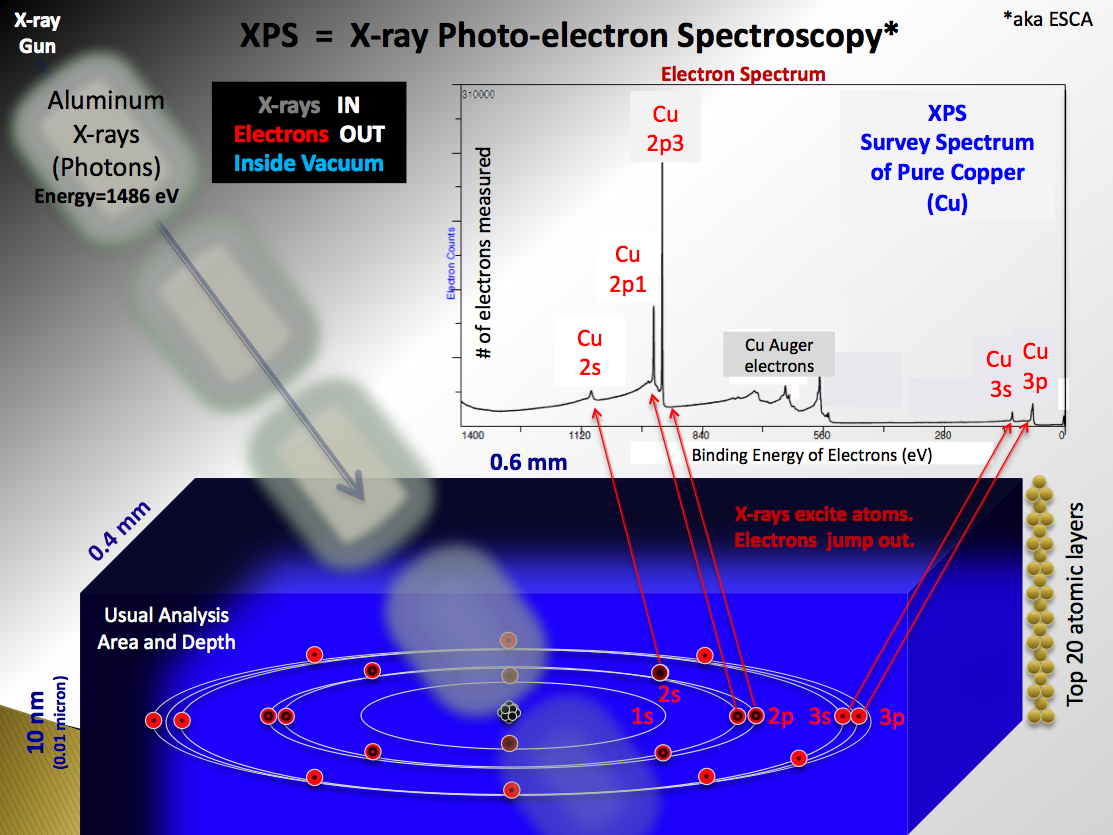
\includegraphics[width=0.7\textwidth]{./images/XPS_PHYSICS}
		\label{fig:XPS-excitation}
	\caption{Representation of a XPS process. A scheme of a X-ray gun illuminating a sample area of about \SI{0.4}{\milli \meter} $\times$ \SI{0.6}{\milli \meter} is shown. X-rays are used to excite core level electrons. Excited electrons within the first 20 layer escape the sample. After leaving the sample these show element specific signatures in their kinetic energies. A detailed analysis of the peak shift allows for identification of the chemical environment.}
	\label{fig:auger-core}
\end{figure}

\cite{zemlyanov_versatile_2018}
The \index{XPS!chemical surrounding} \textbf{chemical surrounding} of atoms changes their binding energy, making XPS an ideal tool to detect changes in chemical surrounding. Although the analysis is averaged over the area of the incident X-rays its results are very precise. This makes it possible to distinguish differently bound atoms within single atomic species and therefore gives rise to otherwise not directly observable processes like growth, intercalation, etching and binding of for example 
graphene islands on Ir(111)\cite{busse_graphene_2011-1,granas_oxygen_2012}.
The \index{XPS!binding energies} binding energies of some atomic transitions are given in \autoref{tab:XPS-intensities}.

\begin{table}\centering
 \caption{Element specific transitions and binding energies for some chosen elements as reported in \cite{wanger_handbook_1979}}
 \begin{tabular}{lll}
  Element & Ground state & $E_B$ [eV]\\ \hline 
  O & 1s & 531\\
  N & 1s & 398.1\\
  C & 1s & 285\\
  B & 1s & 189.4 \\
%  Cu & 2p $\frac{1}{2} (\frac{3}{2})$ & 953 (933) \\
%  Cu & LMM & 560-580 \\
  Cu & 3s & 123\\
  Cu & 3p $\frac{1}{2} (\frac{3}{2})$ & 77 (75)\\
 \end{tabular}
\label{tab:XPS-intensities}
\end{table}

The shape of the peaks typically resembles the line shape of the used X-rays (Gauss width $\approx 1eV$). In case of s-states $(l=0)$ (B\textit{1s}, N\textit{1s}, C\textit{1s}) the peaks are singlets. With increasing $j=l+s$, the spin-orbit (j-j) coupling introduces a 'parallel' and 'anti-parallel' nature of the spin, resulting in two different $j=\frac{1}{2}(\frac{3}{2})$ and therefore two different energies.
% The split in energy is expected to increase with the atomic number Z (for constant n,l) or as l decreases (n constant). This makes the splitting of 3p orbitals larger than that of the 3d's. 
The ratio of the two peaks is given by their degeneracy $(2j+1)$\cite[113]{Riviere_90}, so that the $\textnormal{Cu3p}\frac{3}{2}$ peak is two times larger than $\textnormal{Cu3p}\frac{1}{2}$.

\subsection{Experimental details}
The \textbf{X-ray sources} used are supplied with aluminum and magnesium anodes.
%\footnote{Other materials are available that produce various X-ray energies and line widths \index{XPS!Anode materials} \cite{_x-ray_2015}.} 
With these, electrons are accelerated with typically \SI{15}{\keV} onto the anode of choice. Most of the created radiation is made up of the principal characteristic line ($K\alpha_{1,2}$). Higher ones ($K\alpha_{3,4}$, $K\beta$) are also observed but with much lower intensities. In addition there is a continuous background called Bremsstrahlung extending up to the energy of the incident electron energy. This background is of no use for the XPS measurement and has to be subtracted in a more or less artificial way. For XPS measurements the Mg K$\alpha$ = \SI{1253.6}{\eV} and Al K$\alpha$ = \SI{1486.6}{\eV} are used situationally to shift the core level spectra with respect to substrate transitions (Auger transitions) at constant kinetic energy.

The more atoms of a specific kind are present, the larger the signal gets. Therefore the signal intensity resembles the amount of atoms on the topmost surface layers($\approx \SI{10}{\nm}$). As each irradiated atomic species has a different \textbf{cross section} for adsorption of X-rays with a certain energy they emit spectra with a different intensity. Comparing the cross section of e.g. N and B, one can see that it it roughly 4 times as large (B: \SI{6,87e3}{\barn\per atom}, N: \SI{25,82e3}{\barn\per atom}) for $\textnormal{Al} K_{\alpha}$\cite{henke_x-ray_1993}. Meaning that the signal from the N is much stronger than that of the B, although their number of atoms is equal.

\textbf{Gracing and normal emission} are two operational modes in XPS. The maximum information depth in XPS measurements is mainly limited by the escape length of excited core level electrons ($\approx \SI{10}{\nano \meter}$) for electrons. The mean free path of electrons with energy E in a solid is approximated by $\lambda = \frac{143}{E^2} + 0.054 \sqrt{E} \stackrel{E=\SI{1}{\kilo \eV}}{\approx} \SI{1.7}{\nano \meter}$.\cite{Seah_Quantitative_1979} This is much smaller than the penetration depth of X-Rays which are in the order of \SI{10}{\nano \meter}. An increasing angle between sample and detector increases the path the electrons have to travel through the bulk to reach the analyzer. Because the mean free path of the electrons stays the same, a longer route in the bulk attenuates the signal of lower lying substrate atoms. Electrons leaving the surface adsorbate are not attenuated and gain in signal strength relative to the bulk atoms.

Some supporting measurements are done in gracing emission to increase an otherwise small signal of an surface adsorbate but are not shown in this work.

The spectra used in this work are recorded without monochromator. Experiments are done at two different XPS setups. (1) The RT-STM/XPS (2) The NIM-XPS chamber.  

\subsection{Limitations}
\paragraph{Beam damage}
Since the X-Rays carry considerable energy other effects than the excitation of core electrons are possible. Especially for long integration times of the analyzer (for elements with little cross section or little surface coverage) the amount of deposited energy results in unwanted side reactions on the surface. It is possible to trigger a change in the chemical surrounding of the investigated element, causing chemical shifts that are not present in the pristine sample and change the XPS spectrum over time.

\paragraph{Space averaging technique}
XPS is a space averaging technique. First the X-Ray beam has an inherent width, the analysis area can't be chosen arbitrarily small. Second, X-Rays do excite electrons not only directly within the illuminated area, but penetrate the bulk and cause a cascade of transitions in the sample. The resulting information is always a mix between surface adsorbates and bulk elements.
  \section{\textbf{A}tomic \textbf{F}orce \textbf{M}icroscopy}
  \label{section:afm}
	\textbf{A}tomic \textbf{f}orce \textbf{m}icroscopy (AFM) is like STM another scanning probe tool. To scan the surface of the sample, one uses an small oscillating tip to interact with it on short distance where forces between sample and tip occur. If the tip interacts with the sample, its oscillation is hindered/amplified and the frequency of the oscillation shifts. 
From this shift one can estimate the strength of the acting force. Since every type of adsorbate atom acts in different ways with the tip, AFM is element specific. When the tunneling current through the AFM tip is recorded, simultaneous AFM and STM measurements are possible. 
\subsection{Theory}

\begin{figure}\centering
	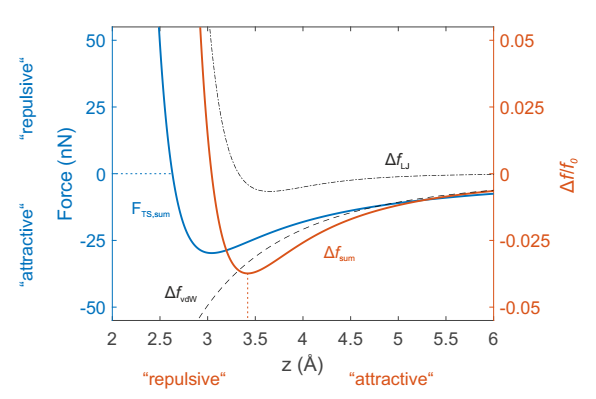
\includegraphics[width=0.7\textwidth]{./images/AFM-graph-martin}
		\label{fig:AFM-force}
\caption{Sketch of tip-sample interaction force (blue) together with relative frequency shift. Contributions of vdW and Lennard Jones like forces result in two separable frequency shifts $\Delta f_{LJ}$ and $\Delta f_{vdW}$ (black) that add up to a total of $\Delta f_{sum}$ (orange) from where the total force is derived. From \cite{schwarz_assembly_2018}}
\label{fig:AFM-sketch}%
\end{figure}

Amongst others, forces between AFM tip and sample are made up of attractive forces like van der Waals (vdW) forces and repulsive forces like mechanical contact force and Pauli repulsion.

vdW interaction is always attractive and described by
\begin{equation} \label{eq:vdW}
F_{vdW} = - \frac{A_H R}{6z^2}
\end{equation}
Here $A_H$ is the \textcolor{red}{\textbf{?}}, $R$ \textcolor{red}{\textbf{?}} and $z$ \textcolor{red}{\textbf{?}}. Although the strength quickly diminishes with distance $z$, vdW interaction is long range and thus always present in AFM measurements.

Mechanical contact force, Pauli repulsion and chemical bonding are given in the Lennard Jones (LJ) model.\cite{jones_determination_1924}
\begin{equation} \label{eq:LJ}
 F_{LJ} = - \frac{12 E_{min}}{z_0} \left ( \left (\frac{z_0}{z} \right ) ^{13} - \left ( \frac{z_0}{z} \right )^7 \right )
\end{equation}
$E_{min}$ is \textcolor{red}{\textbf{?}}.

The typical resulting force between tip and sample $F_{TS,sum}$ is artistically shown in \autoref{fig:AFM-sketch}. 
%On the top part a tuning fork with an atomic tip is shown on top of the sample surface. The interaction forces $F_{ts}$ act between tip and sample and are indicated by an arrow. In the lower part a representation of the resulting force in dependence of the tip-sample distance is shown. 
The sum of interaction $F_{TS,sum}$ between tip and sample is shown as blue  line. The attractive vdW force is plotted in dashed black curve. A typical frequency shift $\Delta f_{sum}$ is given as orange graph. The frequency shift $\Delta f$ is proportional to the force gradient acting on the tip.

$$\Delta f = - \frac{f_0}{2k_0}\frac{\delta F_{TS}}{\delta z}$$

One can distinguish different regimes as indicated by the labels. When tip and sample are in considerable distance to each other, the attractive vdW forces are the dominant part in the sum. While the tip approaches the sample, more and more interactions with the surface and adsorbate add to this force, increasing $F_{TS}$. When the separation reaches $z_0$, the distance becomes so small that repulsive forces overcome the attractive one at the boarder to the repulsive regime.

%AFM is used here in the non-contact mode (\textbf{nc-mode}): The tuning fork is driven at its resonance frequency with fixed amplitude and at a certain distance to the sample. Long-range forces like van-der-waals and others change the resonance frequency of the cantilever. This change is a indication of the acting force between cantilever and sample. 

AFM measures does not measure a mix of electronic and geometric information projected onto a 2D-map like in STM.

To increase the lateral resolution the tip can be functionalized with CO. This method is widely used \cite{albrecht_direct_2016, kawai_multiple_2018, kawai_atomically_2015, schulz_elemental_2018, gross_chemical_2009, pavlicek_generation_2017, schwarz_corrugation_2017} to investigate not only geometric features that are not directly accessible in STM, but also chemical differences on the sample.\cite{wang_exploration_2017}

\begin{figure}\centering
	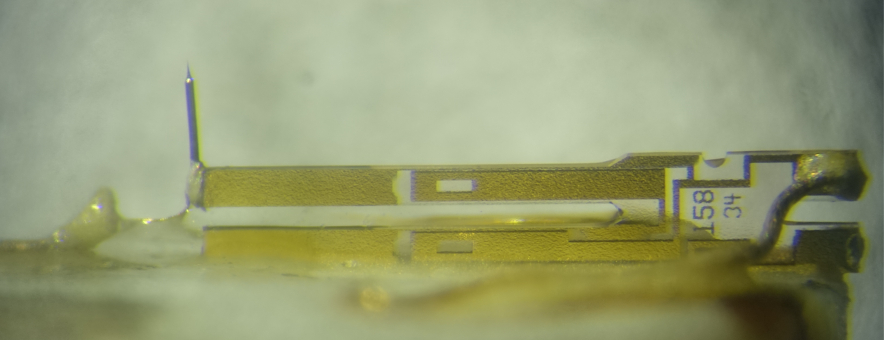
\includegraphics[width=0.7\textwidth]{./images/AFM-qplus-photograph}
	\caption{Photograph of the tuning fork and cantilever. The tip is glued to the tuning fork on the left side. From \cite{he_bottom-up_2017}}
	\label{fig:AFM-tuning-fork}
\end{figure}

\subsection{\textcolor{red}{\textbf{Experimental details}}}
The used LT-AFM features a tuning fork sensor, as shown in \autoref{fig:AFM-tuning-fork}. Here the tip is positioned below an oscillating fork.  A piezo element that continuously stimulates oscillations in a quartz crystal is used to drive the forced oscillation of the tuning fork ($f_0$, $k_0$). To its end the AFM/STM tip is attached and follows the oscillation with a fixed amplitude.

Measurements are done in the frequency modulated mode, meaning that the shift in resonance frequency, by an amount $\Delta f$  proportional to the force gradient, is recorded in constant height to show the proportional local force gradient. The image is created by raster scanning the surface like in LT-STM. The best images were recorded where repulsive contributions to $F_{TS,sum}$ arise. This is because repulsive forces are short range while attractive vdW interaction is long range and thus does not provide atomic contrast.

AFM experiments are done under ambient conditions (see copper foil characterization \autoref{fig:foil-afm-as-bought}) and in UHV at \SI{5}{\kelvin} at the LT-AFM (see functionalized coronene chapter \autoref{section:HBBNC}).

%\subsection{\textcolor{red}{\textbf{Methods}}}
%\textbf{$\Delta f $ images} 
%Contour lines in $\Delta f$ images represent lines with the same tip interaction strength.
%
%\textbf{$\frac{\Delta F}{\Delta z}$} spectroscopy is used to highlight changes in the local contact potential.

\chapter{Substrates, ad layers and sample preparation}
 Experiments are mainly done with single crystalline substrates of copper and silver, terminated at (111) and (100) surfaces. Polycrystalline copper foils and gold evaporated on mica are used as well. Experiments are done to investigate molecules on \textit{h}-BN/Cu(111) and \textit{h}-BN/Cu(foil).
 
  \section{Substrates and ad-layers}
The following sections will describe the relevant physical properties of the various substrates. Geometric properties of lattice mismatched system are discussed briefly (see \autoref{section:moire}) and a method to prepare polycrystalline copper foils to grow \textit{h}-BN on is discussed in \autoref{sec:etching}. Molecular adsorption on \textit{h}-BN is exemplified by 2H-P and $\textnormal{NC}\textnormal{Ph}_4\textnormal{CN}$ on \textit{h}-BN in \autoref{section:Mol-on-h-BN}.

     \subsection{Single crystal substrates}
        Single crystals show a nicely ordered, clean surface - two properties important for reliable and reproducible experiments. We have chosen both silver and copper as bulk crystalline substrates. Both form fcc lattices and their surface termination can be fixed by precise cutting along a symmetry plane of choice. For the course of this thesis, experiments are conducted mainly on (111) and (100) terminated surfaces.
%\footnote{See \cite{riemann_ionic_2002} and appendix \fullref{appendix:crystal-facets} for another examples of vicinal metal surfaces (531), (532), (221), (311), (211).} Commercially available single crystals guarantee a high precision in facet orientation and purity (99.999 \%) \cite{mateck}. 
Remaining contaminations 
%in copper (Ag: \SI{0.8}{ppm}, Pb: \SI{0.3}{ppm}, Bi: \SI{0.8}{ppm}) and silver (Cu: \SI{2}{ppm}, Fe: \SI{2}{ppm}, Au: \SI{0.8}{ppm}, Ni: \SI{0.8}{ppm}) 
are removed by repeated sputter\footnote{$U_{accel}=$\SIrange{800}{1000}{\volt}, $T_{sample}\approx \SI{300}{\kelvin}$} and anneal cycles\footnote{Cu: $T_{sample}=\SI{750}{\celsius}$, Ag: $T_{sample}=\SI{450}{\celsius}$, Au\textbackslash Mica: $T_{sample}= \underline{\textbf{get value: 450?}}$} in UHV. Typical cool down temperatures $\leq 5 \frac{K}{s}$ result in a smooth, atomically flat surface with large terrace size. 

The lattice constants at room temperatures for \underline{\textbf{cite!}} Cu(\SI{3,61}{\angstrom}), Ag(\SI{4,09}{\angstrom}) and Au(\SI{4,07}{\angstrom}) are related to the environment temperatures by their expansion coefficients.
Coefficients of \SI{16,5e-6}{\per \kelvin}(Cu), \SI{18,9e-6}{\per \kelvin}(Ag) and \SI{14,2e-6}{\per \kelvin}(Au) make the substrate lattice shrink by $\approx \SI{0,5}{\percent}$ when it is cooled down from RT to low temperature measurement conditions in STM/AFM (\SIrange{5}{7}{\kelvin}). While rather negligible for bulk materials that are not heated and cooled over larger temperature ranges, the small change in substrate lattice size may introduce strain in grown ad layers since these are grown via CVD typically at elevated temperatures and may have thermal expansion coefficients with opposite sign (\textcolor{red}{\textbf{Give expansion coefficient for \textit{h}-BN}}).\cite{farwick_zum_hagen_structure_2016}

%\begin{table}
%\centering \index{Crystal:lattice constants}
%\caption{Inter atomic distances for Cu and Ag with respect to different surface termination. $a$ denotes the lattice constant and $\beta= \SI{60}{\deg}$ the angle within the (111) unit cell}
%  \begin{tabular}{ccccc}
%& Lattice constant a [\SI{}{\angstrom}] & Nearest neighbors [\SI{}{\angstrom}] & diagonal [\SI{}{\angstrom}]\\ \hline 
%\multicolumn{2}{c}{fcc(100)} & $\frac{\sqrt{2}a}{2}$ & a \\
%  Cu	 	& 3.61	& 2.55 | 2.55 & 3.61  \\
%  Ag		& 4.09	& 2.89 | 2.89 & 4.09 \\ \hline 
%\multicolumn{2}{c}{fcc(111)} & $\frac{\sqrt{2}a}{2} \ <110>$ & $\sqrt{2}a\sin(\frac{\beta}{2})$ | $\sqrt{2}a\cos(\frac{\beta}{2})$\\
%Cu 		& 3.61	& 2.55 | 2.55	& 2.55 | 4.42 \\
%Ag		& 4.09	& 2.89 | 2.89	& 2.89 | 5.01 \\ \hline
%%
%%\multicolumn{2}{c}{fcc(110)} & $\frac{\sqrt{2}a}{2}$ | a & $\sqrt{\frac{3}{2}}a$\\
%%  Cu	 	& 3.61	& 2.55 | 3.61	& 4.42 \\
%%  Ag		& 4.09	& 2.89 | 4.09	& 5.00 \\ \hline 
% \end{tabular}
%\end{table}

\begin{figure}\centering
	\subfigure[(111)]{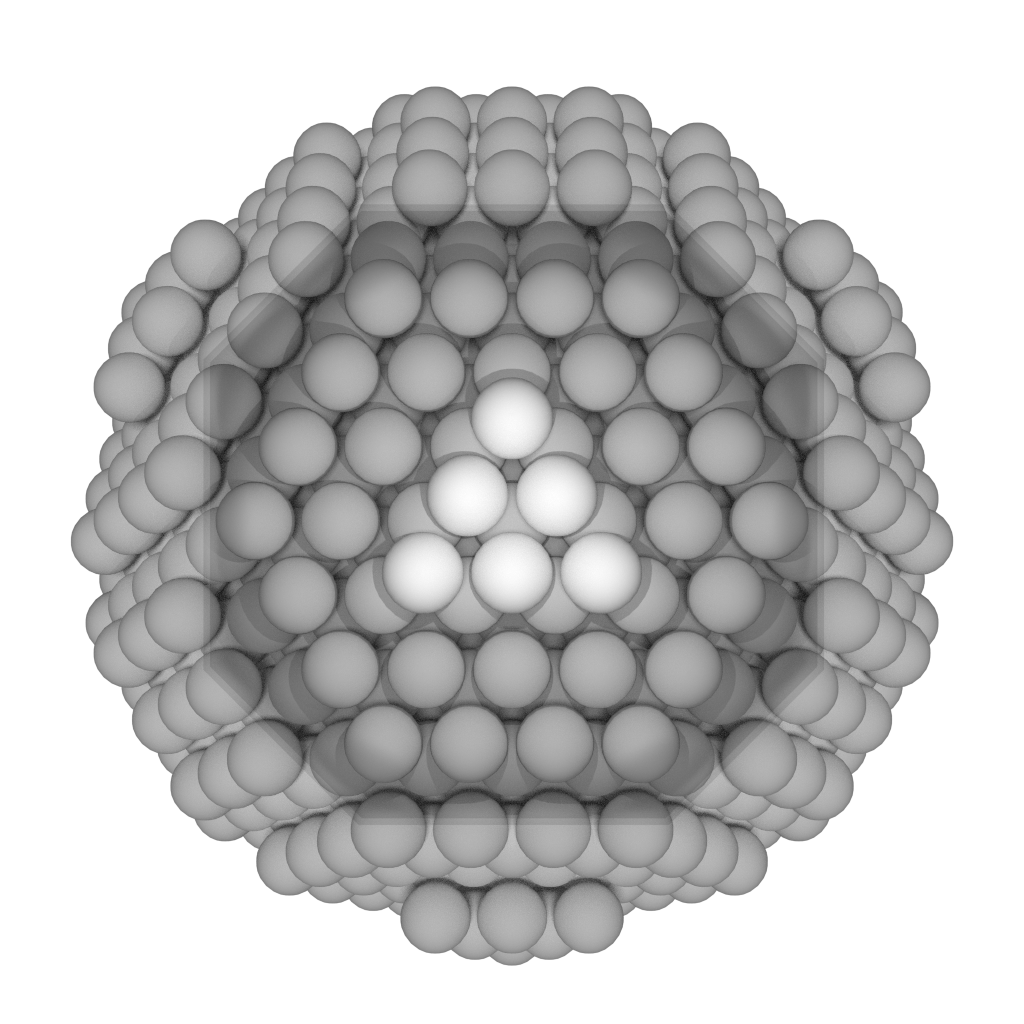
\includegraphics[width=0.3\textwidth]{./images/fcc-111-persp}} \quad
	\subfigure[(100)]{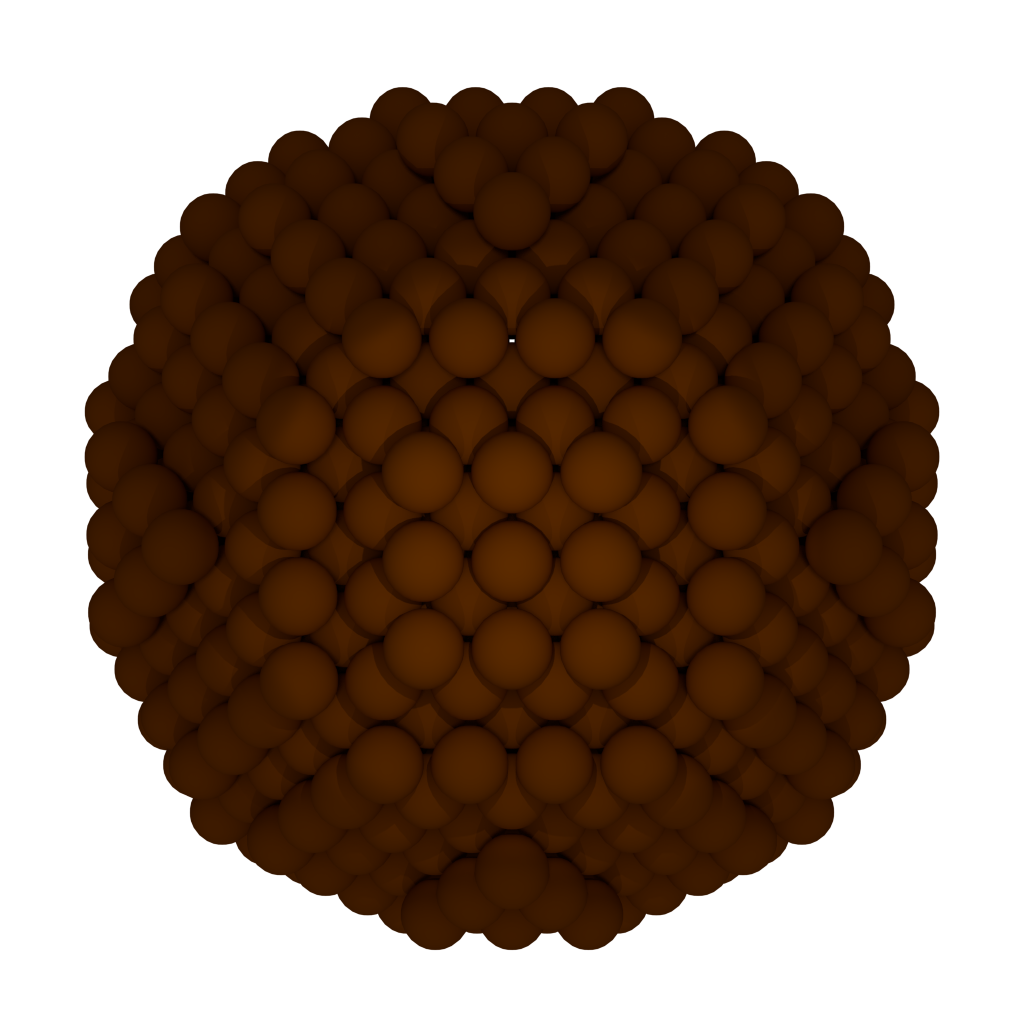
\includegraphics[width=0.3\textwidth]{./images/fcc-100-persp}}
%	\subfigure[(110)]{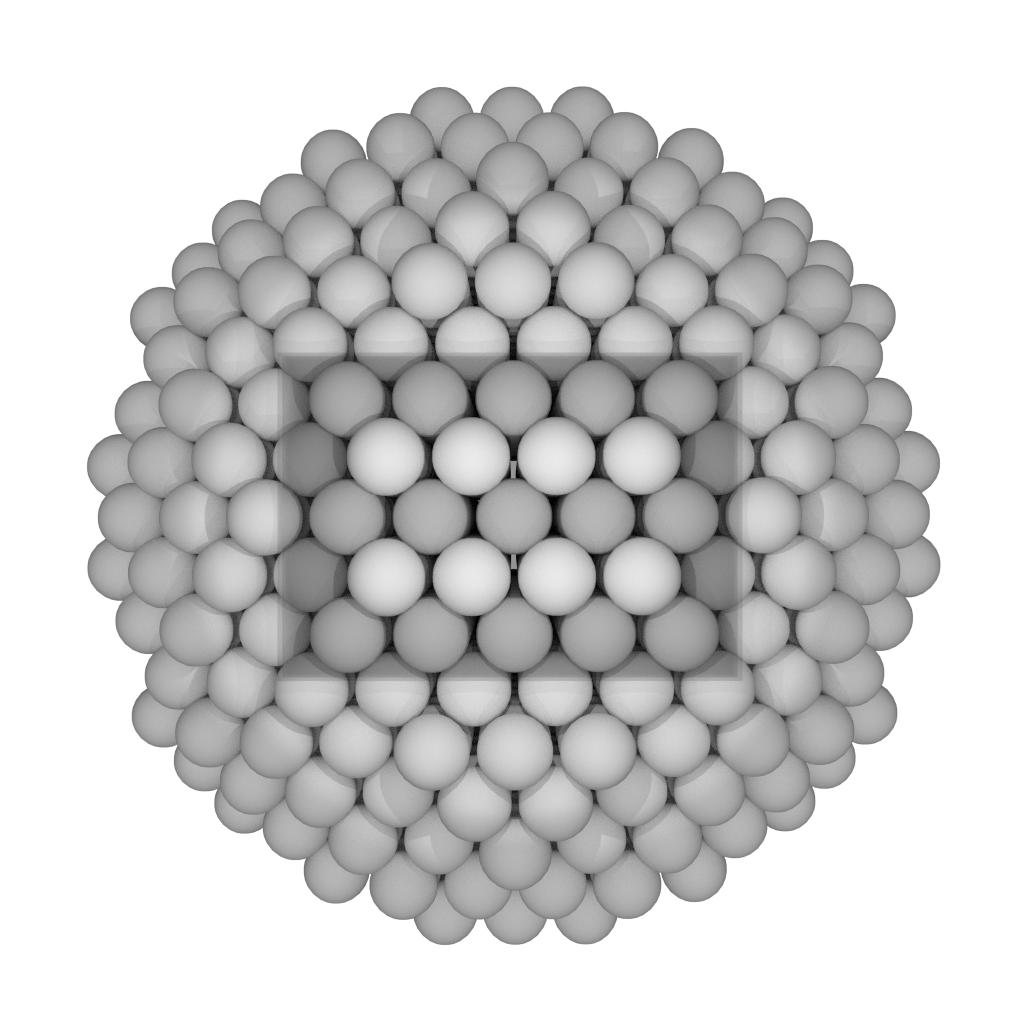
\includegraphics[width=0.3\textwidth]{./images/fcc-110-persp}}
	\caption{Identical crystalline balls in fcc lattice configuration. The surface termination is determined by the direction of the intersecting plane (parallel to the paper plane) relative to the lattice and forms (111) and (100) surfaces.}
	\label{fig:crystal-termination}
\end{figure}

The surface free energy increases from the (111) surface with increasing angle of the (hkl) planes of interest with $$\cos(\phi)=\frac{h+k+l}{\sqrt{3(h^2+k^2+l^2)}}$$ \cite{jian-min_calculation_2004}. Thus, the (111) surface is the one with lowest energy, followed by (110) and (100). For polycrystalline foils it is expected to observe the lowest energy facet more often than the less favorable (110) and (100) facet.

Due to the fact that dislocation lines move within the crystal in a well defined manner, one can determine the crystals orientation when dislocation lines and step edges show on the surface.

\textcolor{red}{\textbf{
For fcc crystals the orientation of dislocation lines occurs in the {111} plane in $<110>$ direction. Its Burgers vector is $\frac{a}{2}[110]$\cite{_dislocation-theory}. \underline{ADD INFO	FOR 100!!!}
Dense packed rows in fcc(111) are the following directions: $<\bar 1 01>$, $<01\bar 1>$, $<1\bar 1 0>$. The diagonals are found in the $<\bar 1 \bar 1 2>$ and $<1\bar 2 1>$ directions. \underline{ADD INFO	FOR 100!!!}
}}
 
 \subsection{Polycrystalline copper foils}
 
  As was mentioned before, clean, highly ordered surfaces are desirable to perform experiments on. In case a systems order and functionality does not heavily depend on the substrates crystalline properties, single crystals loose most of their unique selling point. Instead of choosing a expensive bulk single crystal, thin copper foils can catch up in production environments. The mass produced foils, although pure ($\geq \SI{99.999}{\percent}$), were never meant to be atomically flat and show considerable height variation.

\begin{wrapfigure}{O}{4cm}\centering
	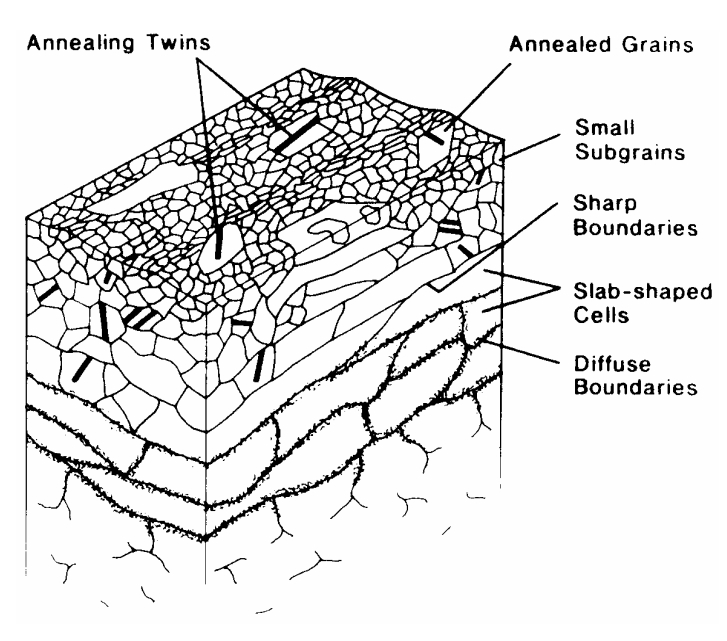
\includegraphics[height=40mm]{./images/grain-structure-copper-foil}
	\caption{Sketched bulk structure of a OFHC copper foil after abrasion with P1200 silicon carbide paper. Adopted from \cite{turley_nature_1981}}
	\label{fig:copper-foil-grains}
\end{wrapfigure}

 A representation of a mechanically polished copper surface can be seen in \autoref{fig:copper-foil-grains}. Here the layered structure is apparent and shows different sizes of grains. Small subgrains constitute the uppermost layers, while deeper lying layers consist of larger grains with grain boundaries becoming more and more diffuse with increasing distance to the surface. 
 
To overcome the limitation of small grain size and heavily corrugated surface, etching of the copper foil is performed as described in \autoref{sec:etching}.

     \subsection{\textit{h}-BN}
		In the last years, 2D materials with interesting properties were synthesized. One of it is hexagonal boron nitride. It is made up of the same number of nitrogen and boron atoms. They are arranged in an $\textnormal{sp}^2$-bonded honeycomb lattice so that each nitrogen is neighbored by boron atoms and vice versa. The ionic bond character between both is a direct result from the nitrogens larger electrochemical negativity, withdrawing electrons from the boron lattice site and making \textit{h}-BN an insulator with wide band gap of approximately \SI{6}{\eV}. \cite{watanabe_direct-bandgap_2004, cassabois_hexagonal_2016, blase_quasiparticle_1995} Free standing \textit{h}-BN is investigated with \textit{ab-initio} calculations \cite{han_effects_2014,mortazavi_investigation_2012,topsakal_first-principles_2009,peng_mechanical_2012}. Together with experiments \cite{paszkowicz_lattice_2002} a crystal lattice constant of $a_{\textit{h}-BN, RT}=\SI{2.504}{\angstrom}$ is derived.  It can be grown on a variety of metal surfaces.\cite{muller_epitaxial_2010,muller_one-dimensional_2008,guo_controllable_2012-4,siegel_heterogeneous_2017,schwarz_corrugation_2017,joshi_boron_2012,preobrajenski_monolayer_2005,vinogradov_one-dimensional_2012,farwick_zum_hagen_structure_2016,schulz_epitaxial_2014,Schulz_Templated_2013,gomez_diaz_hexagonal_2013,usachov_experimental_2012,orlando_epitaxial_2012,preobrajenski_monolayer_2007-1,preobrajenski_monolayer_2005,auwarter_synthesis_2004-1,auwarter_xpd_1999,nagashima_electronic_1995,corso_h-bn_2005,morscher_formation_2006,nagashima_electronic_1995,cavar_single_2008,muller_symmetry_2005,nagashima_electronic_1995,gomez_diaz_hexagonal_2013,dong_how_2010,brugger_reversible_2010,preobrajenski_monolayer_2007-1,berner_boron_2007,corso_boron_2004,brugger_comparison_2009,goriachko_self-assembly_2007}

 Depending on the substrates used, different lattice mismatches can be achieved. Many geometric corrugations can be achieved with increasing lattice mismatch and substrate-\textit{h}-BN interaction. Since this interaction is believed to have its origin in the partially filled d-states of the substrate,\textcolor{red}{\textbf{citation}} transition metal substrates are widely used. While substrates exist where the lattice constant are virtually identical (Ni: $\Delta \leq \SI{0.5}{\percent}$), other substrates show large mismatches (Ag(111): $\Delta \approx \SI{14}{\percent}$).

The growth of \textit{h}-BN on nearly lattice matched Ni(111) resulted in uniform commensurate layers. With increasing lattice mismatch, moir\'e patterns are formed on Pd and Pt. The stronger interaction of \textit{h}-BN and Rh(111) results in a corrugated nanomesh to be formed on the substrate.\textcolor{red}{\textbf{citation}} Even 1D structures are reported on Fe(110) \cite{vinogradov_one-dimensional_2012} and Cr(110) \cite{muller_one-dimensional_2008}. 

Here we consider \textit{h}-BN on Cu(111) as example system of self-limited growth and highlight most relevant insights reported in literature.\cite{joshi_boron_2012, schwarz_corrugation_2017, auwarter_hexagonal_2018}

\subsubsection{on Cu(111)}
%\begin{table}\centering
%	\caption{Lattice mismatches between \textit{h}-BN and several transition metal surfaces. The mismatch is given to describe the relative size of the \textit{h}-BN layer compared to the substrate, e.g. negative values indicate a larger lattice constant in the substrate bulk. Information adopted from \cite{_ptable}}
%	
%	\begin{tabular}{cccl}
%		Substrate 	& Mismatch [\%] 		& Electronic configuration \\ \hline
%		Ni(111)		& \SI{+0.4}{\percent} 	& [Ar] 3d8 4s2	\\
%		Cu(\left( 111)		& \SI{-1.9}{\percent} 	& [Ar] 3d10 4s1	\\	
%		 \\
%	\end{tabular}
%	\label{tab:h-BN-mismatch}
%\end{table}

	\paragraph{Stoichiometry}
	XPS measurements (see \autoref{fig:XPS-hbn-Cu111-martin}) show B\textit{1s} and N\textit{1s} components in a 1:1 ratio, indicating that the layer retains the precursor stoichiometry during growth, but all hydrogens are cleaved from the precursor prior to layer formation and desorp from the sample.\cite{Zhang_Two-dimensional_2017}
	
\begin{figure} \centering
	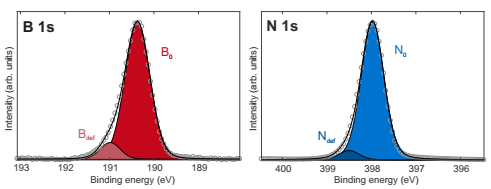
\includegraphics[width=0.7\textwidth]{./images/XPS-hbn-Cu111-martin}%
	\caption{XPS of a full ML \textit{h}-BN on Cu(111) grown with CVD. Fit components $B_0$ ($E_b=\SI{190.4}{\eV}$), $N_0$ ($E_b=\SI{398.0}{\eV}$) and $B_{def}$ ($E_b=\SI{191.0}{\eV}$) and $N_{def}$ ($E_b=\SI{398.5}{\eV}$) are assigned to pristine \textit{h}-BN layer and defective components respectively. Adopted from \cite{schwarz_assembly_2018}}
	\label{fig:XPS-hbn-Cu111-martin}
\end{figure}



	\paragraph{Moir\'e geometry}
	The properties of various moir\'e superstructures are well described in literature and Hermann gives a comprehensive overview in his paper.\cite{hermann_periodic_2012}\label{section:moire}
	
%	If lattice constants are equal like in the case of a graphene bilayer, the needed lattice mismatch occurs due to a rotation of the two layers. 
	A moir\'e is always present if an over layer shows a lattice mismatch with respect to the substrate. 
	
	For \textbf{isotropically scaled over layers} one can calculate the scaling factor $$p=\frac{R^{'}_{O1}}{R_{O1}}$$ which gives the size of the over layer lattice $R^{'}_{O1}$ in units of the substrate lattice $R_{O1}$. The moir\'e pattern shows the same bravais lattice type than the substrate\cite[10]{hermann_periodic_2012}. If moir\'e and ad layer lattice are aligned ($\alpha=0$\textdegree) the direction of moir\'e and substrate is aligned. If the over layer is isotropically scaled and not rotated, the period of the moir\'e calculates to $$a_{moir\'e}=\underbrace{\frac{p}{|p-1|}}_{\kappa}a_{substrate}$$
	With $a_{moir\'e}$ and $a_{substrate}$ are experimentally available, the ad layer lattice can be calculated with high precision (usually one order of magnitude more accurate than direct measurement of its period).\cite{farwick_zum_hagen_structure_2016}

Depending on the relative orientation of \textit{h}-BN and substrate the moir\'e period changes. Although large domains with uniform orientation can be grown on single crystal substrates (\autoref{fig:moire-STM-model}(a,c)), rotational domains exist(\autoref{fig:moire-STM-model}(b,d,e)).
The model representation nicely shows the change in moir\'e period when
\autoref{fig:moire-STM-model}(c) shows a case where the \textit{h}-BN ad layer has the same unit cell orientation than the copper. For a \textbf{scaled and rotated over layer} the angle between substrate and moir\'e ($\gamma$[rad]) scales with the angle between over layer and substrate ($\alpha$[rad]) as $\alpha=(1-p)\gamma$.
For rotated and isotropically scaled over layers, one can determine the $\alpha$ and $p$ from experimental observables $\gamma$(moir\'e angle to substrate) and $\kappa$(scaling factor) through relations $ \alpha=\arctan \left ( \frac{sin(\gamma)}{cos(\gamma)+\kappa} \right )\qquad p=\frac{\kappa}{\sqrt{1+\kappa^2+2\kappa cos(\gamma)}}$

\begin{figure} \centering
	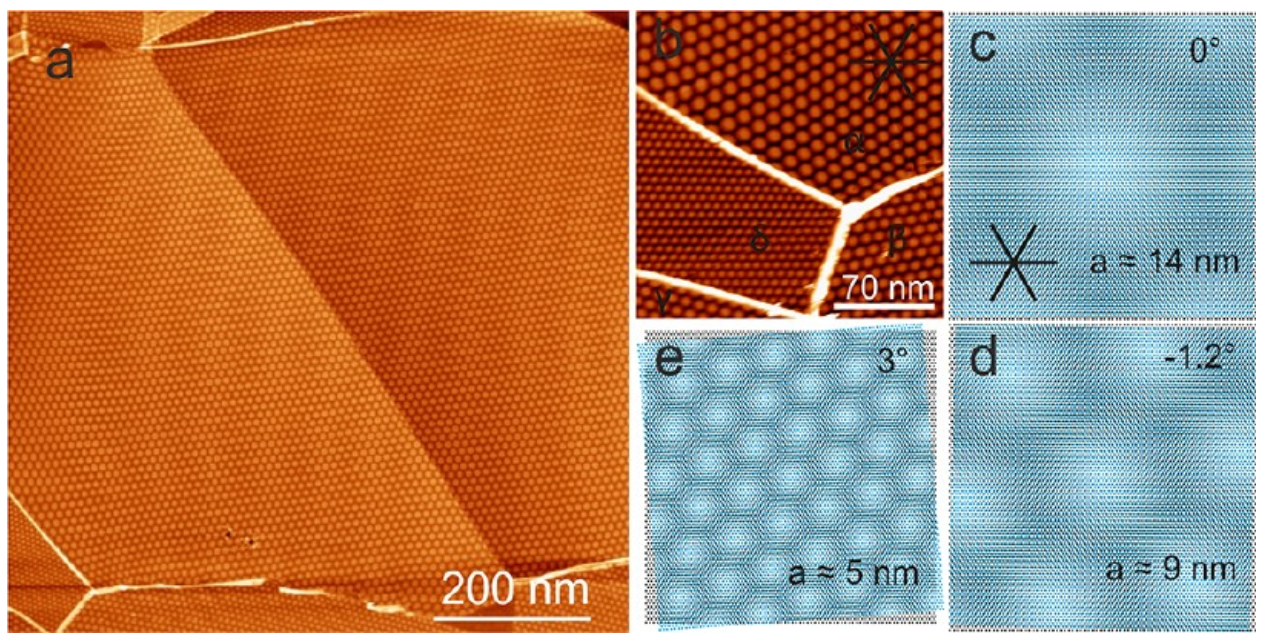
\includegraphics[width=0.5\textwidth]{./images/h-BN-cvd-cu111.png}%
\caption{(a) STM topography of \textit{h}-BN on Cu(111). Large domains with uniform orientation and moir\'e period are formed after CVD growth. (b) Different rotational domains are observed that show different moir\'e periods, reproduced by three models (c-e) where different \textit{h}-BN rotations are shown together with the resulting moir\'e periods a. Adopted from \cite{joshi_boron_2012}}
\label{fig:moire-STM-model}
\end{figure}

As mentioned above the orientation of the moir\'e superstructure is determined by the relative ad layer rotation alone, while its period is determined by lattice mismatch, too. This results in a variety of moir\'e superstructure orientations and periods, strongly related to the used substrate.
	
\paragraph{Periodic change in work function}
A direct result of the lattice mismatch between \textit{h}-BN and Cu(111) is the changing registry of ad layer atoms and substrate. The periodic modulation of B/N registry to the substrate atoms results in regions of stronger and weaker interaction between \textit{h}-BN and substrate and is the reason for the nano templating effect of \textit{h}-BN on many substrates.\textcolor{red}{\textbf{citation}} In the following some effects are discussed that lay the foundation for a nano patterning effect of \textit{h}-BN and its influence on the electronic structure of adsorbates.

While a first report in 2004 \cite{corso_boron_2004}, pointed to the formation of a complicated two layer structure, later experiments \cite{roth_chemical_2013, li_grain_2015} including ours \cite{joshi_boron_2012, schwarz_corrugation_2017} and others \textit{h}-BN/Cu(111) proofed a single layer of B \& N atoms in a regular hexagonal lattice. It evolved as well investigated system to perform experiments on. It could be shown that after CVD growth it adsorbs on Cu(111) as a flat layer. Due to its  lattice mismatch, "hill" regions  (corresponding to a $N_{top}B_{fcc}$ registry) and "valleys" (corresponding to a $N_{fcc}B_{hcp}$ registry) are formed. In these regions the work function is altered in opposite directions. While larger at the hill/pore regions, the work function reduces continuously to its lowest value in the valley/wire regions.\footnote{Please note that the notation is not uniform throughout the literature. Sometimes hills are referred to as pores and valley regions are denoted as wire regions.} 

Everywhere two regions with different work functions meet, local electrostatic fields arise to compensate for the vacuum level misalignment.

After growth of \textit{h}-BN the substrates over all work function is reduced [e.g. Rh: \SIrange{5.01}{3.07}{\eV} \cite{gomez_diaz_hexagonal_2013}. Therefor a dipole moment $\mu$ pointing from the the bulk to the surface is necessary, rather likely created by a negative charge transfer from the bulk into the ad layer.\cite{roman_periodic_2013}


\begin{figure} \centering
	\subfigure[Work function variation along \textit{h}-BN/Cu(111) moir\'e. (a) STM image showing the \textit{h}-BN moir\'e with a periodicity of 8.4 nm. Scan parameter: $U_b= 4.0 V, I_t= 40 pA$. (b)	Field emission resonances acquired along the black dotted line in a) revealing a variation of the peak positions. (c) Work  function  differences  between bright  (“hill”/pore)  and  dark  (“valley”/wire)  regions obtained  from  the  dI/dV curves  of  the  field emission  resonances  displayed  in  b). Adopted from \cite{schwarz_corrugation_2017}]{
		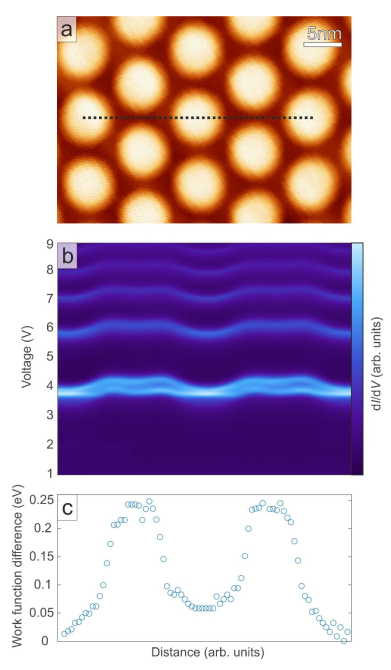
\includegraphics[width=5cm]{./images/h-BN-Cu(111)-wf-change}
	\label{fig:h-BN-Cu(111)-wf-change-I}
		} \quad
	\subfigure[Position dependent energy level alignment of $NC-Ph_4-CN$ on \textit{h}-BN/Cu(111). Three spectra are compared, recorded on molecules at valley (blue) and hill positions (green). A spectrum of the bare Ag(111) is shown as reference. Taken from \cite{diss-joshi}]{
	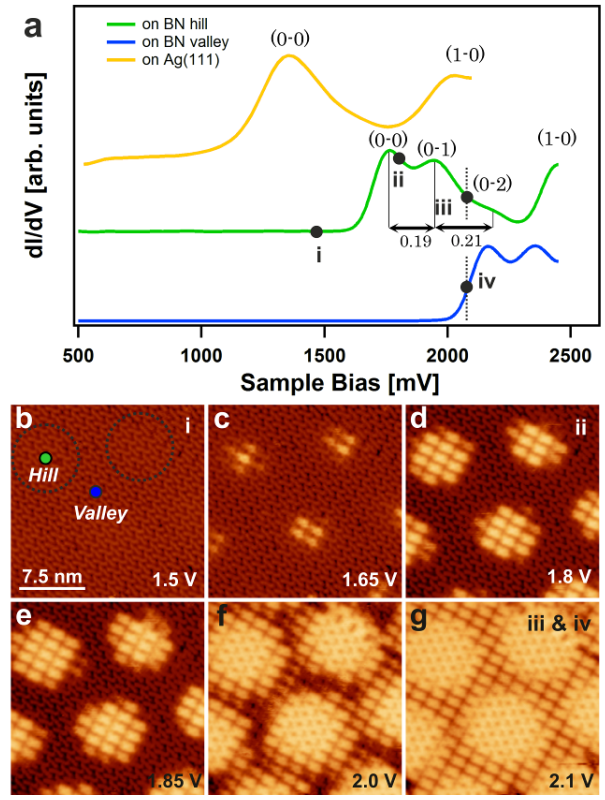
\includegraphics[width=6cm]{./images/h-BN-Cu(111)-wf-change-II}
	\label{fig:h-BN-Cu(111)-wf-change-II}
	}
	\label{fig:h-BN-Cu(111)-wf-change}
\end{figure}

\paragraph{Molecular adsorption and assembly}
\label{section:Mol-on-h-BN}
With changing work function, a lateral electric field emerges. For gr/Ru(0001) lateral dipole pointing from valley to pore sites arise.\cite{zhang_assembly_2011} It can be used to trap adsorbates with dipole moment along the field lines. This was shown for FePc and pentacene molecules on a graphene/Ru(0001) substrate. Here FePc molecules adsorp first on regions with high lateral dipole along top-fcc direction (valley), followed by regions with lower lateral dipole (on the hill). Pentacene molecules are trapped along the top-fcc direction, too.\cite{zhang_assembly_2011}  This general adsorption mechanism is applicable for other systems with periodic modulation of the work function.

\autoref{fig:h-BN-Cu(111)-wf-change} depicts the work function change measured with STS (Field emission resonances) indicating a similar modulation of the work function. In this theses TBP molecules (\autoref{section:TBP}) and helicene molecules (\autoref{section:helicene}) are used as sample molecules for specific adsorption site or orientation alignment.

It was shown that this moir\'e superstructure influences molecular assembly. 
\textcolor{red}{\textbf{Explain the Porphine adsorption on metal and on \textit{h}-BN}}

\begin{figure} \centering
	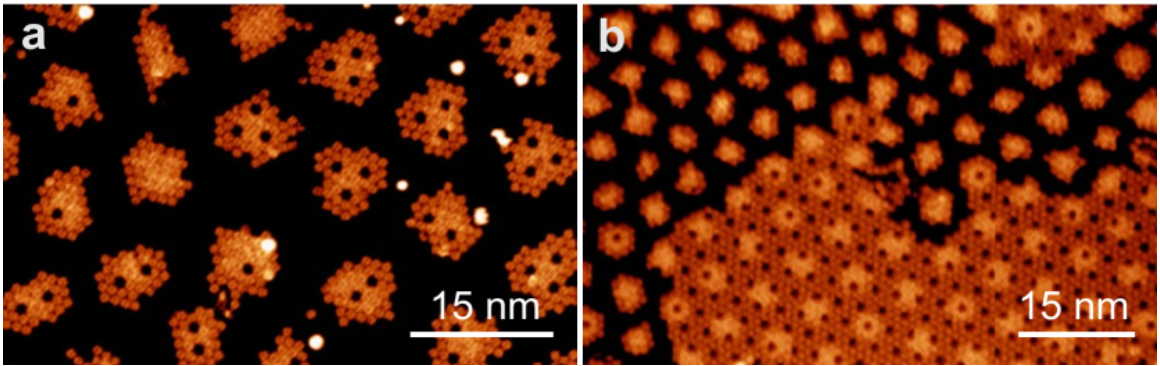
\includegraphics[width=0.7\textwidth]{./images/2H-P-hBN-Cu111-joshi}%
	\caption{STM topography of 2H-P adsorped on \textit{h}-BN/Cu(111). (a) A large moir\'e domain guides the formation of small 2H-P islands with off center vacancies. (b) High coverage overcomes the template effect of the \textit{h}-BN support. Adopted from \cite{diss-joshi}}
	\label{fig:2H-P-hBN-Cu111-joshi}
\end{figure}

\textbf{Molecules are electronically decoupled} when adsorped on a \textit{h}-BN spacer layer on top of a metal. The insulating \textit{h}-BN hinders the metal to influence molecular properties by charge transfer, image potentials etc.\textcolor{red}{\textbf{citation}}. As a result, molecular orbitals are unperturbed and can be imaged in STM/STS.

  \section{Sample preparation}
    \subsection{Etching copper foils}
Growing high quality \textit{h}-BN ad layers on polycrystalline copper foils requires a smooth surface, but as ordered Cu foils exhibit a root-mean-square (RMS) surface roughness $S_q$ of up to \SI{218}{\nm}\cite{bin_zhang_low-temperature_2012}. Steep, linear depressions, called striations are fabrication remnants due to the cold rolled foils and are observed on the surface\cite{kim_synthesis_2012-1}. Also some manufacturers apply a thin layer of chromium oxide for corrosion protection\cite{bin_zhang_low-temperature_2012}, that has to be removed prior \textit{h}-BN growth. A common procedure to reduce the roughness of a material is to mechanically polish the surface. When an even smaller RMS of height irregularities  
$$RMS\ \hat{=}\ S_q = \frac{1}{N}\sum_{n=1}^N\left(z_n-\bar{z}\right) \qquad z: \textnormal{heigth at point n}, \quad \bar{z} = \textnormal{mean heigth}$$ 
is needed, electrochemical polishing is an alternative.

\textcolor{red}{What are typical values for single crystal and foils? Check \cite{jinshan_electrochemical_2004} and experimental images in STM of Cu(111).}

The following gives a short introduction in chemical polishing as used for preparation of thin copper foils.\cite{antoine_polishing_1999, lilje_improved_2004, schulz_engeneering_2018}


\label{sec:etching}
\paragraph{Electrochemical cell}
The electrochemical cell, used to etch copper foils, is sketched in \autoref{fig:etching-setup}. A beaker is filled with etching solution and two electrodes are immersed. One electrode is the material to be polished (copper foil, working electrode), the other one is the counter electrode (copper in this case, counter electrode). Both are placed with \SI{3}{\centi \meter} apart and are oriented parallel. In this setup the working electrode has a surface of about \SI{1}{\square \centi \meter}, the counter electrode of about \SI{16}{\square \centi \meter}. The beaker is filled with etching solution until both electrodes are immersed.

An electric connection is made between working electrode (\SI{0}{\volt} < U < \SI{2}{\volt}) and the power supply. The counter electrode acts as ground. Both electrodes are fixed with alligator clamps to the wires. The current through the etchant depends on the applied potential and the etchant composition. The larger the current carried by the ionized copper atoms, the more material is transported from the working to the counter electrode.

\begin{figure}\centering
	\subfigure[Sketch of a typical setup used for electro polishing. A beaker is used to hold the aqueous cell medium. The copper foil and a counter electrode are immersed and connected a the + and - connections of a DC power supply. Image reproduced from \cite{stables_report_2008}]{
		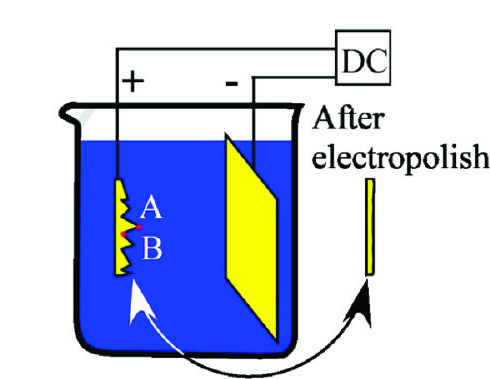
\includegraphics[width=0.4\textwidth]{./images/cm1028854-fig2-d}
		\label{fig:etching-setup}
	} \quad%
	\subfigure[Current-voltage characteristic indicating different phases in the ething and polishing process. While at low voltage etching is the dominant process, a polishing plateau is formed at intermediate voltages. Exceeding a threshold (cusp point) leads to increased formation of excess oxygen in the oxygen pitting regime. \cite{luo_effect_2011}]{
		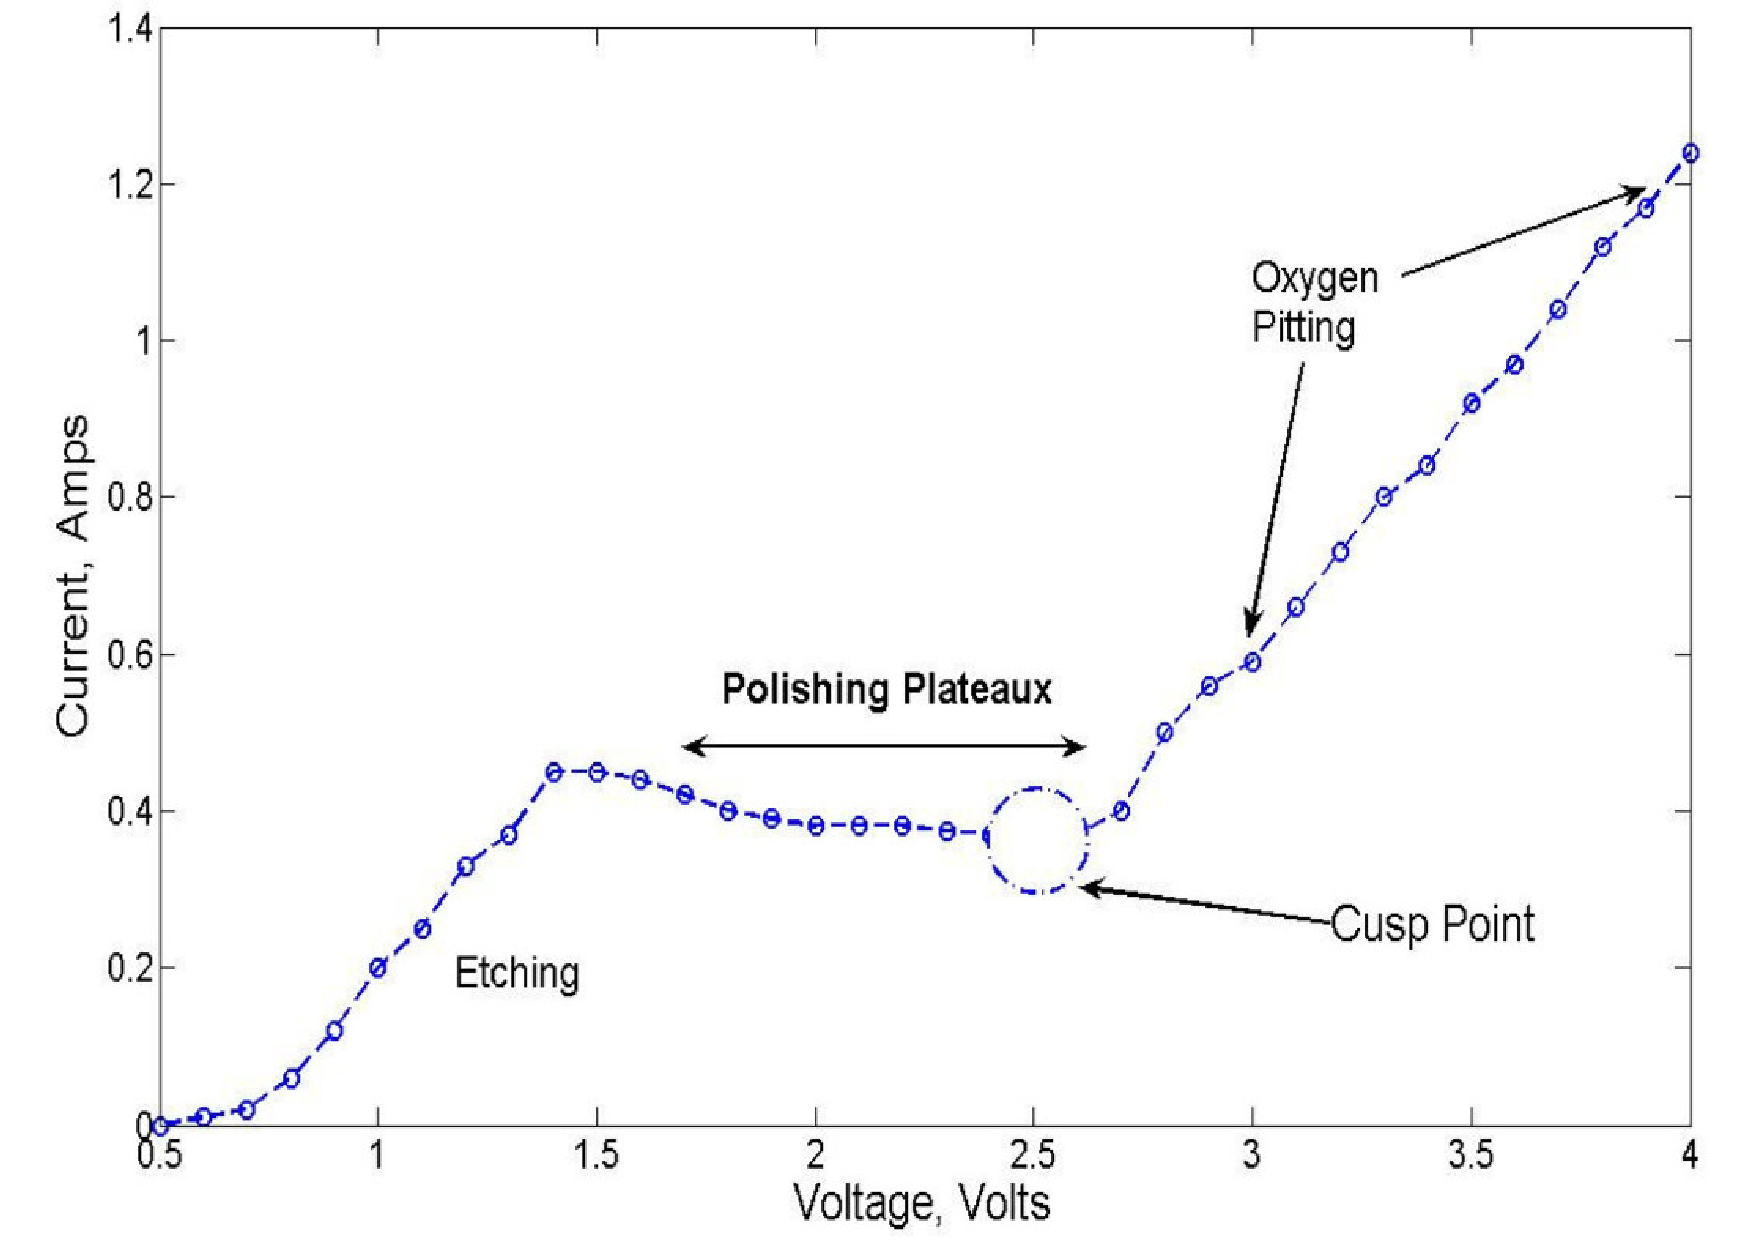
\includegraphics[width=0.4\textwidth]{./images/oxygen-pitting}
		\label{fig:oxygen-pitting}
	}
	\caption{Experimental setup and voltage characteristic used for electrochemical polishing of copper foils. \subref{fig:etching-setup} In the process the foil is connected as working electrode (+) and opposed by a counter electrode (-). Material is then transported from the working to the counter electrode resulting in a polished foil surface. \subref{fig:oxygen-pitting} Choosing proper voltage and current values within the polishing plateau is important for good results.}
	\label{fig:setup-and-characteristic}
\end{figure}

\paragraph{Aqueous etching solution}\index{electrochemical polishing}
Many different etching solutions are presented in literature, the most widely ones are summarized by Jinshan et al. in \cite{jinshan_electrochemical_2004}. Since the main goal is to achieve a flat surface, the resulting roughness of the surface is the most important parameter. 

Here two simple but efficient etching solutions that both result in a smooth surface and little etch pits are compared in \autoref{table:used-etching-solutions}. First, pure aqueous ortho-phospheric acid (\SI{85}{\percent}) was investigated as etchant \cite{jinshan_electrochemical_2004} with a anode-cathode potential of \SI{1.2}{\volt}. The limiting current is \SI{12}{\milli \ampere}. If now Ethylene-glycol (EG) (\SI{5}{\percent} of solutions volume) and deionized water (\SI{25}{\percent}) are added, the potential range to etch at remains the same, but the critical current is increased. Although the etching rate increases by a factor of 4, the resulting roughness remains the same \SI{5}{\nano \meter}, so foils etched with one of both recipes are of comparable quality. In contrast to etching recipes without EG where oxygen pitting is an issue (see \autoref{oxygen-pitting}) and more complex etching recipes (with reduced etching time but larger RMS) the chosen etchant composition (see \autoref{tab:composition-etching-solution-I}) is reported to give the best results.

\begin{table}\centering
	\caption{Used etching solutions (compare \cite[130]{jinshan_electrochemical_2004}). Note the change in the removal rate due to higher limiting currents in the solution after adding ethylene glycol to the solution.}
	\begin{tabular}{lcc}
		& I & II \\ \hline \hline
		$\SI{85}{\percent} H_3PO_4$ & 70 & 100 \\
		Ethylene-gylcol & 5 & 0 \\
		Deionized water & 25 & 0 \\ \hline
		Potential [\SI{}{\V}] & \multicolumn{2}{c}{\SI{1.2}{}} \\
		Current [\SI{}{\mA}] & 46 & 12\\
		Roughness [\SI{}{\nm}] & \multicolumn{2}{c}{\SI{5}{}} \\
		Removal rate [\SI{}{\micro\meter\per\minute}] & \SI{1,0}{} & \SI{0,26}{}\\
	\end{tabular}
	\label{table:used-etching-solutions}
\end{table}

\begin{table}
	\centering
	\caption{Volume and mass fractions for copper foil etching solution.}
	\begin{tabular}{lcccc}
		&unit	&$H_3PO_4$ (85\%)&	EG	&	$H_2O$	\\
		Dichte $\rho$   &[$g/cm^3$]	&	1.87	&	1.11	&	1.00	\\
%		$1/rho$		&[$cm^3/g$]	&	0.54	&	0.90	&	1.00	\\
		Anteil 		& \%		&	70	&	5	&	25	\\ \hline
		Menge gesamt    &[$cm^3$]	&		\multicolumn{3}{c}{150} 	\\
		Menge anteilig  &[$cm^3$]	&	105.00	&	7.50	&	37.50	\\
		Gewicht         &[g]		&	196.35	&	8.33	&	37.50	\\
	\end{tabular}
	\label{tab:composition-etching-solution-I}
\end{table}

\paragraph{Redox reaction}\index{electrochemical polishing!chemical reaction}

Electrons and atoms at the solid surface have higher energy states. Thus some of the atoms on the metal surface may lose electrons to form ions. These ions may also recombine with electrons and become atoms at another moment. Depending on the electronic structures, some metals (such as sodium) are easier than others (such as platinum) to ionize. Copper is relatively stable. Still, some of the surface atoms may be expected to ionize at a moment. The ionization process may be promoted when the metal is in touch with an aqueous solution because: 
\begin{itemize}
	\item Metal ions can not move in the metal electrode but can move through the solution, generating an electric current in solution when an potential is applied.
	\item Electrons can move freely in metal solid (electric current in a metal) but can not survive in solution because they will quickly recombine with positive ions
	\item Water dipoles and negative ions in solution may form a shell around the metal atom and drag the surface metal ions into the solution.
\end{itemize}

The electrode connected to the positive pole of the power supply is called anode, the one connected to the negative pole of the power supply is called cathode. When the applied voltage is high enough, electrons in the anode may be pumped out and the metal atoms on the anode surface will be oxidized (e.g., $Cu - 2e = Cu^{2+}$) and dissolved into the electrolyte solution. Under electrical field, the positive ions (cations) move to the cathode and negative ions (anions) move towards the anode. The cations may fetch electrons here and are reduced to neutral atoms (e.g., $Cu^{2-} + 2e = Cu$) at the cathode surface. Therefore, charge transfer between the two electrodes is carried out via the ion drift in the electrolyte and electron conduction in metal wire. When the coppper foil to be polished is connected to the anode, dissolution is processed at certain potential. Likewise, when the foil is connected to the cathode, it will result in deposition. For electro polishing of copper, the copper part to be polished is set to be anode while the cathode can be any conductive material (e.g. copper).

The critical potential at which the oxidation / reduction starts to occur is related to the standard redox potential for a specific anode material. The redox potential $E_O$ is a measure (in volts) of the electron affinity of a substance - its electro negativity - compared with hydrogen (which is set at \SI{0}{\volt}). Substances more strongly electronegative (i.e., capable of oxidizing or accepting electrons) than hydrogen have positive redox potentials (e.g., $Cu/Cu^{2+}$: $E_O = \SI{0.34}{\volt}$). Substances less electronegative (i.e., capable of reducing or giving up electrons) than hydrogen have negative redox potentials (e.g., $Cr^{3+}/Cr^{2+}$: $E_O = \SI{-1.07}{\volt}$)\cite{jinshan_electrochemical_2004}

\paragraph{Voltage-current-characteristic or polarization curve}
On a polycrystalline metal surface there are sites, such as defects and grain boundaries, where atoms are at higher energy states. In addition, due to arbitrary crystal orientation, there are different crystalline planes with different energy states of atoms on the electrode surface. Therefore, atoms at all these different sites and planes have different standard redox potential $E_O$, and as a result, have different dissolution rates.
%	 according to eq. \ref{dissolution-rate}. 
Such an anodic dissolution will not lead to polishing. Instead, a crystallographic etching is produced (reference [9, 33-35] within \cite{jinshan_electrochemical_2004}). This is true at lower current (or applied potential). This refers to the \textbf{etching regime} in \autoref{fig:oxygen-pitting} with $U<\SI{1.5}{\volt}$.
The plateau where the current remains almost constant with increasing voltage is referred to as \textbf{polishing plateau}. 
		
With continuing increase of applied potential, other reactions than Cu oxidation and reduction may occur and contribute to the increasing current. These reactions produce $H_2$ and $O_2$ bubbles, which occur at or reach the anode surface. This is known as \textbf{oxygen pitting}. Gas (oxygen or hydrogen) bubbles may block $Cu^{2+}$ ion transport and therefore terminate the electrochemical dissolution process on the area inside the bubbles. However, the residual solution on the surface area inside the bubbles may react with Cu atom and result in chemical etching. Depending on the chemical property of the electrolyte solution and the value of current density at which the electrochemical dissolution is occurring, the etching speed can be higher than the rate of electrochemical dissolution. In this case, pits will be produced on the anode and produce a rough surface. If etching does not occur inside the bubbles, or if its speed is slower than that of electrochemical dissolution process, the area inside the bubbles will remain and appears as protruding particles after the electrochemical dissolution process. In either case, a rough surface is produced. Approaches to reduce the effect of oxygen bubbling are done by altering the etching solution with different additives.

Overall, the values of the current plateau and the shape of a polarization curve depends on electrolyte solution, anode material, solution circulation, temperature, and the distance between anode and cathode. Of all the factors, the electrolyte is the most important one determining the polarization curve.

\paragraph{Leveling mechanisms}
Up to now, only the dissolution of copper surface atoms into solution and their deposition at the counter electrode was discussed. If the surface is polished evenly depends on several processes that are known as leveling mechanisms. First of all, the etching process relies on the fact that the current density (and thus the etching rate) is higher in protruding regions of the copper foil (Ohmic leveling). For an evenly wetted copper foil surface, protruding regions have less electrolyte solution between the electrodes. The lower electrical resistance causes a larger current density and thus larger dissolution rates at protruding regions.

Second, the surface geometry determines the shape of the electrostatic potential created at the working electrode. Convex regions at the surface have higher normal electric fields than concave ones, so that the force acting on a ionized copper surface atom is largest at protruding regions. Since the dissolution rate is proportional to the electric field strength, protrusions will be dissolved faster than cavities.\cite{jinshan_electrochemical_2004, Huo_Electrochemistry_2007, luo_effect_2011}

It was shown that best results are achieved with following points fulfilled.\cite{Huo_Electrochemical_2003}
\begin{itemize}
	\item The polarization curve shows a wide limiting current plateau (polishing plateau) with low limiting current.
	\item Etching is performed voltage regulated.
	\item Good circulation of the electrolyte solution to ensure even electro polishing.
	\item Prevent oxygen and hydrogen bubbles created in the etching process to reach the anode surface. Parallel aligned, vertical electrodes are preferred.
	\item Extremely close electrodes increase the effect of ohmic leveling, though gas bubbles reach the anode surface quicker.
\end{itemize}

\paragraph{After etching treatment and storage}
After etching, the samples are rinsed with deionized water to neutralize and remove the remaining etching solution. To seal the samples from ambient moisture and oxygen, they are stored in isopropanol.

%	\paragraph{Removed mass from working electrode}
%	``The current flow of every two electrons results in one copper atom dissolved on the anode and deposited on the cathode. Since $\SI{1}{\ampere}= \SI{1}{\coulomb \second}$, the charge of one electron $e = \SI{1.60218E16}{\coulomb}$, so the number of electrons (per second) in 1 A current is $N_e = \frac{I}{e}$; the number of copper atoms being oxidized or reduced $N_a= \frac{1}{2} N_e= \frac{I}{2e}$, the number of moles $N_m = \frac{N_a}{N_A} = \frac{I}{2eN_A}= \frac{I}{2F}$ where Avogadro's number $N_A = \SI{6.02214E23}{\per \mole}$. The weight of $N_m$ mole copper $W = N_m M = \frac{IM}{2 F}$ where M is the molecular weight of copper. Thats a volume, $V = W / d =\frac{IM}{2 F d}$ where d is the density of copper. Thus a current I produces a dissolution/deposition rate in thickness (\SI{}{\centi\meter \per \second}) \begin{equation} R_d=\frac{M}{2 FdA}I \label{dissolution-rate}\end{equation}
%	where A is the area of the electrode surface.
%	\cite[34]{jinshan_electrochemical_2004}

\subsection{Sample cleaning}
\label{sec:sample-cleaning}
Contaminations 
%in copper (Ag: \SI{0.8}{ppm}, Pb: \SI{0.3}{ppm}, Bi: \SI{0.8}{ppm}) and silver (Cu: \SI{2}{ppm}, Fe: \SI{2}{ppm}, Au: \SI{0.8}{ppm}, Ni: \SI{0.8}{ppm}) 
are removed by repeated sputter\footnote{$U_{accel}=$\SIrange{800}{1000}{\volt}, $T_{sample}\approx \SI{300}{\kelvin}$} and anneal cycles\footnote{Cu: $T_{sample}=\SI{750}{\celsius}$, Ag: $T_{sample}=\SI{450}{\celsius}$, Au\textbackslash Mica: $T_{sample}= 450$} in UHV. While sputter and anneal times are very similar for all substrates ($t_{sputter}\approx$ \SIrange{20}{30}{\minute} and $t_{anneal}\approx \SI{5}{\minute}$ respectively), the annealing temperature is chosen well below the melting point of the substrate but high enough to allow contamination segregation from the bulk to the surface and atomic reordering at the surface. Typical cool down temperatures $\leq 5 \frac{K}{s}$ result in a smooth, atomically flat surface with large terrace size. 

Before CVD growth of \textit{h}-BN on copper the last cleanaing cycle uses annealing temperature in the \textit{h}-BN growth regime to remove contaminations present at growth temperatures.

\subsection{\textit{h}-BN growth}
\label{sec:h-BN-growth}
\textit{h}-BN is grown by catalytic decomposition of the  precursor on hot copper substrates in UHV. Typical borazine partial pressures of $\SI{1e-7}{\milli \bar}$ and evaporation times of $\approx \SI{5}{\minute}$ are used to dose \SI{22}{\langmuir} while the sample is kept at \SI{750}{\celsius}. After dosage, the temperature is kept constant for another \SI{5}{\minute} to ensure complete transition of the precursor into the 2D \textit{h}-BN layer and self-healing of defects created at growth. The sample is cooled down with cooling rates $\leq 5 \frac{\SI{}{\kelvin}}{\SI{}{\second}}$ so that no wrinkles are observed at STM investigation temperatures of $\approx \SI{5}{\kelvin}$.

Borazine is used as chemical precursor. It is stored in an evacuated liquid cooler to maintain temperatures below \SI{5}{\celsius} and to ensure no water contaminants are present. Both, elevated temperature and water contaminants, cause the precursor to degenerate quickly in the storage to form boric acid $H_3BO_3$, ammonia $NH_3$ and hydrogen. Boric acid is a white, solid powder easily recognizable in the storage. A second indication of borazine decomposition is the smell of ammonia. The design can be found in \autoref{sec:borazine-cooler}.

\subsection{Molecule deposition}
\label{sec:molecule-deposition}
%%%%%%%%%%%%%%%%%%%%%%%%%%%%%%%%%%%%%%%%%%%%%%%%%%%%%%%%%%%%%%%%%%%%%%%%%%%%%%%%%%%%%%%%%%%
Molecules are sublimated in UHV by organic molecular beam epitaxy (OMBE). The two/four pocket evaporators resistively heat small quarz crucibles to the chosen temperature while the unused ones are water cooled ($T\leq \SI{20}{\celsius}$). Prior to deposition molecules undergo a degas procedure to remove unwanted chemicals from the powder. A shutter is used to choose the open pocket and allows for accurate timing of evaporation intervals.

\begin{table}\centering
	\caption{Evaporation and degas temperatures used for different molecules.}
	\begin{tabular}{ccrc}
		Name			& Configuration & Degas [\SI{}{\celsius}]	& Evaporate [\SI{}{\celsius}]	\\ \hline \hline 
		TPCN			& ---		& ---		& 490		\\ \hline 
		\multirow{3}{*}{TBP}	&single		& \SI{4}{\hour} @ \SI{200}{}& 390	\\
		&cis		& ---		& \SI{400}{\celsius}\\
		&trans		& \SI{4}{\hour} @ \SI{200}{} + \SI{1}{\hour} @ \SI{270}{}&\SI{370}{}\\ \hline 
		\multirow{4}{*}{pyrene} & \multirow{3}{*}{cis}		& \SI{2}{\hour} @ \SI{180}{}&	\multirow{3}{*}{250}	\\
		&&+ \SI{1}{\hour} @ \SI{200}{} + \SI{10}{\minute} @ \SI{235}{} 	&\\
		&&+ \SI{1}{\hour} @ \SI{220}{}&\\ 
		&trans		& \SI{1}{\hour} @ \SI{230}{}		&\SI{265}{}		\\ \hline
		\multirow{3}{*}{DCDB} & \multirow{3}{*}{---} & 1h @ \SIrange{100}{150}{}& \multirow{3}{*}{\SIrange{220}{240}{}}\\
		&&+\SI{10}{\minute} @ \SI{170}{} + \SI{25}{\minute} @ \SI{200}{} & \\
		&&+ \SI{40}{\minute} @ \SI{220}{}&\\
		\hline
		Helicene & --- & \textcolor{red}{\textbf{1h @ \SIrange{100}{150}{}}} & \\
	\end{tabular}
	\label{tab:molecule-temperatures}
\end{table}

\chapter{Epitaxial hexagonal boron nitride on copper foils}
%
\paragraph{Experiment realization}The first attempt to etch the Cu-foil was performed with the $5\%_{vol}$ EG, $25\%_{vol}\,H_2O$ filled up with phosphoric acid. The etching was performed in a \SI{200}{\ml} beaker, filled with \SI{150}{\ml} etching solution. The setup is as depicted in fig \ref{fig:etching-setup}. The potential was adjusted to be \SI{1.2}{\V}. The current through the solution changes and is typically highest when the etching process started. After some minutes, the foil starts to change. The reflectivity changes, making the foil - shiny before etching - a little dull. After some additional time the foil begins to reflect light better again. This is the moment where the etching process is interrupted. The time inside the etching solution depends on the handling - but was usually $\geq \SI{2}{\hour}$.\footnote{Since the perfect point to perform polishing varies in time a automated etching process has been developed \cite{palmieri_besides_2001}}

One has to be careful if reproducible results are needed. During the etching process (as more and more copper settles on the counter electrode), the current and therefore the etching rate decrease continuously. When the beaker is moved, some of the debris on the electrode changes (the electrode's) surrounding and the etching rate (limiting current) increases again. Front- and backside of the foil are suspect to different etching rates - at least the foil has different appearance on its sides. The back side is generally more flat, because the side facing the counter-electrode always shows some additional protrusions.

\paragraph{After etching treatment}
The foil is taken out and cleaned from remaining etchants with purified water first and isopropanol afterwards. Foils are be stored in ethanol to avoid oxidation. 

To further improve the quality of the foil, one can follow the documented recipe for annealing the foil in a $H_2$ atmosphere (\SI{10}{sscm}, \SI{1000}{\celsius}, 30min)\cite{kim_synthesis_2012} to increase the copper grain size and further smoothen the surface. 

So prepared foils are investigated in XPS (compare figure \ref{fig:xps-self-grown}) - (discussion of peaks can be found inside the text. Comparable experiments  are performed by \cite[8]{stables_report_2008}).

\paragraph{SEM}
After the etching process one foil is investigated in SEM. It was stored for one day in isopropanol and blown dry with nitrogen. 

Invented in the 1930's by Manfred von Ardenne\cite{ardenne_elektronen-rastermikroskop_1938}, Scanning electron microscopy (SEM)\index{SEM} is another versatile tool for the experimentalist. In contrast to (LT-)STM and AFM, SEM is capable of imaging huge areas of the sample within a very short time, which allows for a vast overview as well as good statistics. Magnifications reach up to 500k and above, illustrating even features in the order of \SI{1}{\nano \meter}.

As the name already discloses, SEM scans the surface with electrons. Their interaction with the material are diverse and some of them are explained in the following. While all effects are present in every measurement, not every microscope features detectors for all of these. While detectors for secondary electrons are standard equipment others may be not.

%\begin{itemize}
% \item \textbf{Secondary electrons (SE)} are produced in the bulk by the high energetic primary electon beam within close proximity to the surface. This is why SEMs offer a very good resolution of the surface itself.
%  \item \textbf{Backscattered electrons (BSE)} are elastically scattered primary electrons. The resolution of this mode is not as high for the secondary electrons. The intensity of the BSE depends strongly on the the atomic number Z of the specimen. It is useful for a complementary view, for example when chemical composition is of high interest.
%  Electron backscatter diffraction (EBSD) is used to achieve information on the crystallographic structure of a specimen.
% \item \textbf{Characteristic X-Rays} are used to identify the composition and measure the abundance of elements in the sample, too. See section \ref{sec:XPS} and figure \ref{fig:auger-core} therein for more details.
% \item \textbf{Cathodoluminescence (CL)} happens when electrons hit a material and exite photons. This effect is used in televesion screens where high energetic electrons are accelerated onto a screen containing phosphorus. There they distribute their energy with many others, some of those loose energy in form of photons which wavelenghts are within the visible spectrum. These light is called cathodoluminescence.
% \end{itemize}

The primary electrons are created with a filament. These often consist of tungsten (metal, high melting point, low work function). Alternatives are lanthanum hexaboride ($\textnormal{LB}_6$) - often used in LEED setups, too - or zirconium oxide.
Electrons are accelerated (typical energies are within \SIrange{1}{40}{\kilo \eV}) and focused on the specimen surface in a spot with few \si{nm} diameter with condenser lenses. Scanning the surface is achieved with coils that deflect the electron beam and therefore the actual scanning spot.

When the electrons hit the surface, they interact with the specimen in a small volume. The volume depends on the electron's energy, the atomic number Z of the specimen and the specimen's density. It is typically in the order of \SIrange{0.1}{5}{\micro \meter}.

Drawbacks:
\begin{itemize}
 \item[-] Sample has to be mounted $\rightarrow$ no in-situ measurement, surface alteration in between
 \item[-] Rather ``dirty'' vacuum $\rightarrow$ surface alteration while measuring
 \item[-] Measurement destroys sample $\rightarrow$ adsorbate build-up due to chemical reaction below e-beam
\end{itemize}



\begin{figure}[]
	\begin{center}
		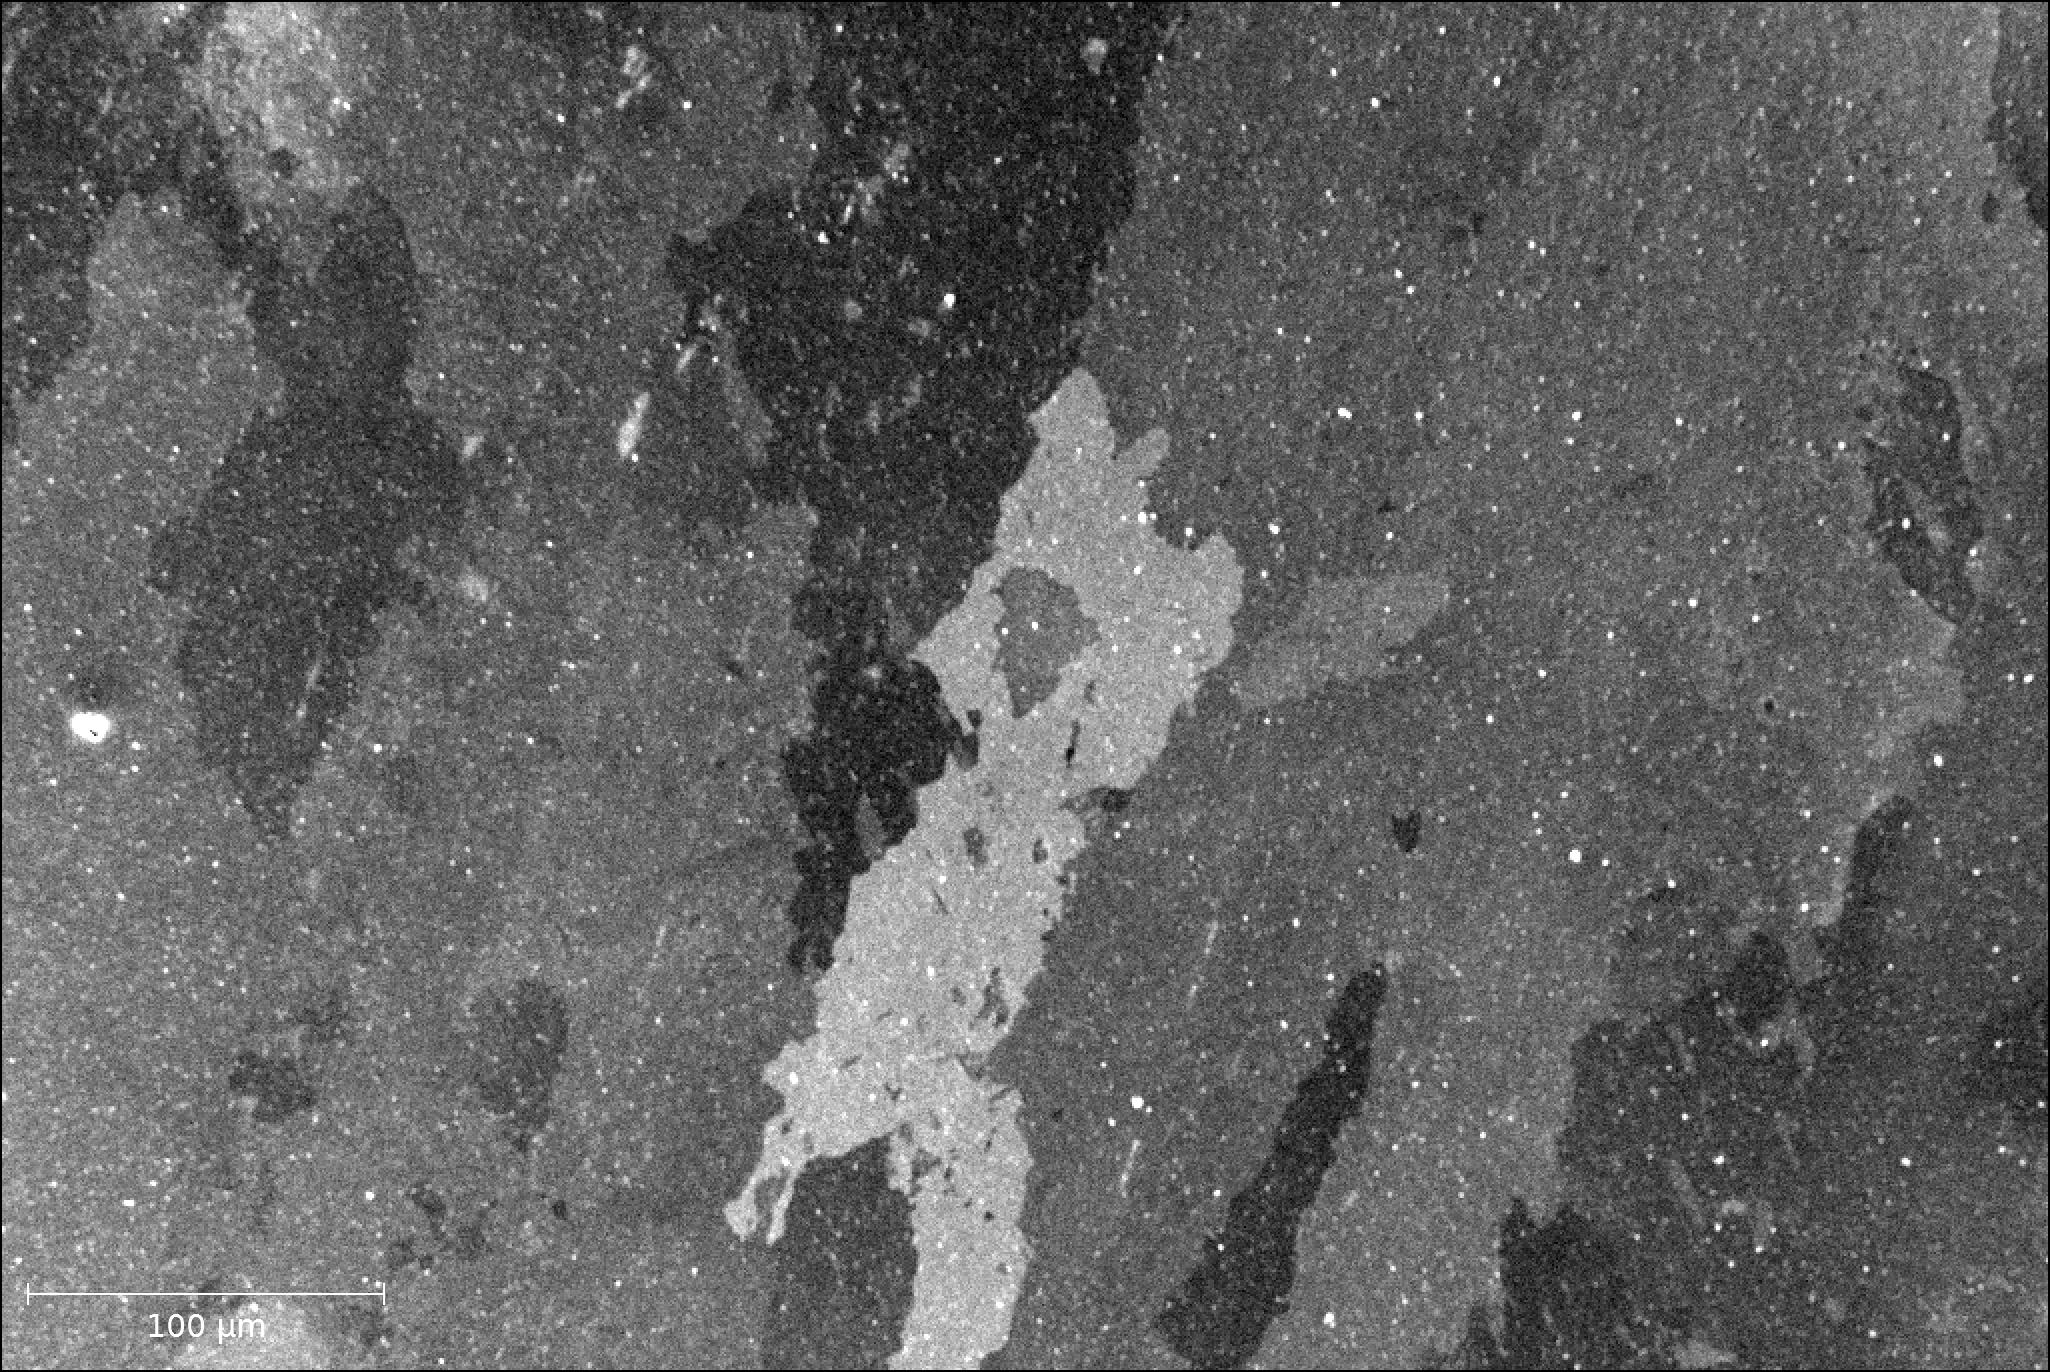
\includegraphics[height=6cm]{./images/Domenik_16031715.jpg}
		\includegraphics[height=6cm]{./images/Domenik_16031717.jpg}
	\end{center}
	\caption{SEM image of etched copper foil. Different contrast suggests different grain-orientation within the surface. a) Larger (\SI{570}{\micro \meter} x \SI{380}{\micro \meter}) image schowing the contrast of different grains in the copper-foil, b) zoom (\SI{18}{\micro \meter} x \SI{12}{\micro \meter})} to a area with two different contrasts and their border.
	\label{SEM-gb}
\end{figure}

One can see (\autoref{SEM-gb}) that the surface imaged in different intensities which correspond to the different orientation of the copper grains within the foil\cite{wu_effects_2015}. The grainsize may range from just a few \SI{}{\micro \meter} to several hundret \SI{}{\micro \meter} and in some cases even \SI{}{\milli \meter}. The grains are separated by grain boundaries. Large grains are preferred for growing graphene on copper foils because grain boundaries are subject to inhomogeneities within the graphene layer and provide a route for unwanted surface chemistry (copper oxidation for example). These effect can be also be used to highlight grain boundaries as shown in \cite{wu_effects_2015}.

Although not very rough, the copper foil shows surface variation. While some areas of the sample show some wavy surface, whereas other are much flatter and appear in a different intensity (\autoref{fig:SEM-surface}).

Neither estimation on the grainsize nor guesses for their absolute orientation have been done due to the lack of EBSD-data in the SEM setup.

\begin{figure}[]
	\begin{center}
		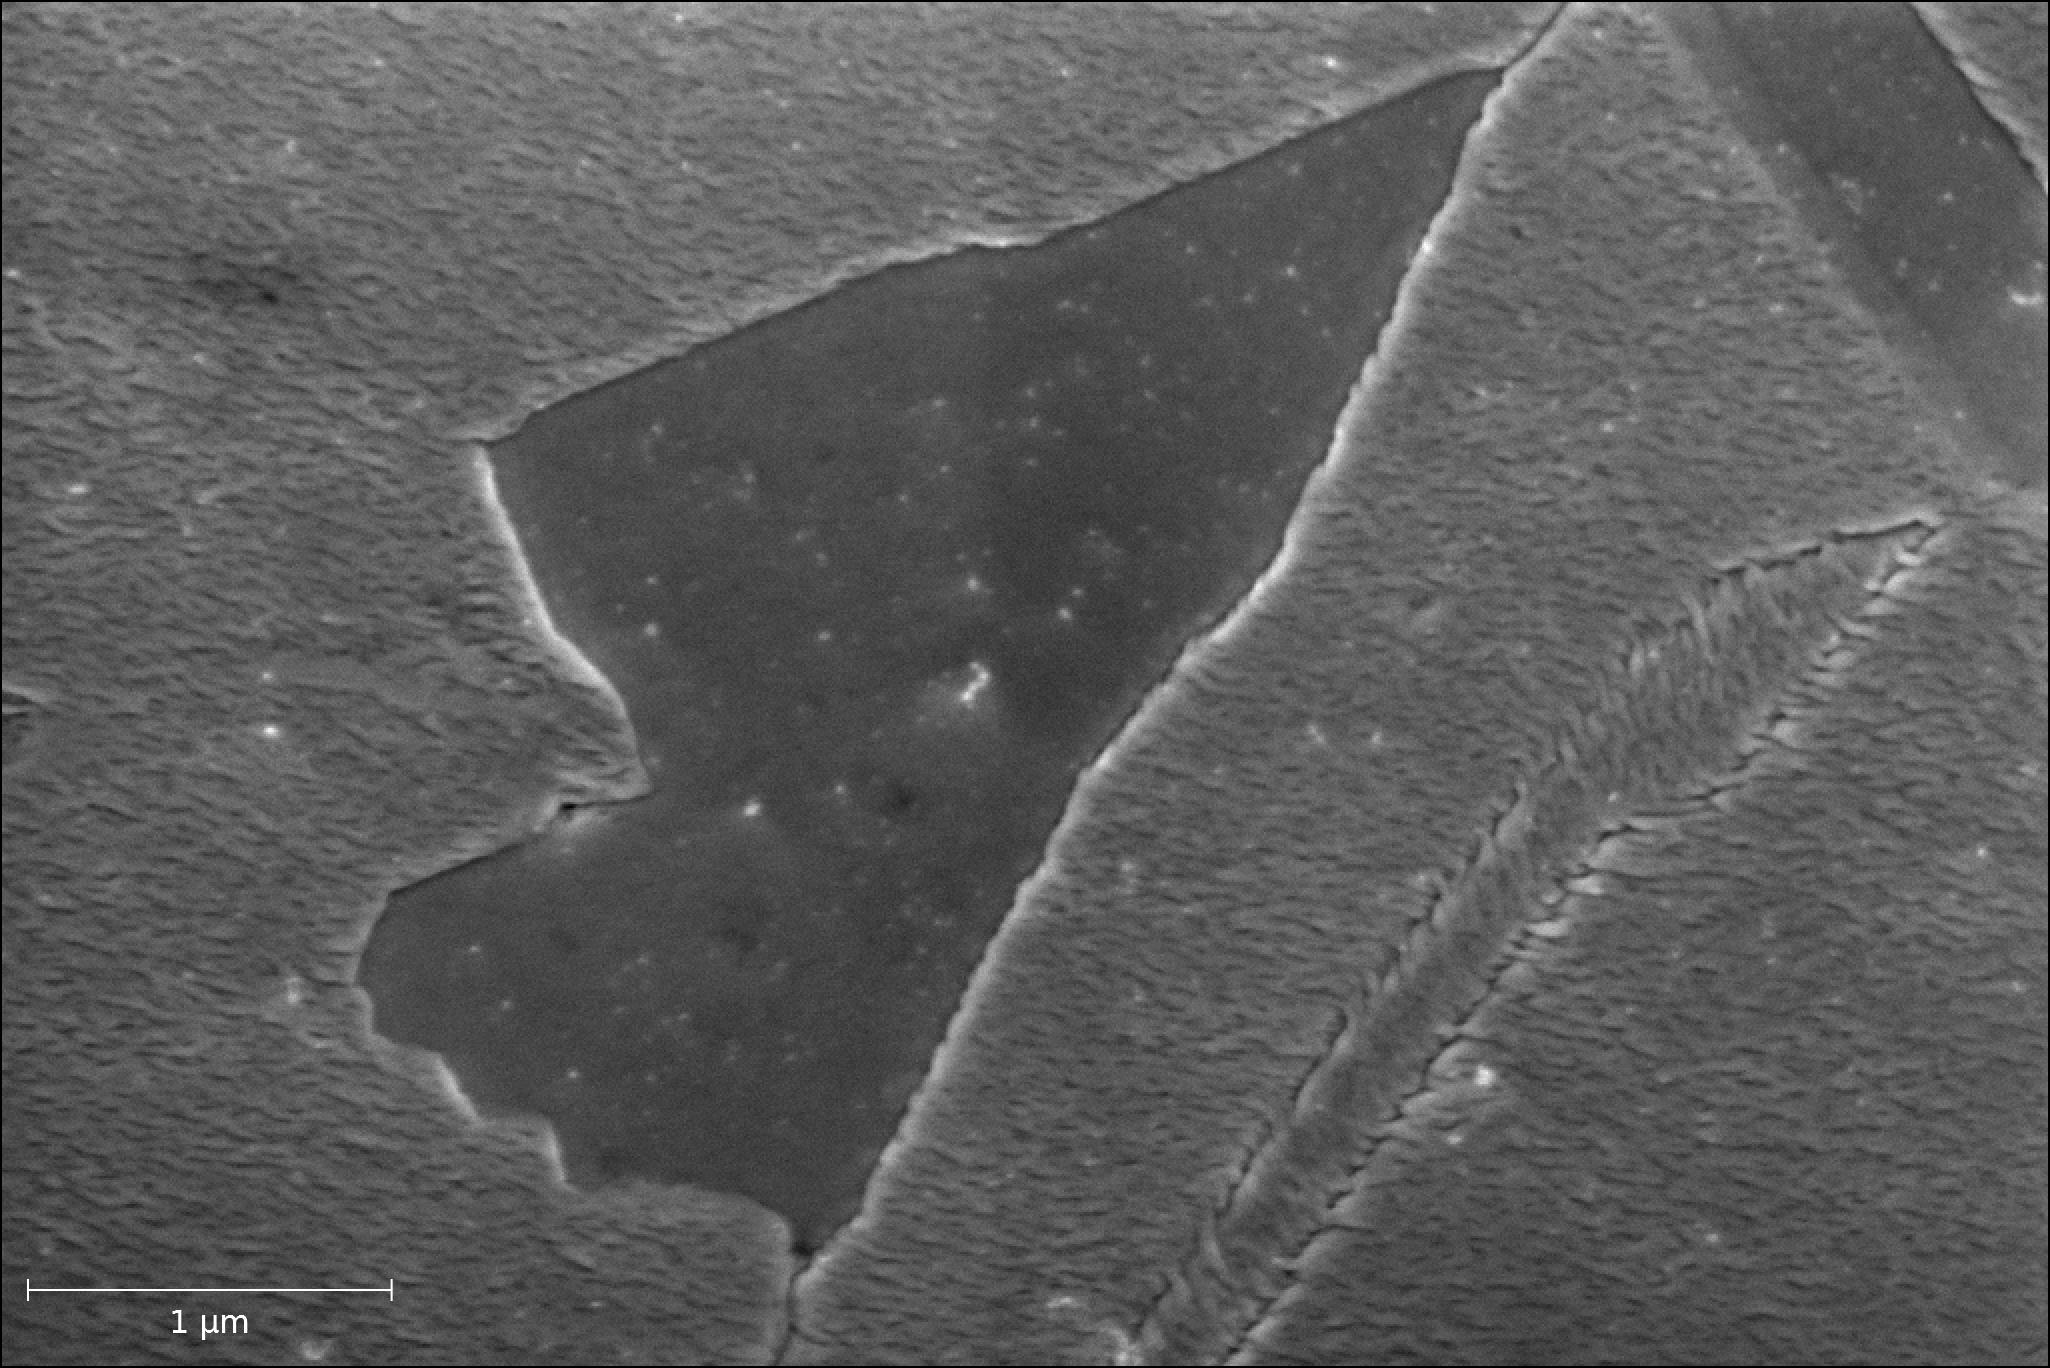
\includegraphics[height=6cm]{./images/Domenik_16031700.jpg}
		%\includegraphics[height=6cm]{../Daten/SEM/160317-Domenik/Domenik_16031717.jpg}
	\end{center}
	\caption{SEM image that shows different surface morphologies (\SI{5.6}{\micro \meter}x\SI{3.7}{\micro \meter})}
	\label{fig:SEM-surface}
\end{figure}

\paragraph{AFM}
\begin{figure}[] \centering
	\subfigure[RMS $\approx$\SI{13}{\nm}, contrast \SI{100}{\nm}]{
	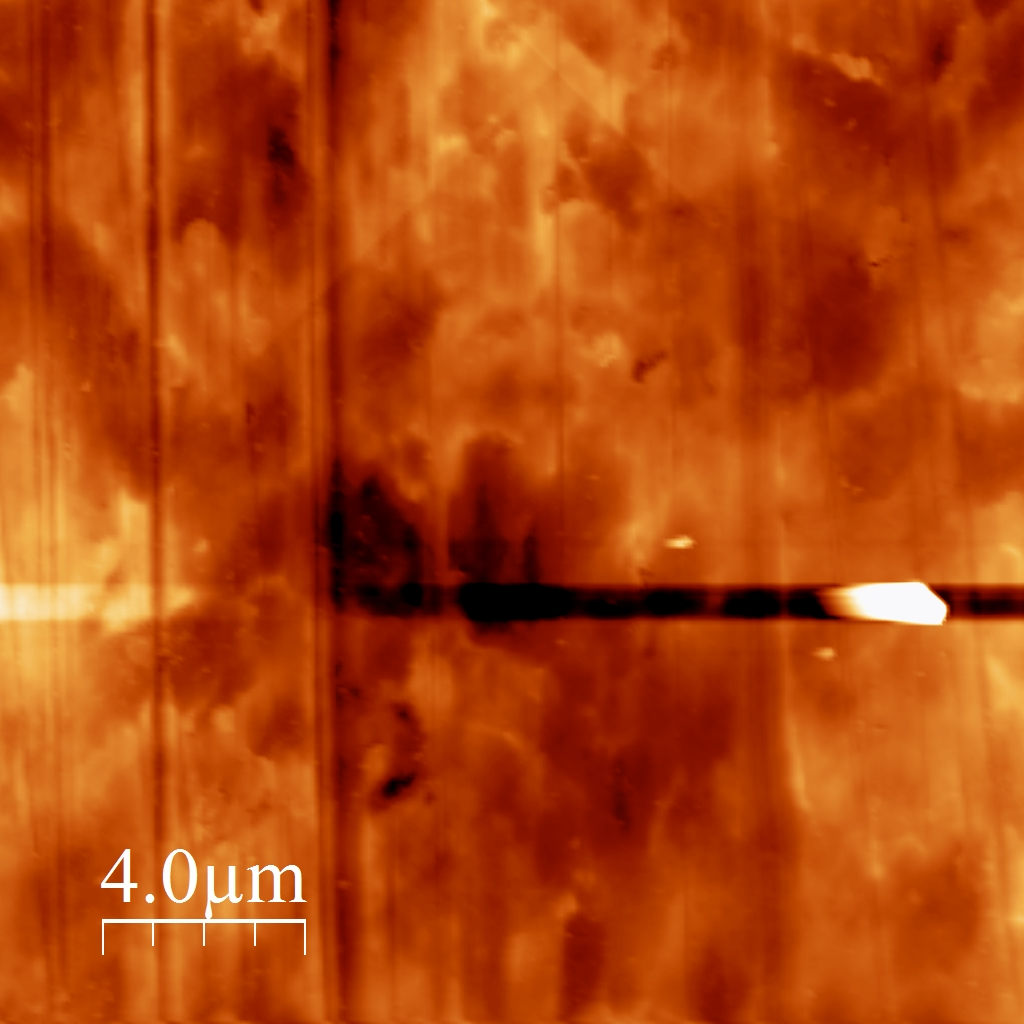
\includegraphics[width=0.4\textwidth]{./images/as_bought0000.jpg}
	}
	\subfigure[RMS $\approx$ RMS \SI{9}{\nm}, contrast \SI{70}{\nm} in the right image]{
	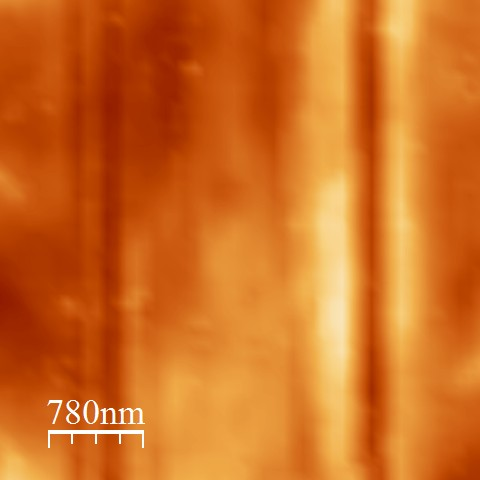
\includegraphics[width=0.4\textwidth]{./images/as_bought0001.jpg}
	}
	
	\caption{AFM image of the \SI{0.25}{\mm} copper foil as bought from alfa aesar.}
	\label{fig:foil-afm-as-bought}
\end{figure}

Figure \ref{fig:foil-afm-as-bought} shows the striations that stem from the production process (from top to buttom).
\begin{figure}[] \centering
	\subfigure[RMS $\approx$\SI{9}{\nm} in the left image, contrast \SI{100}{\nm}]{
	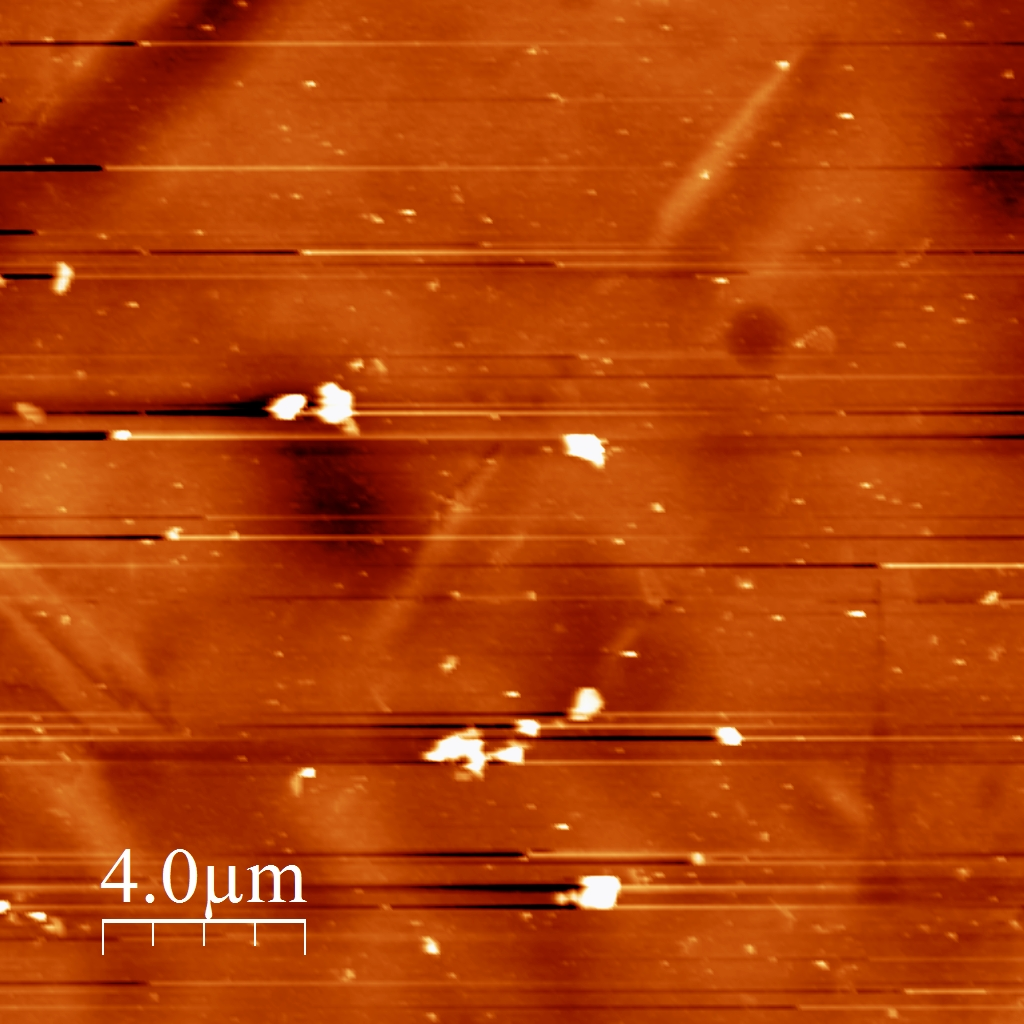
\includegraphics[width=0.4\textwidth]{./images/polished0000.jpg}
}
	\subfigure[RMS $\approx$\SI{3}{\nm} in the right image, contrast \SI{70}{\nm}]{
	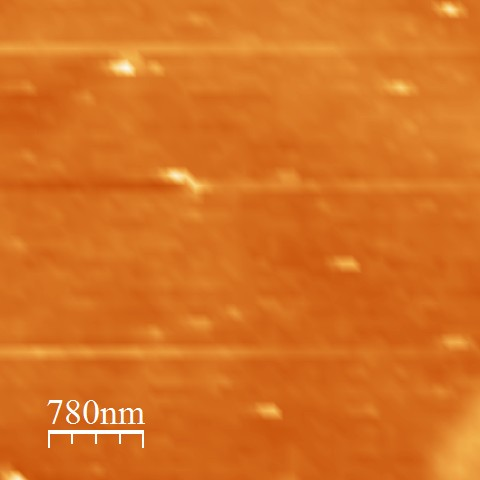
\includegraphics[width=0.4\textwidth]{./images/polished0001.jpg}
}
	\caption{AFM image of a copper foil polished 5h (according to table \ref{tab:used-etching-solution})}
	\label{fig:foil-afm-polished}
\end{figure}
After etching ($U=1.2V$,I=\SIrange{120}{250}{\mA}) for \SI{5}{\hour} in a solution (shown in table \ref{tab:used-etching-solution}) the striations have gone and the RMS value decreased by \SIrange{30}{45}{\percent} and an increase in foil quality is obvious even with bare eyes. Figure \ref{fig:foil-afm-as-bought} and \ref{fig:foil-afm-polished} show AFM images in the same size and contrast - before and after etching.
The circular hole is an effect of bubbles in the etching process where the bubble affects the rate of etching. The over all structure changes from a heterogenous sample height to a flat height contribution with only a little amount of defects. Those are sufficiently seperated in space to exhibit flat regions where the h-BN may grow unperturbated.



\paragraph{not done yet - maybe future?}
Some foil has been mechanically polished with 4k paper and several hours of Syton polishing. The roughness of these samples has been investigated also in AFM. These are comparable to the chemically polished ones, but are always slightly higher by $\approx 10\%$. Sometimes unwanted new scratches appear after mechanical polish.

\paragraph{STM}
The bought and chemically polished foils are mounted on a sample holder and loaded into the load lock. It is evacuated for \SIrange{2}{3}{\hour}, afterwards the valve is opened to the chamber. During transfer, no noteable increase in the base pressure is noted. The sample is put on the parking slot.

The sample was initially degassed with slowly increasing temperatures to remove adsorbates like $CO, CO_2$ and $H_2O$.

After some time of degassing, the sample was prepared with repeated sputter and anneal cycles. The annealing temperatures were increased up to \SI{800}{\degreeCelsius}. 
After that procedure, the sample was cooled down and observed in STM.

\begin{figure}[]
	\centering
	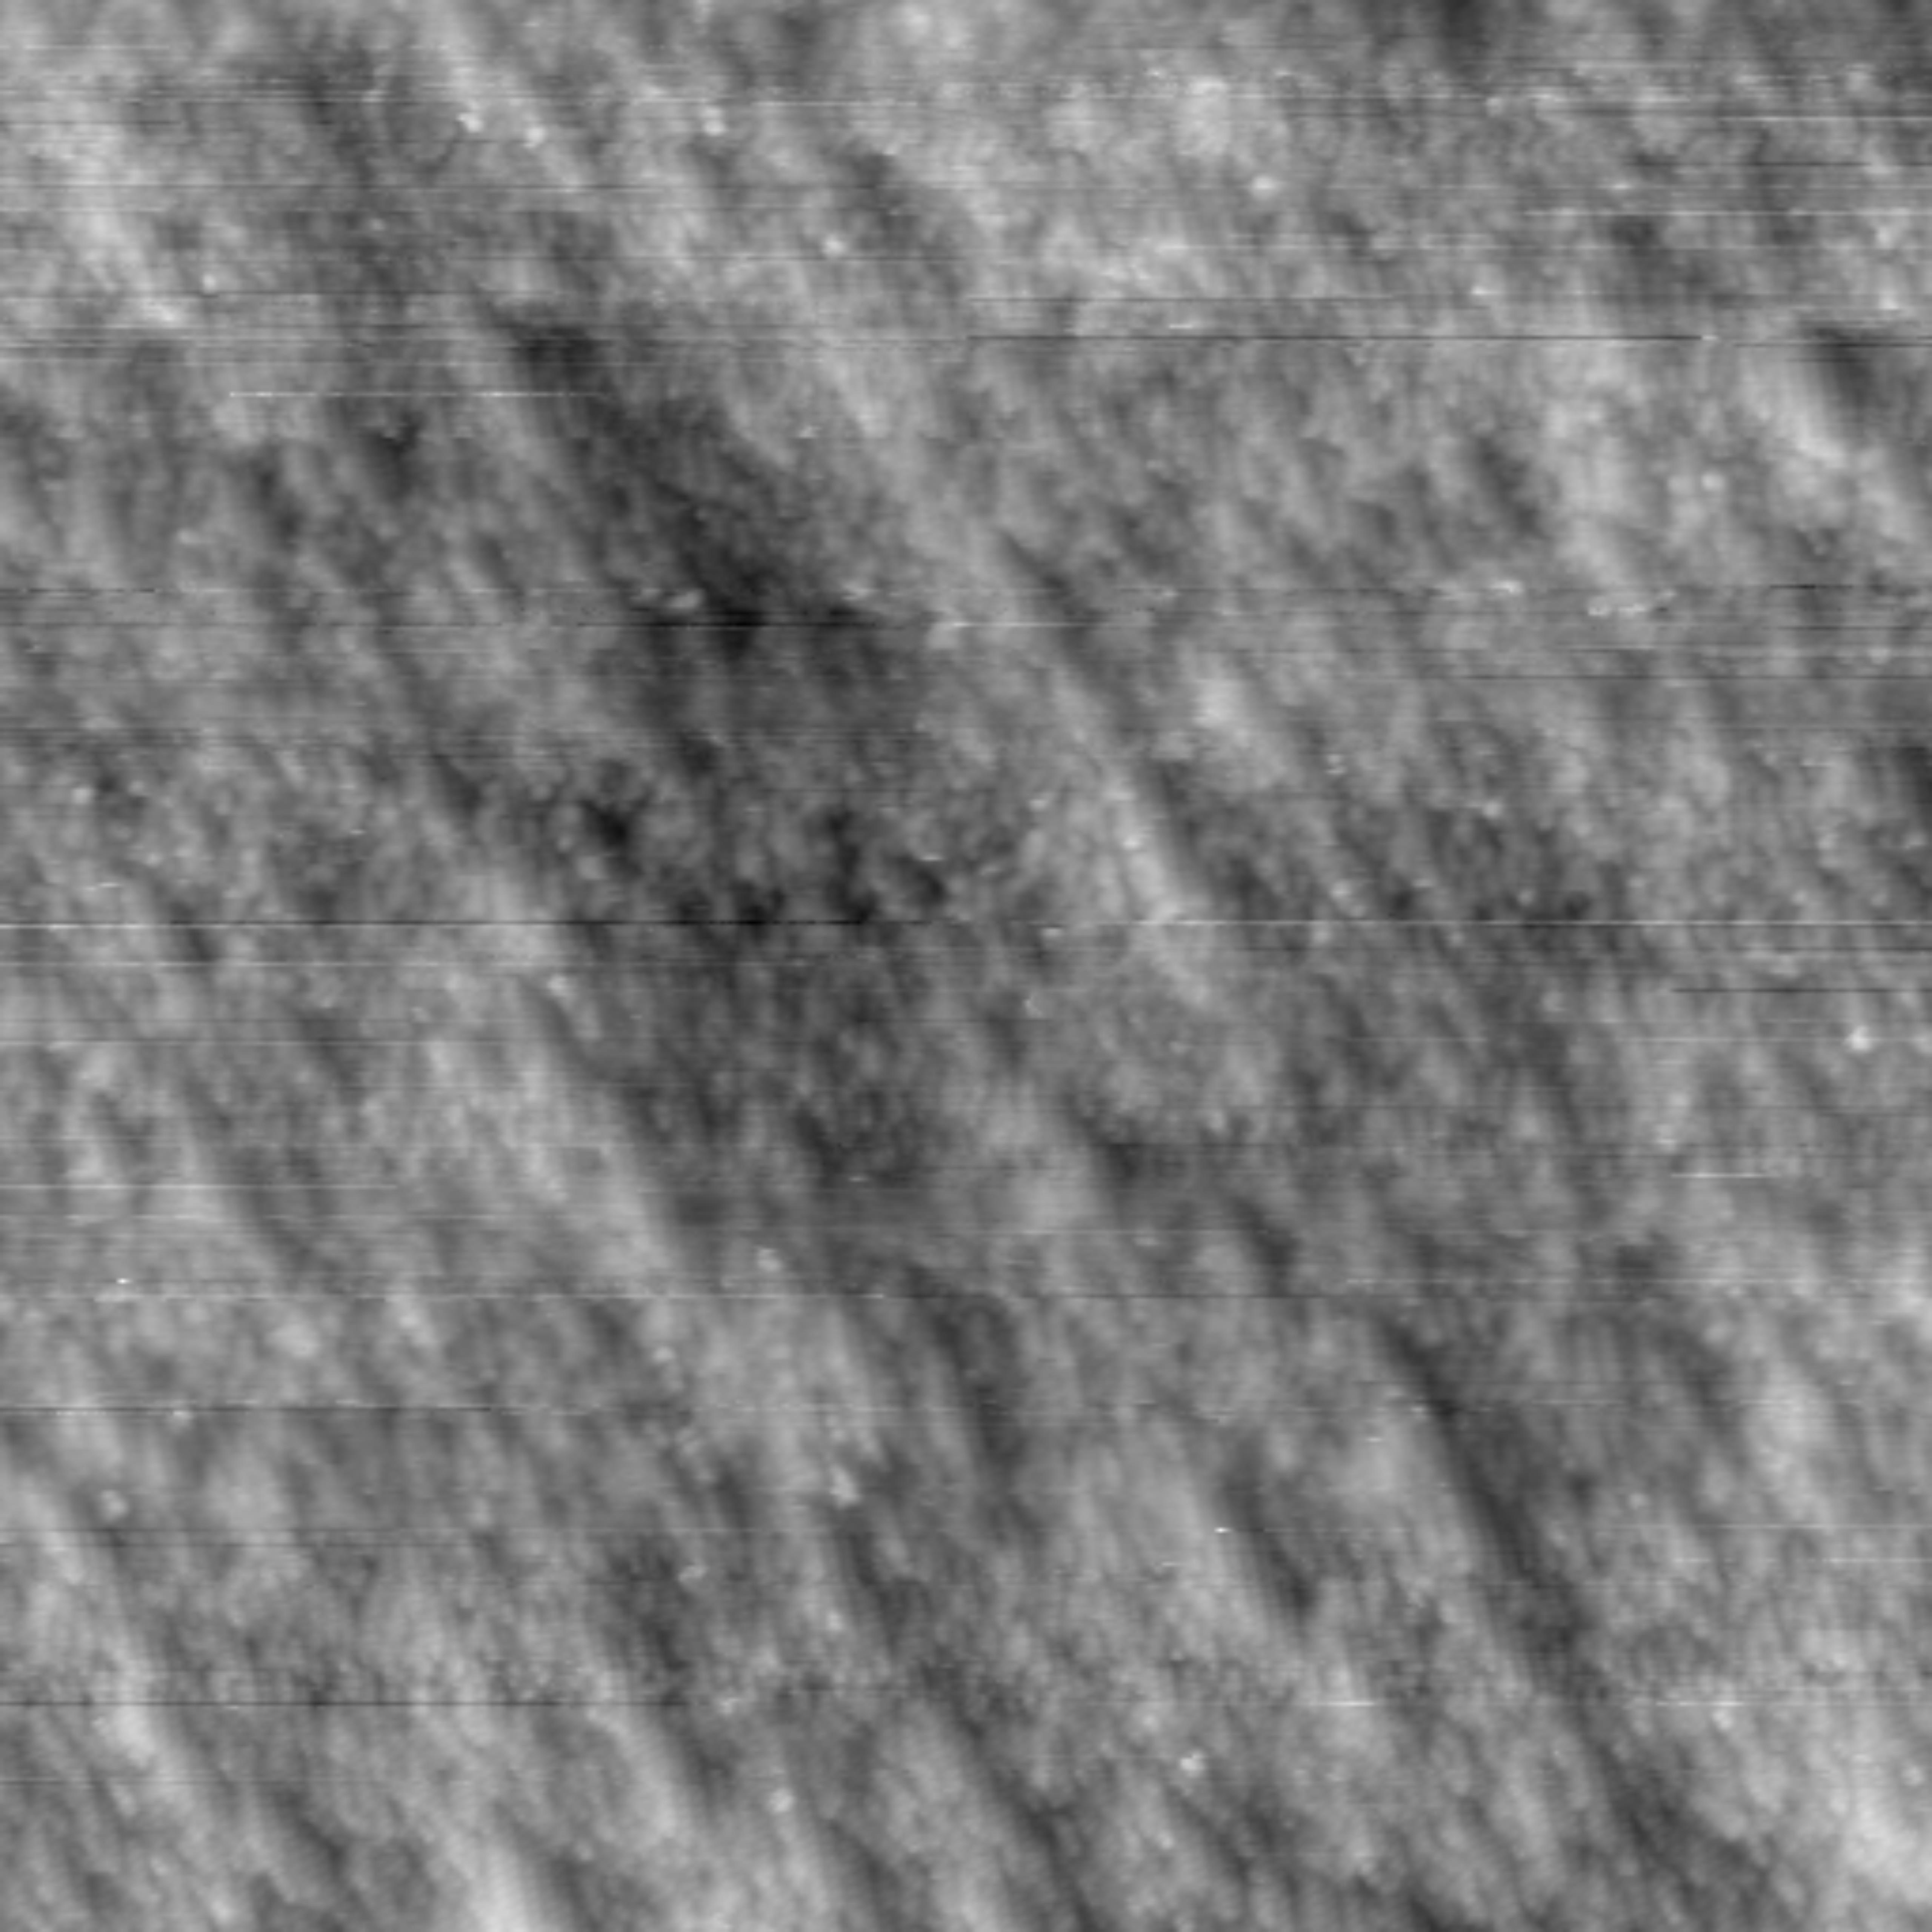
\includegraphics[width=0.5\textwidth]{./images/F150331-125720.jpg}
	\caption{Cu-foil after repeated sputtering and annealing cycles. A rather flat area is shown with no larger corrugation. The roughness is \SI{72}{\pico\meter}.}
	\label{fig:cu-foil-clean}
\end{figure}

A first look onto the sample shows a quite heterogeneous surface. While quite flat areas with a typical roughness of $\approx \SI{70}{\pico\meter}$ exist, areas with very large corrugations $\geq \SI{100}{nm}$ are hard to scan and bad places for \textit{h}-BN growth etc.
%\section{Motivation}
In this chapter copper foils are first chemically polished and prepared for investigation in SEM (p. \pageref{fig:SEM-gb}), AFM (p. \pageref{fig:foil-afm-as-bought}) and STM (p. \pageref{fig:cu-foil-clean-stm}). 

After CVD growth of \textit{h}-BN with borazine, foils are investigated in LT-STM (\autoref{fig:h-bn-overgrown-cu}) and XPS (compare \autoref{fig:xps-self-grown}). 

A commercially available \textit{h}-BN/Cu-foil is investigated in XPS after stepwise annealing to \SI{970}{\kelvin} (p. \pageref{sec:commercial-hBN-XPS}). 

At the end of the chapter (p. \pageref{sec:foil-use-case}) a use case shows that replacement of single crystals with polycrystalline foils is feasible for some applications.

%Comparable experiments  are performed by \cite[8]{stables_report_2008}). 

%%%%%%%%%%%%%%%%%%%%%%%%%%%%%
\FloatBarrier
%%%%%%%%%%%%%%%%%%%%%%%%%%%%%

\section{Pre-treatment of Cu-foils: Polishing}
	
	\paragraph{Experiment realization}The first attempt to etch the Cu-foil was performed with the $5\%_{vol}$ EG, $25\%_{vol}\,H_2O$ filled up with phosphoric acid. The etching was performed in a \SI{200}{\ml} beaker, filled with \SI{150}{\ml} etching solution. The potential was adjusted to be \SI{1.2}{\V} during the polishing process. The current through the solution changes and is typically highest when the polishing process started (\SI{120}{\milli \ampere}). 
	
After some minutes the foils reflectivity changes. The surface - shiny before etching - becomes hazy. After some more time the foils reflectivity improves again. 
	
	The time spend for polishing depends on the handling (like shaking the beaker or moving the foil in the solution). When no visual change to the surface is observed the etching process is interrupted.%\footnote{Since the perfect voltage/current to perform polishing varies in time a automated etching process has been developed. \cite{palmieri_besides_2001}}
	
During the etching process, as more and more copper settles on the counter electrode, the current and therefore the etching rate decreases continuously. When the beaker is moved, some of the debris on the electrode changes the electrode's surrounding and the etching rate (limiting current) increases again. 
	
	Front- and backside of the foil are suspect to different etching processes. The back side is generally more flat, the side facing the counter electrode always shows some additional protrusions.

The foil is cleaned from remaining etchants with purified water first and isopropyl alcohol afterwards in which they are stored in to avoid degradation under moist, oxygen rich ambient conditions. 
	
%%%%%%%%%%%%%%%%%%%%%%%%%%%%%
\FloatBarrier
%%%%%%%%%%%%%%%%%%%%%%%%%%%%%	

\subsection{RT-AFM}
	\label{sec:foil-AFM}
	To investigate the sample roughness for as-bought and polished foils, AFM measurements are done under ambient conditions and shown in \autoref{fig:foil-bought-afm}.
	
	\begin{figure}\centering
		\subfigure[Before etching]{
			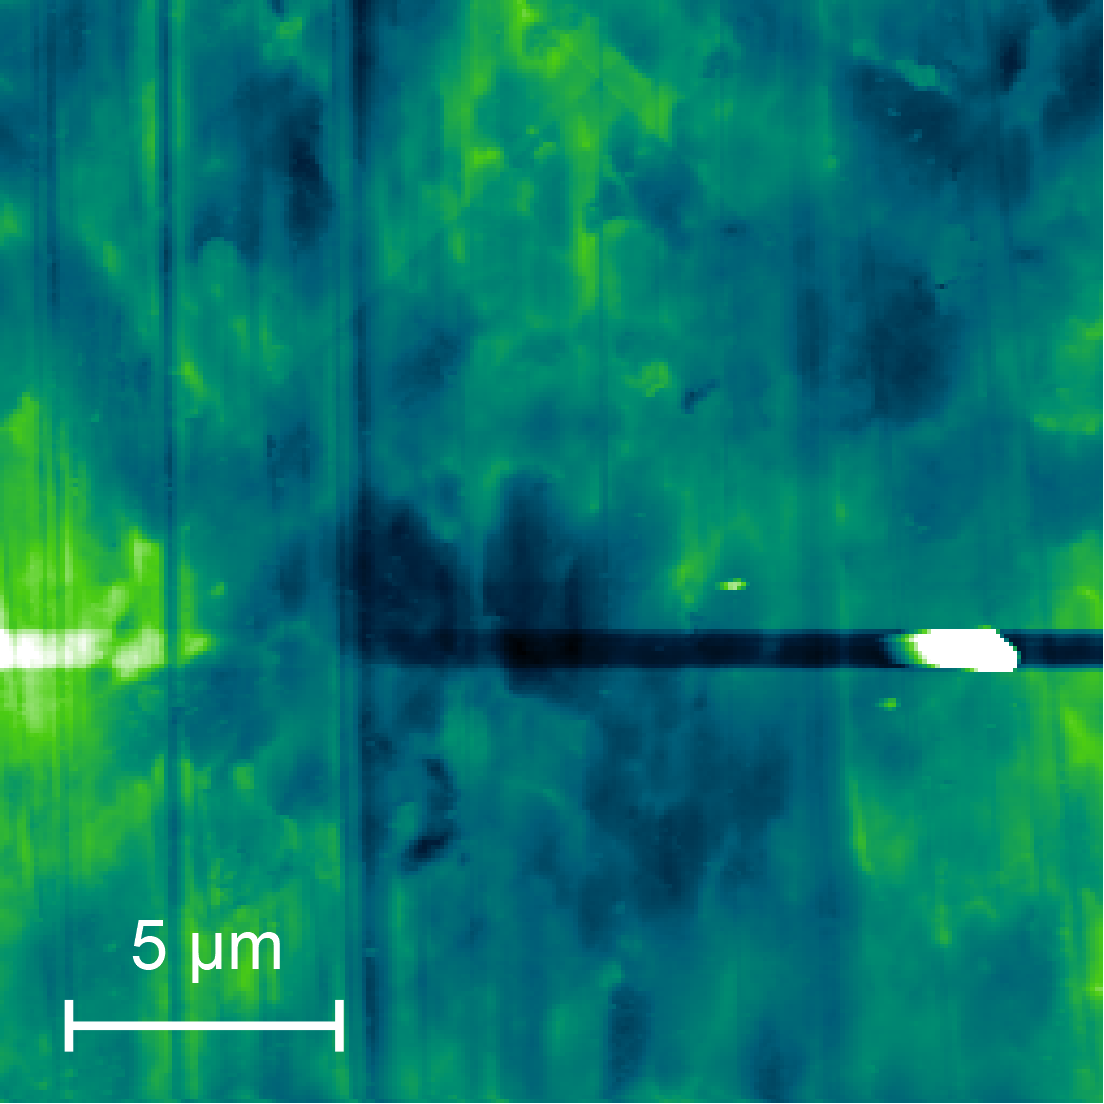
\includegraphics[width=0.25\textwidth]{./images/as_bought_zoomed_upper_half}
			\label{fig:foil-bought-afm}
		} \quad
		\subfigure[After etching.]{
			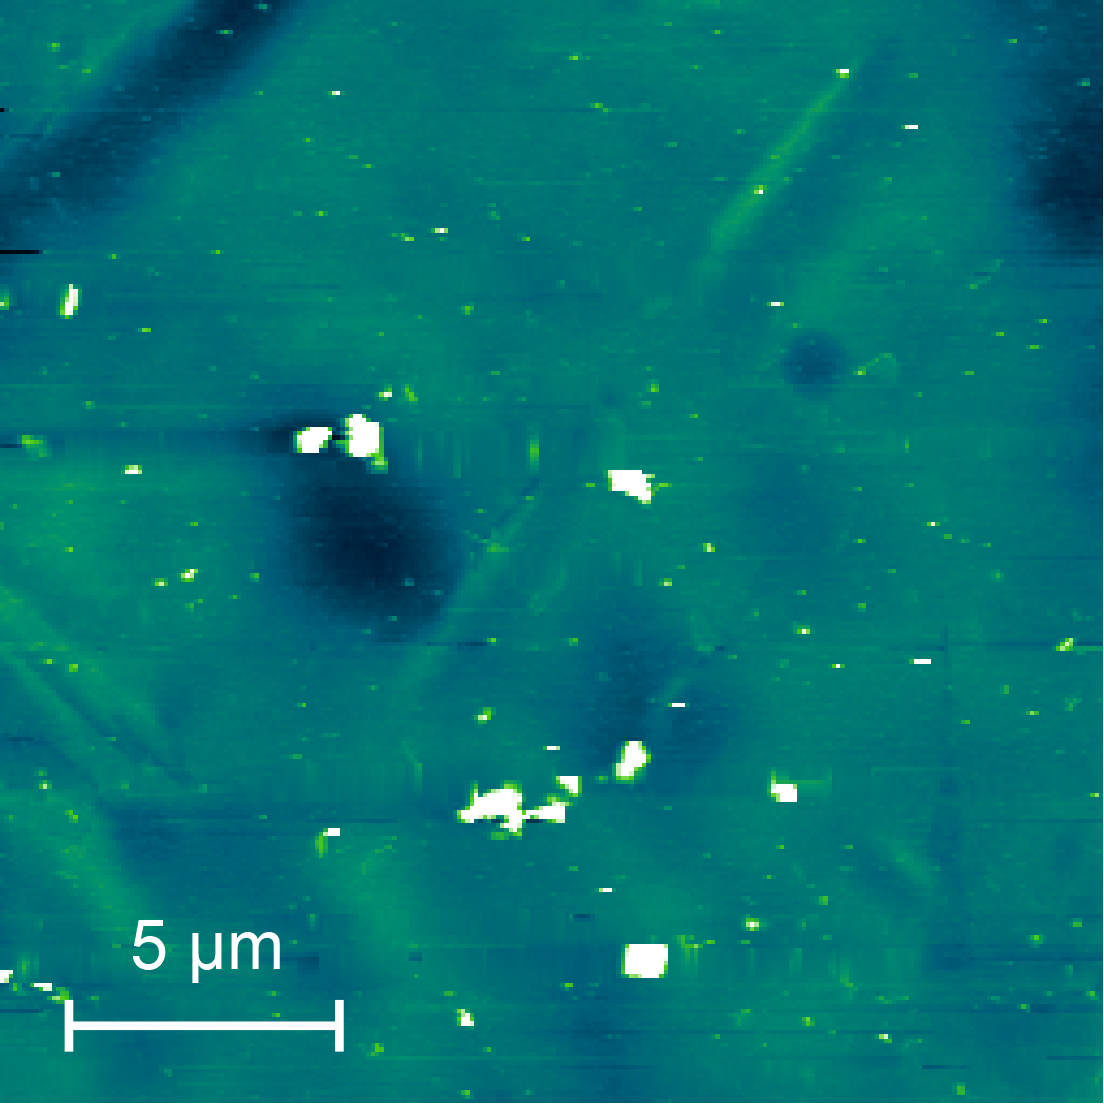
\includegraphics[width=0.25\textwidth]{./images/polished0000_zoomed_upper_half}
			\label{fig:foil-polished-afm}
		} 
		\subfigure[Height profiles before (red) and after (black) etching.]{
			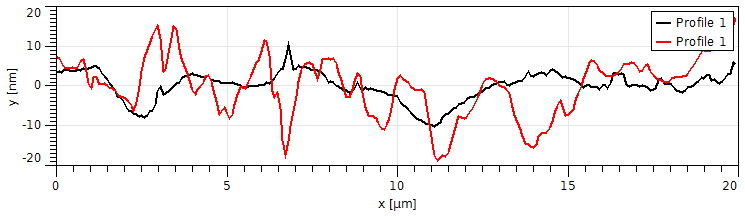
\includegraphics[width=0.4\textwidth]{./images/as_bought-polished_0000-profiles}
			\label{fig:foil-profiles}
		}
		\caption{RT-AFM topography image of copper foil as bought from Alfa Aesar \subref{fig:foil-bought-afm} before and \subref{fig:foil-polished-afm} after etching. \subref{fig:foil-profiles} Height profile averaged across the lower 10 lines of \subref{fig:foil-bought-afm} and \subref{fig:foil-polished-afm}. Roughness along the line profiles decreases after etching ($Rq_{before}=\SI{7.3}{\nano \meter} \rightarrow Rq_{after}=\SI{3.6}{\nano \meter}$). Color scale for both AFM images \SI{100}{\nano \meter}, Image width: \SI{20}{\micro \meter}}.
		\label{fig:foil-afm-as-bought}
	\end{figure}
	
	The surface of the copper foil is imaged with an uneven height distribution. As expected for a mechanically rolled foil, remnants of the production process can be seen. These striations run parallel from top to bottom and are typically narrower than \SI{1}{\micro \meter}. Their depth is in the range of \SIrange{10}{20}{\nano \meter} and thus comparable to the height variation present in between them. A line profile (\subref{fig:foil-profiles}, red) averages the lowest 10 lines of the image and helps to assess the surface height. Unwanted adsorbates are imaged as bright spots and are ignored in roughness analysis that is \SI{7.4}{\nano \meter}.
	
	%\begin{figure}[] \centering
	%	\subfigure[RMS $\approx$\SI{9}{\nm} in the left image, contrast \SI{100}{\nm}]{
	%	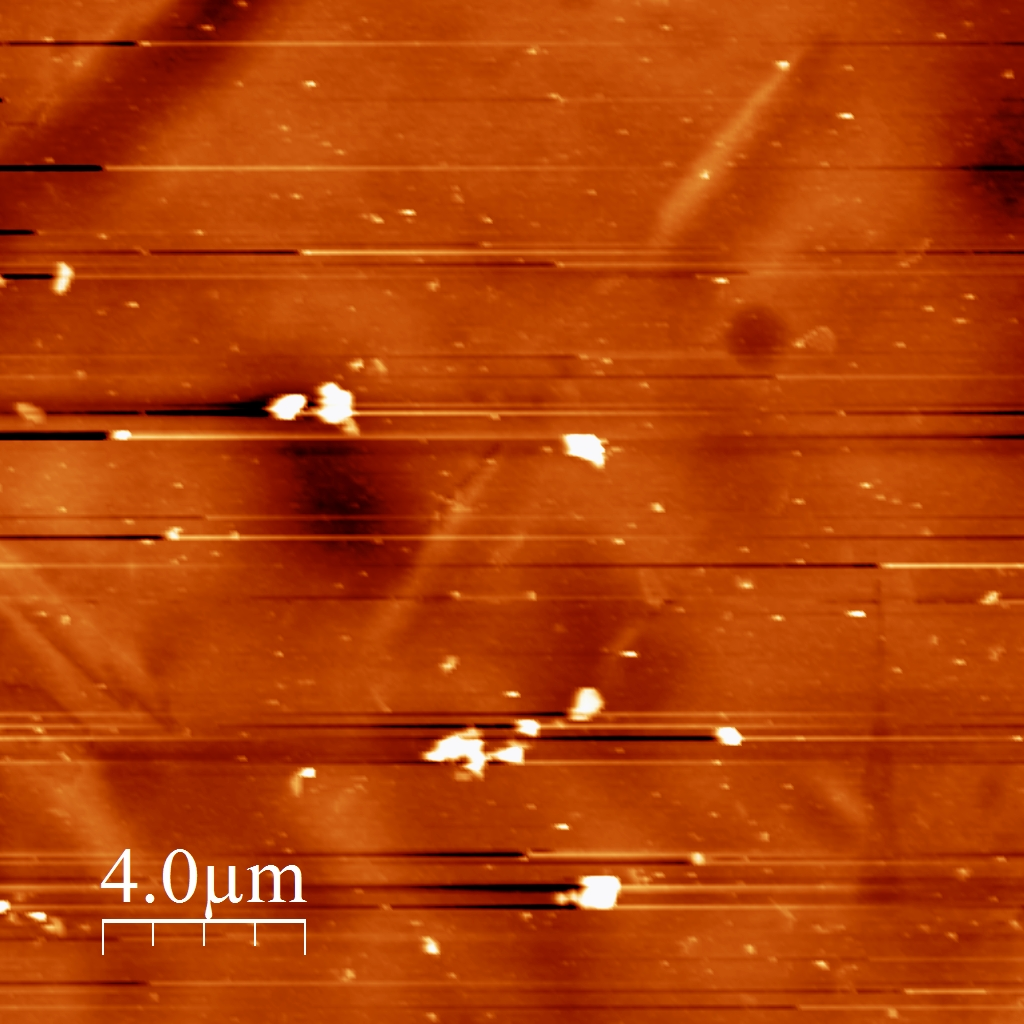
\includegraphics[width=0.4\textwidth]{./images/polished0000.jpg}
	%}
	%	\subfigure[RMS $\approx$\SI{3}{\nm} in the right image, contrast \SI{70}{\nm}]{
	%	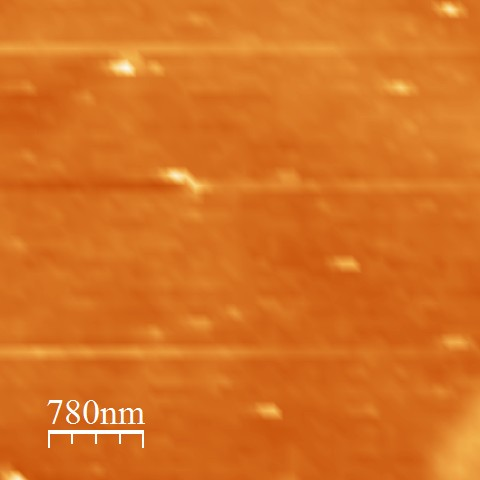
\includegraphics[width=0.4\textwidth]{./images/polished0001.jpg}
	%}
	%	\caption{AFM image of a copper foil polished 5h (according to table \ref{tab:used-etching-solution}), \textcolor{red}{\textbf{IMAGING PARAMETERS!}}}
	%	\label{fig:foil-afm-polished}
	%\end{figure}
	
	\autoref{fig:foil-afm-as-bought} show RT-AFM images in the same size and contrast - before \subref{fig:foil-bought-afm} and after \subref{fig:foil-polished-afm} etching.
	
	After etching (U=\SI{1.2}{\volt}, I=\SIrange{120}{250}{\mA} for \SI{5}{\hour} with solution shown in \autoref{tab:composition-etching-solution-I}) the striations vanish and the RMS value decreases by \SI{50}{\percent}. 
	The over all structure changes from a heterogeneous sample height to an even height distribution with far less ridges. Those present are less steep and sufficiently separated in space to exhibit flat regions in between where \textit{h}-BN may grow unperturbed. The circular depression is an result of bubbles affecting the rate of etching (compare \autoref{fig:SEM-2}).

%%%%%%%%%%%%%%%%%%%%%%%%%%%%%
\FloatBarrier
%%%%%%%%%%%%%%%%%%%%%%%%%%%%%

\newpage
\subsection{LT-STM characterization}
\label{section:foil-STM}
The bought and chemically polished foils are mounted on a sample holder and loaded into the load lock. It is evacuated for \SIrange{2}{3}{\hour}, afterwards the valve is opened to the chamber. During transfer, no notable increase in the base pressure is noted. The sample was initially degassed with slowly increasing temperatures to remove adsorbates like $CO, CO_2$ and $H_2O$. After some time of degassing, the sample was prepared with repeated sputter and anneal cycles. The annealing temperatures were increased up to \SI{800}{\degreeCelsius}. The sample was cooled down and observed in LT-STM.
		
Further experiments were carried out to increase the cleanliness of the \textit{h}-BN on the polycrystalline copper foil. To reduce the amount of elements coming from the body of the foil, it is repeatedly sputtered and annealed to temperatures as high as \SI{800}{\celsius}. This may have also a positive influence on the grain size and amount of corrugation. Several attempts have been made which are described in summary below.
%%%%%%%%%%%%%%%%%%%%%%%%%%%%%%%%%%%%%%%%%%%%%%%%%%%%%%%%%%%%%%%%%%%%%%%%%%%%%%%%%%%%%%%%%%
After cleaning, the sample is investigated in STM. The foil shows a in-homogeneous topography, with parts of the sample showing very flat regions while others still remain heavily corrugated and not scan able in STM.  A look onto the quite heterogeneous surface reveals flat areas with a typical roughness of $\approx \SI{70}{\pico\meter}$ exist (\autoref{fig:cu-foil-clean-stm-1}). Areas with very large corrugations $\geq \SI{100}{nm}$ exist and are hard to scan in STM and certainly bad places for \textit{h}-BN growth. Although being flat, the poly-crystalline foil shows a faceted surface with no long range order.
%%%%%%%%%%%%%%%%%%%%%%%%%%%%%%%%%%%%%%%%%%%%%%%%%%%%%%%

\begin{figure}[] \centering
	%	\subfigure[Roughness $\approx \SI{60}{\pico\meter}$.]{%
	%		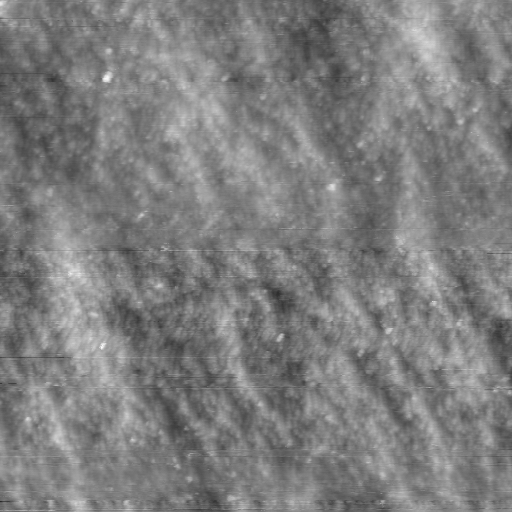
\includegraphics[width=0.45\textwidth]{./images/F150331-124839}
	%		\label{fig:30-31.03}
	%	}
	\subfigure[Cleaned copper foil before \textit{h}-BN growth. Surface shows many facets.
%	, the roughness is \SI{70}{\pico\meter}.
		]{%
		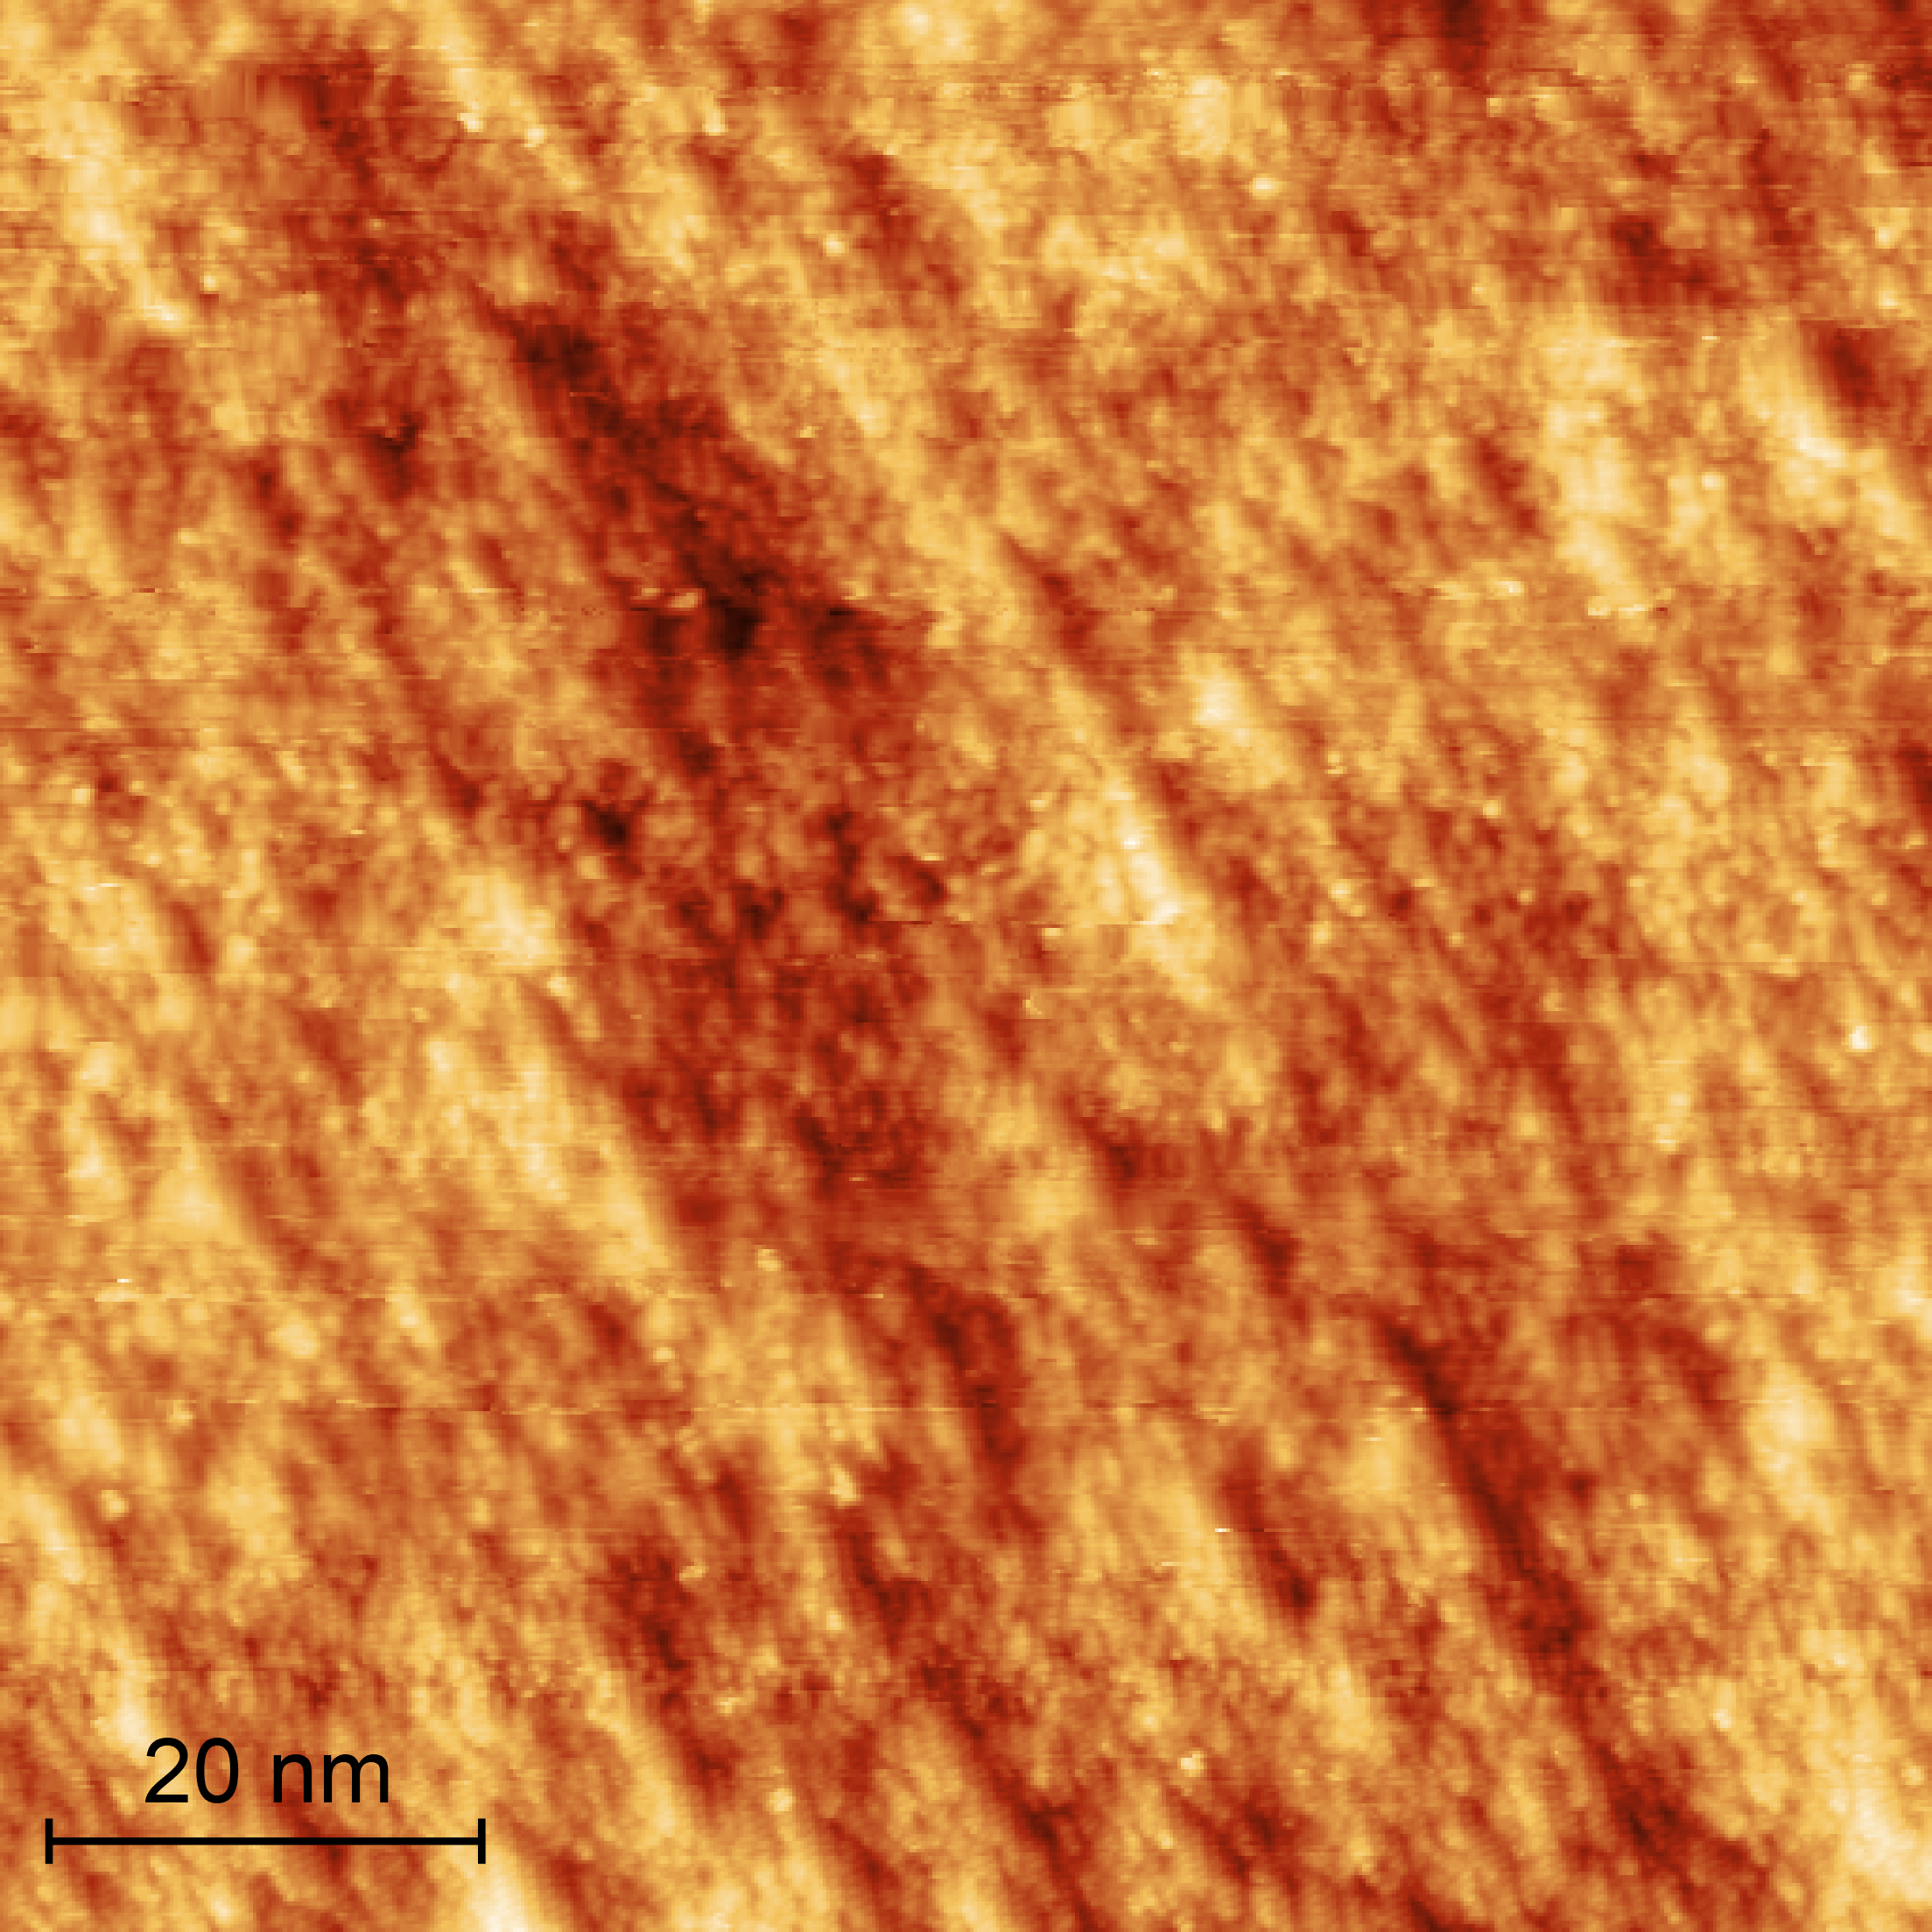
\includegraphics[width=0.4\textwidth]{./images/F150331-125720}
		\label{fig:cu-foil-clean-stm-1}
	} \quad
	%	\subfigure[STM image after \SI{4.5}{\langmuir} of borazine dosage on a \SI{750}{\celsius} hot copper foil surface. A small \textit{h}-BN island can be seen (lower right) on a largely uncovered copper foil background.]{%
	%		\includegraphics[width=0.45\textwidth]{./images/F150416-192611}
	%		\label{fig:F150416-192611}
	%	}
	%	\subfigure[STM image of \SI{22}{\langmuir} borazine dosed on a \SI{800}{\celsius} hot copper-foil surface. Several large islands can be seen that grow over Cu-foil step edges. Inset shows coverage with \textit{h}-BN ad layer in blue.]{
	%	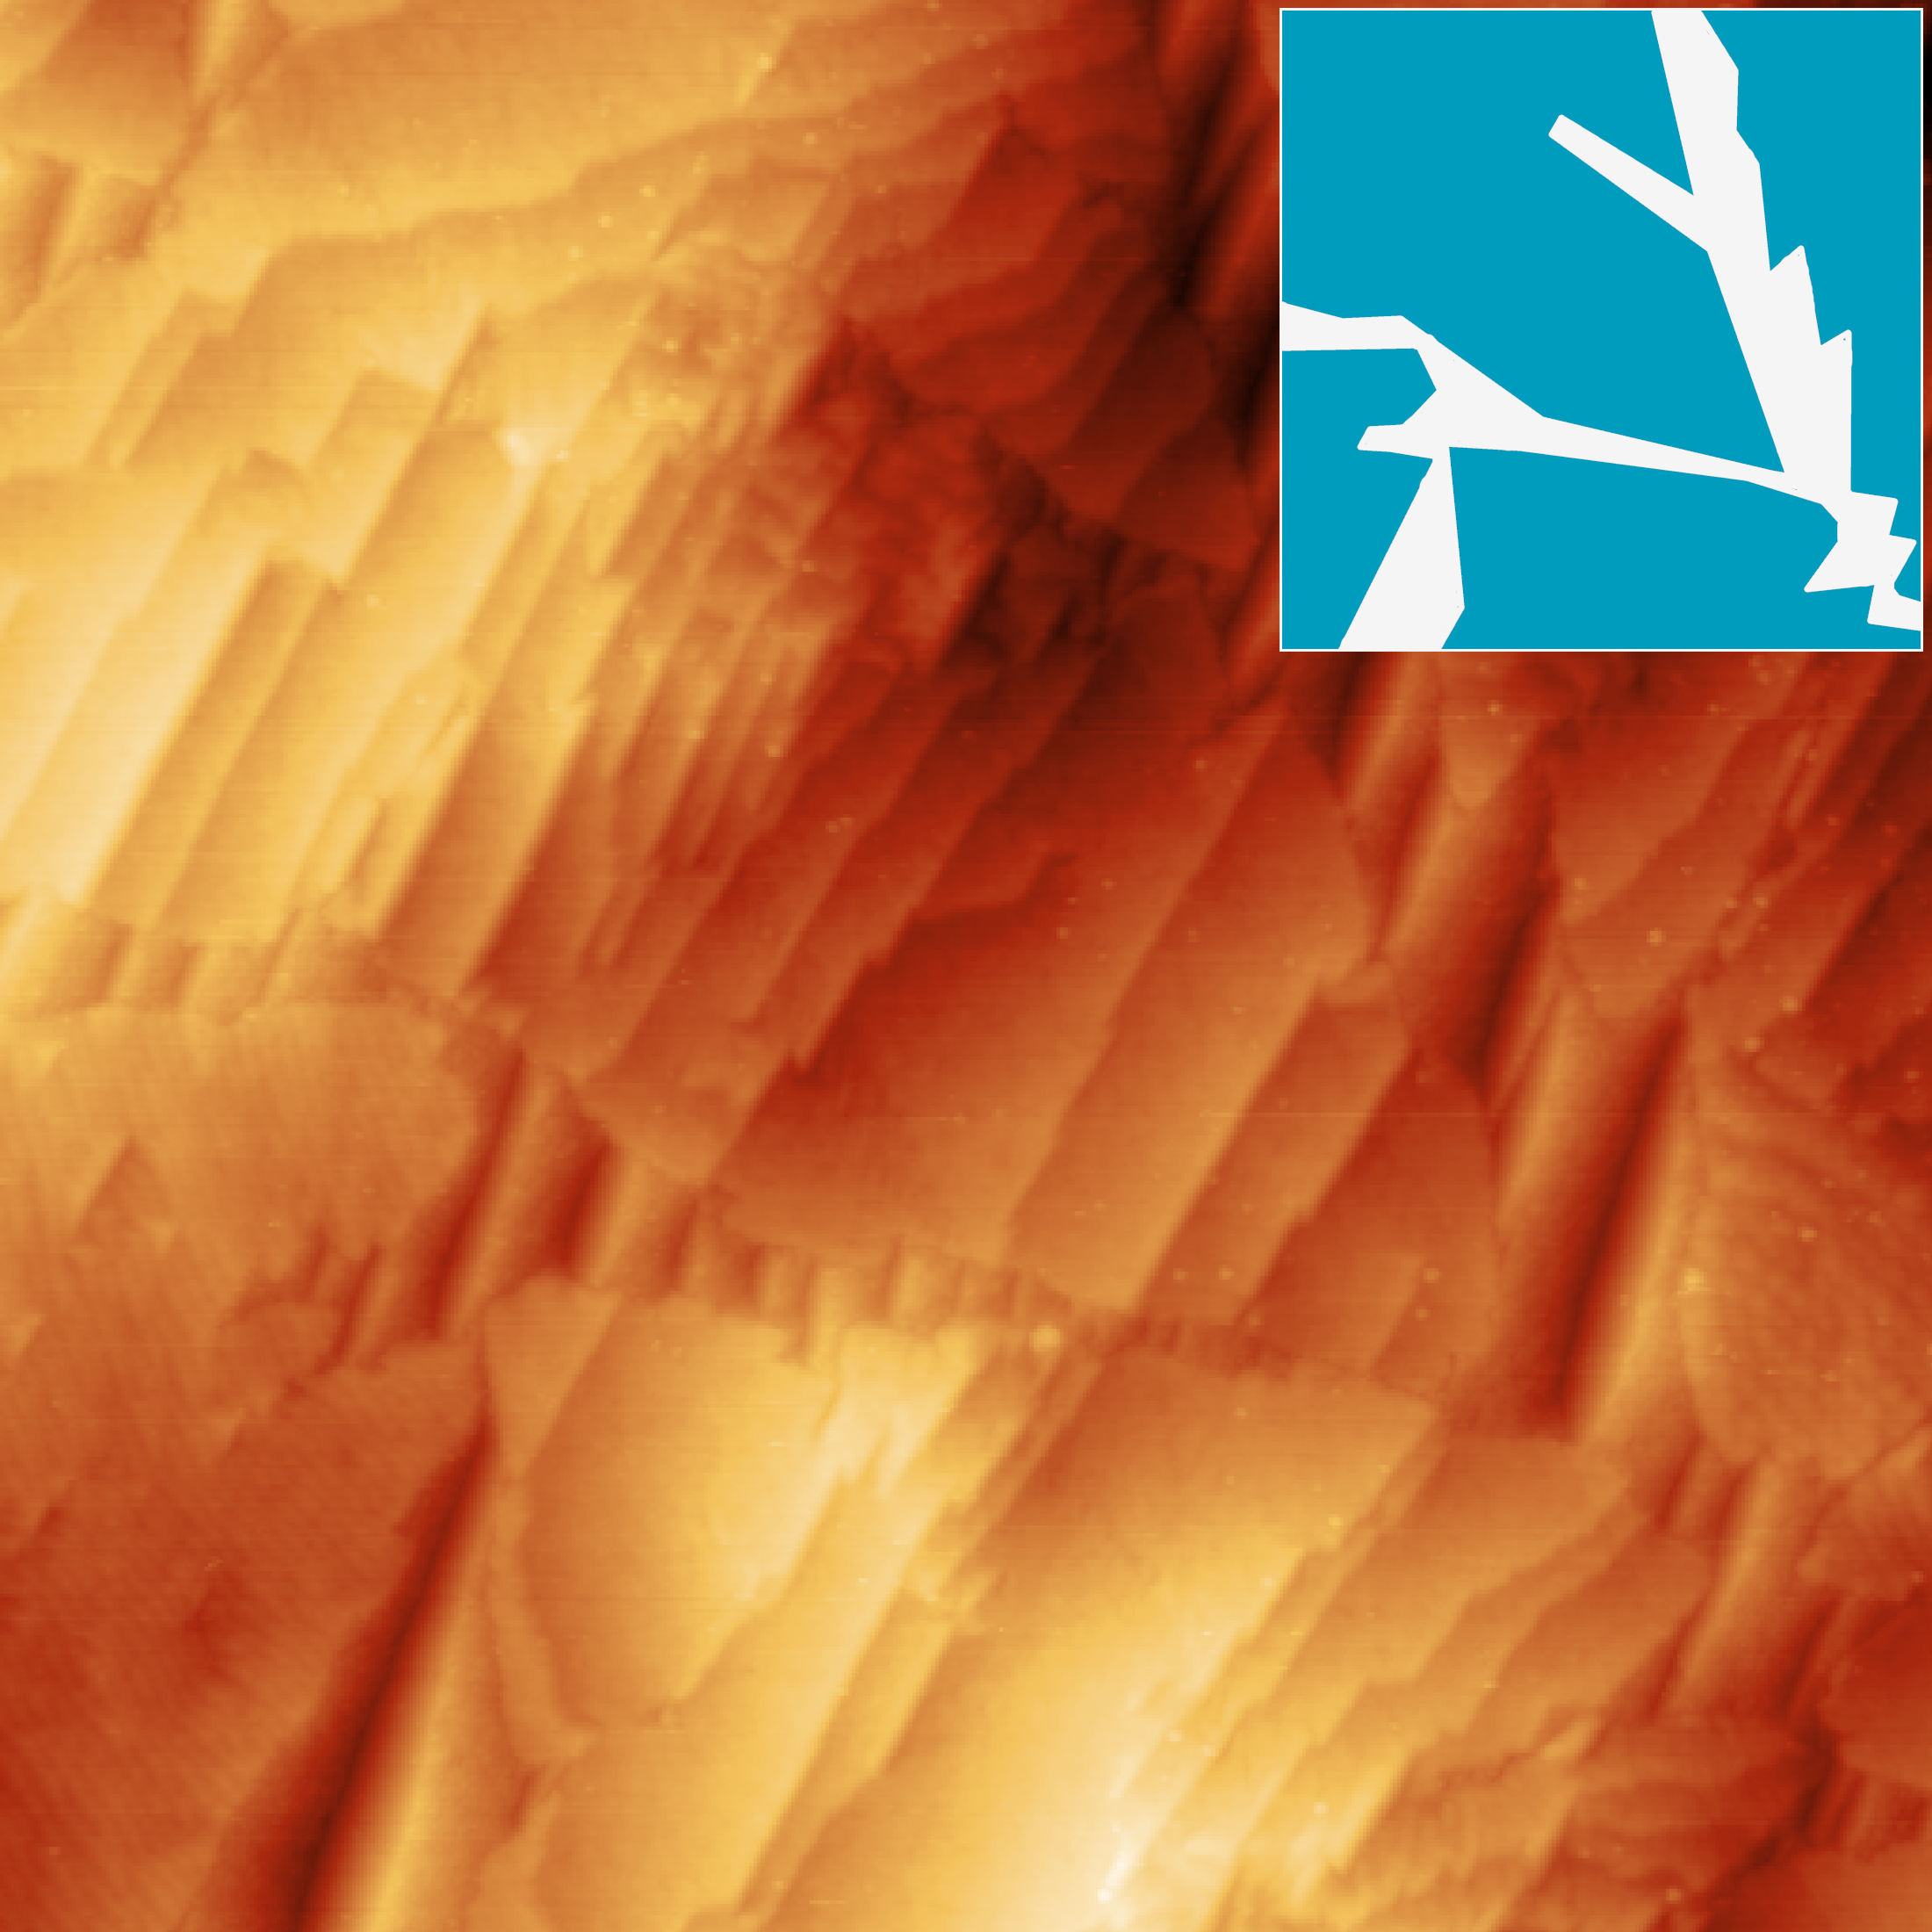
\includegraphics[width=0.35\textwidth]{./images/F150423-102732-with-inset}
	%	\label{cu-foil-hBN-stm}
	%}
	\subfigure[Typical height profile. The roughness is $R_q=\SI{70}{\pico\meter}$.]{%
		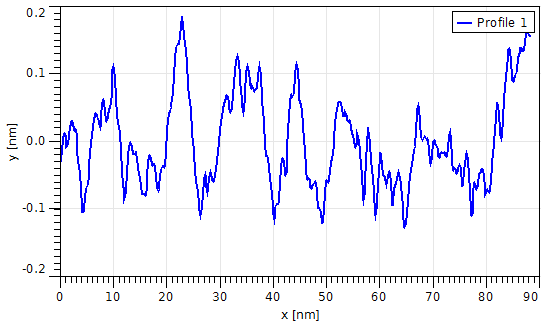
\includegraphics[width=0.4\textwidth]{./images/F150331-125720-profile}
		\label{fig:cu-foil-clean-profile}
	}
	\caption{Cu-foil \subref{fig:cu-foil-clean-stm-1} after repeated sputtering and annealing cycles. \subref{fig:cu-foil-clean-profile} Height profile. Imaging parameters: \subref{fig:cu-foil-clean-stm-1} \SI{3.6}{\volt}, \SI{0.1}{\nano\ampere}, color scale \SIrange{0}{600}{\pico\meter}, Image width: \SI{88,6}{\nano \meter}, 
		%	\subref{fig:F150416-192611} \SI{1}{\volt}, \SI{0.37}{\nano\ampere}, color scale \SIrange{0}{900}{\pico\meter}, Image width: \SI{44,3}{\nano \meter}.
		%\subref{{cu-foil-hBN-stm}} \SI{4.7}{\volt}, \SI{0.2}{\nano\ampere}, color scale \SIrange{0}{7}{\nano\meter}, Image width: \SI{295}{\nano \meter}
	}
\label{fig:cu-foil-clean-stm}
\end{figure}

%%%%%%%%%%%%%%%%%%%%%%%%%%%%%
\FloatBarrier
%%%%%%%%%%%%%%%%%%%%%%%%%%%%%

\subsection{SEM characterization} 
\label{sec:foil-SEM}
%	Invented in the 1930's by Manfred von Ardenne\cite{ardenne_elektronen-rastermikroskop_1938}, Scanning electron microscopy (SEM)\index{SEM} is another versatile tool for the experimentalist. In contrast to (LT-)STM and AFM, SEM is capable of imaging huge areas of the sample within a very short time, which allows for a vast overview as well as good statistics. Magnifications reach up to 500k and above, illustrating even features in the order of \SI{1}{\nano \meter}.

As the name already discloses, SEM scans the surface with electrons. Their interaction with the material are diverse and some of them are explained in the following. While all effects are present in every measurement, not every microscope features detectors for all of these. While detectors for secondary electrons are standard equipment others may be not.

%\begin{itemize}
% \item \textbf{Secondary electrons (SE)} are produced in the bulk by the high energetic primary electon beam within close proximity to the surface. This is why SEMs offer a very good resolution of the surface itself.
%  \item \textbf{Backscattered electrons (BSE)} are elastically scattered primary electrons. The resolution of this mode is not as high for the secondary electrons. The intensity of the BSE depends strongly on the the atomic number Z of the specimen. It is useful for a complementary view, for example when chemical composition is of high interest.
%  Electron backscatter diffraction (EBSD) is used to achieve information on the crystallographic structure of a specimen.
% \item \textbf{Characteristic X-Rays} are used to identify the composition and measure the abundance of elements in the sample, too. See section \ref{sec:XPS} and figure \ref{fig:auger-core} therein for more details.
% \item \textbf{Cathodoluminescence (CL)} happens when electrons hit a material and exite photons. This effect is used in televesion screens where high energetic electrons are accelerated onto a screen containing phosphorus. There they distribute their energy with many others, some of those loose energy in form of photons which wavelenghts are within the visible spectrum. These light is called cathodoluminescence.
% \end{itemize}

The primary electrons are created with a filament. These often consist of tungsten (metal, high melting point, low work function). Alternatives are lanthanum hexaboride ($\textnormal{LB}_6$) - often used in LEED setups, too - or zirconium oxide.
Electrons are accelerated (typical energies are within \SIrange{1}{40}{\kilo \eV}) and focused on the specimen surface in a spot with few \si{nm} diameter with condenser lenses. Scanning the surface is achieved with coils that deflect the electron beam and therefore the actual scanning spot.

When the electrons hit the surface, they interact with the specimen in a small volume. The volume depends on the electron's energy, the atomic number Z of the specimen and the specimen's density. It is typically in the order of \SIrange{0.1}{5}{\micro \meter}.

Drawbacks:
\begin{itemize}
 \item[-] Sample has to be mounted $\rightarrow$ no in-situ measurement, surface alteration in between
 \item[-] Rather ``dirty'' vacuum $\rightarrow$ surface alteration while measuring
 \item[-] Measurement destroys sample $\rightarrow$ adsorbate build-up due to chemical reaction below e-beam
\end{itemize}



\begin{figure}\centering
	\subfigure[\SI{570}{\micro \meter}$\times$\SI{380}{\micro \meter}]{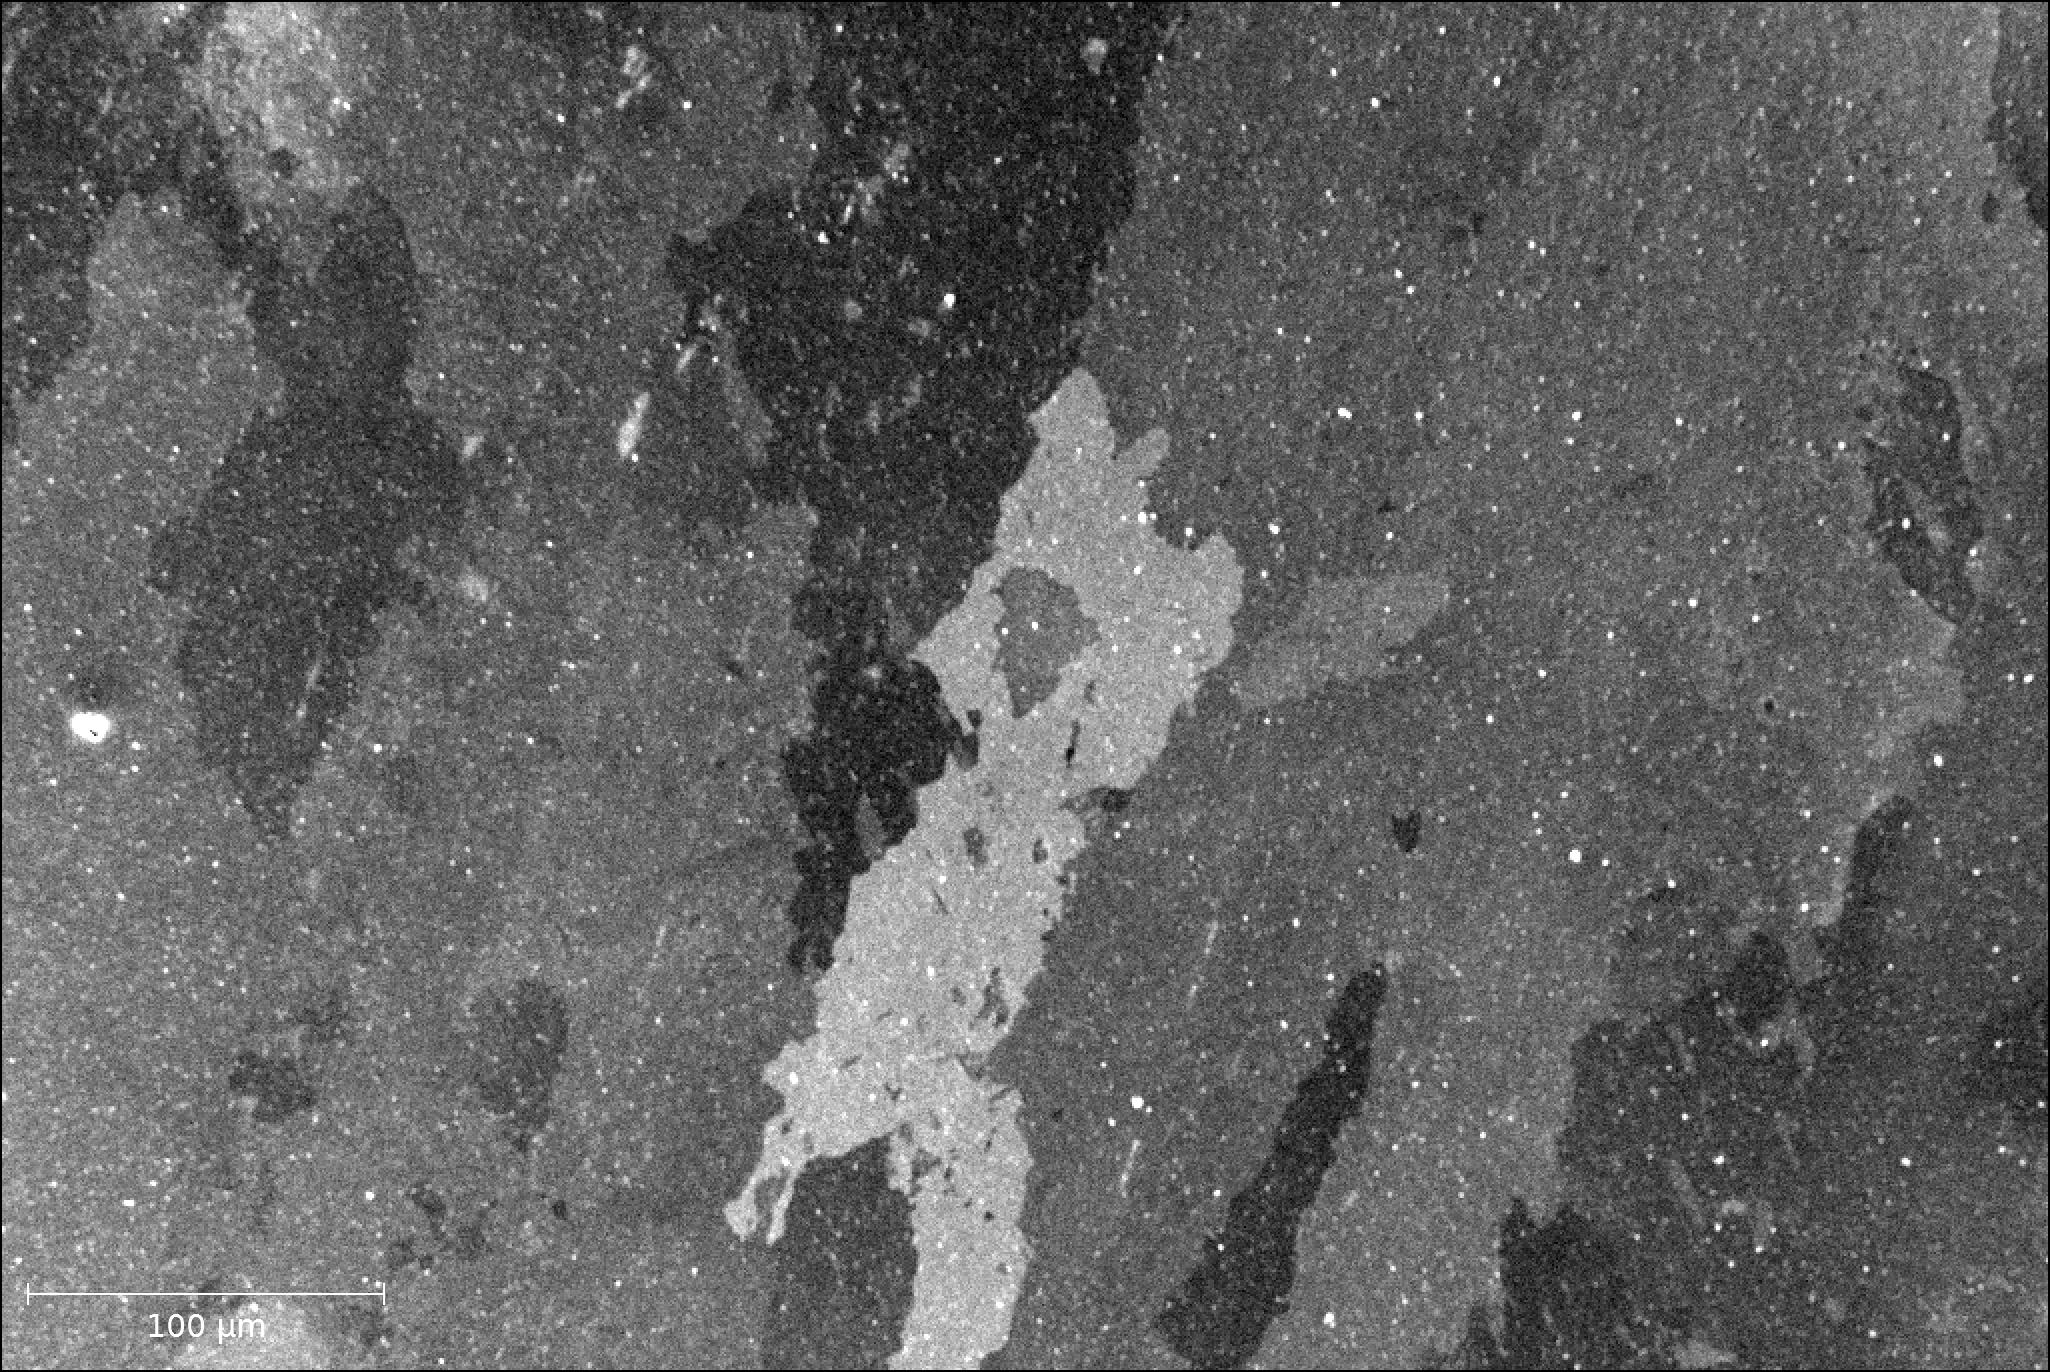
\includegraphics[width=0.7\textwidth]{./images/Domenik_16031715}
		\label{fig:SEM-1}
	}
	\subfigure[\SI{18}{\micro \meter}$\times$\SI{12}{\micro \meter}]{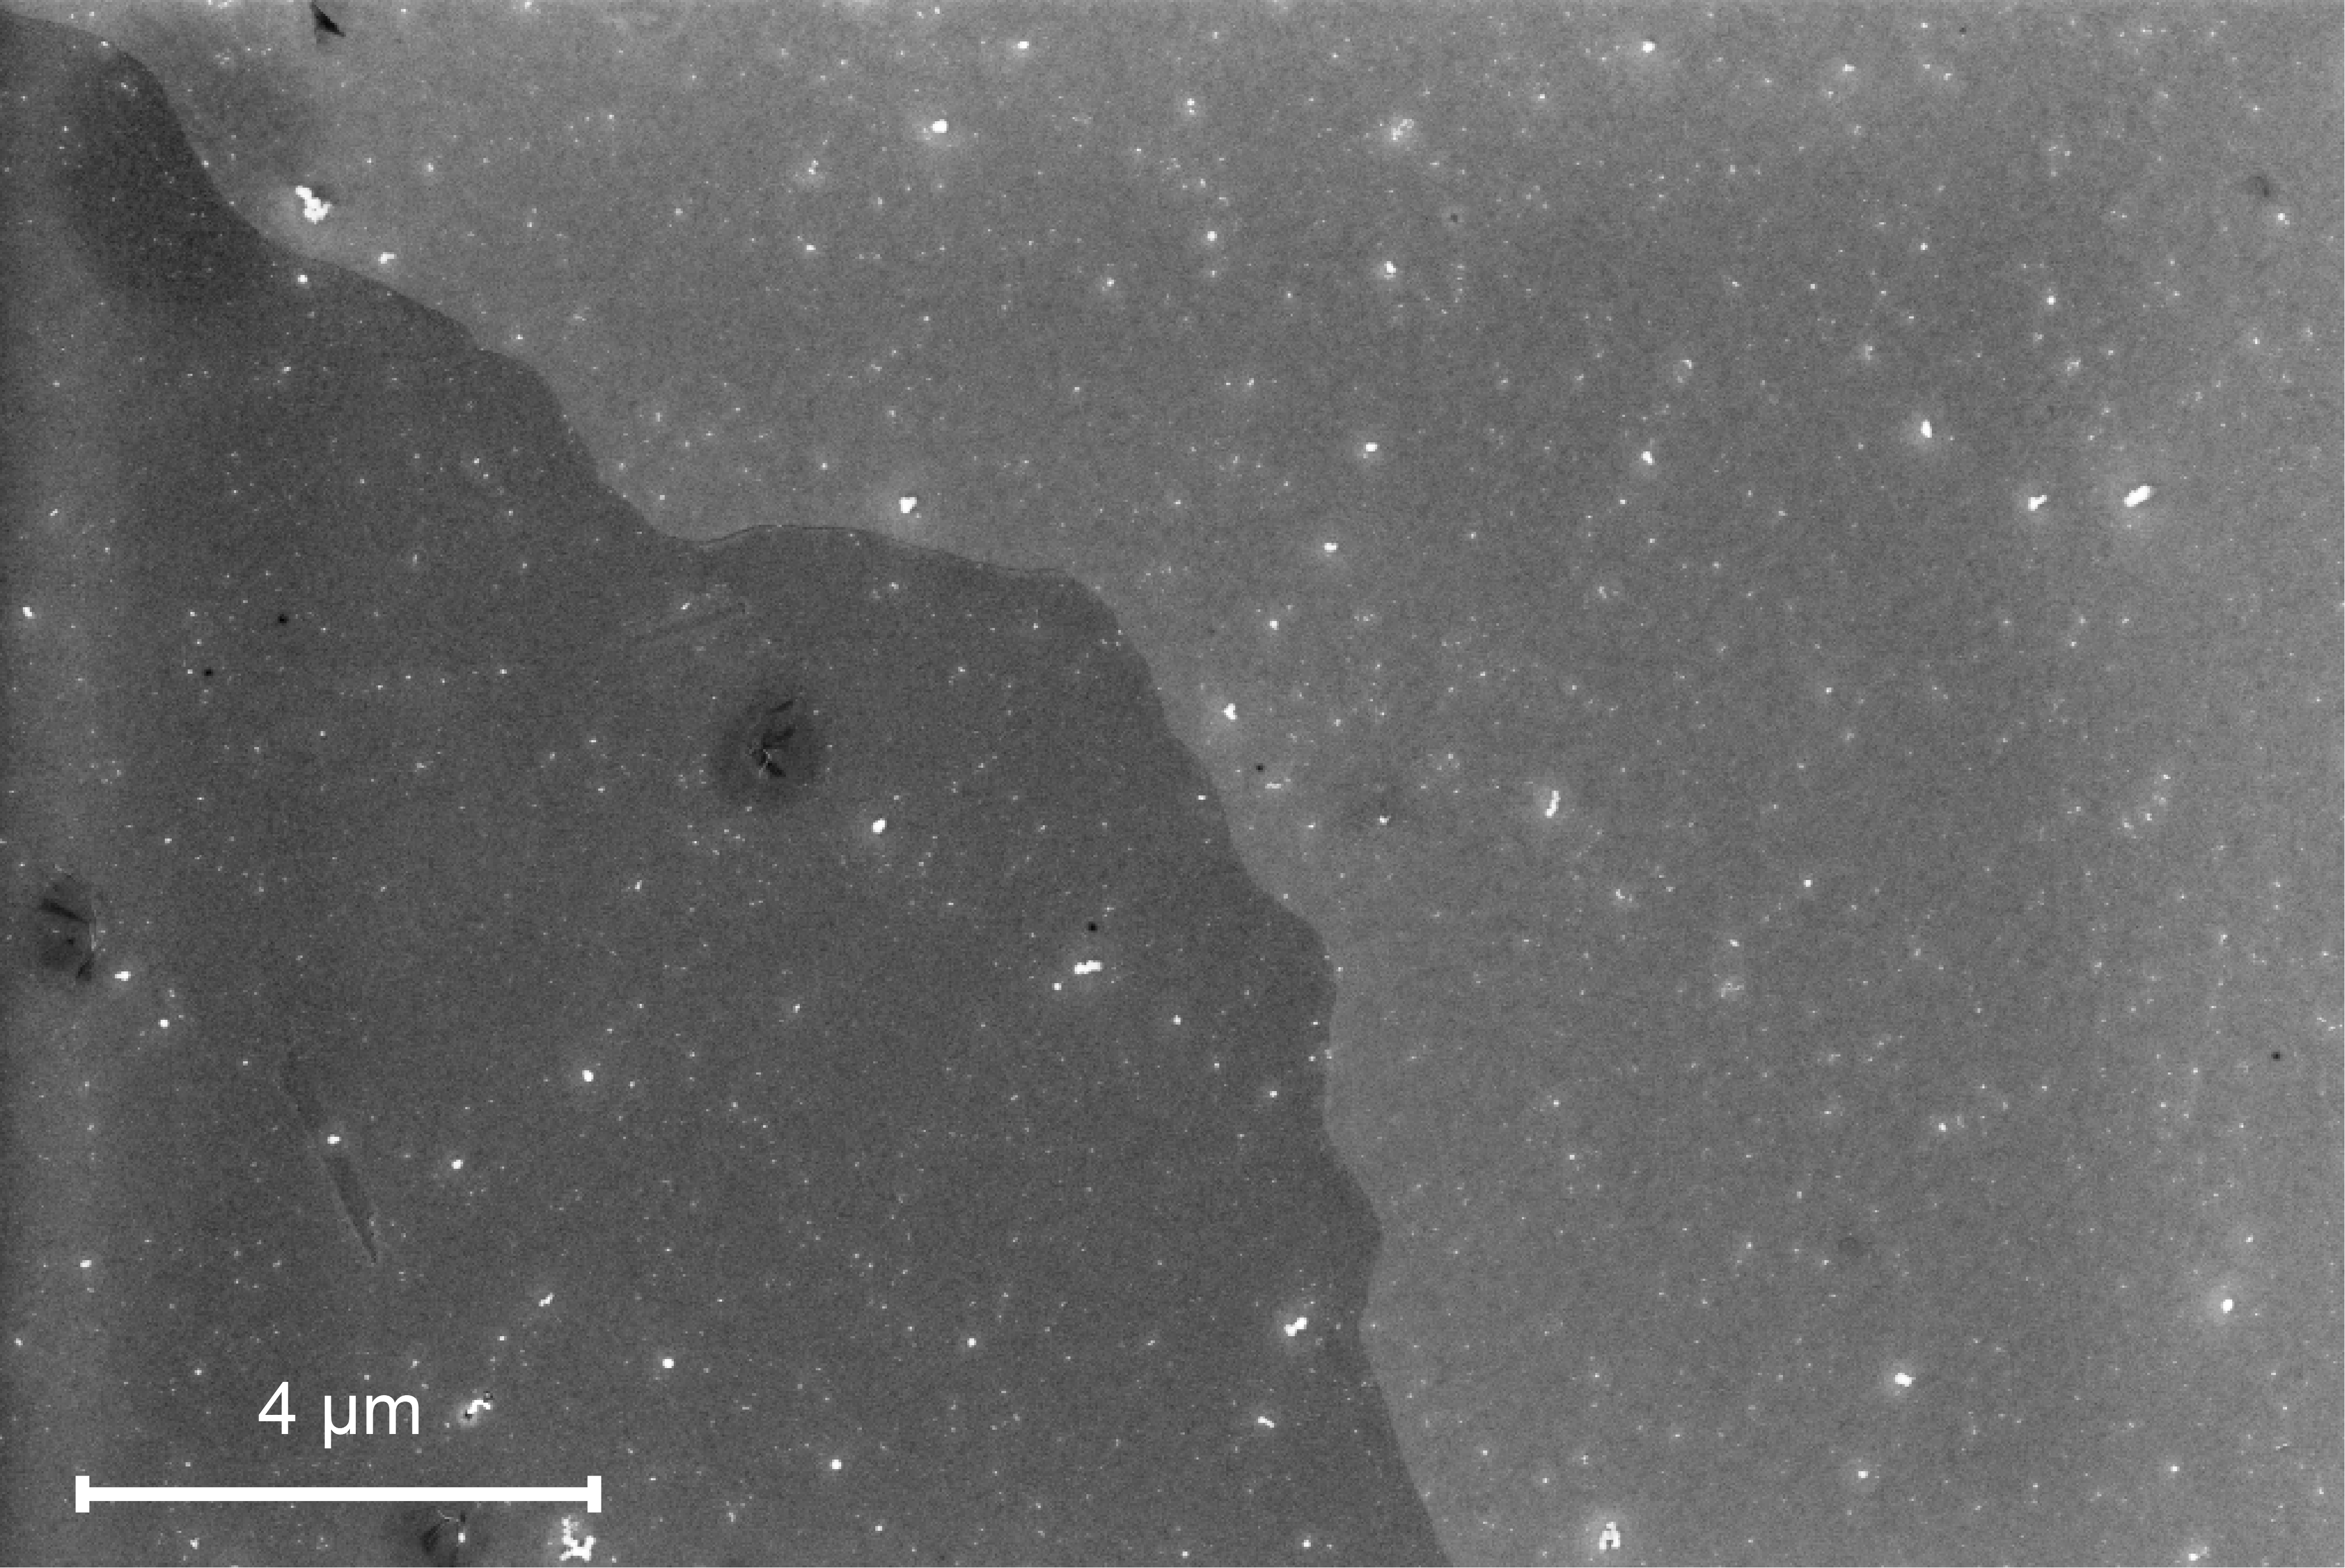
\includegraphics[width=0.33\textwidth]{./images/Domenik_16031717}
		\label{fig:SEM-2}
	} \quad
	\subfigure[\SI{5.6}{\micro \meter}$\times$\SI{3.7}{\micro \meter}]{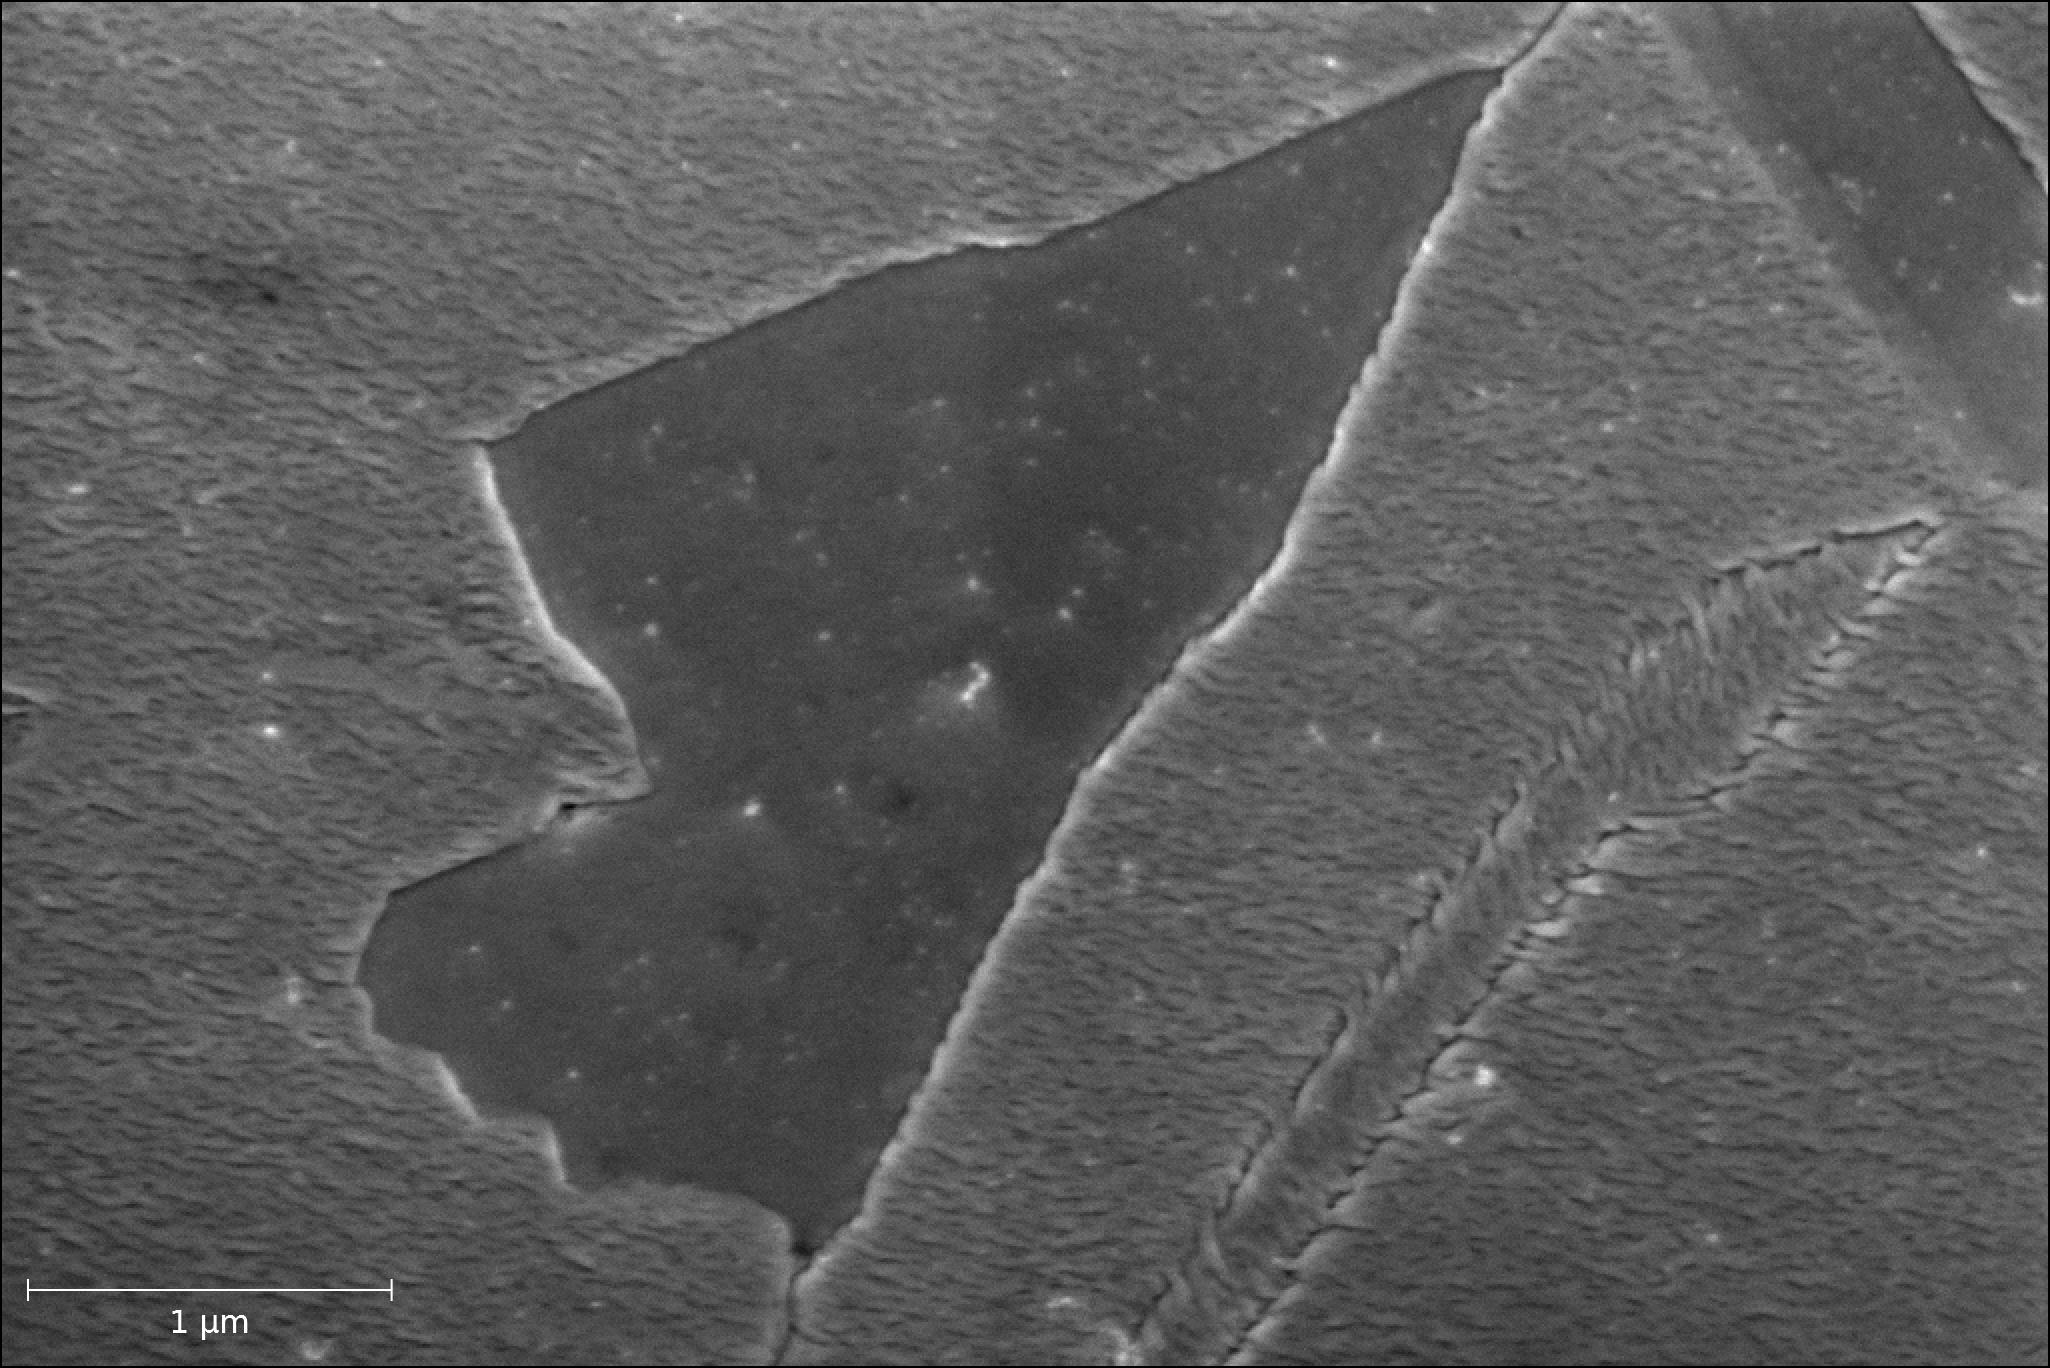
\includegraphics[width=0.33\textwidth]{./images/Domenik_16031700}
		\label{fig:SEM-3}
	}
	\caption{SEM image of etched copper foil. Different contrast suggests different grain-orientation within the surface. \subref{fig:SEM-1} Larger image showing the contrast of different grains in the copper-foil, \subref{fig:SEM-2} zoom to an area with two different contrasts and their border. \subref{fig:SEM-3} A dark grain is embedded in an otherwise curly surface. On both, bright small features are visible and attributed to an inhomogeneous etching process. Recorded with U=\SI{5}{\kilo \eV}.}
	\label{fig:SEM-gb}
\end{figure}

One of the foils is blown dry with nitrogen to remove isopropyl alcohol remnants and is put into the loading stage of a \textbf{s}canning \textbf{e}lectron \textbf{m}icroscope (SEM). After operating conditions are met, a series of images is recorded to characterize the overall surface structure of the foil. 

\autoref{fig:SEM-1} shows a typical surface area. It is apparent that it is imaged in different intensities. According to \cite{wu_effects_2015, wendt_correlation_2007, langlois_crystal_2015} these are attributed to the copper grain orientation within the foil due to their differing resistivity. The derived grain size ranges from a few \SI{}{\micro \meter} to several hundred \SI{}{\micro \meter}. Many grains show distinct intensity differences compared to their neighbors, e.g. in the center region are several easily distinguishable grains. But there are regions where a similar grain intensity makes it hard to attribute different grains to a surface area.

A border region is shown in \autoref{fig:SEM-2} with larger magnification. Two grains are separated by a boundary running from top left to bottom center. It is irregularly shaped and does not show a preferred direction of propagation.

Three darker circles in the top left image indicate the presence of different etching rates. Their origin is attributed to the presence of gaseous bubbles that hinder the etchant to immerse the copper surface at all times. The different surface treatment results in a change in contrast in SEM. These features are not frequent enough to co-determine the surface structure.

Smaller bright spots are spread across the image area. Here the conductivity of the specimen is larger so that more electrons are accounted for in the detector. Their size is much smaller and they appear on every image. No long range order can be found but they show similarities to features present for crystal defects after etching. 

The copper foil shows different surface morphologies. While some areas appear as wavy structure in SEM, others are much flatter. \autoref{fig:SEM-3} displays a grain that appears darker than its surrounding and incorporates some bright small spots. The outline shows no obvious corner geometry so that the overall shape of the grain appears asymmetric. 

Although the contrast between neighboring grains is clearly visible for this first example, a second smaller, elongated grain is embedded in the lower right part of the image. Its contrast resembles the surrounding, but a border is visible as dark, fuzzy lines. In contrast to the first example, the inside of this grain merges with its surrounding via many small connections. These bridges across the boundary hinder the grain distinction from the embedding grain. 

Although the contrast and morphology is very similar, one can see a change in the copper grain surface as it changes its orientation. One can see this as change in propagation direction of the wavy surface. While for the large grain the waves run from top to bottom, the inset grain appears to change their propagation direction to be more horizontal.

No direct determination of the grains' facet orientation has been done due to the lack of EBSD-data in the used SEM setup.

%	\begin{figure}[] \centering
%		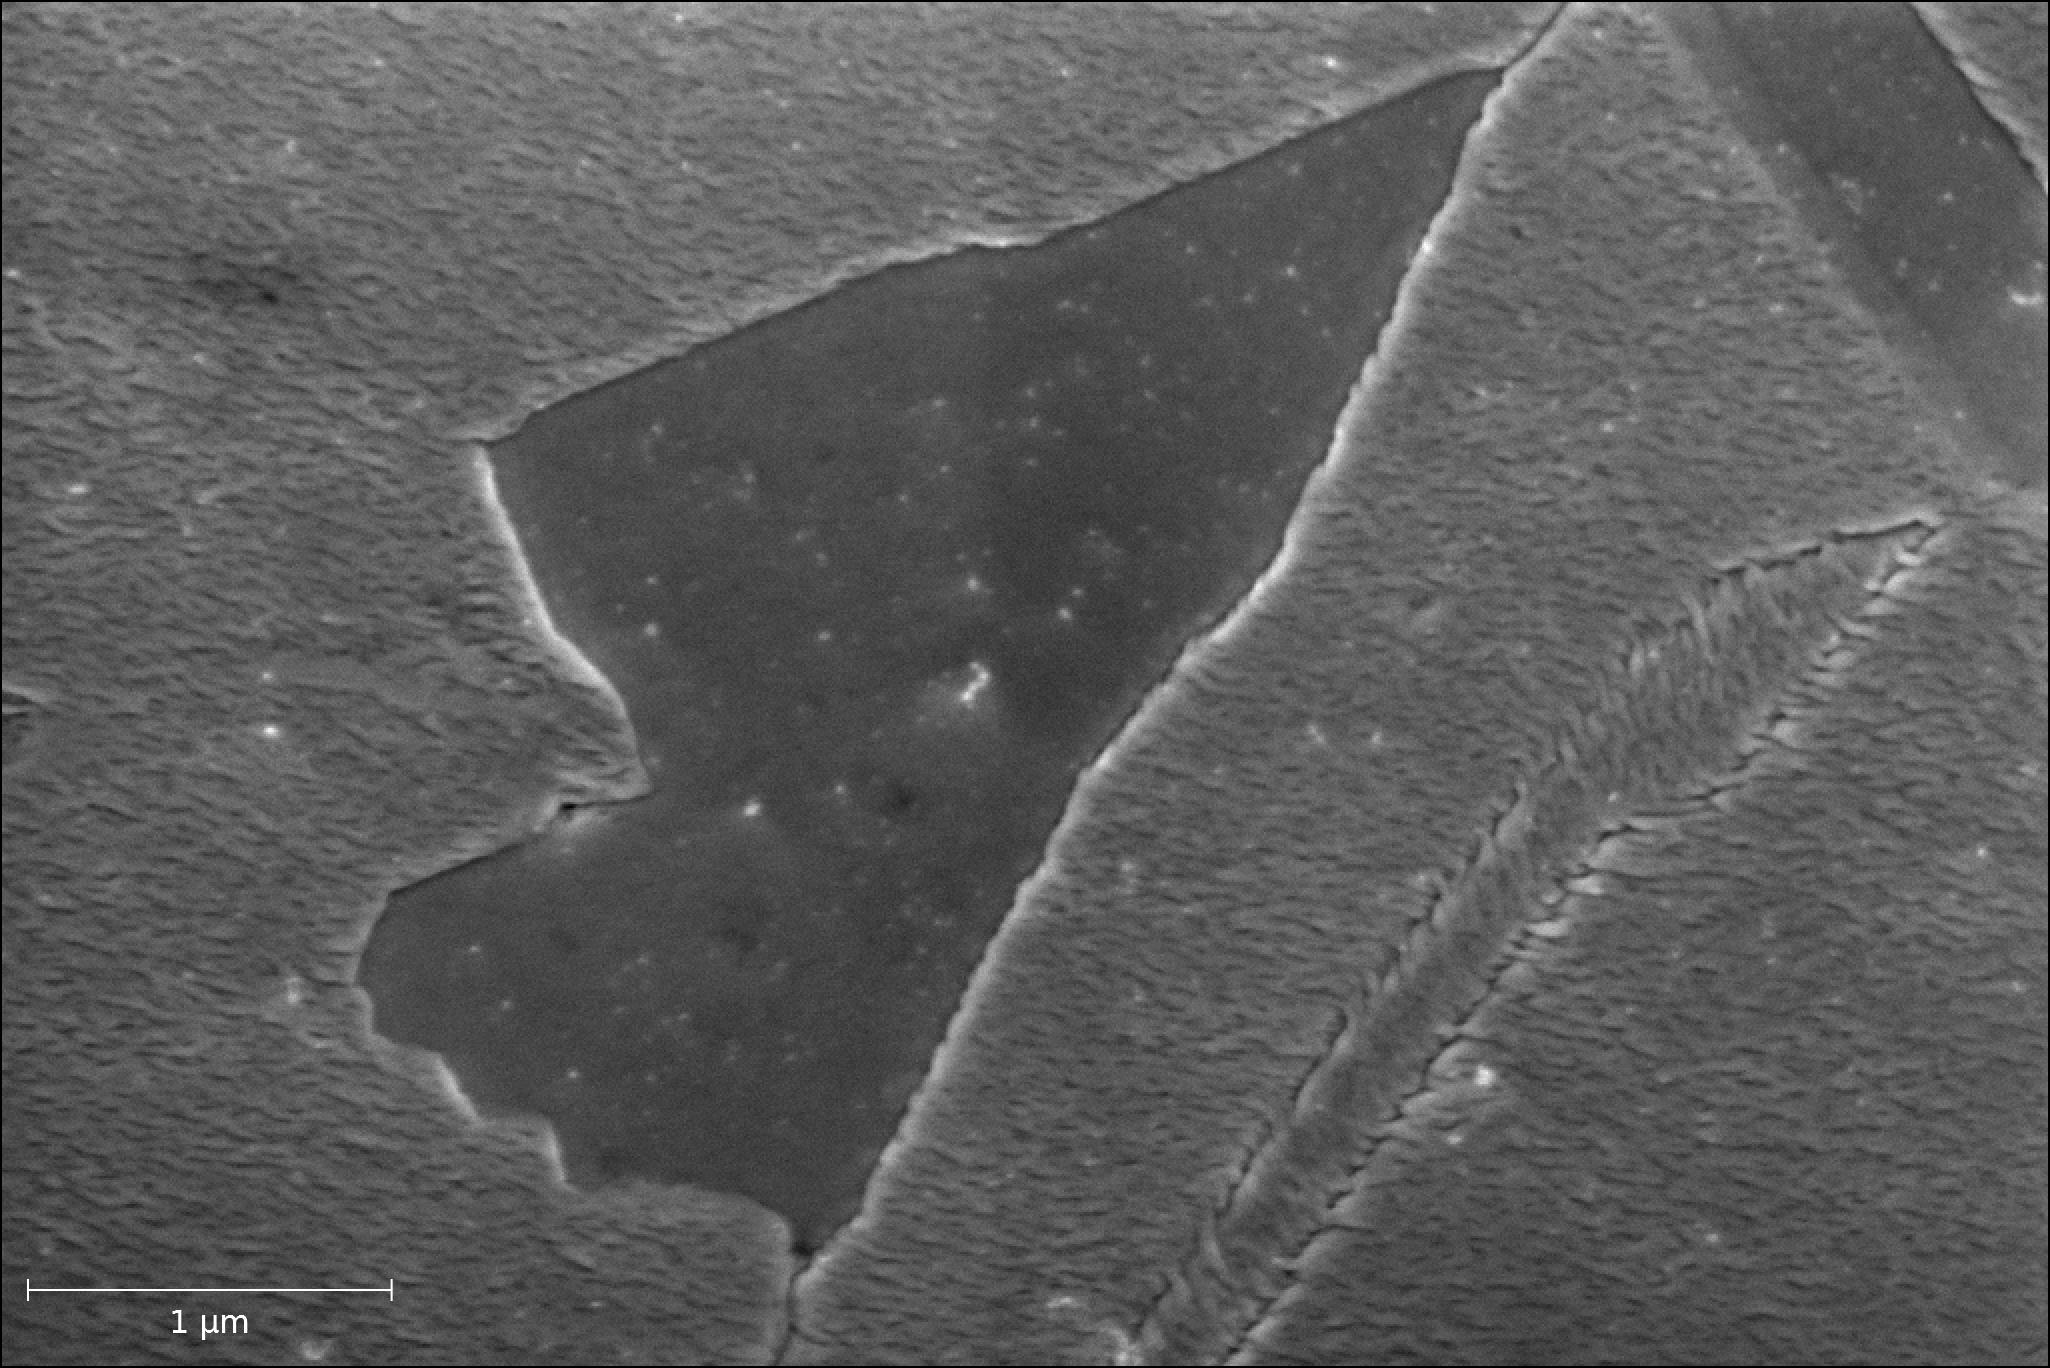
\includegraphics[width=0.7\textwidth]{./images/Domenik_16031700.jpg}
%		%\includegraphics[height=6cm]{../Daten/SEM/160317-Domenik/Domenik_16031717.jpg}
%		\caption{Close up SEM image that shows different surface morphologies after polishing (\SI{5.6}{\micro \meter}$\times$\SI{3.7}{\micro \meter}). A dark grain is embedded in an otherwise curly surface. On both, bright small features are visible and attributed to an inhomogeneous etching process. Recorded with U=\SI{5}{\kilo \eV}}
%		\label{fig:SEM-surface}
%	\end{figure}

%%%%%%%%%%%%%%%%%%%%%%%%%%%%%
\FloatBarrier
%%%%%%%%%%%%%%%%%%%%%%%%%%%%%
\newpage

\section{CVD-Growth of \textit{h}-BN with borazine}
The sample was sputtered and annealed several times to temperatures of \SI{800}{\celsius}. Before the dosage it was held 5 minutes at \SI{750}{\celsius}. Borazine was dosed with the same pressure as before (\SI{1e-7}{\milli \bar}) but for \SI{1}{\minute} and at a lower temperature of \SI{750}{\celsius}. After the preparation the sample was kept at \SI{750}{\celsius} for another minute. It was cooled down slowly.
	 \subsection{LT-STM characterization}
%The foil was sputtered and annealed 4 times with temperatures of \SI{800}{\celsius}. Borazine was dosed at \SI{2e-7}{\milli \bar} for \SI{2.5}{\minute}. The sample was kept at \SI{750}{\celsius} for another 5 minutes after dosing. The sample was cooled down slowly. \autoref{fig:h-bn-overgrown-cu-1} shows some of the grown islands. The copper surface changes upon \textit{h}-BN growth and the terrace width increases below the \textit{h}-BN flakes. The typical faceting of the surface vanishes or can at least not be depicted because of the overgrowing \textit{h}-BN (\autoref{fig:h-bn-overgrown-cu-2}). 

	% -----------BILDER ---- DISKUSSION: 21.04
	%\begin{figure}
	% \centering
	% 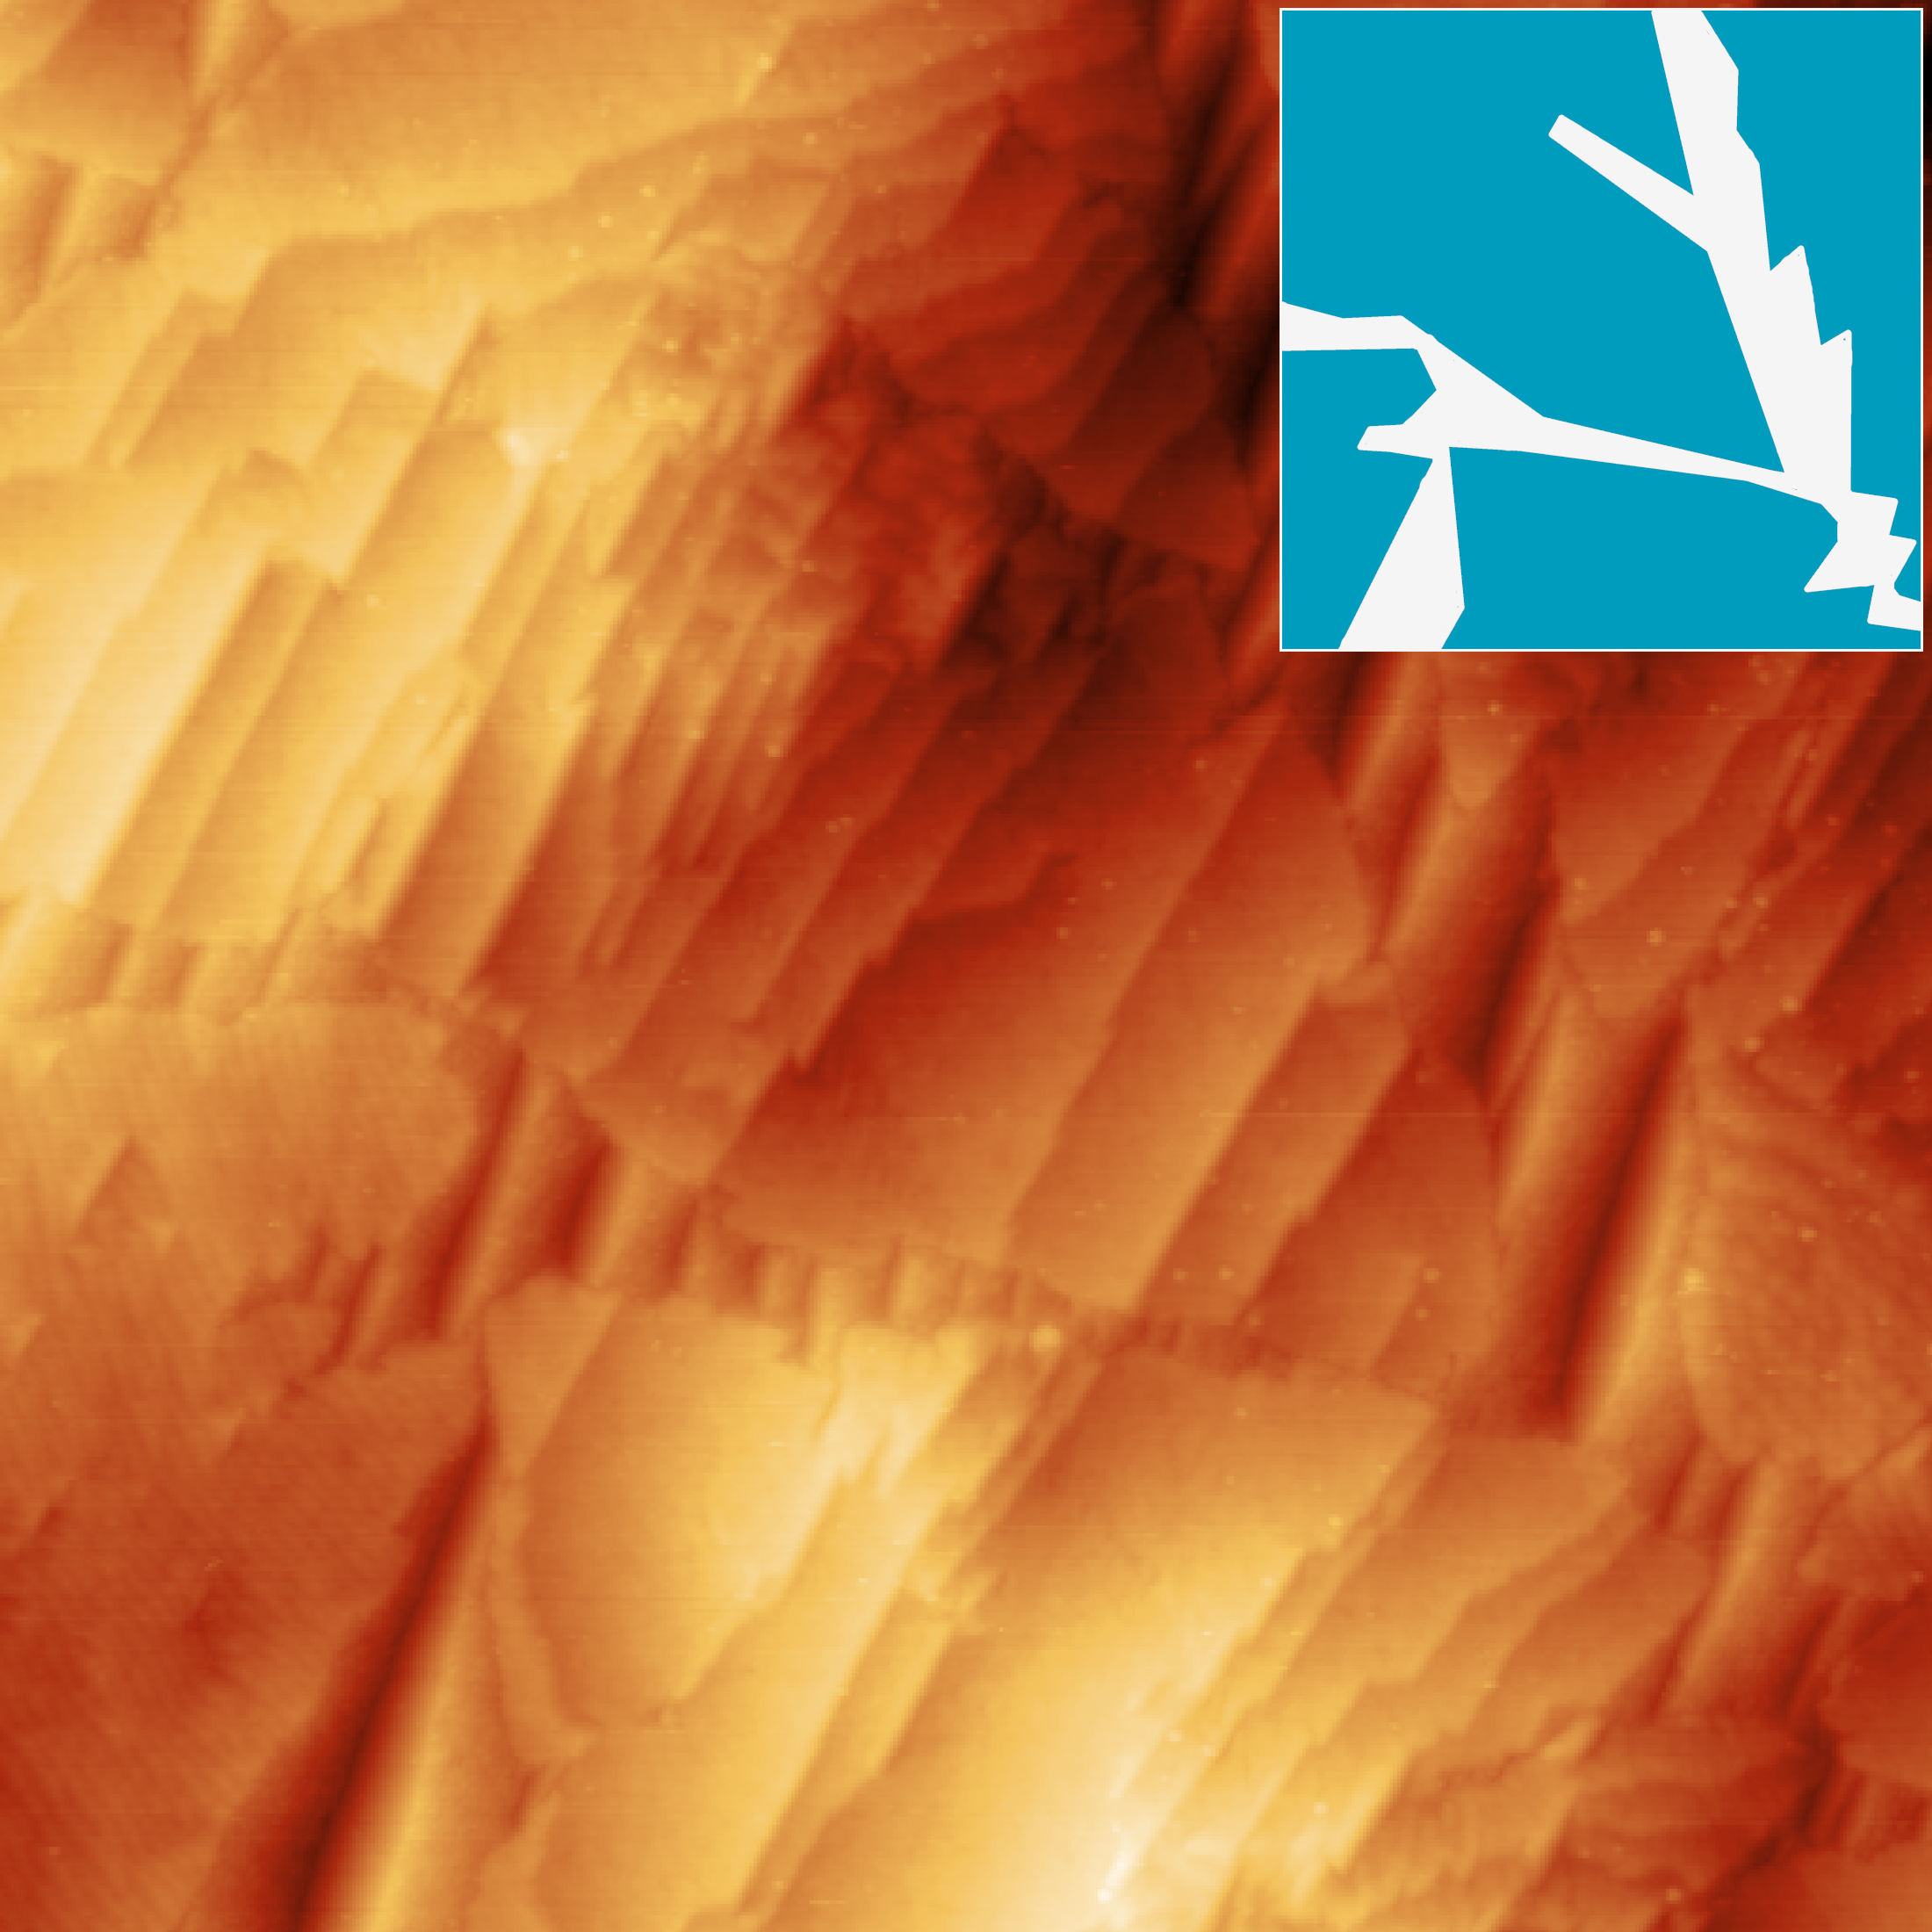
\includegraphics[width=0.7\textwidth]{./images/F150423-102732-with-inset}
	% \caption{}
	%\end{figure}
	%%%%%%%%%%%%%%%%%%%%%%%%%%%%%%%%%%%%%%%%%%%%%%%%%%%%%%%%%%%%%%%%%%%%%%%%%%%%%%%%%%%%%%%%%%
	%\begin{figure}
	% \centering
	%\subfigure[]{%
	%	\includegraphics[width=0.45\textwidth]{./images/F150416-192611-detail1.png}
	%	\label{fig:h-bn-overgrown-cu-1}
	%} \quad %
	%\subfigure[]{%
	%	\includegraphics[width=0.45\textwidth]{./images/F150423-114214.jpg} 
	% 	\label{fig:h-bn-overgrown-cu-2}
	%}%
	%\caption{STM topographies of \textit{h}-BN islands that overgrow Cu-foil facets. Imaging parameters: 		
	% 	\subref{fig:h-bn-overgrown-cu-1} 
	% 		\SI{1}{\volt}, \SI{0.37}{\nano\ampere}, 
	% 		color scale \SIrange{0}{1.5}{\nano \meter}, 
	% 		Image width: \SI{18}{\nano \meter}, 
	% 	\subref{fig:h-bn-overgrown-cu-2} 
	% 		\SI{3.5}{\volt}, \SI{0.5}{\nano\ampere}, 
	% 		color scale \SIrange{0}{4}{\nano \meter}, 
	% 		Image width: \SI{73,8}{\nano \meter}. 
	%}%
	%\label{fig:h-bn-overgrown-cu}
	%\end{figure}
	
	\begin{figure}[h!]
		\centering
		\subfigure[STM topography]{%
			\includegraphics[width=0.45\textwidth]{./images/F150423-102732}
			\label{fig:h-bn-22L}
		} \quad %
		\subfigure[Color highlighted \textit{h}-BN areas]{%
			\includegraphics[width=0.45\textwidth]{./images/F150423-102732-overlayed-II} 
			\label{fig:h-bn-22L-2}
		}%
		\caption{STM topographies of \textit{h}-BN islands that overgrow Cu-foil facets. Imaging parameters: 		
			\SI{4.7}{\volt}, \SI{0.2}{\nano\ampere}, color scale \SIrange{0}{7}{\nano\meter}, Image width: \SI{295}{\nano \meter}
		}%
		\label{fig:h-bn-overgrown-cu}
	\end{figure}
	%%%%%%%%%%%%%%%%%%%%%%%%%%%%%%%%%%%%%%%%%%%%%%%%%%%%%%%%%%%%%%%%%%%%%%%%%%%%%%%%%%%%%%%%%%
\autoref{fig:h-bn-overgrown-cu} shows an area with sub-ML \textit{h}-BN coverage. As an guide to the eye, the \textit{h}-BN islands are overlaid with a blueish hue in \autoref{fig:h-bn-22L-2}. In between flat, triangular \textit{h}-BN domains the faceted copper surface can be seen.

It is apparent that the surface structure changes between free copper and \textit{h}-BN regions. While the facets are clearly visible on free copper areas, the overgrowing \textit{h}-BN creates a new surface where the faceted copper surface is not visible anymore. In most of the overgrown areas wider terraces are formed that are divided by almost straight step edges that roughly follow the facets orientation.

Different \textit{h}-BN structures are visible in \autoref{fig:h-bn-22L}. While most islands (I) do not show much internal structure, some (II) show some apparent height variations in STM. They overgrow the facets and mask their height profile like the structure-less islands but terraces are connected by unregular shaped step edges. These typically do not follow facet orientation and two neighboring terraces are separated by a smaller height difference.  No relation between island orientation and type (I / II) can be found.

The surface structure is varying across the image. Regions with square (top left corner) and hexagonal (center) symmetric step edges are found in close proximity but only occur below overgrown areas for island type (I). 

Height profiles are taken for several facets. The angle between rising and falling facet fronts is compared with typical facet angles at single crystal surfaces but no clear assignment can be done. Higher order facet orientations are discussed in \autoref{fig:step-heights}. The facet orientation varies slightly across the image. 

%%%%%%%%%%%%%%%%%%%%%%%%%%%%%
\FloatBarrier
%%%%%%%%%%%%%%%%%%%%%%%%%%%%%

\subsection{XPS characterization}
%this file contains information on self-grown \textit{h}-BN on the comercially bought copper foils
%Copper foils with \SI{0.25}{\mm} were bought and repeatedly sputtered/annealed. Several grow cycles of \textit{h}-BN via CVD of borazine were done.  
The sample is transferred to the XPS-STM chamber and again sputtered/annealed several times to clean it properly.

The needed dosage of borazine to assemble a full mono layer of \textit{h}-BN is derived via a combined STM/XPS measurement. Several preparations were done to understand the growth behavior of \textit{h}-BN on the copper foil. Coverage is measured in STM while the chemical composition of the sample was assessed with XPS.

\begin{table}[h!]
	\centering
	\caption{Determination of the full mono layer borazine dosage. First a saturated sample was prepared (I) and measured in XPS/STM. A sub-mono layer (II) was grown and compared to the monolayer STM and XPS results.}
	\begin{tabular}{cccccccc}
		& Prep. & Position    & Area [arb.u.] & FWHM  & Anode & Dosage  & Coverage\\ 
		&	  &	[eV]	& (XPS)		&[eV]	&Element&[L]	  & (STM) \\ \hline \hline
		\multirow{2}{*}{B1s} 	&I& 191.1 & 3776 & 1.35 & Mg & 4736 & \SI{100}{\percent}\\
		&II& 191.1 & 1994 & 1.35 & Mg & 789 &\SI{53}{\percent}\\ \hline
		\multirow{2}{*}{N1s} 	&I& 398.7 & 5875 & 1.45 & Al  & 4736 & \SI{100}{\percent}\\
		&II& 398.6 & 3183 & 1.43 & Al & 789 &\SI{54}{\percent}\\
	\end{tabular}
\end{table}

%\begin{figure}[ht]
%	\centering
%	\subfigure[N1s]{
%		\includegraphics[width=.45\textwidth]{./images/XPS-150314-N1s.jpg}
%	}
%	\subfigure[B1s]{
%		\includegraphics[width=.45\textwidth]{./images/XPS-150314-B1s.jpg}
%	}
%	\subfigure[C1s]{
%		\includegraphics[width=.45\textwidth]{./images/XPS-150314-C1s.jpg}
%	}
%	\subfigure[Cu3s]{
%		\includegraphics[width=.45\textwidth]{./images/XPS-150314-Cu3s.jpg}
%	}
%	\caption{\textbf{REDO! Axis too small!! Check layout with other XPS measurements!!} XPS spectra for ML \textit{h}-BN/Cu-foil. The peaks are at their expected positions\cite{kidambi_situ_2014} and show no additional features. No remnants of sulfur or remaining oxygen could be found.}
%	\label{fig:xps-self-grown}
%\end{figure}

\begin{figure}[!h]
	\centering
	\subfigure{
		\includegraphics[width=.22\textwidth]{./images/N1s-prepared}
	}
	\subfigure{
		\includegraphics[width=.22\textwidth]{./images/B1s-prepared}
	}
	\subfigure{
		\includegraphics[width=.22\textwidth]{./images/C1s-prepared}
	}
	\subfigure{
		\includegraphics[width=.22\textwidth]{./images/O1s-prepared}
	}
	\caption{XPS spectra for ML \textit{h}-BN/Cu-foil. The peaks are at their expected positions\cite{kidambi_situ_2014} and show no additional features. No remnants of sulfur or remaining oxygen could be found.}
	\label{fig:xps-self-grown}
\end{figure}

When comparing the resulting coverage (STM coverage/XPS signal) (II) to the (saturated) mono layer (I) one can derive the minimal amount of borazine needed to process a mono layer of \textit{h}-BN on the copper foil. Comparing the coverages of a sample grown with CVD, \SI{7E-6}{\milli \bar} for 15min (I) and one grown with CVD, \SI{3.5E-6}{\milli \bar} for 5min (II), shows that reducing the dosage by a factor of 6 does not reduce the coverage by a factor of 6, but instead by a factor of 2. Therefore (I) features a full monolayer and (II) only half of it. It follows that a full monolayer may be achieved by dosing at least \SI{1500}{\langmuir} borazine on a \SI{800}{\degreeCelsius} hot copper foil surface. 
Because the growth rate may certainly not be linear (less and less free copper surface to decompose borazine into building fragments while the layer assembles) the given dosage is a minimum estimation to achieve the mono layer.

Even though a much larger amount for borazine (\SI{4736}{\langmuir}) than needed for a mono layer (\SI{1500}{\langmuir}) has been dosed, the maximum coverage did not exeed ne XPS signal of a mono layer. So the growth of \textit{h}-BN on copper foil is self-limited (as in the case of many \textit{h}-BN/metal systems) to a full mono layer. It is not possible to achieve layer growth with this type of preparation.

T and t dependence is not subject to investigation because the growth is supposed to follow the same mechanisms as on the single-crystal case. Quiet some investigation has been done, \cite{orlando_epitaxial_2012,preobrajenski_monolayer_2007-1} to understand this process.

\subsubsection{Commercial \textit{h}-BN sample}
\label{sec:commercial-hBN-XPS}
The quality of the as-bought \textit{h}-BN on copper foils\cite{_graphene_2014} is examined in XPS. Results are shown in \autoref{fig:xps-bought}.
%%%%%%%%%%%%%%%%%%%%%%%%%%%% make it better looking? %%%%%%%%%%%%%%%%%%%%%%%%%%%%%%%%%%%%%
\begin{figure}[!h]
	\centering
	\subfigure{
		\includegraphics[width=.22\textwidth]{./images/N1s-bought}
	}
	\subfigure{
		\includegraphics[width=.22\textwidth]{./images/B1s-bought}
	}
	\subfigure{
		\includegraphics[width=.22\textwidth]{./images/C1s-bought}
	}
	\subfigure{
		\includegraphics[width=.22\textwidth]{./images/O1s-bought}
	}
	\caption{XPS spectra of as-bought \textit{h}-BN/Cu-foil sample\cite{_graphene_2014}. All spectra are taken at room temperature in as-bought state (black) and after annealing to \SI{630}{\K} (blue) and \SI{970}{\K} (red).}
	\label{fig:xps-bought}
\end{figure}

%
%\begin{landscape}
%	\begin{figure}
%		\includegraphics[angle=0,width=1.2\textwidth]{./images/XPS-spectra-as-bought.pdf}
%		\caption{}
%	\end{figure}
%\end{landscape}	

The XPS spectra shows contribution of different atomic species. There are peaks for the O-atoms (1s: \SIrange{529}{535}{\eV})), C-atoms (1s $\approx \SI{285}{\eV}$), N-atoms (1s $\approx \SI{398}{\eV}$), B-atoms (1s $\approx \SI{190}{\eV}$) and Cu-atoms ($3p_{1/2,3/2}$: \SIrange{70}{80}{\eV})). One would expect the shape of the 1s-peaks to be singlet-like (one peak, gauss shaped) and the 3p-peak to be a doublet (two close lying peaks with area-ratio 1/2:3/2=1:2).

There are different oxygen containing species expected to be present on the unprepared sample surface, including $CO$/$CO_2$, $CuO$/$Cu_2O$ and $H_2O$. They are possible surface contaminants due to sample storage under atmospheric conditions.
\paragraph{O1s}
Position varies with temperature. The signal at room temperature(black) stems from adsorbed water and CO. These desorb with increasing temperature(blue). When going to higher temperatures(red) this peak increases again and shifts to higher binding energies. Not present in self-grown \textit{h}-BN (\autoref{fig:xps-self-grown})

\paragraph{C1s}
The C1s Peak decreases with increasing temperature and retains its position. This has the same  reason as for the O1s peak (desorption of CO due to the heating). Some of the carbon remains on the surface - even at temperatures as high as \SI{970}{\K}.

\paragraph{N1s/B1s}
The nitrogen/boron peaks show some temperature related changes. There is little change upon annealing to \SI{630}{\K}, both peaks shrink, but stay almost constant in their position in binding energy (sightly shifted to lower binding energies by about \SI{0.2}{\eV}). Position is [N1s: \SI{398.1}{\eV} | B1s: \SI{190.2}{\eV}]. Further annealing leads to a intensity decrease.

\paragraph{Cu3p}
The copper peak exhibits an increase in area when increasing the temperature. This is because some of the water and CO adsorbate desorb and more and more copper is contributing to the signal. This peak is a doublet, so both signals come from the same chemical copper surrounding.


The $Cu(OH)_2$ O1s peak is expected to be at \SIrange{531.3}{531.7}{\eV}\cite{deroubaix_x-ray_1992} which may explain the shoulder of the O1s peak to higher binding energies (O\textit{1s} metal: \SI{531}{\eV}). Nitrates ($NO_3$) have binding energies in the range from \SIrange{532.5}{533.5}{\eV}\cite[45]{wanger_handbook_1979}. This would imply either an replacement of nitrogen with oxygen, or some kind of oxygen on top or below the the BN layer. As proven by Simonov et al. in \cite{simonov_controllable_2012} the atomic oxygen tends to replace the nitrogen in the \textit{h}-BN/Ir(111) system when it is annealed to \SI{600}{\degreeCelsius}. Thus it forms $B_{x}N_{y}O_{1-x-y}$ over-layers. The longer the oxidation time the higher the amount of replaced nitrogen. 

If this effect is responsible for the O\textit{1s} peak at high temperatures is questionable, since the oxygen has to be cracked somehow - where no process can be thought of (no catalytic cracking at metal surface possible - full ML, thermal energy to low to reach binding energies of $O_2$.

\textbf{An exchange of O with B or N would be easily visible in XPS (due to changed N/B surroundings. Not sure if the signal of oxygen is large enough for that.}

\subsection{Application: Molecular adsoprtion of TPCN}
\label{sec:foil-use-case}

\begin{wrapfigure}{r}{5cm}\centering
	\includegraphics[width=5cm]{./images/molecules/TPCN-scalebar}
	\caption{TPCN}
	\label{fig:TPCN-scalebar}
\end{wrapfigure}

To test the use of polycrystalline copper foils in molecular adsorption experiments, the Cu(111) support for the \textit{h}-BN growth is replaced by a polycrystalline copper foil. The \textit{h}-BN layer has been prepared by a dose of \SI{5E-7}{\milli\bar} borazine for \SI{20}{\min} (\SI{4500}{\L}) at the LT-STM chamber. During dosage the foil has been kept at \SI{820}{\celsius}. 

Here carbonitrile-functionalized porphyrin (2H-TPCN) molecules are used as molecular building blocks, as these have been studied in the past with single crystalline supports.\cite{urgel_controlling_2015} After Co dosage they show regular metal-organic coordination networks on \textit{h}-BN/Cu(111).
%  
%  When a \textit{h}-BN spacer layer is introduced, the molecules decouple from the substrate, lowering their interaction with the afore-mentioned. This can be seen in a change of the molecules' footprint (rectangular $\rightarrow$ square ).
%  
%  They do not form ordered networks (like chains or squares) and lie rather loosely on the \textit{h}-BN layer (\textcolor{red}{\textbf{compare 150807.142226.dat}}). They can easily be moved with the STM tip (\SI{1}{\volt}, \SI{10}{\nano \ampere}). In some areas, denser TPCN islands form. Here they lie right next to each other, slightly shifted to match the neighboring molecules and to achieve the dense packed regions. The same motif was already investigated in the same system \cite{urgel_controlling_2015}, hardening the assumption of a decoupling \textit{h}-BN layer.
%  
%  During scanning ($I=\SI{0.1}{\nA},\ \SI{0.9}{\V}<U<\SI{1.3}{\V}$) of a group of molecules, a single molecule could be pushed out of the group (compare figure \autoref{fig:TPCN-manipulation} in appendix). While the chain initially consisted of 3 molecules in a row, after scanning one of the molecular units moved to the left while the remaining two stay at their positions. A closer look to the moved molecule's geometry reveals deformation of the legs.\textcolor{red}{\textbf{More information or don't mention?}}
%  
%  It was shown that the imminic nitrogen species within a 2H-TPP molecule strongly interact a Cu(111) surface, thus orient along high symmetry directions.\cite{haq_clean_2011, buchner_diffusion_2011, gonzalez-moreno_following_2011, diller_self-metalation_2012, ditze_activation_2012,rojas_self-assembly_2010} 
%  Rotation and diffusion are limited. \textcolor{red}{\textbf{What does this tell me? Molecules on Cu(111) are all oriented the same or rotated by \SI{90}{\degree} or \SI{60}{\degree}? Thats a $\pm$ \SI{30}{\degree}}}
% 
% TPCN without added cobalt form similar pattern on the \textit{h}-BN/Cu-foil system (compare fig. 2b in \cite{urgel_controlling_2015}). Although the ordered areas were quiet rare, an arranged region has been found. Here the molecules are not strictly equidistant or -rotated which makes it difficult to give an accurate unit cell for this type of motif.
%  %--------- Describe how the TPCN form that network on h-BN --------- 

\begin{figure}[!h]
	\centering%
	%  	\subfigure[Zoomed view ($\SI{10}\times\SI{10}{\square\nm}$)]{
	%  		\includegraphics[width=0.45\textwidth]{./images/F150814-090450_01}
	%  	}
	%  	\subfigure[($\SI{20}\times\SI{35}{\square\nm}$)]{
	%  		\includegraphics[width=0.45\textwidth]{./images/F150814-090305-cut1}
	%	  	\label{fig:TPCN+Co-STM-large}
	%  	}
	%
	\subfigure[Image width: $\SI{22}\times\SI{17}{\square\nm}$, Color scale \SIrange{0}{2}{\nano \meter}]{
		\includegraphics[width=0.9\textwidth]{./images/F150814_090305_cut1-new-overlay}
		\label{fig:TPCN+Co-STM-large}
	}
	\subfigure[Image width: \SI{10}{\nano \meter}, Color scale \SIrange{0}{1}{\nano \meter}]{
		\includegraphics[width=0.42\textwidth]{./images/F150814_090305_cut2}
		\label{fig:TPCN+Co-STM-small}
	} \quad
	\subfigure[Model]{
		\includegraphics[angle=90,width=0.42\textwidth]{./images/F150814-090305-cut2-new}
		\label{fig:TPCN+Co-STM-small-model}
	}
	\caption{Self-Assembled TPCN molecules after Co adsorption on \textit{h}-BN/Cu-foil. Two moir\'e hills are partially visible in \subref{fig:TPCN+Co-STM-large}, imaged at \SI{4.46}{\volt}, \SI{0.04}{\nano\ampere}. \subref{fig:TPCN+Co-STM-small-model} The cobalt atoms sit in between the TPCN molecules and facilitate a regular, ordered arrangement. The unit cell is shown as black square. Two defects are visible.}%
	\label{fig:TPCN+Co-STM}%
\end{figure}%

Unveiling the structure of the island beginning at its edges shows the orientation and lateral position of the molecules which is highlighted by dashed outlines in \autoref{fig:TPCN+Co-STM-large}. The molecular center is shown in black while the leg functionalization is shown in blue.

The molecules form a regular 2D network and arrange in a square unit cell with center-center distances of \SI{2.43 \pm 0.05}{\nano \meter}. All molecules within are rotated the same and connected by their CN functions via Co atoms. 

A Co atom connecting two neighboring molecules via their legs results in a distance of \SI{2.81 \pm 0.05}{\angstrom} between the N terminated leg and Co atom. Typical binding distances for Co-NC are reported \cite{schlickum_metalorganic_2007, przychodzen_supramolecular_2006} and in good agreement.

Two defects are visible in \autoref{fig:TPCN+Co-STM-small} as depressions in the otherwise regular cobalt lattice connecting the molecules. A missing Co atom leads to a symmetric, cross like depression in the apparent height. The four protrusions resemble the shape of intact functional groups.

A defect asymmetric in shape is visible in the lower half of \autoref{fig:TPCN+Co-STM-small}. Here the connection between four molecules is distorted. While three of four legs appear regular in shape and point to the central cobalt atom, a single leg appears different. This is attributed to an altered function of the leg, likely due to the loss of the pyridil group.

Few signs for porphyrin center metalization, neither many access cobalt ad atoms (additional bright spots in between the molecular assembly) are observed. 

The same mechanisms are present for 2H-TPCN/\textit{h}-BN/Cu(111)+Co \cite{urgel_controlling_2015} and show the resemblance of \textit{h}-BN grown on Cu(111) and polycrystalline copper foils as molecular assembly support.

\section{Summary \& Outlook}
  \begin{itemize}
	\item Look at Messzeit-April.ppt power point presentation
	\item Stufenh\"ohe
	\item Warum sehe ich kein moir\'e? Spannungsabhängigkeit [4V/1V] siehe 121542
\end{itemize}

The surface roughness of polycrystalline copper foils has been improved with the chemical polish approach. After polishing the foil a decrease in surface roughness of about \SI{50}{\percent} is achieved. After several sputter and annealing cycles, \textit{h}-BN can be grown on alike prepared foils. The quality of the grown \textit{h}-BN is good and allows for molecular adsorption experiments, that reproduce experimental results on \textit{h}-BN grown on Cu(111) as tested for TPCN + Co.

The prepared \textit{h}-BN/Cu-foils were compared to bought \textit{h}-BN/Cu-foils in XPS experiments. For the commercial available samples the binding energy for nitrogen and boron is lower by $\approx \SI{500}{\milli \eV}$. Both show carbon peaks. While the C\textit{1s} signal for the experimentally prepared sample is small, it is considerable for the bought samples and could not completely be removed via gentle heating. For the bought samples oxygen contamination is present and annealing did not show a complete removal of the contaminants.

Some foil has been mechanically polished with 4k paper and several hours of Syton polishing. The roughness of these samples has been investigated in AFM, too. It is comparable to the chemically polished ones, but always larger by $\approx \SI{10}{\percent}$. Sometimes unwanted new scratches appear after mechanical polish.

To further improve the quality of the foil, one could follow the documented recipe for annealing the foil in a $H_2$ atmosphere (\SI{10}{sscm}, \SI{1000}{\celsius}, 30min)\cite{kim_synthesis_2012} to increase the copper grain size and further smoothen the surface. 

\chapter{Bis- \& Tetra-pyridin-4-ylethynyl functionalized pyrene molecules on \textit{h}-BN\/Cu(111)}
\subsection{Abstract}
The position and number of functional groups of pyridin-4-ylethynyl functionalized pyrene molecules control their self-assembly and electronic properties. To access these in UHV, decoupling of the underlying substrate (Cu(111)) is mandatory and achieved here with a \textit{h}-BN spacer layer. As a result unperturbed HOMO and LUMO states are resolved in STM. While STS shows a band gap that decreases with increasing number of functional groups, it is not affected by their position and the molecular assembly observed STM. The gap between pronounced HOMO/LUMO states is modulated by the electronically corrugated \textit{h}-BN/Cu(111) interface and predominantly determined by the larger shift of the LUMO states. UV/Vis measurements in solution reveal a high quantum yield of the fluorescence emission at wavelengths consistent with ab-initio DFT calculations. Finally, the ability of trans-pyrene to act as host system for cis-pyrene is shown.

\subsection{Introduction}
Pyrene’s optical properties\cite{Figueira-Duarte_Pyrene_2011} make it a promising candidate for potential applications. 1,3,6,8-tetrasubstituted pyrenes are used in a variety of applications, including blue\cite{Moorthy_Steric_2007,Sonar_pyrenes_2010,Feng_Pyrene_2012}, yellow\cite{Sonar_pyrenes_2010}, green\cite{Chang_efficient_2012} and multilayered\cite{Thomas_pyrene_2012} OLEDs. The emergence of these compounds in applications is based on fundamental research in (not only, but including) surface science conducted under conditions where unperturbed photophysical properties of the molecule can be controlled and tuned. Optical properties are often investigated on transparent insulating bulk materials (Differential Reflectance Spectroscopy (DRS) - PTCDA/mica)\cite{Proehl_Formation_2004}, (Reflectance anisotropy spectroscopy - $\alpha$-quaterthiophene/potassium hydrogen phthalate)\cite{Bussetti_reflectance_2009} but are also possible on nontransparent HOPG(photoluminescence - quater – (4T) and sexithiophene (6T) films/HOPG)\cite{Schneider_Morphology_2002} or SiO2 (pentacene, perfluoropentacene, and diindenoperylene/SiO2)\cite{Heinemeyer_Real-Time_2010} surfaces. These space averaging techniques are complemented with measurements on atomic length scales where sub-molecular topographic and electronic structure are investigated by STM and STS in UHV. These need a conducting support for the molecules to adsorb on, making the choice of a suitable substrate important.
Molecules adsorbed on metal surfaces interact with their support, resulting in luminescence quenching (Photoluminescence - Quaterthiophene and PTCDA on Ag(111))\cite{Gebauer_Luminescence_2004} and broadened frontier molecular orbitals. Mediated by the presence of a metal, these exhibit considerable interaction with low-lying orbitals, changing their shape\cite{Chavy_Interpretation_1993}. To minimize the interaction with a metallic substrate, spacer layers of insulating materials are used. 
Recent years of research have increased the variety of these while a continuous decrease in layer thickness could be achieved. For example, ultrathin (~6) layers of NaCl (pentacene/NaCl)\cite{Repp_molecules_2005} and KCl\cite{Koslowski_adsorption_2017} are utilized for direct imaging of unperturbed molecular orbitals in STM. The thinnest spacer (since it consists only of a single layer of atoms) is provided by a \textit{h}-BN monolayer. Its large band gap is used to minimize interaction with the metallic substrate as shown experimentally\cite{joshi_boron_2012} and theoretically (DFT – silicene/\textit{h}-BN/Cu(111))\cite{Kanno_Electronic_2014}. Here self-assembly and electronic properties can be studied in STM/STS and compared with other unperturbed systems as well as with theory. 
In this work we propose functionalized pyrene building-blocks\cite{Casas-Solvas_Synthesis_2014,Feng_Functionalization_2016} for self-assembled regular molecular arrays on surfaces. Functionalization with pyridin-4-ylethynyl\cite{Figueira-Duarte_Pyrene_2011} makes pyrene an versatile agent for controlled self-assembly. Cis- , trans- and tetra functionalized pyridin-4-ylethynyl-pyrene was already investigated on Ag(111) system resulting in one-dimensional coordination chains, two-dimensional arrays and chiral, porous kagom\'e networks, where assembly is controlled by the number and position of substituents.\cite{Kaposi_Supramolecular_2016} 
Hereinafter the influences of self-assembly, leg functionalization\cite{Kurata_donor_2017} and intra moir\'e position\cite{Sushobhan_Control_2014} on the band gap is investigated. Mandatory electronic decoupling is achieved either on \textit{h}-BN/Cu(111) or in solution where the molecules’ density of states is not influenced by a supporting metal.

\subsection{Results}

We investigate three different derivatives of pyridin-4-ylethynyl substituted pyrenes shown in \autoref{fig:pyrene-fig1}: \subref{fig:pyrene-fig1-tetra} Tetra-pyrene has four functional groups added at position 1,4,6 and 8. The point symmetric result is therefore neither chiral nor bears a dipole moment. \subref{fig:pyrene-fig1-trans} Trans-pyrene is substituted at the positions 1 and 6 (“equatorial” positions) resulting in a pro-chiral molecule. \subref{fig:pyrene-fig1-cis} Cis-pyrene is functionalized at longitudinal positions 1 and 8. With both electron rich groups being on the same side, they create a permanent dipole moment of 4.1 D in this non-chiral molecule.

\begin{figure}[b] \centering
\subfigure[]{
		\includegraphics[width=0.25\textwidth]{./images/paper/pyrene/tetra-model}
		\label{fig:pyrene-fig1-tetra}
	}
\subfigure[]{
		\includegraphics[width=0.25\textwidth]{./images/paper/pyrene/trans-model}
		\label{fig:pyrene-fig1-trans}
	}
\subfigure[]{
		\includegraphics[width=0.25\textwidth]{./images/paper/pyrene/cis-model}
		\label{fig:pyrene-fig1-cis}
	}
	\caption{AM1 relaxed functionalized pyrene species in gas phase. Structure of \subref{fig:pyrene-fig1-tetra} tetra-, \subref{fig:pyrene-fig1-trans} trans- and \subref{fig:pyrene-fig1-cis} cis-pyridil functionalized pyrene molecule. All species are virtually flat.}
	\label{fig:pyrene-fig1}
\end{figure}

The 4-ylethynyl functionalization leads to a certain degree of freedom to rotate the group in plane or tilt the pyridil ring around the C-C bond connecting it to the rigid pyrene core (compare appendix S13).


\begin{figure}[] \centering
	\includegraphics[width=0.7\textwidth]{./images/paper/pyrene/figure-2}
	\caption{Schematic drawing of the frontier Kohn−Sham orbitals for trans- \& tetra-pyridil-ethynyl substituted pyrene derivatives, together with orbital correlation diagram in comparison of the molecular orbitals (MOs) for pyrene itself, at the B3LYP/6-31G** level of DFT.}
	\label{fig:pyrene-fig2}
\end{figure}

To evaluate the effect of the substitution on the pyrene core DFT calculations were performed (B3LYP/6-31G** level of theory, in vacuum). The frontier Kohn-Sham orbitals of pyrene and di- and tetra-substituted pyridylethynyl pyrene are shown in \autoref{fig:pyrene-fig2} and \autoref{fig:pyrene-S4}, \autoref{fig:pyrene-S8}.
These show that pyrenes have large orbital coefficients at the 1-, 3-, 6- and 8-positions, with the nodal plane going through the 2- and 7- positions.\cite{Kurata_donor_2017,Maeda_Alkynylpyrenes_2006,Diring_Luminescent_2009,Crawford_experimental_2011,Ji_Electron_2015,Lee_Enhanced_2012} Consequently, orbital interactions between the pyrene and the pyridylethynyl MOs have an effect on stabilizing the highest occupied (HOMO) and lowest unoccupied (LUMO) molecular orbital energy levels. While the HOMO stabilization plays only a small part, the considerable lowering of the LUMO energy levels lead to smaller HOMO-LUMO gaps. The picture of orbital interactions is similar in cis- and tetra-pyrene, with the HOMO-LUMO gap being influenced mostly by the number of substituents: The gap of tetra-substituted pyrene (\SI{2.54}{\eV}) becomes narrower than that of bi-substituted trans-pyrene (\SI{2.95}{\eV}), which is in accordance to experimental findings (vide infra) and previous literature reports.\cite{Maeda_Alkynylpyrenes_2006, Diring_Luminescent_2009, Lee_Enhanced_2012}
%%%
As both the electronic and optical properties of molecules are quenched or at least altered upon adsorption on metal surfaces it is necessary to decouple the functional pyrenes from the metallic substrate. Therefor we grow a single layer of \textit{h}-BN on a Cu(111) single crystal. Besides its insulating properties we have chosen this lattice mismatched system (\textbf{citation}) to make use of its spatially modulated surface potential (\textbf{citation}). Depending on the registry of adsorbate (B, N) and substrate (Cu) atoms the surface is divided in regions of larger (pore) and lower (wire) work function. This moir\'e is used here to fine tune the energy of molecular states.
When choosing a bias voltage close to the onset of the LUMO one can easily note molecules in the pore region already contributing to the tunneling current resulting in a bright protrusion in STM although \textit{h}-BN/Cu(111) forms a weakly corrugated layer (\textbf{citation}). 

After deposition tetra-pyrene molecules assemble in dense packed islands shown in \autoref{fig:pyrene-fig3}. Every molecule within the island shows the same orientation. The unit cell is triclinic (\SI{1.63}{\nano \meter} $\times$ \SI{1.50}{\nano \meter}, \SI{92}{\degree}) and holds a single molecule. The binding motif is guided by the functional groups where a pyridil ring forms a bond with the adjacent pyridil ring of the neighboring molecule. Assuming flat pyridil groups parallel to the surface, the assembly is characterized by two intermolecular distances $d_1$ and $d_2$ between two pyridil groups, $d_1$ ($d_2$) pointing to the long (short) side of the pyrene core as indicated by black lines connecting neighboring nitrogen and hydrogen termini in the inset of \autoref{fig:pyrene-fig3b}. 

\begin{figure}[] \centering
	\subfigure[]{
		\includegraphics[width=0.7\textwidth]{./images/paper/pyrene/figure-3a}
		\label{fig:pyrene-fig3a}
	}
	\subfigure[]{
		\includegraphics[width=0.7\textwidth]{./images/paper/pyrene/figure-3b}
		\label{fig:pyrene-fig3b}
	}
	\caption{STM topography of tetra-pyrene adsorbed on \textit{h}-BN/Cu(111). \subref{fig:pyrene-fig3a} Hexagonal moir\'e superstructure visible as bright protrusions. \subref{fig:pyrene-fig3b} After RT deposition the molecules assemble in dense packed islands in a square unit cell (black square). Molecular model superimposed. Inset (\SI{2}{\nano \meter} $\times$ \SI{2}{\nano \meter}) shows inter molecular distances $d_1$ and $d_2$. 
		Imaging parameters: 
		\subref{fig:pyrene-fig3a} \SI{2}{\volt}, \SI{0.1}{\nano \ampere}, \textcolor{red}{Image width:} and 
		\subref{fig:pyrene-fig3b} \SI{0.1}{\volt}, \SI{0.2}{\nano \ampere}, \textcolor{red}{Image width:}
	}
	\label{fig:pyrene-fig3}
\end{figure}

$d_1$ and $d_2$ equal \SI{0.288}{\nano \meter} and \SI{0.254}{\nano \meter} respectively and are both comparable to experimental\cite[5]{Kaposi_Supramolecular_2016} (\SI{0.27 \pm 0.05}{\nano \meter}) and theoretical\cite[5]{Arras_Nature_2012} (\SI{0.27}{\nano \meter}) results (\textcolor{red}{\textbf{find more of those!}}). Though hard to address quantitatively in STM a small tilt of the pyridil termini is likely present to compensate for the close proximity of the H-terminated pyridil rings and is observed as minor contrast differences within the four legs of the molecule. This tilt may enable interactions between the N terminated pyridil group and the pi system of the neighboring pyridil group, giving rise to an additional binding component beside a strict N-H hydrogen bonding.

%%
In addition to the topographic structure, STS reveals the electronic structure of the assembly. All spectra shown in \autoref{fig:pyrene-fig4b} are taken on the center of a molecule. Colored spectra and points (\autoref{fig:pyrene-fig4a}) indicate their distance to the \textit{h}-BN pore that is recognized as bright protrusion in \autoref{fig:pyrene-fig4b}. The darker the color of the points/spectra the larger the lateral distance to the pore. Molecular orbital energies are indicated by yellow (HOMO) and blue (LUMO) boxes. A blue arrow illustrates the electronic gap between both. Spectra have been fitted with a gauss function after background subtraction to determine the corresponding electronic states. The energy onset of HOMO is located between \SIrange{-1541}{-1583}{\milli \volt} with a dependence on the position within the moir\'e unit cell of 42 mV. The LUMO emerges at 
\SIrange{886}{1198}{\milli \volt}
%(886 ± 1) – (1198 ± 1) mV, 
with a notable shift of \SI{312}{\milli \volt} that compares well to the reported change in work function of the \textit{h}-BN/Cu(111) substrate.\cite{Sushobhan_Control_2014,Liu_Interplay_2015,Schulz_Templated_2013,urgel_controlling_2015} This is in good agreement with literature reporting different level alignment for occupied and unoccupied molecular orbitals where the larger shift of the LUMO mainly determines the electronic gap. It is smaller close to the pores.\cite{Kumar_Molecular_2017} The large gap between HOMO and LUMO (\SI{2.56}{\eV}) benefits molecular orbital resolution (Figure S4) and indicates efficient decoupling from the metallic substrate due to the insulating \textit{h}-BN spacer. 

\begin{figure}[] \centering
	\subfigure[]{
	\includegraphics[height=5cm]{./images/paper/pyrene/figure-4b}
	\label{fig:pyrene-fig4b}
	}
	\subfigure[]{
		\includegraphics[height=5cm]{./images/paper/pyrene/figure-4a}
		\label{fig:pyrene-fig4a}
	}
	\caption{Spatial variation of molecular energy states within the moir\'e of tetra-pyrene. \subref{fig:pyrene-fig4a} STS on varying positions within moir\'e unit cell. HOMO and LUMO are indicated by yellow and blue boxes connected by an arrow indicating the electronic gap. A black vertical line is drawn close to the onset of LUMO+1 states at which energy the topography in \subref{fig:pyrene-fig4b}) was recorded. \subref{fig:pyrene-fig4b} STM topography where colored points indicate positions of spectra shown in \subref{fig:pyrene-fig4a}. Imaging parameter: \SI{11.07}{\nano \meter}, \SI{2.05}{\volt}, \SI{0.8}{\nano \ampere}}
	\label{fig:pyrene-fig4}
\end{figure}

In addition to the topographic structure, STS reveals the electronic structure of the assembly. All spectra shown in \autoref{fig:pyrene-fig4a} are taken on the center of a molecule. Colored spectra and points (\autoref{fig:pyrene-fig4b}) indicate their distance to the \textit{h}-BN pore that is recognized as bright protrusion in \autoref{fig:pyrene-fig4b}. The darker the color of the points/spectra the larger the lateral distance to the pore. Molecular orbital energies are indicated by yellow (HOMO) and blue (LUMO) boxes. A blue arrow illustrates the electronic gap between both. Spectra have been fitted with a gauss function after background subtraction to determine the corresponding electronic states. The energy onset of HOMO is located between \SIrange{-1541}{-1583}{\milli \volt} with a dependence on the position within the moir\'e unit cell of 42 mV. The LUMO emerges at \SIrange{886}{1198}{\milli \volt}, with a notable shift of \SI{312}{\milli \volt} that compares well to the reported change in work function of the \textit{h}-BN/Cu(111) substrate.\cite{Sushobhan_Control_2014,Liu_Interplay_2015,Schulz_Templated_2013,urgel_controlling_2015} This is in good agreement with literature reporting different level alignment for occupied and unoccupied molecular orbitals where the larger shift of the LUMO mainly determines the electronic gap. It is smaller close to the pores.\cite{Kumar_Molecular_2017} The large gap between HOMO and LUMO (\SI{2.56}{\eV}) benefits molecular orbital resolution (Figure S4) and indicates efficient decoupling from the metallic substrate due to the insulating \textit{h}-BN spacer. 

\begin{figure}[] \centering
	\subfigure[]{
		\includegraphics[width=0.7\textwidth]{./images/paper/pyrene/figure-5a}
		\label{fig:pyrene-fig5a}
	}
	\subfigure[]{
		\includegraphics[width=0.7\textwidth]{./images/paper/pyrene/figure-5b}
		\label{fig:pyrene-fig5b}
	}
	\caption{Self-assembly of trans-pyrene on \textit{h}-BN/Cu(111). \subref{fig:pyrene-fig5a} STM topography of two homo-chiral domains with minor lateral offset to each other resulting in a narrow transition region between both. \subref{fig:pyrene-fig5b} Enlarged view on one domain with overlaid models and unit cell (black rhomb). Pyridil-pyrene core connections assemble open porous networks of hexagons and triangles (kagom\'e lattice) with well-defined binding distances $d$ (black lines in inset). Image parameters: \SI{1}{\volt}, \SI{0.1}{\nano \ampere}, \textcolor{red}{Image width:\subref{fig:pyrene-fig5a}, \subref{fig:pyrene-fig5b}}}
	\label{fig:pyrene-fig5}
\end{figure}

Reducing the number of substituents by depositing trans-pyrene onto the \textit{h}-BN/Cu(111) surface results in a drastic change in assembly. Now the molecules form open porous networks with a kagom\'e pattern (citation) as shown in \autoref{fig:pyrene-fig5}. The pro-chiral character of the molecule directly translates to the on surface assembly. A result is the formation of mirror domains (Figure S9). Each of the two consist of molecules with the same chirality (homo-chiral) while no domains with mixed chirality (hetero-chiral) are observed. Although a major surface area is covered by this regular pattern, homo-chiral domains are connected by narrow intermediate regions to compensate a lateral lattice offset. The connecting region between two domains with opposite chirality is usually larger. The unit cell of the kagom\'e pattern is ?rhombic? with (3.04 x 2.93) nm long unit cell vectors and holds three molecules. The hexagonal pores feature an edge length of about 1 nm. Although not every part of the surface was regularly covered with kagom\'e patterns of either chirality, the binding motif is controlled by N-H interactions between the nitrogen in the pyridil legs and the hydrogen terminated pyrene-core of their nearest neighbor. The distance d = (0.20 ± 0.02) nm (black lines in inset of \autoref{fig:pyrene-fig5}) is smaller compared to the on reported in the dense packed assembly of tetra-pyrene and compares (how) to some literature values … … (\textbf{citation!}). The shortened binding distance builds up stress in the assembly, a reason for the limited domain size of the assembly. For the distance given above, the molecules are assumed to lie flat on the surface – including the pyridil rings. A way to release some of the adlayer stress is to increase the tilt or rotation angle of the pyridil group, both increasing the binding distance.


\begin{figure}[] \centering
	\subfigure[]{
		\includegraphics[height=5cm]{./images/paper/pyrene/figure-6b}
		\label{fig:pyrene-fig6b}
	}
	\subfigure[]{
		\includegraphics[height=5cm]{./images/paper/pyrene/figure-6a}
		\label{fig:pyrene-fig6a}
	}
	
	\caption{Spatial variation of the molecular states within the kagom\'e lattice formed by trans-pyrene on \textit{h}-BN/Cu(111). \subref{fig:pyrene-fig5a} Position and shift of HOMO (yellow) and LUMO (blue). \subref{fig:pyrene-fig5b} STM topography of a region where spectra across a moir\'e pore are taken. Colored points indicate the distance to the pores’ center. Imaging bias voltage is indicated in \subref{fig:pyrene-fig5a} by a black vertical line. Imaging parameter: \SI{11.07}{\nano \meter}, \SI{1.6}{\volt}, \SI{0.2}{\nano \ampere}
	}
	\label{fig:pyrene-fig6}
\end{figure}

To investigate the influence of the number of substituents on the electronic structure, STS is a capable technique. For trans-pyrene the HOMO in located between 
%(-1368 ± 4) and (-1490 ± 3) mV 
\SI{-1368}{\milli \volt} \& \SI{-1409}{\milli \volt}
and a LUMO between 
%(1478 ± 1) and (1816 ± 1) mV.
\SI{1478}{\milli \volt} \& \SI{1816}{\milli \volt}
 The resulting average gap between HOMO and LUMO is \SI{3051}{\milli \volt}. Molecular orbitals on pore positions of the \textit{h}-BN layer are again shifted to lower energies as compared to molecular orbitals on wire positions. The shift in LUMO energy (\SI{338}{\milli \volt}) is larger than the shift in the occupied states (\SI{122}{\milli \volt}). 
ST spectra show a large bandgap in between the HOMO and LUMO (\SI{3.05}{\eV}), which matches DFT results (\SI{2.95}{\eV}) very well. Compared to the electronic gap of the tetra-substituted species, the gap of the bis-substituted trans-pyrene is \SI{378}{\milli \volt} larger, following the trend of increasing electronic gaps with decreasing number of functional groups reflected in the DFT calculations.

\begin{figure}[] \centering
	\subfigure[]{
		\includegraphics[width=0.7\textwidth]{./images/paper/pyrene/figure-7a}
		\label{fig:pyrene-fig7a}
	}
	\subfigure[]{
		\includegraphics[width=0.7\textwidth]{./images/paper/pyrene/figure-7b}
		\label{fig:pyrene-fig7b}
	}
	\caption{Molecular self-assembly upon adsorption of cis-pyrene on \textit{h}-BN/Cu(111). White arrows indicate the preferred growth direction. \subref{fig:pyrene-fig7a} The electronic corrugation of the \textit{h}-BN (moir\'e) is visible as protrusions in LT-STM. \subref{fig:pyrene-fig7b} Overlaid molecular models of the binding motif. Unit cell is sketched as black rectangle. Enlarged inset depicts the binding distances ($d_1/d_2$) within this motif. Image parameters: \subref{fig:pyrene-fig7a} \SI{1.38}{\volt}, \SI{0.02}{\nano \ampere}, \textcolor{red}{Image width:}, \subref{fig:pyrene-fig7b} \SI{1}{\volt}, \SI{0.27}{\nano \ampere}, \textcolor{red}{Image width:}.
	}
	\label{fig:pyrene-fig7}
\end{figure}

To rule out a drastic influence of the assembly on the electronic structure we deposited cis- functionalized pyrenes. These molecules form extended, well ordered, dense packed islands, composed of rows along a preferred growth direction (compare island perimeter and white arrow in \autoref{fig:pyrene-fig7a}). Every row is composed of molecules that interconnect like tooth in a zip fastener. Molecules on one side of the fastener show the same orientation where those in the other half are rotated by \SI{180}{\degree}. The interconnection between both in shown in the inset of \autoref{fig:pyrene-fig7b} and stabilized by two bonds along $d_1$ and $d_2$. The two sides of the zip are bound via N-H binding along $d_2$ (\SI{0.298 \pm 0.01}{\nano \meter}). Within each side of the zip connection a bond between the nitrogen terminated leg and hydrogen terminated core of the trans-pyrene molecules guides chain formation along $d_1$ (\SI{0.284 \pm 0.01}{\nano \meter}, resulting in the above mentioned preferred growth direction. Stability within an island (i.e. perpendicular to the indicated growth direction) is maintained through vdW interactions of a molecules’ passivated pyrene-core to its neighbors’ with an average distance of \SI{0.26 \pm 0.05}{\nano \meter}. A unit cell within the island (black rectangle in \autoref{fig:pyrene-fig7b}, \SI{2.27}{\nano \meter} $\times$ \SI{1.57}{\nano \meter}) is made up of 2 molecules. Binding distances compare well to those present for tetra-pyrene on \textit{h}-BN where extended islands are found, too. The binding distance is comparable to those on Ag(111) as well. \cite{Kaposi_Supramolecular_2016}
The electronic structure of cis-pyrene is studied in STS. Cis-pyrene adsorbed on \textit{h}-BN (\autoref{fig:pyrene-fig8}) show a HOMO located between \SI{-1606}{\milli \volt} \& \SI{-1689}{\milli \volt} and a LUMO between \SI{1242}{\milli \volt} \& \SI{1602}{\milli \volt}. This results in an average gap between HOMO and LUMO of \SI{3.11}{\volt}. Again the shift of the LUMO is more pronounced (\SI{375}{\milli \volt}) than for the HOMO (\SI{84}{\milli \volt}). 

\begin{figure}[] \centering
	\subfigure[]{
		\includegraphics[height=5cm]{./images/paper/pyrene/figure-8b}
		\label{fig:pyrene-fig8b}
	}
	\subfigure[]{
		\includegraphics[height=5cm]{./images/paper/pyrene/figure-8a}
		\label{fig:pyrene-fig8a}
	}
	\caption{\subref{fig:pyrene-fig8a} STS measurements on cis-pyrene on \textit{h}-BN/Cu(111) across a moir\'e unit cell. HOMO (yellow), LUMO (blue) and the bias voltage used in \subref{fig:pyrene-fig8b} (black vertical line). \subref{fig:pyrene-fig8b} STM topography showing moir\'e pores with colored points indicating the positions of spectra in \subref{fig:pyrene-fig8a}. Imaging parameter: \SI{11.07}{\nano \meter}, \SI{1.5}{\volt}, \SI{0.1}{\nano \ampere}.
	}
	\label{fig:pyrene-fig8}
\end{figure}

The effect of increasing number of substituents and the accompanied change in self–assembly affects its electronic structure. For the dense packed motifs (trans- \& cis-pyrene) the band gap increases with decreasing number of substituents (2.56 \& 3.11 eV). Changing the surface tessellation while maintaining the number of substituents (trans- \& cis-pyrene) results in almost no change (3.05 \& 3.11 eV). This indicates that changing the number of substituents has a larger impact on the electronic gap than an increased screening introduced by a larger number of nearest neighbors.

\begin{figure}[] \centering
	\subfigure[]{
		\includegraphics[height=5cm]{./images/paper/pyrene/figure-9a}
		\label{fig:pyrene-fig9a}
	}
	\subfigure[]{
		\includegraphics[height=5cm]{./images/paper/pyrene/figure-9b}
		\label{fig:pyrene-fig9b}
	}
	\caption{Structure of unoccupied frontier orbital. \subref{fig:pyrene-fig9a} STM image recorded close to the onset of the LUMO energy. White dashed lines indicate the perimeter of two molecules. Imaging parameters: \SI{1.5}{\volt}, \SI{0.27}{\nano \ampere}, \textcolor{red}{Image width:}. \subref{fig:pyrene-fig9b} DFT-calculation.
	}
	\label{fig:pyrene-fig9}
\end{figure}

The previous STS measurements show the \textit{h}-BN’s ability to effectively decouple the electronic systems of molecules and metallic substrate. This can be used to image the shape of frontier orbitals directly in STM. Recording STM topography images close to the onset of the LUMO frontier orbital resolution is achieved (\autoref{fig:pyrene-fig8b}). A closer look (\autoref{fig:pyrene-fig9a}) reveals the real space distribution. For better visibility two molecules are outlined in white. One can recognize four central lobes along the short axes of the pyrene core and three dots on the leg positions. Comparing the contrast of these features with DFT calculation suggests a tunneling process where tunneling is indeed mediated by the first unoccupied molecular orbital as calculated by DFT in gas phase (\autoref{fig:pyrene-fig9b}).


\begin{figure}[] \centering
	\includegraphics[width=0.7\textwidth]{./images/paper/pyrene/figure-10}
	\caption{a, b) UV/Vis absorption (solid line) and emission spectra (dotted line) of trans-pyrene (a, orange line) and tetra-pyrene (b, red line) in toluene (c = \SI{e-6}{\mole}) at room temperature. Insets: photographs of toluene solutions under daylight and upon irradiation with a hand-held UV lamp ($\lambda_{ex} = \SI{365}{\nano \meter}$). c, d) Calculated transitions (blue and purple lines), transition dipole moments ($\mu_{eg}$), and oscillator strengths ($f$) as determined by TD-DFT (CAM-B3LYP, 6-31G*).}
	\label{fig:pyrene-fig10}
\end{figure}


The photophysical properties, in diluted toluene solutions, of trans- \& tetra-pyrene are displayed in \autoref{fig:pyrene-fig10}(a) and (b). The absorption spectrum of trans-pyrene shows two main absorption peaks at \SI{416}{\nano \meter} and \SI{394}{\nano \meter}, with another lower absorption band located at higher energy (300 nm). Exciting the low energy absorption peak leads to strong emission at \SI{433}{\nano \meter} and \SI{458}{\nano \meter}, with a quantum yield of \SI{96}{\percent} (determined using Coumarin 153 in ethanol solution as reference). As expected, the tetra-substituted pyrene shows absorption peaks that are bathochromically shifted towards lower energies, with two main bands observed at \SI{463}{\nano \meter} and \SI{438}{\nano \meter} nm and a higher energy, more allowed, peak at \SI{338}{\nano \meter}. Excitation of tetra-pyrene in the lowest energy bands also leads to strong emission, found at \SI{481}{\nano \meter} and \SI{513}{\nano \meter}, with a quantum yield of \SI{84}{\percent}. The same optical transitions seem to be involved in both the absorption and emission processes, as confirmed by a good mirror symmetry of the fluorescent spectra compared to lowest energy absorption transitions. Moreover, the small Stokes shifts (\SI{17}{\nano \meter} and \SI{18}{\nano \meter} for trans- and tetra-pyrene, respectively) are due to the similar geometric structures of the ground and excited states, while the matching excitation and absorption spectra point to an efficient radiative deactivation of the excited state (Figure S11).\cite{Diring_Luminescent_2009}
In relation to the above experimental results, we performed time-dependent density function method (TD-DFT) calculations (CAM-B3LYP/6-31G**, toluene CPCM solvation), \cite{Kurata_donor_2017, Ji_Electron_2015} summarized in Figures 10c, d and S2. The main transitions for trans-pyrene seem to originate from the $H \rightarrow L$ (estimated at $\lambda = \SI{411}{\nano\meter}, f = 1.82$) and $H-1 \rightarrow L / H \rightarrow L+2 transitions (estimated at \lambda = \SI{273}{\nano \meter}, f = 1.10$), with the transition dipole moments aligned along the 1- and 6-positions (towards the pyridylethynyl termini) and the short molecular axes of the central pyrene core. On the other hand, tetra-pyrenes transition dipole moments are aligned along the long and short molecular axes of the pyrene core, with the two main transitions having $H \rightarrow L$ (estimated at $\lambda = \SI{472}{\nano \meter}, f = 1.60$) and $H-1 \rightarrow L / H \rightarrow L+1$ (estimated at $\lambda = \SI{323}{\nano \meter}, f = 2.84$) contributions.

\subsection{Summary / Discussion}
Here we investigated a benchmark system for unperturbed pyridil functionalized pyrenes on an inert substrate in UHV. Bis- \& Tetra-pyridin-4-ylethynyl functionalized pyrene molecules are investigated with STM/STS on a \textit{h}-BN/Cu(111) surface as well as by means of UV/Vis spectroscopy in solution and ab initio calculations in gas-phase.
Reminiscent of adsorption on Ag(111)(citation) substrates the pyrene core adsorbs flat on the substrate. The different assemblies on \textit{h}-BN/Cu(111) are a direct result of the stabilizing binding motifs that can be tuned by the number \& position of functional groups. Depended on these design considerations open porous networks and dense packed assemblies are formed on the surface.
TETRA: For tetra-pyrene the dense packed assembly is a result of an interaction solely between pyridil legs. A rotation of the pyridil ring makes its delocalized electronic pi system accessible for the nitrogen terminated pyridil ring of  its neighbors.
TRANS: For trans-pyrene the position of the pyridil legs cause a kagom\'e network solely stabilized by connections between pyridil rings and pyrene cores, constructing a binding to stabilize open, hexagonal pores. Only the pyrene core is assumed to adsorb flat on the surface. The shorter binding distance introduces stress in the adlayer, compensated by the pyridil leg being rotated around the C-C bond and therefor increasing the binding distance. The molecules’ pro-chiral property transfers to the assembly and forms two homo-chiral mirror domains. 
CIS: In contrast to the adsorption on Ag(111), where dense packed structures are achieved only at higher coverages(citation), cis-pyrene on \textit{h}-BN/Cu(111) develops extended islands. The reported (citation) Ag-adatom mediated head-to-head coupling motif is not observed here, but only on the bare metal substrate. This is because in contrast to Ag(111) there are no metal ad-atoms available on \textit{h}-BN. The binding motif within the assembly shows both, interaction between rotated legs, and towards flat adsorbed pyrene cores.
STS shows prominent HOMO/LUMO features that are a result of the efficient decoupling from the metallic substrate via the \textit{h}-BN layer. These shift in the same direction but by different amount related to the molecules' position in the moir\'e. The electronic gap is predominantly determined by the larger shift of unoccupied states which are closer to fermi energy on moir\'e pore sites. Hence a smaller gap is created on pores while the gap is larger on wire sites, highlighting the use of \textit{h}-BN as a work function template for adsorbates.
While an increasing number of functional groups reduces the electronic gap in accordance with other reports on similar systems (citation), the assemblies’ effect on the band gap is investigated by bis-substituted pyrene derivatives (trans- \& cis-pyrene). Here the number of substituents remains the same and the assemblies’ effect on the band gap can be investigated. A minor change between open-porous (trans-pyrene, \SI{3.05}{\eV}) and dense packed (cis-pyrene, \SI{3.11}{\eV}) assemblies (\SI{60}{\milli \eV}) can be linked to the increased screening for dense packed assemblies (citation for similar systems!).
Since optical properties are a directly linked to the band gap UV/Vis adsorption measurements are used as complementary technique and reveals peaks at 416/394 nm (trans) and \SI{463}{\nano \meter}/\SI{438}{\nano \meter} (tetra). Emission spectra show distinct features at \SI{433}{\nano \meter}/\SI{458}{\nano \meter}, \SI{96}{\percent}(trans) and \SI{481}{\nano \meter}/\SI{513}{\nano \meter}, \SI{84}{\percent} (tetra). These correlate well with TD-DFT calculations predicting $H \rightarrow L$ \& $H-1 \rightarrow L / H \rightarrow L+2$ (\SI{411}{\nano \meter} \& \SI{273}{\nano \meter} for trans-pyrene) and $H \rightarrow L \& H-1 \rightarrow L / H \rightarrow L+1$ (\SI{472}{\nano \meter} \& \SI{323}{\nano \meter} for tetra-pyrene) transitions. 
Ab initio calculations are in agreement with STS and UV/Vis measurements supporting electronically decoupled molecules as well for the \textit{h}-BN/Cu(111) surface in UHV as in solution. They also confirm the trend of increasing band gap with decreasing number of substituents as found in STS. 
[]
\subsection{Conclusion}
The novel, optically active bis- \& tetra-pyridin-4-ylethynyl functionalized pyrene molecule self-assembles on the isolating \textit{h}-BN/Cu(111) surface in networks on the nm scale that are stabilized by an attractive interaction of pyridil legs. While cis- \& tetra-functionalization results in close packed assemblies, trans-functionalization leads to open porous networks on \textit{h}-BN/Cu(111) that may be further investigated regarding their role as host for different molecules. The electronic gap is decreasing with increasing number of substituents. The electronically corrugated \textit{h}-BN/Cu(111) interface acts as work function template for the adsorbed molecules where the size of the gap is related to the adsorption site within the moir\'e. The optical properties of the molecules are addressed by means of UV-/Vis spectroscopy and show distinct fluorescence emission with high quantum yield that are applicable in a variety of devices and applications.

\chapter{Borazine functionalized coronene}
% This is HBBNC and HBC
\label{section_HBBNC}

\begin{wrapfigure}{R}{5cm}\centering
	\includegraphics[angle=90,width=5cm]{./images/molecules/max-zoom/HBBNC-600}
	\caption{HBBNC}
	\label{fig:HBBNC-molecule}
\end{wrapfigure}

HBC and HBBNC are modifications of coronene. First, for both species six benzo groups are added to form a larger molecular backbone. For both species three 2,6-Dimethylphenyl groups are added to extend the molecule that now resembles a triangular footprint. While HBC features a central carbon ring, HBBNC is functionalized with a central borazine ring instead.
Both species have the same number of atoms and molecular weight. The difference between both becomes apparent when electronic properties are compared (in gas phase).


The regular covalent sp2 hybridization results in an evenly distributed electron density in HBC where the central region of the molecule shows considerable depletion. Changing the central carbon ring to a borazine ring changes the electron density. Now electrons are redistributed from the coronene parts towards the central borazine ring. Because the bond between B and N shows an added ionic character the aromacity is interrupted and the extended electron pi system is altered. Comparable to the difference between graphene (perfect C-C bonds, conductor) and h-BN (Ionic B-N bonds, insulator) the band gap present for HBC is 0.4 eV smaller than for HBBNC, changing its optoelectronic properties.


\begin{figure}[]\centering
		\includegraphics[width=0.7\textwidth]{./images/Dosso-combined}
	\caption{Taken from \cite{dosso_synthesis_2017}}
	\label{}
\end{figure}

The present functionalization of the coronene molecule is twofold. Di-Methylphenyl groups are added to guide the formation of self-assembled islands of the molecule on the surface. The functionalized core of the molecule is used to create an adsorption platform for polar molecules.

After RT adsorption of HBBNC on Ag(111) different assemblies are found. For low coverage the dominating pattern is a hexagon made up of six molecules in two different orientations with respect to the substrate. Although the molecule is not chiral in gas phase, adsorption on the Ag(111) surface leads to the formation an mirror image and therefore a second type of hexagon. The internal structure of these hexamers can be revealed to lateral manipulation of a hexamer with the STM tip. Three things can be concluded: 1. A hexagon is made up of six intact molecules with alternating orientations, 2. The bright features between two neighboring molecules can be attributed to rotated dimethylphenyl rings. This only occurred when two molecules are close to each other and show the right rotation, 3. Molecules not incorporated in a hexamer appear flat with no pronounced apparent height above the legs.

\begin{wrapfigure}{R}{5cm}\centering
	\includegraphics[width=5cm]{./images/hbbnc-ag-111-rt}
	\caption{}
	\label{}
\end{wrapfigure}


From the observation of smaller hexamer fragments, it seems like the growth mechanism of the hexamers is already fixed in an early state of the assembly and depends on the adsorption site of the second molecule attaching to the first. Two neighboring molecules never show the same orientation and connect to each other with parallel edges, slightly shifted.
Molecule by molecule than arranges to match the steric restrictions from the already formed hexamer. This efficient guiding mechanism leads to most molecules finish hexamer assemblies. 
Besides the dominant motif monomers, dimers and smaller agglomerations are observed, too.


The electronic structure of single HBBNC molecules is investigated with STS after disassembly of a hexamer into its comprising single molecules. There is a pronounced electronic feature around 650 mV on the molecular center, features at 1200 mV and 1600 mV can be attributed to the leg and edge positions respectively. The surface state of the substrate (~ -50mV next to the molecule) vanishes/shifts below the molecule. The calculated band gap of 2.52 eV is not observed directly because …
The fact that the band gap is not symmetric around the Fermi energy is because….
Charge transfer between molecule and substrate is possible? What would be the result? Calculate!
Why/how does the surface state shift?

%\FloatBarrier
%\newpage

\begin{wrapfigure}{R}{5cm}\centering
	\includegraphics[width=5cm]{./images/hbbnc-ag-111-rt-linespectrum}
	\caption{}
	\label{}
\end{wrapfigure}

Increasing the coverage leads to a new assembly being formed. Besides hexamers alongside their chiral counterpart form on the surface (solid and dashed blue circle), chains of dimers assemble in islands. Within these, dimer chains exist in two different orientations (solid and dashed green boxes) and are separated by single molecules (see supporting information). 
These chains are oriented along the high symmetry directions of the substrate and 30° off. Molecular orientation within the chains is slightly different than in the hexamer assemblies. Here molecules attach with a smaller lateral shift to form linear chains. 
Tell about
binding distances and unit cell.
The protrusions between two neighboring molecules can be attributed to a rotation of the leg functionalization to avoid steric hindrance and to stabilize the assembly.
A second new binding motif is observed (white square).  It is made up of four molecules, whose close proximity in the center form pattern reminiscent of a clover-leaf. It can be seen that (in contrast to hexamers) molecules can attach to the rims and evolve into more extended structures.

\begin{figure}[] \centering
	\includegraphics[width=0.7\textwidth]{./images/hbbnc-ag-111-rt-med-coverage}
	\caption{}
	\label{}
\end{figure}

Further increasing the coverage results in dense regions being formed. The dominating pattern is the clover-leaf rarely observed in the medium coverage phase. It is present here in two different orientations (white and blue box) and distributed such that neighboring squares do not show the same orientation. Two squares with the same orientation (white/blue) are separated by lines made up of four bright spots aligned parallel to the square edge. Squares with different rotations do not show these connections between them, but a single protrusion with larger apparent height.
Binding motif, binding distances.


\begin{figure}[] \centering
	\includegraphics[width=0.7\textwidth]{./images/hbbnc-ag-111-rt-high-coverage}
	\caption{}
	\label{}
\end{figure}

A sample prepared at RT has been annealed to \SI{350}{\celsius} and \SI{420}{\celsius}.

After the sample is annealed to 350°C only monomers and few random agglomerates are imaged on the surface. Although the molecules undergo the same temperature range where hexamers are formed (from RT to 5K) no regular assembly is imaged. Because the assembly is guided by the presence of the dimethylphenyl group a closer look to the molecular conformation is taken. Three different types can be distinguished. 1: Flat molecules, 2: Molecules with a single protrusion close to the leg position, 3: Molecules with a leg missing.
The unstable imaging conditions above some of the molecules legs indicate their flexibility while the others seem to be rigidly connected to the molecular backbone and therefor imaged stable. The vanishing hexagon binding motif - observed for the un-annealed sample - underpins the importance for the molecules leg to adopt the assembly. This flexibility of all legs is not present any more after annealing to 350°C and hexamer formation is suppressed. Molecular orientation?
Increasing the annealing temperature to 420°C results in a percolated network where monomers present at 350°C coalesce and connect via their legs. Lateral manipulation attempts have been done, showing a stiff connection between neighboring molecules. Opposing to the previous preparations, the assembly could not be divided into single monomers. This rigid connection indicates a covalent coupling of the molecules. 
Molecular orientation?

\begin{figure}[] \centering
	\includegraphics[width=0.7\textwidth]{./images/hbbnc-ag-111-annealed}
	\caption{}
	\label{}
\end{figure}

Since the formation of a new bond is expected to change the core levels of participating elements (Carbon, C 1s), XPS measurements are done and presented in the following.

Preparations have been done to further investigate the connection between molecules annealed to 420°C. Sub-ML as well as multilayer preparations have been annealed to 420°C to quantify the change in binding energy. After RT deposition of a sub-ML HBBNC on Ag(111) a single C 1s peak is observed that grows with increasing coverage but maintains its position.
Is there no shift after adsorption of a multilayer?
After annealing a multilayer preparation the C 1s position shifts to lower binding energies by (~1eV), a behavior typical for cyclodehydrogenation and ring closure reactions of e.g. porphins (CITATION). What are other mechanisms for a shift towards lower binding energies => screening should change in monolayer/multilayer regimes? The area below the peak drops to a sub-ML coverage, a clear indication for desorption of the second and third layer. A covalently coupled layer would not desorp, so coupling in the lowest layer takes place after multilayer desorption.
It can be concluded that annealing HBBNC on a Ag(111) surface leads to the formation of a covalent network stabilized via covalent bonds formed across the legs.

\begin{figure}[] \centering
	\includegraphics[width=0.7\textwidth]{./images/hbbnc-xps1}
	\caption{}
	\label{}
\end{figure}

To further check the conformational changes in the molecule after annealing, AFM measurements are done. nc-AFM has the big advantage over STM that it is less sensible to electronic changes in the molecule – more closely resembling the true geometric shape.

Nc-AFM measurements are a complementary method to investigate the molecules before and after annealing to 420°C. 

Before annealing
Before annealing the adsorption geometry of monomers is investigated. By scanning the same molecule in different heights, elevated parts of the molecule can be easily distinguished by their larger interaction force with the tip (the involved larger frequency shift is shown as protrusion in nc-AFM images). In contrast to STM measurement where no obvious change in apparent height was observed at RT between legs, AFM measurements show that the dimethylphenyl legs of a monomer do not lie flat on the surface but have an elevated and lower lying part. While the initial orientation on the surface is likely determined at adsorption, the legs are able to rotate under the influence of the AFM tip (see SI).

After annealing
IS that a bond? What does the contrast mean? CITE; CITE, CITE
The triangular molecules that appeared flat in STM (after annealing to 420°C) reveal their interesting geometric properties when investigated by means of nc-AFM. It is observed that many of the molecules appear to have their dimethylphenyl groups aligned planar to the surface. A behavior expected for a ring closure reaction between the hexabenzol groups and dimethylphenyl legs. EXAMPLES for AFM showing that in other systems. In the present case, almost all molecules showed some defined contrast in the connection region. DISCUSS distances, directions and excess of carbon rings.
When the legs rotate parallel to the surface, the molecular backbone comes closer to the metal => charge transfer/screening and such things!!

\begin{figure}[] \centering
	\includegraphics[width=0.7\textwidth]{./images/hbbnc-annealed-afm}
	\caption{}
	\label{}
\end{figure}

To have the molecule adsorbed more even on the surface, another substrate is chosen. Silver is known to have a larger impact on adsorption geometries than Au(111) has (bowl shape of PAH on Ag(111) => CITE!).

In contrast to adsorption on Ag(111) where almost all molecules are incorporated into hexamers, molecules separate into monomers on Au(111). Molecules follow the herringbone reconstruction visible as bright stipes in the STM image. 
(These divide the surface into regions of fcc and hcp reconstruction.
Which one is broad, which one is small)
Molecules show two different appearances. While some appear to adsorb flat in STM, others already show a protrusion above one of their legs. This protrusion is not caused by parts of the herringbone reconstruction, two molecules on very similar adsorption sites within the reconstruction show different appearances.
What are conformational changes here?

\begin{figure}[] \centering
	\includegraphics[width=0.7\textwidth]{./images/hbbnc-au-111-rt}
	\caption{}
	\label{}
\end{figure}

It is reported that for HBC, no stable second layer of molecules can be found for a strong electron donor like HBC \cite{de_feyter_two-dimensional_2003}.

\chapter{Nitro functionalized Porphine}
    \section{Abstract}
Within this section, TBP molecules with are investigated. The number (1-2) and position (single-, cis-, trans-configuration) of the very same functional group is changed. Although first the results on metal surfaces are presented, one of the ideas of the following experiments is to use the dipole moment of the single functionalized molecule to orient it along the work function change of a \textit{h}-BN/Cu(111) sample. Please refer to \autoref{chapter:used-molecules} for detailed information on these molecules. 

Preparations with the single nitro functionalized species are done at RT on Cu(111), \textit{h}-BN/Cu-foil and Ag(100). The Ag(100) preparation was heated to \SI{170}{\celsius}. 

Preparations with the trans functionalization are performed at RT on Ag(100) and Cu(111) where the last was heated to \SI{120}{\celsius}.

Evaporation of the cis functionalization were not performed, although tried intensively no molecules were sublimated in the OMBE and found on the sample. This indicates strong intermolecular interaction within the crucible like cluster formation or polymerization, which have to happen before the molecules sublimate.

Similar molecules have been investigated on a reconstructed Au(111) surface \cite{yokoyama_selective_2001}.

\section{Introduction}
Tetrapyrroles like porphyrins and phthalocyanines play important roles in biological systems \cite{battersby_tetrapyrroles_2000}. Both species are able to incorporate metal atoms that control the function. Not only are they interesting model systems to study interaction towards a (metallic) substrate\cite{auwarter_porphyrins_2015, auwarter_controlled_2007, diller_vacuo_2016}. Their use in metal-organic frameworks highlights the use of scientific knowledge to design "real world" sensor applications\cite{Lustig_Metal-organic_2017}. 

Tert-butyl functionals have been used in a variety of molecules \cite{moresco_conformational_2001}. Due to their bulky nature, they electronically decouple the porphyrin’s delocalized p-orbital system from the metallic surface just by lifting the molecule. They may undergo heavy conformational deformation when outer influences (like metalization of the central porphine core) act on the molecule \cite{stark_massive_2014}. Switching capabilities are well investigated \cite{loppacher_direct_2003} and it is possible to switch them with a voltage pulse through the STM tip \cite{ditze_energetics_2014}. Experiments with similar molecules investigate the heat-induced formation of 1D and 2D conglomerates on a Au(111) surface.\cite{pham_heat-induced_2015}

\section{The molecule}
\begin{figure}[h!]\centering
	\subfigure[Single functional group]{
		\includegraphics[width=0.45\textwidth]{./images/molecules/TBP-single-scalebar}
		\label{fig:TBP-single}
	} %
	\subfigure[Trans-configuration]{
		\includegraphics[angle=0, width=0.45\textwidth]{./images/molecules/TBP-trans-scalebar}
		\label{fig:TBP-trans}
	} %
%	\subfigure[Cis-configuration]{
%		\includegraphics[angle=0, width=0.3\textwidth]{./images/molecules/TBP-cis}
%		\label{fig:TBP-cis}
%	} %
	\caption{Functionalized tert-butyl-phenyl-porphines. \subref{fig:TBP-single} shows a single functionalized porphine molecules. An additional function may be added in %\subref{fig:TBP-cis} cis-  and 
	trans- \subref{fig:TBP-trans} position.}
	\label{fig:TBP}
\end{figure}	

\begin{itemize}
	\item Free base nitrophenyl - 5,10,15 Tri [di-[tert-butyl]-phenyl)]-porphyrin \index{nitro porphin} has 3(2) di-tert-butyl-phenyl groups attached to the porphine macro cycle at the meso-positions of the molecule. The free meso-positions are occupied with nitrophenyl groups as shown in \autoref{fig:TBP-single} If more than one functional group is present, one can distinguish between trans (\autoref{fig:TBP-trans}) and cis configuration (\autoref{fig:TBP-cis}), whether the two functional groups are opposite or neighboring.
	\item The appearance of STM data is correlated to the molecular configuration according to \cite{mishra_current-driven_2015} meaning that the lobes consisting of (3,5-di-tert-butylphenyl) are imaged as bright protrusions, while the functional nitro group is imaged fainter. This holds true for cis- and trans-substituted molecules\cite{yokoyama_selective_2001}.
	\item Tert-butyl groups can rotate to form flexible legs. Interaction with the substrate results in adsorption-induced conformational changes.\cite{ecija_dynamics_2016}
\end{itemize}
Drawings for various functional groups and molecules can be found in \cite{jorgensen_salem_1973}.

\section{Results: Single leg functionalization}
	\subsection{on Cu(111)}
	% TBP on Cu(111)
	\label{sec:single-TBP-Cu111}
	\begin{wrapfigure}{r}{5cm}\centering
		\includegraphics[width=5cm]{./images/molecules/max-zoom/TBP-single-600-scalebar}
		\caption{TBP with three di-tert-butyl and a single nitro phenyl group added at the meso position.}
		\label{fig:}
	\end{wrapfigure}
	When adsorbed at room temperature, TBP distributes equally on the surface, forms unordered islands and decorates step edges. Molecules orient their main axis (connecting line from one di-tert-buytl-phenyl ring across the center to the nitrophenyl ring) along the dense packed substrate rows most often, less are \SI{15}{\degree} of \textcolor{red}{\textbf{((Refer to image?))}}. Several binding motifs (as shown in \autoref{fig:binding-motifs-TBP-Cu111}) are observed, namely
	\begin{itemize}
		\item A dimer, where molecules lie ``head-to-head'', functional groups ($NO_2$) pointing at each other
		\item A ``triangle'', where molecules are rotated \SI{120}{\degree} and functional groups point towards a shared center. Although this motif does not occur very often (or at least under very flexible angles), it is given as an example where the functional groups point to each other. Similar motifs (like 3 molecules in \SI{90}{\degree} are observed together with other orientations. 
		\item Chains with different length appear, where the nitro group of molecule 1 points to the di-tert-butyl group of molecule 2 (``head-to-tail''). At the connection points, molecules appear brighter, promoting a physical overlap of the two molecules.
	\end{itemize}
	
	Center-center distances are typically \SI{1.78}{\nano \meter} (for the head-to-tail) and \SI{1.5}{\nano \meter} for the head-to-head connection. 
	
	\begin{figure}[]
		\centering
		\subfigure[Overview image]{
			\includegraphics[width=0.7\textwidth]{./images/F151128-083339-44nm}
			\label{fig:single-TBP-cu111-overview}
		}
		
		\subfigure[Monomer]{
			\includegraphics[width=0.22\textwidth]{./images/F151128-083339-monomer-3nm.png}
			\label{fig:single-TBP-cu111-monomer}	
		}
		\subfigure[Chain]{
			\includegraphics[width=0.22\textwidth]{./images/F151128-083339-chain-5nm}
			\label{fig:single-TBP-cu111-chain}	
		}
		\subfigure[Dimer]{
			\includegraphics[width=0.22\textwidth]{./images/F151128-083339-dimer-5nm.png}
			\label{fig:single-TBP-cu111-dimer}	
		}
		% \subfigure[Model representation of the binding motifs. See text for more details.]{
		%  \includegraphics[width=0.4\textwidth]{./images/TBP-motivs-on-Cu111}
		% }
		\caption{RT adsorbed single nitro functionalized TBP on Cu(111) and their most abundant binding motifs. \subref{fig:single-TBP-cu111-overview} Each of the binding motif can be found as well in the overview STM data, as well as in the enlarged images (b-d). All images recorded with \SI{-500}{\milli\volt}, \SI{0.1}{\nano\ampere}, color scale \SIrange{0}{300}{\pico\meter}. Image width: \subref{fig:single-TBP-cu111-overview} \SI{44}{\nano\meter}, 
			\subref{fig:single-TBP-cu111-monomer} \SI{3}{\nano\meter}, 	
			\subref{fig:single-TBP-cu111-chain} \& 
			\subref{fig:single-TBP-cu111-dimer} \SI{5}{\nano\meter}
		}
		\label{fig:binding-motifs-TBP-Cu111}
	\end{figure}
	
	\paragraph{``head-to-head''}
	To model the occurring binding motifs, deformations of the molecules have to be taken into account. Because nitro groups face each other in the ``head-to-head'' connection, their distance would be to small to facilitate a similar binding mechanism like for the TPCN on copper (where copper surface ad atoms promote binding between nitrogens), so no free space between the facing nitro groups is observed. Because the distance is so small, the phenyl ring (with attached nitro group) rotates by \SI{45}{\degree}, to make the phenyl ring stand upright. When the second molecule does the same, both match each other with negligible lateral shift, reproducing the STM images best. Similar binding motivs are reported in \cite{kato_dispersive_2008} for non-covalent cross linking of dicarboxylic acids in hydrogels. Although the situation on a metal-surface may change considerably (only 2D - no 3D, metal present - will change chemistry), the observed binding motif matches very well.
	
	\paragraph{``head-to-tail''}
	The chain motif ``head-to-tail'' is reconstructed using the unique contrast of the TBP molecule. When the center-center distance is measured, molecules are modeled that distance away from each other. These models show a physical overlap between molecules, which in not possible because of steric hindrance. To solve the problem, the nitro-group (head) of one molecule if rotated by \SI{35}{\degree} out of the plane (like pulling the nitro-group upwards, not rotating the group left/right). 
	
	%---------------- models bauen und bsp bilder einf\"ugen.  ---------------- 
	
	\paragraph{Flexible tert-butyl-groups}
	\begin{figure}\centering
		\includegraphics[width=0.44\textwidth]{./images/F151128-083339-10x4-overlay.png}
		\caption{Different appearances of TBP on Cu(111). While most of monomers (center in image above) show even heights with their tert-butyl functions, some (left) do posses an elevated tert-butyl group. The orientation of the tert-butyl groups is aligned with the high symmetry crystal direction (indicated by white lines) most often. Image recorded with  \SI{-500}{\milli\volt}, \SI{0.1}{\nano\ampere}. Image width: \SI{10}{\nano \meter}}
		\label{fig:TPB-butyl-flexibility-SMT}
	\end{figure}
	
	Another interesting fact is that butyl groups of TBP seem to orient them self (as far as steric hindrance allows for) along the dense packed rows of the copper substrate. Again, one has to be careful when reconstructing geometrical information from STM images. Like the distortion of legs in the TPCN molecule, this rotation can be explained by a rotation of single butyl groups. Although the phenyl ring remains at the same position/rotation, tert-butyl groups are allowed to rotate such that they appear in different heights. Because STM (constant current) follows equipotential lines, the whole phenyl-di-tert-butyl-complex looks rotated in plane, although it may not be. This is confirmed in literature\cite{heim_surface-assisted_2010, heim_self-assembly_2010}.
	
	%%%%%%%%%%%%%%%%%%%%%%%%%%%%%%%%%%%%%%%%%%%%%%%%%%%%%%%%%%%%%%%%%%%%%%%%%%%%%%%%%%
	\subsection{on Ag(111)}
	% This is TBP on Ag(100):
	\label{sec:single-TBP-Ag100}
	%%%%%%%%%%%%%%%%%%%%%%%%%%%%%%%%%%%%%%%%%%%%%%%%%%%%%%%%%
	Molecules are adsorbed on Ag(100) at RT. The resulting conglomerates are shown in \autoref{fig:single-TBP-Ag100-RT}. The very most surface area is covered with unregular patterns. The step edges are covered, assuming a sufficient large mobility at RT to move from the terrace to the nearest step edge. The only free step edges observed are due to tip formings on the sample surface since these are created after the molecules are stuck on the surface because of the low temperatures during measurement.
	%%%%%%%%%%%%%%%%%%%%%%%%%% Annealing %%%%%%%%%%%%%%%%%%%%%%%%%%%%%%%%%%%%%
	\paragraph{Annealing}
	The RT adsorption is annealed to \SI{170}{\celsius} for \SI{10}{\min} and investigated in LT-STM again (\autoref{fig:single-TBP-Ag100-annealed}). No big changes are visible, neither in the formation of new assemblies nor in the distribution of molecules at terraces or at step edges. No chain formation could be observed.
	
	\begin{figure}[] \centering
		\subfigure[Adsorption at RT]{\includegraphics[width=0.45\textwidth]{./images/F150615-121334-cut.png}
			\label{fig:single-TBP-Ag100-RT}
		}
		\subfigure[RT adsorption annealed to \SI{170}{\celsius} for \SI{10}{\min}]{\includegraphics[width=0.45\textwidth]{./images/F150616-102758-44nm.png}
			\label{fig:single-TBP-Ag100-annealed}
		}
		\caption{Annealing after RT adsorption of molecules on Ag(100). \subref{fig:single-TBP-Ag100-RT} STM data of molecules adsorbed at RT (Scan parameters: $U_b=\SI{1}{\volt}, I_t=\SI{0,03}{\nano \ampere}$), \subref{fig:single-TBP-Ag100-annealed} After annealing for \SI{10}{\min} to \SI{170}{\celsius} (Scan parameters: $U_b=\SI{1}{\volt}, I_t=\SI{0,1}{\nano \ampere}$). Color scale \SIrange{0}{600}{\pico\meter}. Image width: \SI{44}{\nm}.}
		\label{fig:single-TBP-Ag100-annealing}
	\end{figure}
	
	%%%%%%%%%%%%%%%%%%%%%%%%%% Assembly models %%%%%%%%%%%%%%%%%%%%%%%%%%%%%%%%%%%%%
	\paragraph{Assembly}
	Since no regular self-assembled islands are present on the surface, more detail is put on the only repeating binding motifs on this surface. One of this configurations resembles a cross (\autoref{fig:single-TBP-Ag100-cross}), while the second one is a variation of the dimer motif (\autoref{fig:single-TBP-Ag100-doubledimer}).
	
	%%%%%%%%%%%%%%%%%%%%%%%% Dimer %%%%%%%%%%%%%%%%%%%%%%%%%%%%%%%%
	
	While on copper, two molecules may form a dimer in head-to-head of head-to-tail configuration, on silver some form tetramers from two parallel merged dimers. While one dimer looks like two ``U'''s with facing open ends ($\in \ni$), the other dimer is shifted to closely match the first dimer best and lies parallel.
	
	%\begin{figure}[] \centering
	%
	%	\caption{Dimer configuration of TBP adsorbed on Ag(100) at RT. \subref{fig:single-TBP-Ag100-dimer} STM data. Scan parameters: $U_b=\SI{0.328}{\volt}, I_t=\SI{0.035}{\nano \ampere}$, color scale \SIrange{0}{300}{\pico\meter}. Image width: \SI{5}{\nm}. \subref{fig:single-TBP-Ag100-dimer-model} Model representation in the same size.}
	%	\label{fig:single-TBP-Ag100-dimer}
	%\end{figure}
	
	%%%%%%%%%%%%%%%%%%%%%%%% Double Dimer %%%%%%%%%%%%%%%%%%%%%%%%%%%%%%%%
	\begin{figure}[] \centering
		\subfigure[]{  \includegraphics[width=0.3\textwidth]{./images/F150612-153409-5nm.png}
			\label{fig:single-TBP-Ag100-dimer-STM}
		}
		\subfigure[]{  \includegraphics[width=0.3\textwidth]{./images/F150612-144915-6nm.png}
			\label{fig:single-TBP-Ag100-doubledimer-STM}
		}
		\subfigure[]{\includegraphics[width=0.3\textwidth]{./images/F150612-154558-10nm.png}
			\label{fig:single-TBP-Ag100-cross-STM}
		}
		\subfigure[]{  \includegraphics[width=0.3\textwidth]{./images/F150612-153409-5nm-model.png}
			\label{fig:single-TBP-Ag100-dimer-model}
		}
		\subfigure[]{  \includegraphics[width=0.3\textwidth]{./images/F150612-144915-6nm-model}
			\label{fig:single-TBP-Ag100-doubledimer-model}
		}
		\subfigure[]{\includegraphics[width=0.3\textwidth]{./images/F150612-154558-10nm-model3.png}
			\label{fig:single-TBP-Ag100-cross-model}
		}
		\caption{Different observed binding configurations of TBP adsorbed on Ag(100) at RT. \subref{fig:single-TBP-Ag100-dimer-STM} STM data of dimer configuration. Scan parameters: $U_b=\SI{0.328}{\volt}, I_t=\SI{0.035}{\nano \ampere}$, Image width: \SI{5}{\nm}. \subref{fig:single-TBP-Ag100-dimer-model} Model representation. \subref{fig:single-TBP-Ag100-doubledimer-STM} STM data of two coalescent dimers. Scan parameters: $U_b=\SI{0.097}{\volt}, I_t=\SI{0.035}{\nano \ampere}$, Image width: \SI{6}{\nm}. \subref{fig:single-TBP-Ag100-doubledimer-model} Model representation. \subref{fig:single-TBP-Ag100-cross-STM} A cross consisting of four TBP molecules. Scan parameters: $U_b=\SI{2.3}{\volt}, I_t=\SI{0,035}{\nano \ampere}$, Image width: \SI{10}{\nm}. \subref{fig:single-TBP-Ag100-cross-model} Model representation. Color scale in all STM images \SIrange{0}{300}{\pico\meter}}
		\label{fig:single-TBP-Ag100-doubledimer}
	\end{figure}
	%%%%%%%%%%%%%%%%%%%%%%%% Cross %%%%%%%%%%%%%%%%%%%%%%%%%%%%%%%%
	Another motif looks like a cross and shown in \autoref{fig:single-TBP-Ag100-cross-model}. Build out of four molecules, where each is rotated by \SI{90}{\degree} with respect to its preliminary neighbor. One can distinguish four di-tert-butyl groups from the central cross. Although there is no atom directly in the center, the cross looks bright in its center (in STM), which is somehow counterintuitive. 
	
	%\begin{figure}[] \centering
	%
	%	\caption{\subref{fig:single-TBP-Ag100-cross-STM} A cross consisting of four TBP molecules. Scan parameters: $U_b=\SI{2.3}{\volt}, I_t=\SI{0,035}{\nano \ampere}$, color scale \SIrange{0}{300}{\pico\meter}. Image width: \SI{10}{\nm}. \subref{fig:single-TBP-Ag100-cross-model} Model representation in the same size.}
	%	\label{fig:single-TBP-Ag100-cross}
	%\end{figure}
	
	\paragraph{Flexible Tert-Butyl-Functions}
	\autoref{fig:single-TBP-Ag100-doubledimer-STM} shows an interesting feature of the tert-butyl functions.
	
	\begin{itemize}
		\item Butyl groups within TBP feature different contrasts (look rotated), while the orientation of the butyl-groups doesn't follow the close packed substrate rows. ---------------- find image and explain
		\item TBP molecules have been heated on silver substrate for \SI{10}{\minute} at \SI{170}{\celsius}. The resulting sample did not feature chain-formation or improved ordering.
	\end{itemize}
	
	%%%%%%%%%%%%%%%%%% Single ordered area => Appendix? %%%%%%%%%%%%%%%%%%%%
	%-------------- Add graphic to explain!-------------- 
	
	%%%%%%%%%%%%%%%%%% Spectra %%%%%%%%%%%%%%%%%%%%
	\paragraph{Spectroscopy}
	\textcolor{red}{\textbf{
			Some spectroscopy could be achieved that shows different typical features for different areas in the molecule. Note that the spectra were done for molecules sitting on a Ag(100) surface.
			There is a clear indication, that the macrocycle of the molecule contributes to the broad peak in the dI/dV data at around \SI{1}{\V}, while the nitro groups dominate the spectra at around \SI{600}{\milli \V}. 
			Look at the corresponding .pptx file for the spectra and the corresponding IGOR-files dimer/quatermer1-2 for the spectra.
		}
	}
	\subsection{on \textit{h}-BN}
	%%%%%%%%%%%%%%%%%%%%%%%%%%%TBP on h-BN/Cu(111)
	\label{section:TBP-on-hBN}
	\begin{figure}[] \centering
		\subfigure[\textit{h}-BN grown on Cu(111).]{
			\includegraphics[width=0.3\textwidth]{./images/F151130-135150-40nm-text}
			\label{fig:h-BN-Cu111}
		}
		\subfigure[TBP after adsorption on \textit{h}-BN/Cu(111)]{
			\includegraphics[width=0.3\textwidth]{./images/F160617-110201-40nm-text}
			\label{fig:single-TBP-hBN-cu111}
		}
		\subfigure[TBP after adsorption on \textit{h}-BN/Cu foil.]{\includegraphics[width=0.3\textwidth]{./images/F151123-110602-40nm-text}
			\label{fig:single-TBP-hBN-cu-foil}
		}
		\caption{STM topographs of \textit{h}-BN grown on copper with subsequent molecular adsorption. \subref{fig:h-BN-Cu111} shows a \textit{h}-BN layer grown on Cu(111) by CVD. \subref{fig:single-TBP-hBN-cu111} shows the sample after evaporating TBP molecules at RT. \subref{fig:single-TBP-hBN-cu-foil} shows empty \textit{h}-BN islands grown on the polycrystalline copper foil and molecules on a copper terrace. 
			Scan parameters: \subref{fig:h-BN-Cu111} $U_b=\SI{2.273}{\volt}, I_t=\SI{0.048}{\nano \ampere}$, color scale \SIrange{0}{100}{\pico \meter}. \subref{fig:single-TBP-hBN-cu111} $U_b=\SI{1.074}{\volt}, I_t=\SI{0.033}{\nano \ampere}$, color scale \SIrange{0}{300}{\pico \meter}. \subref{fig:single-TBP-hBN-cu-foil} $U_b=\SI{2.585}{\volt}, I_t=\SI{0.032}{\nano \ampere}$, color scale \SIrange{0}{1500}{\pico \meter}.  All images are \SI{40}{\nano \meter} wide.}
		\label{TBP-on-hBN}
	\end{figure}
	
	\paragraph{\textit{h}-BN grown on Cu(111)}
	\textcolor{red}{\textbf{
			Further experiments have can done to investigate the behavior of TBP on \textit{h}-BN. When adsorbed on \textit{h}-BN/Cu(111), molecules show a high mobility that makes the molecules move away from the \textit{h}-BN islands. Some molecules could be resolved at defects or close to the perimeter of the \textit{h}-BN islands. This is in line with other observations for adsorbates ((CITATION)). Adsorption temperatures as low as \SI{-170}{\celsius} have been used to lower the molecules' energy pool, but diffusion to free metal areas occurs and no molecules remain on the \textit{h}-BN surface.
		}}
		
		%single-TPB-on-h-bn-cu-foil
		\paragraph{\textit{h}-BN grown on Cu-foil}
		\textcolor{red}{\textbf{
				Molecules adsorb on the BN surface and STM imaging is hard due to molecules that can be moved on the rather 'slippy' surface of the insulating BN. Nevertheless some agglomerations of the molecules leave free BN spots where no molecules are. As the preparation of the BN should result in a closed BN layer on top of the Cu-foil no movement of molecules to free Cu areas should be observed, making these free regions BN regions.
				Why the molecules are not distributed homogenously on the BN remains topic to speculation.
				Spectroscopy has been tried intensively but without reproduceable results.
				Unlike the adsorption on Ag(100) and Cu(111) no formation of di- and quatermers has been observed.
				% See experiments in June '16
			}}

\section{Results: Double leg functionalization}
	\subsection{on Cu(111)}
	% tbp-double on Cu(111)
	\begin{wrapfigure}{r}{5cm}\centering
		\includegraphics[width=5cm]{./images/molecules/max-zoom/TBP-trans-600-scalebar}
		\caption{}
	\end{wrapfigure}
	
	When depositing trans-TBP on Cu(111) at room temperature no long range ordering can be achieved. The molecules arrange rather arbitrarily as can be seen in  \autoref{fig:two-leg-trans-cu111-rt}.
	
	\begin{figure}[h]
		\centering
		\subfigure[]{
			\includegraphics[width=0.3\textwidth]{./images/F160425-172349-40nm}
			%IMAGE SCANNED COARSE!!
			\label{fig:two-leg-trans-cu111-rt}
		}
		\subfigure[New preparation adsorbed at \SI{70}{\celsius}]{
			\includegraphics[width=0.3\textwidth]{./images/F160427-121720-40nm}
			\label{fig:two-leg-trans-cu111-70c} 
			%IMAGE SCANNED COARSE!!
		}
		\subfigure[... and heated for \SI{10}{\minute} to \SI{170}{\celsius}]{
			\includegraphics[width=0.3\textwidth]{./images/F160427-142006-40nm}
			\label{fig:two-leg-trans-cu111-170c}
			%IMAGE SCANNED COARSE!!
		}
		\caption{Molecules adsorbed on Cu(111) at RT and subsequently annealed to different temperatures. \subref{fig:two-leg-trans-cu111-rt} Adsorption at room temperature did not show extended long range order. \subref{fig:two-leg-trans-cu111-70c}  Adsorption at \SI{70}{\celsius} and \subref{fig:two-leg-trans-cu111-170c} annealing to \SI{170}{\celsius} for \SI{10}{\minute} improves the chain length slightly. All images are \SI{40}{\nano \meter} wide. Scan parameters: \subref{fig:two-leg-trans-cu111-rt} $U_b=\SI{1.2}{\volt}, I_t=\SI{0.041}{\nano \ampere}$, \subref{fig:two-leg-trans-cu111-70c} $U_b=\SI{0.5}{\volt}, I_t=\SI{0.038}{\nano \ampere}$, \subref{fig:two-leg-trans-cu111-170c} $U_b=\SI{0.522}{\volt}, I_t=\SI{0.021}{\nano \ampere}$}
		\label{fig:two-leg-trans-cu111}
		%ALL OF THE IMAGES SCANNED COARSE!!
	\end{figure}
	
	The molecules tend to connect in a \textbf{\textcolor{red}{defined angle}} to its next neighbor, forming different binding motifs. These are predominantly different kind of chain formation (see figure \ref{fig:two-leg-trans-cu111-motifs}).
	\begin{itemize}
		\item The molecules are ordered such that they form a straight chain (\autoref{trans-nitro-on-cu111-70-straight-chain}).
		\item The molecules arrange in chains, but each molecule has an offset of about a half of its width to the next neighbor or the molecules attach in chains, but show a kink. \autoref{trans-nitro-on-cu111-70-shifted-chain}
	\end{itemize}
	
	\begin{figure}[h]
		\centering
		\subfigure[Straight chain]{
			\includegraphics[width=0.45\textwidth]{./images/F160427-154618-R}
			\label{trans-nitro-on-cu111-70-straight-chain}} \qquad
		\subfigure[Shited offset chain, interrupted by a kink]{
			\includegraphics[width=0.45\textwidth]{./images/trans-nitro-on-cu111-120.png}
			\label{trans-nitro-on-cu111-70-shifted-chain}}
		\caption{All motifs exist at every temperature, although the chain length increases with temperature. It also looks like the chains are getting more offset- and kinked-like chains than at lower temperatures.}
		\label{fig:two-leg-trans-cu111-motifs}
	\end{figure}
	
	\begin{figure}[h]
		\centering
		\begin{minipage}{0.45\textwidth}
			\subfigure[]{
				\includegraphics[width=\textwidth]{./images/F160427-154618-R-model}
				\label{trans-nitro-on-cu111-70-straight-chain-II}
			}
		\end{minipage}
		\begin{minipage}{0.45\textwidth}
			\subfigure[]{
				\includegraphics[width=0.45\textwidth]{./images/F160427-154618-R-gas-phase-top}
				\includegraphics[width=0.45\textwidth]{./images/F160427-154618-R-cu111-top}
				\label{trans-nitro-on-cu111-70-shifted-chain-top-views}
			}
			\subfigure[]{
				\includegraphics[width=0.45\textwidth]{./images/F160427-154618-R-gas-phase-side}
				\includegraphics[width=0.45\textwidth]{./images/F160427-154618-R-cu111-side}
				\label{trans-nitro-on-cu111-70-shifted-chain-side-views}
			}
		\end{minipage}
		\caption{Straight chain binding motif on Cu(111). \subref{trans-nitro-on-cu111-70-straight-chain-II} shows an STM image together with the dense packed row indication of the substrate (white lines). Colored bars indicate the rotation of the di-tert-butyl-groups. Arrows point at places where ad-atoms are considred.
			\subref{trans-nitro-on-cu111-70-shifted-chain-top-views} Top views (\SI{6}{\nano \meter} wide) showing the molecules geometry in gas-phase (left) and after adsorption and assembly (right). Although the exact adsorption site is not known, it is considered to by on a bridge site as for 2H-P/Cu(111).
			\subref{trans-nitro-on-cu111-70-shifted-chain-side-views} Side views of above shown configurations.
		}
		\label{fig:two-leg-trans-cu111-motifs-1}
	\end{figure}
	
	During modeling \autoref{fig:two-leg-trans-cu111-motifs-1} several points became clear. 
	\begin{itemize}
		\item First consider the even apparent height of the di-tert-butyl groups. It indicates that both groups in a legs have comparable heights and it is likely that the phenyl ring bearing these groups is rotated for an even alignment of the tert-butyl groups with regard to the substrate level.
		\item Orientation of di-tert-butyl phenyl groups is the same within a single molecule but alternates (by $\approx \SI{10}{\degree}$) in neighboring molecules in a chain. This is indicated by blue and green lines in \autoref{trans-nitro-on-cu111-70-straight-chain}, each representing a common orientation.
		\item Second the minor contrast variations in the central porphine core change as the orientation of the di-tert-butyl-groups. Free base porphine core is likely to adsorb with its axis  - formed by opposing nitrogens in the core - aligned parallel to the dense packed crystal direction\cite{rojas_surface_2012}. In the present case, the molecule is lifted from the substrate by the bulky di-tert-butyl groups. Hence the porphine core interaction with the crystal substrate is considerable lower than in the 2H-P case. Still, every second molecule has the same orientation, while neighboring molecules are rotated by \SI{30}{\degree}.
		\item The gap between di-tert-butyl-phenyl groups of neighboring molecules is larger on one side of the chain than on the other and shows a larger apparent height (white arrows in \autoref{trans-nitro-on-cu111-70-straight-chain}). Although identification of surface ad-atoms is not straightforward with an STM, they are believed to originate from the copper surface.
	\end{itemize} 
	The best fitting model consists of molecules with a center-center distance of \SI{1.9 \pm 0.1}{\nano \meter}
	
	Having a closer look to the nitro groups, one recognizes a close proximity of these to each other. Also note the light protrusions in between two adjacent molecules' butyl groups (adatom?). If the legs are rotated by just \SI{15}{\degree}, the nitro groups would point to these protrusions. This rotation costs not much energy and is about \SI{25}{\kilo\J/per\mol} \textcolor{red}{\textbf{(( please cite something, value is for rotated phenyl ring at a porphine core I guess ))}}. Considering these protrusions as Cu-ad atoms (already occurred in chapter \ref{chapter:TPCN-adatoms} as protrusions in between TPCN chains which may change their position in discrete position in the molecule.) This Cu-ad atom may direct the binding of the nitro groups towards it, making them bend outwards. The position of the cooper atom itself may rely on its registry to the substrate - preferring a threefold coordination site as known for copper  \textcolor{red}{\textbf{(( citation ))}}.
	
	The second motif is a chain motif, too. Orientation of molecular axis and dense packed substrate atom rows are the same and again the di-tert-butyl groups orient along them. The difference is a lateral offset between the molecules to shift each of them by half a molecules width. The center-center distances are \SI{1.9 \pm 0.1}{\nano \meter}. It is harder to quantify a possible orientation of the nitro-phenyl groups, since as well straight as well as bended configurations match the assembly. In this binding motif, stable connections between molecules are most likely due to nitro-phenyl groups pointing to di-tert-butyl groups and therefor stabilizing the assembly.
	
	\subsection{on Ag(100)}
	% TBP-double-Ag100
	\paragraph{Unit cell}
	When adsorbed on a square (100) silver surface, the molecules interestingly arrange in a trihexagonal tiling (see figure \ref{fig:two-leg-trans-ag100-motif}). The molecules at the perimeter of this island is nicely distinguishable and continuing their regular pattern to the center of the island results in an accurate description of the assembly. The unit cell is determined to be $\underline{\qquad \qquad}$ and the hexagonal unit cell is shown in \autoref{fig:two-leg-trans-ag100-unit-cell}, bearing three molecules.\footnote{Similar open porous network can be created, e.g. cyano functionalized triarylamines on Au(111) \cite{gottardi_cyano-functionalized_2014}.}
	
	\paragraph{Molecular orientation}
	The molecules are arranged so that each molecule has one of its di-tert-butyl-groups in one hexagonal pores and the other in the neighboring one. Each pore is made up of six molecules arranged on a hexagon with $\underline{\qquad \qquad}$ long edges. Each vertex is occupied by a single molecule, neighboring molecules on the hexagon are rotated by \SI{60}{\degree}. The pores are created by free space where the di-tert-butyl-groups point towards each other. The nitro-phenyl groups point towards the intermediate space where smaller triangular openings are formed. At their edges the nitro-phenyl groups connect to the neighboring di-tert-butyl groups.
	
	Considering a former orientation calibration on Ag(100) where the direction of the dense packed crystal direction was determined, the orientation with regard to the substrate is given as white lines in \autoref{fig:two-leg-trans-ag100-unit-cell}: The long and short axis of the unit cell (marked as green cross in \subref{fig:two-leg-trans-ag100-unit-cell}) is almost collinear, just differing by less than \SI{10}{\degree}. Since the calibration was done with another preparation the angle calibration may not be \SI{100}{\percent} accurate because the sample was moved in the meantime. That may result in an little angle uncertainty. Please see  \autoref{F160429-185245-R-model-2-crystal-orientation.png} in \fullref{appendix:TBP} for a detailed image.
	
	\paragraph{Contrast within single molecule}
	A closer look to the geometries in high resolution STM data gives clue to the rotation of the di-tert-butyl-groups and is visualized in \autoref{fig:two-leg-trans-ag100-single-molecule}. Focusing on the STM contrast of a single molecule, one can see that it is dominated by the di-tert-butyl-groups on both sides of the molecule. These look like small triangles in the STM with a single brighter protrusion enclosed by the footprint. The bright protrusion is never on the same side of the triangular footprint thus the di-tert-butyl-groups are believed to be rotated in two different directions - lifting opposite parts of the functional group.
	\begin{figure}[]
		\centering
		\subfigure[STM topography of several molecular islands grown next to a step edge. Areas with trihexagonal tiling as well as some domain boundaries are visible.]{
			\includegraphics[width=\textwidth]{./images/F160429-172019}
			\label{fig:two-leg-trans-ag100-overview}
		} %COARSE MODE!
		\subfigure[Hexygonal unit cell with overlaid molecular models.]{
			\includegraphics[width=0.3\textwidth]{./images/F160429-185245-R-model}
			\label{fig:two-leg-trans-ag100-unit-cell}
		} \quad %COARSE MODE!
		\subfigure[Enlarged view on the molecules rotated di-tert-butyl-group and highest elements enclosed by brighter circles..]{
			\includegraphics[width=0.3\textwidth]{./images/F160429-185245-R-single-molecule}
			\label{fig:two-leg-trans-ag100-single-molecule}
		} %COARSE MODE!
		\caption{Trans-TBP adsorped on Ag(100) at room temperature. \subref{fig:two-leg-trans-ag100-overview} shows a large overview of the assembled molecules. The unit cell constituents are enlarged in \subref{fig:two-leg-trans-ag100-unit-cell} where parts of \subref{fig:two-leg-trans-ag100-overview} are shown with molecular models overlaid. \subref{fig:two-leg-trans-ag100-single-molecule} shows a single molecule crossing a horizontal plain to emphasize high lying part in the molecule that are marked with white circles and will appear brighter in STM. All images recorded with \SI{437}{\milli\volt}, \SI{0.1}{\nano\ampere}, color scale \SIrange{0}{650}{\pico\meter}
		}
		\label{fig:two-leg-trans-ag100-motif}
	\end{figure}
	
	\paragraph{Domain boundaries}
	The observed domain boundaries are imaged in \autoref{fig:two-leg-trans-ag100-domain-boundary}. On both sides the regular tiling is proceeded, but both are shifted with respect to each other by $\underline{\qquad \qquad}$. This offset results in the wrong alignment of molecules from one  domain with respect to the other domain and a discontinued growth. The resulting free area at the domain boundary is occupied by molecules from one domain that bear the wrong orientation the proceed the growth of the second domain and vice versa. This can be nicely seen in 		\autoref{fig:two-leg-trans-ag100-domain-molecular-model}, where the misalignment of one domain (left) with respect to the other (right) causes two cavities to open up between the two (lower image part). While these two are unoccupied and reveal the substrate, another type of cavity can be formed directly seen on top of the two aforementioned. Here the cavity is filled with a single molecule so that both di-tert-butyl groups interlock with the open cavity. Some is the assembly pores are filled, too. Here the space of the pore prohibits a complete molecule to fit in, the observed adsorbates in the pores are attributed to molecular fragments like tert-butyl-groups that were incorporated by the assembly during the island growth.
	
	\begin{figure}[]
		\centering
		\subfigure[Domain boundary]{
			\includegraphics[width=0.35\textwidth]{./images/F160429-185245-R--2}
			\label{fig:two-leg-trans-ag100-domain-overview}
		} %COARSE MODE!
		\subfigure[Model representation of domain boundary]{
			\includegraphics[width=0.35\textwidth]{./images/F160429-185245-R--2-model}
			\label{fig:two-leg-trans-ag100-domain-model}
		} %COARSE MODE!
		\subfigure[Molecular model of domain boundary, overlaid with two unit cells]{
			\includegraphics[width=0.7\textwidth]{./images/F160429-185245-R--domain-overview}
			\label{fig:two-leg-trans-ag100-domain-molecular-model}
		} \quad %COARSE MODE!
		\caption{Domain boundary of trans-TBP adsorbed on Ag(100) at RT. \subref{fig:two-leg-trans-ag100-domain-overview} shows an overview of the domain boundary together with its model representation in \subref{fig:two-leg-trans-ag100-domain-model}. The assembly close by is modeled in \subref{fig:two-leg-trans-ag100-domain-molecular-model} where a rotated detail view of \subref{fig:two-leg-trans-ag100-domain-overview} is shown and molecular models overlaid. All images recorded with \SI{1.3}{\volt}, \SI{0.1}{\nano\ampere}, color scale \SIrange{0}{650}{\pico\meter}
		}
		\label{fig:two-leg-trans-ag100-domain-boundary}
	\end{figure}

\section{Summary \& Discussion}
\textcolor{red}{\textbf{TEXT}}
	
\section{Conclusion}
\textcolor{red}{\textbf{
		The driving force for orienting the whole molecule on the surface remains speculative. On Ag(100), neither an orientation of the molecules main axis with respect to the substrate, nor a orientation of butyl-groups along the dense packed substrate rows can be seen - which again favors Cu-substrate interactions as dominant role.
		When the copper is exchanged with silver to act as substrate, TBP behaves quite different. Although the distribution is homogeneous on the surface, the interaction between molecules look different. While on copper the most abundant binding motif is the head-to-head dimer, this motif does not appear on silver as often as on copper. Two other motifs emerge on silver.
		The interaction between the butyl-phenyl groups is considered to be van der Waals like \cite{iacovita_controlling_2012}, stabilizing the conglomerate.
	}}
	
	

\chapter{Cyano functionalized helicene molecules on Ag(111), Ag(100) and \textit{h}-BN supports}
% Here comes the helicene paper
\label{section:helicene}
\section{Abstract}

In this chapter, the novel synthetized 7,8-dicyano-5,6,9,10-dibenzo-[5]Helicene (dcdb-[5]H) is used as model compound to investigate intermolecular interactions present for chiral, dipolar species. The adsorption on different metal surface terminations (Ag(111)/Ag(100)) shows the importance of the cyano group. It determines the orientation of dcdb-[5]H strands along the substrate's high symmetry directions and dominates the intermolecular coupling of constructive enantiomers resulting in parallel dipole orientation. While on metal substrates strands are paired depending on the surface termination, broad islands are achieved by introducing a monolayer of \textit{h}-BN grown on Cu(111), maintaining strands as building blocks but lifting their substrate interactions. On this geometrically flat surface, molecular orbital energies align to the modulated surface potential arising from the superstructure present in this lattice mismatched system. Here interactions between molecular and STM-tip dipole are observed.

\section{Introduction}

To gain insight in intermolecular interactions present on a sub-molecular level, model systems used are often reduced to two dimensions. This can be achieved by adsorption on a surface under UHV conditions that guarantee a clean chemical environment. Here vdW interactions can be investigated with high precision for molecules that consist of simple hydrocarbon species to help analyze larger, more complicated systems. 
While homogenously charged species govern their assembly by vdW interactions and avoidance of steric hinderance (pauli repulsion), polar molecules exhibit additional dipole interactions. The importance of these is evidenced for fluorenone derivatives \cite{Cui_Self-assembly_2015, Xu_Dipole-controlled_2013, Xu_Two-dimensional_2012}, hydroxyanthraquinone\cite{Hu_Structural_2016}, octanoic acid \cite{Hu_Effects_2017} and thiopene derivatives \cite{Heller_Self-assemlby_2012} on highly oriented pyrolytic graphite (HOPG) surfaces where the combined interplay between extended alkyl chains and dipole moment forms columns and two-dimensional packings. Repulsive and attractive forces determine the assembly of anthracenes with ether side chains and cause a patterned monolayer to form\cite{Wei_Dipolar-control_2006}.  Depending on the substrate, dipole moments have shown the ability to overcome electrostatic interaction energies to form gratings and 2D islands.\cite{Kunkel_Self-assembly_2015}

Progress in coordination chemistry led to a variety of processes to heavily modify molecules or to completely design them on the drafting table by the needs of the task. It was shown that supramolecular structures of Hexa-peri-hexabenzocoronene with $CN$ and $NO_2$ groups form hexagonal assemblies while functionalization with $CF_3$ groups opens a porous honeycomb structure under the influence of the larger dipole moment.\cite{Mu_Effect_2011}

Since the mid 50’s of the last century helicenes faced increasing interest in their chiral and optical properties.\cite{Newman_synthesis_1956, Rau_Exciplex_1992, Donckt_Flourescence_1968} Helicenes consist of ortho-condensed, six membered carbon rings annulated at position 1 \& 2 to form circular structures. Due to overcrowding in their center spirals are formed. Depending on the turn direction two enantiomers can be distinguished denoted as “R” [lat.: rectus, right] and “S” [lat.: sinister, left], often noted as P(lus) and M(inus). Like left and right turning screws, these are related to each other like mirror images that cannot be superimposed by rotation or translation. The lack of a rotary reflection axis is what makes these molecules chiral, an interesting geometric property present in many biological entities like sugars and proteins where it determines their biological function. 

Because in simple helicenes carbon atoms are passivated with hydrogen, stereo selective molecular recognition mediated by van der Waals (vdW) forces plays an important role for 2D conglomerate crystallization.\cite{Treier_aromatic_2008} (S)-proline, an amino acid, shows extended 2D island growth of enantiopure molecules, consisting of hydrogen bonded chains on a Cu(110) surface.\cite{Forster_Probing_2009} On the same surface the self-assembly of adenine is guided by hydrogen bonds to form linear and ladder like chains\cite{Cheng_Role_2016} and meta-aminobenzoate molecules assemble through hydrogen bonds between amino groups and carboxylate groups.\cite{Rabot_Self-assembly_2009}

The subtle interplay of hydrogen bonds, vdW- and dipole interactions can be accessed by designed chemical substituents that steer molecular assembly and function via their type, number and position in the molecule. Dibenzo-5[H] was used as model system to understand diastereomeric interactions in 2D crystals formed on an Au(111) surface where molecules deposited at room temperature (RT) form heterochiral 2D conglomerates.\cite{Seibel_Chiral_2013} (Molecular motion is frozen below \SI{50}{\kelvin} where only homochiral molecular domains are observed.) Enantiopure 6,13-dicyano[7]H was used to study chiral recognition and chirality transfer on Cu(111)\cite{Shchyrba_Chirality_2013, Stoehr_Self-assembly_2011}, where the presence of the polar cyano group guides chain formation oriented \SI{30}{\degree} off the Cu(111) high-symmetry directions at lower coverages and forms 2D agglomerates at higher coverage. While close packing on single-crystal surfaces is always a combination of intermolecular forces and occupation of the favored ad-sites at saturation coverage, molecules may behave different when adsorbed on different surfaces. The interplay of surface and helicenes’ molecular structure is important for stereochemical recognition\cite{Ernst_Stereochemical_2016} and already investigated on (111) surfaces of silver and gold\cite{Seibel_Two-dimensional_2014} and Ag(100)\cite{Seibel_Homochiral_2015}. To understand enantiomorphism in 2D molecular crystals heptahelicene ([7]H) is used.\cite{Parschau_coverage_2008, Fasel_Amplification_2006} On Cu(100) 2D conglomerate crystallization leads to homochiral domains\cite{Seibel_conglomerate_2014} while racemic crystals\cite{Fasel_Amplification_2006} and separated homochiral domains\cite{Ernst_two-dimensional_2001} are reported on Cu(111) where substantial vdW repulsion was presumed. For enantiopure [7]H a transfer of molecular chirality into a long-range chirality of the assembled molecular assembly is observed on Cu(111)\cite{Fasel_Chirality_2003} and second layer adsorption leads to quasi-epitaxial growth with chirality transfer occurring in 3D.\cite{Parschau_Chirality_2010}

Not only acts the metal surface as a guide for 2D molecular motion, it is also an almost infinite charge supply/drain. With neglectable DOS close to the fermi energy, a single layer of hexagonal boron nitride (\textit{h}-BN) acts as isolating spacer layer and reduces the influence of the substrate on the molecular assembly and frontier orbitals.\cite{urgel_controlling_2015, Sushobhan_Control_2014, Schulz_Templated_2013} With a lattice mismatch of (2\%)\cite{joshi_boron_2012, preobrajenski_monolayer_2005} the geometrically flat\cite{schwarz_corrugation_2017} \textit{h}-BN adlayer forms a electronically corrugated superstructure (moir\'e) on Cu(111).\cite{joshi_boron_2012} Here the surface potential is nano-patterned\cite{joshi_boron_2012}, following the substrate’s hexagonal symmetry, with the period determined by the angle between \textit{h}-BN and Cu(111)\cite{hermann_periodic_2012}. The surface potential influences the energy of highest occupied (HOMO) and lowest unoccupied (LUMO) molecular orbital with respect to the vacuum level.\cite{Sushobhan_Control_2014, Fernandez_Spectroscopy_2008} STM is a versatile tool to investigate those systems since it detects geometric as well as electronic properties, and is even able to follow Ullmann coupling of bishelicenes on Cu(100)\cite{Waeckerlin_Surface-assisted_2016} on the surface. 

\section{The molecule}
The optimized geometry for isolated dcbd-5[H] molecules in gas phase is shown in \autoref{fig:hel-fig1}a. The molecular footprint is simplified as hexagon with side lengths (\textbf{\color{red}\SI{}{\nano \meter} and \SI{}{\nano \meter}}). Both cyano groups add to the molecules total dipole moment of (\textbf{\color{red}\SI{}{\debye}}).
\begin{figure} \centering
	\includegraphics[width=0.7\textwidth]{./images/paper/helicene/fig1}
	\caption{Representations of dcdb[5]-H. Ortho-fused carbon rings build a helical structure which results in a chiral nature of this molecule. a, b) Ball models with indication of the chiral nature. The molecule either turns up clockwise (green hexagon, M) or counter clockwise (blue hexagon, P). A large dipole moment (orange arrow) is build up through the functionalization with two cyano groups at the central carbon ring. c) EHT simulated STM image of the M enantiomer. d) LT-STM image of an M enantiomer on Ag(111). All images show \SI{2}{\nano \meter} $\times$ \SI{2}{\nano \meter}, Image d is recorded at \SI{150}{\milli \volt}, \SI{0.09}{\nano \ampere}.}
	\label{fig:hel-fig1}
\end{figure}

The carbon backbone of dcdb-5[H] either turns up clockwise (denoted as ‘M’) or counter-clockwise (‘P’) and is therefore chiral as shown in \autoref{fig:hel-fig1}a,b. The color of the carbon atoms in the helicene backbone emphasizes their height and allows for easier recognition of the turn direction also indicated by the circular arrows. The hexagons (green in \autoref{fig:hel-fig1}1a for the M enantiomer and blue in \autoref{fig:hel-fig1}b for the P enantiomer) resemble the footprint of the molecule, while the direction of the dipole moment is indicated by an orange arrow within. To identify the adsorption geometry via LT-STM imaging, extended Hückel calculations are performed. A comparison between calculated (\autoref{fig:hel-fig1}c) and measured (\autoref{fig:hel-fig1}d) STM image of the M enantiomer shows that one benzol-group at the lower part of the helicene backbone  adsorbs flat on the Ag(111) surface while the opposing end of the helicene screw points away from the surface – a geometry reported for helicenes on other metal surfaces, too.\cite{Fasel_Orientation_2001} This distal part of the molecular helix is imaged as protrusion in STM and is the dominant distribution to the STM contrast in all images. The benzol groups are recognized as darker regions with uniform contrast to the sides while the cyano group contributes barely to most of the observed contrasts in STM. A match between calculated and measured STM image can only be obtained in the shown configuration (\autoref{fig:hel-fig1}a-c) allowing for assignment of chirality and azimuthal orientation on the surface.

dcdb-[5]H is now adsorbed at RT on 1. a thin, insulating hexagonal boron nitride monolayer grown on a copper single crystal (\textit{h}-BN/Cu(111)) as well as 2. different surface terminations of a metallic silver single crystal (Ag(111) \& Ag(100)). The preparations are investigated at 5K with LT-STM/STS.

\section{Results \& discussion}

\subsection{on Ag(111)}
\begin{figure} \centering
	\includegraphics[width=0.7\textwidth]{./images/paper/helicene/fig2}
	\caption{Dcdb-[5]H on Ag(111) (a) and on \textit{h}-BN/Cu(111) (b). Detail images of a chain and parts of the extended island are shown in c) and e) respectively. Labelled arrows in c) indicate the direction in which center-center distances have been measured. A model representation of the binding motif is given in d). It shows a simplified representation of the models overlaid in c) and e). High symmetry directions for Ag(111) are depicted as white lines. The binding motif is the same in both cases though extended islands only form on \textit{h}-BN. Imaging parameters: 
		a) %295 nm x 295 nm, 655 mV, 0,02 nA,
		\SI{295}{\nano \meter} $\times$ \SI{295}{\nano \meter},
		\SI{655}{\milli \volt}, \SI{0.02}{\nano \ampere} 
		b) %35 nm x 35 nm, 2.37 V, 0.13 nA, 
		\SI{35}{\nano \meter} $\times$ \SI{35}{\nano \meter},
		\SI{2.37}{\volt}, \SI{0.13}{\nano \ampere}
		c) %5.5 nm x 5.5 nm, -500 mV, 0.1 nA, 
		\SI{5.5}{\nano \meter} $\times$ \SI{5.5}{\nano \meter},
		\SI{-500}{\milli \volt}, \SI{0.1}{\nano \ampere}
		e) %5.5 nm x 5.5 nm, 1 V, 0.07 nA.}
		\SI{5.5}{\nano \meter} $\times$ \SI{5.5}{\nano \meter},
		\SI{1}{\volt}, \SI{0.07}{\nano \ampere}
	}
	\label{fig:hel-fig2}
\end{figure}

To clarify the molecular interaction geometries within the assembly, dcdb-[5]H is adsorbed on Ag(111) (\autoref{fig:hel-fig2}a,c).  It assembles in 1D-chains oriented along the high symmetry directions of the three-fold symmetric substrate. A typical chain contains between \SIrange{30}{50}{}molecules (compare appendix \autoref{fig:hel-fig-S4}). Each chain is made up two single strands. The model representation (\autoref{fig:hel-fig2}d) partially shows two strands of a chain separated by a black line. A strand consists of molecules with alternating chirality but parallel aligned dipole moment. Two strands rotated by \SI{180}{\degree} with respect to each other form the chain shown in \autoref{fig:hel-fig2}c. The inter-molecular distance (center-center) of neighboring molecules with different chirality is $A_{Ag(111)}$ = \SI{0.81 \pm 0.06}{\nano \meter}, two molecules with the same chirality are separated by $B_{Ag(111)}$ = \SI{1.21 \pm 0.06}{\nano \meter}. Single strands are $C_{Ag(111)}$ = \SI{2.09 \pm 0.06}{\nano \meter} apart. 

The close arrangement of the molecules in a strand is possible because the cyano groups of the molecule have a lower height than the elevated carbon ring of its closest chiral counterpart. Although – if the geometry is projected orthographically onto the surface – the molecules seem to touch, this is not the case. The same is true for two elevated carbon “tails”. Their elevation leads to carbon rings with a well-defined distance. Only the projection on the image plane makes them look closer than they are in real space. 

If a chain happens to have a kink, both parts of the chain follow the high symmetry directions of Ag(111). The connection point of two chains is made such that frontier molecules of different parts connect with their cyano groups always pointing towards the helicene backbone of the connecting chain. 

Most chains terminate with the same length of their constituting strands pointing to a mechanism where the total dipole moment of the chains is minimized. The fact that chains on Ag(111) almost exclusively occur in pairs of strands (even number of molecules in chain width (\autoref{fig:hel-fig-S4})), underpins this assumption and leads to a minimum of total surface dipole. 

Molecules are stable upon annealing to \SI{100}{\celsius}. LT-STM images for an annealing sequence from \SIrange{100}{175}{\celsius} can be found in the appendix (\autoref{fig:hel-fig-S1}) depicting the gradual decrease in chain length and over all order. The longer the annealing time, the more pronounced this effect gets. When exceeding an annealing temperature of \SI{100}{\celsius}, a surface assisted, temperature induced cyclodehydrogenation is observed (\autoref{fig:hel-fig-S2} in appendix) for a fraction of molecules that increases with temperature and time. Here, the first and last ring of the helicene backbone fuse together, forming a flat molecule with no chiral properties. This new compound tends to form separate chains often attached to existing ones. 

\subsection{on \textit{h}-BN on Cu(111)}
To further investigate the intermolecular interactions, dcdb-[5]H is adsorbed on \textit{h}-BN/Cu(111). Here extended islands (\autoref{fig:hel-fig2}b,e) are formed. The building block of this 2D assembly is the same as after adsorption an Ag(111) (i.e. strands) which can still be recognized at the edges of the assembly. Several strands form an island, where again every second strand is rotated by \SI{180}{\degree}. Different islands on the same \textit{h}-BN flake do not show a fixed orientation to the underlying substrate. Distances are $A_{\textit{h}-BN}$ = \SI{0.77 \pm 0.06}{\nano \meter}, $B_{\textit{h}-BN}$ = \SI{1.20 \pm 0.06}{\nano \meter} and $C_{\textit{h}-BN}$ = \SI{2.05 \pm 0.06}{\nano \meter} - and are therefor close to those on Ag(111). On \textit{h}-BN the molecules assemble the same way as on a metallic support. This suggests that the molecule-substrate interaction is weaker than the inter-molecular interactions including 1: hydrogen-bridge bonding of CN- groups towards the terminal H of the next molecule (along A \& B), 2: $\pi$-stacking of molecular orbitals of elevated carbon rings (along A), 3: vdW interactions of flat helicene parts (between chains, along C) and 4: dipole interaction along direction B (parallel within strands) \& C (antiparallel for neighboring strands). Strict orientation of the molecular assembly along the crystal axis on metal supports indicate an interaction between the molecule (functional –CN group) and the substrate. This restriction is lifted when changing to the insulating \textit{h}-BN support leading to coincidentally oriented molecular islands.

\subsection{on Ag(100)}

\begin{figure} \centering
	\includegraphics[width=0.7\textwidth]{./images/paper/helicene/fig3}
	\caption{Self-assembled structures upon RT adsorption on Ag(100). White lines show the high symmetry directions of the substrate. A statistical analysis of the section length of kinked strands is shown in b). Overview (f) and detail images (g, h) show the binding motif within kinked strands. Broad chains are observed less often. Those aligned along [0 1 1] \& [0 -1 1] (c) show periodic height modulation. Chains oriented along [0 0 1] \& [0 1 0] (d, e) do not show periodic height modulation. Imaging parameter: 
		a) %200 nm x 150 nm, 500 mV, 0.04 nA, 
		\SI{200}{\nano \meter} $\times$ \SI{150}{\nano \meter},
		\SI{500}{\milli \volt}, \SI{0.0}{\nano \ampere} 
		c) %18 nm x 18 nm, 450 mV, 0.2 nA, d,
		\SI{18}{\nano \meter} $\times$ \SI{18}{\nano \meter},
		\SI{450}{\milli \volt}, \SI{0.2}{\nano \ampere} 
		e) %5 nm x 5 nm, 31 mV, 0.5 nA,
		\SI{5}{\nano \meter} $\times$ \SI{5}{\nano \meter},
		\SI{31}{\milli \volt}, \SI{0.5}{\nano \ampere}  
		f) %18 nm x 18 nm, 272 mV, 0.06 nA,
		\SI{18}{\nano \meter} $\times$ \SI{18}{\nano \meter},
		\SI{272}{\milli \volt}, \SI{0.06}{\nano \ampere}  
		g,h) %5 nm x 5 nm, 325 mV, 0.1 nA
		\SI{5}{\nano \meter} $\times$ \SI{5}{\nano \meter},
		\SI{325}{\milli \volt}, \SI{0.1}{\nano \ampere} 
	}
	\label{fig:hel-fig3}
\end{figure}

dcdb-[5]H was prepared on Ag(100) to further investigate the influence of the substrate termination on the molecular self-assembly. Ag(100) has two different sets of symmetry directions in a square unit cell. Directions [0 1 1] \& [0 -1 1] point from one surface atom to its nearest neighbor (white lines in \autoref{fig:hel-fig3}). [0 0 1] \& [0 1 0] are rotated by \SI{45}{\degree} with respect to [0 1 1] \& [0 -1 1] and point from one surface atom to its second nearest neighbor. \autoref{fig:hel-fig3}a is an overview STM image showing different chain orientations (i-iii) where three of them are marked with colored ellipses. Enlarged views (c,d,f,g) and overlaid atomic models (e,h) are given with the corresponding color frame. Like on Ag(111) molecules assemble in chains oriented along the high symmetry directions. Type i) chains aligned along [0 1 1] \& [0 -1 1] (red) show modulation of their apparent height visible in STM (\autoref{fig:hel-fig3}c). The period of this modulation is \SI{6.03 \pm 0.11}{\nano \meter}. For these, differential conductance (dI/dV) maps are recorded at voltages ranging from \SIrange{0.3}{0,6}{\volt} (see appendix \autoref{fig:hel-fig-S3}) showing the lateral distribution of the corresponding molecular states. These show a similar period of \SI{6.1 \pm 0.3}{\nano \meter}. Both indicate a commensurate growth (every 12th dcdb-5[H] molecule occupying the same lattice site every 21st silver surface atom - corresponding to a period of \SI{6.048}{\nano \meter}. This is in line with the molecule-substrate interaction visible in the strict alignment of molecular and crystal axis. It is likely that the two -CN groups of the molecule determine the commensurate adsorption position and the registry to the substrates’ high symmetry directions. 

The reduced surface symmetry results in additional assemblies (ii-iii) not observed on Ag(111) or \textit{h}-BN/Cu(111). ii) Some chains are oriented along [0 0 1] \& [0 1 0] (blue ellipse in \autoref{fig:hel-fig3}d,e). The distances in this molecular assembly are $A^b_{Ag(100)}$ = \SI{0.67 \pm 0.06}{\nano \meter}, $B^b_{Ag(100)}$ = \SI{1.25 \pm 0.06}{\nano \meter} and $C^b_{Ag(100)}$ = \SI{2.10 \pm 0.06}{\nano \meter}. These do not show modulation in apparent height. iii) The majority of the chains is formed by a single strand, which is oriented along [0 1 1] \& [0 -1 1] and periodically kinked. The cyano group always points towards a rising step edge if connected to one. If a strand kinks to the left or right is defined relative to the direction of its dipole moment. The kinked nature results in 1: a connecting segment between two sections, 2: a turn direction for each kink and 3: a typical length of a section. \autoref{fig:hel-fig3}g,h show a section of a kinked chain that is 6 molecules long, together with its connecting segment after the strand kinks to the left. The connecting segment consists of two molecules, rotated by \SI{45}{\degree} to the connecting sections. The length distribution (\autoref{fig:hel-fig3}b) indicates a most common section length between 4 and 6 molecules. Kinks to the left occur as often as to the right. The distance of two neighboring molecules (opposing chirality) is $A^t_{Ag(100)}$ = \SI{0.83 \pm 0.06}{\nano \meter}, while two adjacent molecules with the same chirality are $B^t_{Ag(100)}$ = \SI{1.17 \pm 0.06}{\nano \meter} apart. Entirely straight strands are less frequent. These are oriented along [0 0 1] \& [0 1 0] (not shown in detail here, but some can be found in the overview topography in \autoref{fig:hel-fig3}a). Due to their straight nature, they do not have connecting segments. They are typically shorter than the total length of the kinked chains but longer than their sections. When comparing $B_{\textit{h}-BN}$ = \SI{1.20 \pm 0.06}{\nano \meter} to $B_{Ag(111)}$ = \SI{1.21 \pm 0.06}{\nano \meter}, $B^k_{Ag(100)}$ = \SI{1.17 \pm 0.06}{\nano meter} and $B^b_{Ag(100)}$ = \SI{1.25 \pm  0.06}{\nano \meter} no change in B can be observed. This points to larger molecule-molecule interaction compared to molecule-substrate interactions. Considering the proposed adsorption model, estimations of binding distances can be given. The distance between the -CN group and the terminal H atom is \SI{0.226}{\nano \meter}. This distance varies with the elevation adsorption angle but match reported distances.\cite{Li_Tight_2007,Kaposi_Supramolecular_2016,Schlickum_Chiral_2008} Two molecules with different chirality are connected through $\pi$-stacking of their elevated carbon rings. The distance between those is \SI{0.46}{\nano \meter} and assumes a parallel adsorption of the lower helicene helix, which is a reasonable guess but hard to verify in STM.

\subsection{Molecular orbital energy shift and tip-dipole}

\begin{figure}[b] \centering
	\includegraphics[width=0.7\textwidth]{./images/paper/helicene/fig4}
	\caption{Periodic change in contrast when $R_t = U_b / I$ changes. Cc-STM images (a-c) are acquired at a current set point of \SI{0.05}{\nano \ampere} but decreasing $U_b$ (given in upper right corner). Model representation (d) of possible dipole alignment between tip (red arrows) and molecular assembly (orange arrows). Dipole interaction strength changes with respect to their relative alignment which is responsible for the alternating contrast in cc-STM. The contrast difference quickly diminishes with increasing $U_b$ because electric dipole field scales with $~d^{-3}$.}
	\label{fig:hel-fig4}
\end{figure}

As the assembly is understood on the two silver substrates as well as on \textit{h}-BN, we take a closer look on the effects that are only visible on \textit{h}-BN. Varying the bias voltage ($U_b$) in constant current mode results in a periodic contrast pattern across the RT assembly of dcdb-[5]H on \textit{h}-BN (\autoref{fig:hel-fig4}). While at high $U_b$ the STM contrast resembles every strand with the same apparent height (a), lowering $U_b$ changes the apparent height of every second chain (b-c). Because these show the same dipole orientation of its constituents and therefor the same alternating pattern as the STM contrast, an interaction of a polar tip termination with the molecular dipole is likely. A tip termination with unfavorable tip-molecule interaction for one tip-dipole orientation will avoid regions with repulsive interaction. The accompanied increase in the tunneling distance results in chains being imaged in a darker contrast. The contrast is enhanced for the 180° rotated chains because here the interaction becomes attractive. An alternation of both effects results in the contrast pattern shown in \autoref{fig:hel-fig4}c. According to this, the modeled tip-dipole is assumed to be flexible (red arrow mounted on a spring in \autoref{fig:hel-fig4}d) and allowed to rotate in plane (semitransparent arrows) as it would result from the pickup of a molecule that is allowed to rotate around its helix axis. When $|U_b|$ is increased the increasing tip-sample distance quickly reduces the dipole-dipole interaction ($~d^{-3}$) and therefor a homogeneously distributed contrast across the chains is observed as shown in \autoref{fig:hel-fig4}a. Please note that not only dipole-dipole interactions are present in the close proximity of functionalized tip and molecular assembly. With a molecule attached to the tip  interactions of the molecular helices are possible. The elevation of the distal parts in the helix of two neighboring chains is antiparallel and interaction with the tip may result in a similar contrast. Modification of the tip apex with [7]H is possible as reported in literature\cite{Ernst_Stereochemical_2016} and used for dimer-separation on a Cu(111) surface.

An electronic influence of the substrate on the occupied states of the molecule can be excluded as a reason for the contrast variation since the resulting pattern would show hexagonal symmetry as discussed in the following.

The inherent lattice mismatch between \textit{h}-BN and copper substrate results in an emerging moir\'e superstructure\cite{joshi_boron_2012}, dividing the surface in regions with smaller (wire) and larger surface potential (pore)\cite{Koitz_Structural_2013}. 

\begin{figure}[h!] \centering
	\includegraphics[width=0.7\textwidth]{./images/paper/helicene/fig5}
	\caption{STM topography with visible moir\'e protrusions (white dashed circles) recorded at \SI{1}{\volt}, \SI{0.05}{\nano \ampere} (a). STM topographies of HOMO (b, $U_b$=\SI{-3.1}{\volt}) and LUMO (c, $U_b$=\SI{1.2}{\volt}) states recorded at \SI{0.1}{\nano \ampere}. $U_b$ used for imaging is also indicated by black lines in the STS spectra (d) where HOMO/LUMO states and electronic gap are shown. Spectra labeled W(P) are recorded on a wire(pore) region of the moir\'e.}
	\label{fig:hel-fig5}
\end{figure}

In \autoref{fig:hel-fig5}a-c pores are highlighted by dashed circles. Here molecular energy levels are shifted by the changing surface potential.\cite{Sushobhan_Control_2014} \autoref{fig:hel-fig5}a shows a STM topography where this electronic shift is visible as change in apparent height of the molecules. This can be explained by taking a closer look at energies close to the highest occupied molecular orbitals (HOMO) and lowest unoccupied molecular orbital (LUMO) states as shown in \autoref{fig:hel-fig5}b and c respectively. When tuning $U_b$ from \SIrange{0}{-3}{\volt} HOMO states appear first on the wire sites (\autoref{fig:hel-fig5}b) because on pore regions the HOMO is shifted further away from the fermi energy compared to the molecules on wire regions where occupied states are accessible first. When tuning $U_b$ from \SIrange{0}{3}{\volt} LUMO states are antithetically observed first on the pore sites (\autoref{fig:hel-fig5}c) where the larger surface potential shifts the unoccupied states closer to fermi.

Position depended differential STS (dI/dV) on molecules in the moir\'e unit cell shows this shift of HOMO and LUMO. On a pore site (P in \autoref{fig:hel-fig5}d) both states are shifted towards negative bias (to the left). This results in the HOMO (LUMO) being shifted further away (closer towards) the fermi level. The voltages at which STM was conducted in \autoref{fig:hel-fig5}b \& c are shown as black vertical lines limiting the electronic states contributing to the tunneling process to either include molecules on wire (\autoref{fig:hel-fig5}b) or pore (\autoref{fig:hel-fig5}c) regions. This is in agreement with the position depended emergence of the frontier orbitals in STM as discussed earlier. No hybridization with the metal substrate is observed within a large featureless electronic band gap of (\SI{4.4 \pm 0.1}{\eV}) that highlights the effective electronic decoupling of the molecules by the \textit{h}-BN layer.


\section{Conclusions}

We contribute measurements on novel synthesized chiral molecules where chiral separation is overcome by intermolecular interactions. This is achieved by molecular design where a cyano group is added to the central ring of the helicene. On all substrates racemic assemblies are formed guided by the presence of the cyano group. Especially on Ag(111) dipole interactions of single strands favor the formation of paired strands along the high symmetry directions. Their assembly is stable upon annealing to 100°C and disintegrates quickly at higher temperatures. Here single molecules undergo a surface assisted cyclodehydrogenation using the silver surface as catalyst resulting in a new achiral compound. On Ag(100) more chain directions and setups can be reported, but only one where commensurate growth is observed. Furthermore it is shown that \textit{h}-BN is an adequate spacer layer to decouple dcdb-[5]H from the metallic support. Removing the metal substrate, that facilitates growth along high symmetry directions, results in extended island growth with no particular substrate registry. The isolating properties of \textit{h}-BN is indicated by unperturbed HOMO/LUMO states with a flat electronic gap measured in STS. \textit{h}-BN also templates the substrate’s surface potential, directly transferring to HOMO/LUMO states, thus shifting them towards negative bias on pores and positive bias on wire regions. 


%%%%%%%%%%%%%%%%%%%%%%%%%%%%%%%%%%%%%%%%%%%%%%%%%%%%%%%%%%%%%%%%%%%%%%%%%%%%%%%%%%%%
%%%%%%%%%%%%%%%%%%%%%%%%%%%%%%%%%%%%%%%%%%%%%%%%%%%%%%%%%%%%%%%%%%%%%%%%%%%%%%%%%%%%

\backmatter{}

\chapter{Appendix}
%\addcontentsline{toc}{chapter}{Index}
%  \addcontentsline{toc}{chapter}{Appendix}
%  \cleardoublepage
\chapter*{Appendix}
%{\usekomafont{section} Appendix}
First Backmatter stuff.



\section{Polycrystalline copper foils}
  \label{appendix:crystal-facets}
% ``This surface consists of (111) terraces (three close-packed rows wide) and intrinsic (100) steps, which run parallel to the [011] direction. The close-packed atom rows located at the step edges are characterized by
%a nearest-neighbor distance of \SI{2.55}{\angstrom}  for Cu and of \SI{2.89}{\angstrom} for Ag, whereas the intrinsic step
%spacing is \SI{6.25}{\angstrom} for Cu and \SI{7.08}{\angstrom} for Ag. The surface symmetry is described by a primitive
%rectangular unit cell (cf. Figure 3.1a). The (111) terraces and the micro facets which represent the intrinsic (100) steps are tilted by \SI{19.5}{\degreeree}, respectively, to macroscopic (211) surface, which can be seen in the side view of the hard-sphere model in the upper panel of Figure 3.1a. The interlayer spacing for this surface is \SI{0.74}{\angstrom} for Cu and \SI{0.83}{\angstrom} for Ag.''
%
%``The (311) surface consists also of (111) terraces (two close-packed rows wide) and intrinsic (100) steps.''\cite[29ff]{riemann_ionic_2002, ma_interplay_2016, liu_oxygen_2014}

\begin{figure}\centering
	\subfigure[111]{
		\includegraphics[width=0.2\textwidth]{./images/fcc-111-persp}
		\label{fig:crystal-facet-111}	
	} \quad%
	\subfigure[100]{
		\includegraphics[width=0.2\textwidth]{./images/fcc-100-persp}
		\label{fig:crystal-facet-100}	
	} \quad%
	\subfigure[110]{
		\includegraphics[width=0.2\textwidth]{./images/fcc-110-persp}
		\label{fig:crystal-facet-110}
	} \\
	\subfigure[311]{
		\includegraphics[width=0.2\textwidth]{./images/riemann-311-side}
		\label{fig:crystal-facet-311}	
	} \quad%
	\subfigure[211]{
		\includegraphics[width=0.2\textwidth]{./images/riemann-211-side}
		\label{fig:crystal-facet-211}	
	} \quad%
	\subfigure[221]{
		\includegraphics[width=0.2\textwidth]{./images/riemann-221-side}
		\label{fig:crystal-facet-221}
	}\quad
	\caption{Hard sphere models of different surface facets for a fcc crystal. \subref{fig:crystal-facet-111}-\subref{fig:crystal-facet-110} Same fcc crystalline cluster, viewed along the different surface normal of surface orientations (111), (110) \& (100). Terraces are parallel to the paper plane. \subref{fig:crystal-facet-311}-\subref{fig:crystal-facet-211} Higher order facets are shown from the side as they may be present on an unordered polycrystalline surface. (311), (211) \& (221) consist of (111) terraces separated by steps that form a regular stepped surface.
		\textbf{311}: (100) steps run parallel to [$0 \bar 1 1$], rhombic unit cell. Terrace is \SI{4,23}{\angstrom} (two close-packed rows) wide and inclined by \SI{33,5}{\degree}, steps by \SI{146,4}{\degree} with respect to the surface normal.
		\textbf{211}: (100) steps run parallel to [$0 1 \bar 1$] crystal direction. Rectangular unit cell. Terraces are four close-packed row wide (\SI{7,66}{\angstrom}) and inclined by \SI{19,5}{\degree}, steps by \SI{35,3}{\degree} with respect to the 221 surface normal. \SI{0,74}{\angstrom} interlayer spacing.
		\textbf{221}: (111) steps parallel to [$\bar 1 1 0$]. Steps go up in [$\bar 1 \bar 1 4$], rectangular unit cell. Terraces are \SI{7,66}{\angstrom} wide, inclined by \SI{15,8}{\degree}, steps by \SI{54,7}{\degree} with respect to the [221] surface normal. \SI{0,6}{\angstrom} interlayer spacing. Lower graphics row adapted from \cite{riemann_ionic_2002}.
	}
	\label{tab:step-heights}
\end{figure}

\paragraph{surface structure of \textit{h}-BN on Cu-foil}
During experiments some ``new'' structure appeared (compare figure \ref{fig:tpcn-on-cu-foil}).
The apparent height change between the both terraces is \SI{130}{\pico \meter} separated by a slim trench that is slightly lower than the right terrace (\SI{50}{\pico \meter}). The parallel stripes have an apparent corrugation of \SI{25}{\pico \meter} and are separated \SI{70}{\pico \meter} from each other and cover the whole image. 

The adsorbed TPCN molecules show different apparent heights in their molecular center. Some fragmented and heavily deformed molecules are visible.

\begin{figure}\centering
	\subfigure[Molecules on copper foil surface - supposed be be covered with \textit{h}-BN, maybe just free (maybe facetted) copper. Stripes not visible on the lower teracce, although present in the same orientation.]{
		\includegraphics[width=0.45\textwidth]{./images/F150810-113456}
		\label{fig:tpcn-on-cu-foil-stm}
	} \quad
	\subfigure[Line spectrum across the step shown in \subref{fig:tpcn-on-cu-foil-stm} perpendicular to the trench. No molecules were crossed.]{
		\includegraphics[width=0.45\textwidth]{./images/F150810-113456-line-spectra}
		\label{fig:tpcn-on-cu-foil-spectrum}
	}
	\caption{Surface structure of copper foil after deposition of TPCN molecules. Two terraces are visible, both covered with linear stripes - oxygen over layer (2x1)?- cu reconstruction? - maybe some very small (\SI{0.75}{\nm}) linear moire on a Cu(100) facet? Noise can be excluded \textcolor{red}{\textbf{due to the fact that the stripes appear in both scan directions on the same spot}}. Adsorbed TPCN molecules appear as cross shaped protrusions. Many deformed molecular cores visible throughout the image $\rightarrow$ strong substrate interaction $\rightarrow$ no \textit{h}-BN! Line spectrum shown in \subref{fig:tpcn-on-cu-foil-spectrum} indicating a period of \SI{70}{\pico \meter}. Imaging parameters: 		
		\subref{fig:tpcn-on-cu-foil-stm} 
		\SI{1.26}{\volt}, \SI{0.04}{\nano\ampere}, 
		color scale \SIrange{0}{0.8}{\nano \meter}, 
		Image width: \SI{40}{\nano \meter} }
	\label{fig:tpcn-on-cu-foil}
\end{figure}

\begin{figure}
	%Gemessen im Oktober (um den 10ten) ... $$$
	\centering
	\subfigure[Image 1]{
		\includegraphics[width=0.3\textwidth]{./images/manipulation-2}
		\label{fig:TPCN-manipulation-a}
	}
	\subfigure[Image 2]{
		\includegraphics[width=0.3\textwidth]{./images/manipulation-1}
		\label{fig:TPCN-manipulation-b}
	}
	\subfigure[Overlay]{
		\includegraphics[width=0.3\textwidth]{./images/TPCN-manipulation}
		\label{fig:TPCN-manipulation-c}
	}
	\caption{\textcolor{red}{\textbf{Parameters}} Position change of TPCN group members. Central molecule is manipulated, color indicates its initial (a, green hue in c ) and final (b, red hue in c) position. Image (c) is created via an overlay of two sequential images. The upper and lower molecules do not shift thus sharing the same color.}
	\label{fig:TPCN-manipulation}
\end{figure}

%  \begin{figure}\centering
%	\subfigure[Loosely orderd molecules on the \textit{h}-BN/Cu-foil surface.]{
%		\includegraphics[width=0.45\textwidth]{./images/F150807-160006.jpg}
%	}
%	\subfigure[Molecules do not always show ordering but in dense areas they do.]{
%		\includegraphics[width=0.45\textwidth]{./images/F150807-142226.jpg}
%	}
%	\caption{\textcolor{red}{\textbf{Parameters}}There they form a motif like in \autoref{fig:TPCN-manipulation-a}.}
%\end{figure}
%  \label{appendix:crystal-facets}
% ``This surface consists of (111) terraces (three close-packed rows wide) and intrinsic (100) steps, which run parallel to the [011] direction. The close-packed atom rows located at the step edges are characterized by
%a nearest-neighbor distance of \SI{2.55}{\angstrom}  for Cu and of \SI{2.89}{\angstrom} for Ag, whereas the intrinsic step
%spacing is \SI{6.25}{\angstrom} for Cu and \SI{7.08}{\angstrom} for Ag. The surface symmetry is described by a primitive
%rectangular unit cell (cf. Figure 3.1a). The (111) terraces and the micro facets which represent the intrinsic (100) steps are tilted by \SI{19.5}{\degree}, respectively, to macroscopic (211) surface, which can be seen in the side view of the hard-sphere model in the upper panel of Figure 3.1a. The interlayer spacing for this surface is \SI{0.74}{\angstrom} for Cu and \SI{0.83}{\angstrom} for Ag.''
%
%``The (311) surface consists also of (111) terraces (two close-packed rows wide) and intrinsic (100) steps.''\cite[29ff]{riemann_ionic_2002, ma_interplay_2016, liu_oxygen_2014}

\begin{figure}\centering
	\subfigure[111]{
		\includegraphics[width=0.2\textwidth]{./images/fcc-111-persp}
		\label{fig:crystal-facet-111}	
	} \quad%
	\subfigure[100]{
		\includegraphics[width=0.2\textwidth]{./images/fcc-100-persp}
		\label{fig:crystal-facet-100}	
	} \quad%
	\subfigure[110]{
		\includegraphics[width=0.2\textwidth]{./images/fcc-110-persp}
		\label{fig:crystal-facet-110}
	} \\
	\subfigure[311]{
		\includegraphics[width=0.2\textwidth]{./images/riemann-311-side}
		\label{fig:crystal-facet-311}	
	} \quad%
	\subfigure[211]{
		\includegraphics[width=0.2\textwidth]{./images/riemann-211-side}
		\label{fig:crystal-facet-211}	
	} \quad%
	\subfigure[221]{
		\includegraphics[width=0.2\textwidth]{./images/riemann-221-side}
		\label{fig:crystal-facet-221}
	}\quad
	\caption{Hard sphere models of different surface facets for a fcc crystal. \subref{fig:crystal-facet-111}-\subref{fig:crystal-facet-110} Same fcc crystalline cluster, viewed along the different surface normal of surface orientations (111), (110) \& (100). Terraces are parallel to the paper plane. \subref{fig:crystal-facet-311}-\subref{fig:crystal-facet-211} Higher order facets are shown from the side as they may be present on an unordered polycrystalline surface. 4(311), (211) \& (221) consist of (111) terraces separated by steps that form a regular stepped surface.
		\textbf{311}: (100) steps run parallel to [$0 \bar 1 1$], rhombic unit cell. Terrace is \SI{4,23}{\angstrom} (two close-packed rows) wide and inclined by \SI{33,5}{\deg}, steps by \SI{146,4}{\deg} with respect to the surface normal.
		\textbf{211}: (100) steps run parallel to [$0 1 \bar 1$] crystal direction. Rectangular unit cell. Terraces are four close-packed row wide (\SI{7,66}{\angstrom}) and inclined by \SI{19,5}{\deg}, steps by \SI{35,3}{\deg} with respect to the 221 surface normal. \SI{0,74}{\angstrom} interlayer spacing.
		\textbf{221}: (111) steps parallel to [$\bar 1 1 0$]. Steps go up in [$\bar 1 \bar 1 4$], rectangular unit cell. Terraces are \SI{7,66}{\angstrom} wide, inclined by \SI{15,8}{\deg}, steps by \SI{54,7}{\deg} with respect to the [221] surface normal. \SI{0,6}{\angstrom} interlayer spacing. Lower graphics row adapted from \cite{riemann_ionic_2002}.
	}
	\label{tab:step-heights}
\end{figure}

\paragraph{surface structure of \textit{h}-BN on Cu-foil}
During experiments some ``new'' structure appeared (compare figure \ref{fig:tpcn-on-cu-foil}).
The apparent height change between the both terraces is \SI{130}{\pico \meter} separated by a slim trench that is slightly lower than the right terrace (\SI{50}{\pico \meter}). The parallel stripes have an apparent corrugation of \SI{25}{\pico \meter} and are separated \SI{70}{\pico \meter} from each other and cover the whole image. 

The adsorbed TPCN molecules show different apparent heights in their molecular center. Some fragmented and heavily deformed molecules are visible.

\begin{figure}
	\centering
	\subfigure[Molecules on copper foil surface - supposed be be covered with \textit{h}-BN, maybe just free (maybe facetted) copper. Stripes not visible on the lower teracce, although present in the same orientation.]{
		\includegraphics[width=0.45\textwidth]{./images/F150810-113456}
		\label{fig:tpcn-on-cu-foil-stm}
	} \quad
	\subfigure[Line spectrum across the step shown in \subref{fig:tpcn-on-cu-foil-stm} perpendicular to the trench. No molecules were crossed.]{
		\includegraphics[width=0.45\textwidth]{./images/F150810-113456-line-spectra}
		\label{fig:tpcn-on-cu-foil-spectrum}
	}
	\caption{Surface structure of copper foil after deposition of TPCN molecules. Two terraces are visible, both covered with linear stripes - oxygen over layer (2x1)?- cu reconstruction? - maybe some very small (\SI{0.75}{\nm}) linear moire on a Cu(100) facet? Noise can be excluded due to the fact that the stripes do not occur on the molecules, but only on the substrate. Adsorbed TPCN molecules appear as cross shaped protrusions. Many deformed molecular cores visible throughout the image $\rightarrow$ strong substrate interaction $\rightarrow$ no \textit{h}-BN! Line spectrum shown in \subref{fig:tpcn-on-cu-foil-spectrum} indicating a period of \SI{70}{\pico \meter}. Imaging parameters: 		
		\subref{fig:tpcn-on-cu-foil-stm} 
		\SI{1.26}{\volt}, \SI{0.04}{\nano\ampere}, 
		color scale \SIrange{0}{0.8}{\nano \meter}, 
		Image width: \SI{40}{\nano \meter} }
	\label{fig:tpcn-on-cu-foil}
\end{figure}
    %% Orbital calculations
\section{Pyrene}
In this section extended hückel theory calculations of functionalized pyrene molecules are shown. After structural relaxation via the AM1 semi-empirical method in the Hyperchem software, the result is exported to an IGOR script for presentation. Single molecular orbitals as well as their sum can be shown. For all molecules some basic information is given in a box. The number of atoms, electrons and calculated orbitals is given together with a ball and stick model of the corresponding molecule. Calculated HOMO/LUMO states are shown to the right with their energies noted below.
The left side of the pages shows occupied states (second column) and their sum (first column). The right side shows the unoccupied in the same manner.

The first two pages will show cis-pyrene as calculated in gas phase together with a model showing the rotation of pyridil legs and the influence on molecular orbitals. Trans- \& tetra-pyrene molecules are shown afterwards.

Due to the same molecular center, all the species show distinct symmetry at their pyrene center. 

%\begin{figure}[]\centering
%	\includegraphics[width=0.7\textwidth]{./images/paper/pyrene/figure-S1}
%	\caption{Top and side views of optimized structures for trans-(left) and tetra-pyrene (right) at the B3LYP/6-31G(d,p) level of theory.}
%	\label{fig:pyene-S1}
%\end{figure}


%\begin{figure}[]\centering
%	\includegraphics[width=0.7\textwidth]{./images/paper/pyrene/figure-S2}
%	\caption{Frontier molecular orbitals (isovalue contours ± 0.02 a.u.) for 1 (left) and 2 (right) from B3LYP/6-31G(d,p) calculations.}
%	\label{fig:pyene-S2}
%\end{figure}

%\begin{figure}[]\centering
%	\includegraphics[width=0.7\textwidth]{./images/paper/pyrene/figure-S3}
%	\caption{Dominant orbital contributions to the first and second excitations in trans-pyrene (a) and in tetra-pyrene (b), obtained from TD-DFT calculations (CAM-B3LYP/6-31G**, toluene CPCM solvation).}
%	\label{fig:pyene-S3}
%\end{figure}

\begin{figure}[]\centering
	\includegraphics[width=0.7\textwidth]{./images/paper/pyrene/figure-S4}
	\caption{Calculated (EHT) HOMO (left) and LUMO (right) states of trans-pyrene. Assignment of HOMO and LUMO orbitals through symmetry observations in STM topography images that resolve the molecular orbitals. Compared to the HOMO, where between two legs only one side features a double lobe, the LUMO has double lobes in between every leg.}
	\label{fig:pyrene-S4}
\end{figure}

\begin{figure}[]\centering
	\subfigure{
	\includegraphics[width=0.35\textwidth]{./images/paper/pyrene/figure-S5a}
	\label{fig:pyrene-S5a}
	}
	\subfigure{
	\includegraphics[width=0.35\textwidth]{./images/paper/pyrene/figure-S5b}
	\label{fig:pyrene-S5b}
	}
	\caption{a) EHT calculated HOMO and b) LUMO states of cis-pyrene.}
	\label{fig:pyene-S5}
\end{figure}

\autoref{fig:pyene-S6} shows the emergence of LUMO states for trans-pyrene. The STM topographies show the same region with subsequently increased bias voltage. Starting close to the fermi level in the molecules’ band gap the contrast is determined by the shape of the molecule (upper left). Increasing the bias voltage (for upper left to lower right) reveals two things. First the contrast pattern changes at energies close to the proposed LUMO \SIrange{1.4}{1.6}{\volt} and LUMO + 1 \SIrange{2.2}{2.4}{\volt} energies, while the contrast between \SI{1.8}{\volt} and \SI{2.1}{\volt} remains constant. Second this change in contrast is not homogeneous across the surface but originates from the pores´ center.

\begin{figure}[]\centering
	\includegraphics[width=0.7\textwidth]{./images/paper/pyrene/figure-S6}
	\caption{STM image series depicting LUMO/LUMO+1 states with positive bias voltages (\SIrange{1.1}{2.5}{\volt}). Starts @ \SI{1.1}{\volt} and increases in steps of \SI{0.1}{\volt} for upper left to lower right, Image size is \SI{11}{\nano \meter} $\times$ \SI{11}{\nano \meter}.}
	\label{fig:pyene-S6}
\end{figure}

\begin{figure}[]\centering
	\includegraphics[width=0.7\textwidth]{./images/paper/pyrene/figure-S7}
	\caption{STM image series depicting HOMO-1 states with negative bias voltages \SIrange{-1.8}{-2.7}{\volt}. Starts @ \SI{-1.8}{\volt} and decreases in steps of \SI{0.1}{\volt} for upper left to lower right. Image size is \SI{5.5}{\nano \meter} $\times$ \SI{5.5}{\nano \meter}.
	}
	\label{fig:pyene-S7}
\end{figure}

\begin{figure}[]\centering
	\includegraphics[width=0.7\textwidth]{./images/paper/pyrene/figure-S8}
	\caption{Calculated (EHT) HOMO (top) and LUMO (bottom) states (in red/blue) superimposed on a model of trans-pyrene. Imaging parameter: \SI{-2.4}{\volt} (HOMO) \& 2.1 V (LUMO). Recorded with \SI{0.2}{\nano \ampere}, Image width: \SI{5.5}{\nano \meter}.
	}
	\label{fig:pyene-S8}
\end{figure}

\begin{figure}[]\centering
	\includegraphics[width=0.7\textwidth]{./images/paper/pyrene/figure-S9}
	\caption{Homochiral mirror domains of a self-assembled sub-ML of trans-pyrene on h-BN/Cu(111). a) STM image with overlaid molecular models and unit cells (colored in orange). b) Enlarged view on the molecular assembly in a). Imaging parameters: \SI{14}{\nano \meter} $\times$ \SI{25}{\nano \meter}, \SI{1.0}{\volt}, \SI{0.1}{\nano \ampere}.
	}
	\label{fig:pyene-S9}
\end{figure}

Some preparations were done to show the functionality of the trans-pyrene pores as host system for other molecules. First cis-pyrene was dosed on the surface at R, afterwards annealed to \SI{100}{\celsius}, cooled to RT followed by dosing trans-pyrene molecules. Two different, coexisting motifs occur which are shown in \autoref{fig:pyrene-S10}. First there is a dense packed phase (\autoref{fig:pyrene-S10a}, \autoref{fig:pyrene-S10c}). This mixed preparation does show a uniform growth. Alternating rows of either trans-pyrene or pairs of cis-pyrene molecules assemble in islands. The resulting triclinic unit cell (\SI{1.94}{\nano \meter} $\times$ \SI{1.97}{\nano \meter} \SI{75}{\degree}) incorporates 3 molecules – one trans-pyrene and two cis-pyrenes. The second phase is dominated by the kagome motif already observed in the homo-molecular preparations but with their larger pores partially filled with cis-pyrene species (\autoref{fig:pyrene-S10b}, \autoref{fig:pyrene-S10d}). The unit cell remains the very same, but contains an additional cis-pyrene molecule. Not all guests (cis-pyrene) molecules are oriented the same way, only discrete orientations are allowed (and three of six different ones can already be seen in \autoref{fig:pyrene-S10b}). This means that although cis-pyrene molecules were evaporated first their assembly becomes unstable at temperatures of about \SI{100}{\celsius}. This allows them to participate in the nucleation process after the trans-pyrene molecules are dosed at RT. Their assembly is still in progress while cooling down from RT to \SI{7}{\kelvin}. A fully occupied kagome cell bears 3 trans-pyrene molecules and a single cis-pyrene molecule.

\begin{figure}[]\centering	
	\subfigure[]{
	\includegraphics[width=0.35\textwidth]{./images/paper/pyrene/figure-S10a}
		\label{fig:pyrene-S10a}
	}
	\subfigure[]{
	\includegraphics[width=0.35\textwidth]{./images/paper/pyrene/figure-S10b}
		\label{fig:pyrene-S10b}
	}
	\subfigure[]{
	\includegraphics[width=0.35\textwidth]{./images/paper/pyrene/figure-S10c}
		\label{fig:pyrene-S10c}
	}
	\subfigure[]{
	\includegraphics[width=0.35\textwidth]{./images/paper/pyrene/figure-S10d}
		\label{fig:pyrene-S10d}
	}	
	\caption{Cis-pyrene/trans-pyrene mixed preparation on \textit{h}-BN/Cu (111). STM image of a self-assembled sub-ML with overlaid molecular models (\subref{fig:pyrene-S10a}, \subref{fig:pyrene-S10c}). Enlarged views on the molecular unit cells (\subref{fig:pyrene-S10b}, \subref{fig:pyrene-S10d}). \subref{fig:pyrene-S10a}, \subref{fig:pyrene-S10b}) shows a dense packed mixed motif while \subref{fig:pyrene-S10c} and \subref{fig:pyrene-S10d} show cis-pyrene molecules (guest) in a trans-pyrene kagome (host) network. Imaging parameters: \SI{1.0}{\volt}, \SI{0.06}{\nano \ampere}.
		%, \SI{}{\nano \meter} $\times$ \SI{}{\nano \meter}.
	}
	\label{fig:pyene-S10}
\end{figure}

%\begin{figure}[]\centering
%	\includegraphics[width=0.7\textwidth]{./images/paper/pyrene/figure-S11}
%	\caption{Absorption and emission spectra for trans- and tetra-pyrene.
%	}
%	\label{fig:pyene-S11}
%\end{figure}

%\begin{figure}[]\centering
%	\includegraphics[width=0.7\textwidth]{./images/paper/pyrene/figure-S12}
%	\caption{Mapped Electrostatic Potential of trans-pyrene (top) and tetra-pyrene (bottom).
%	}
%	\label{fig:pyene-S12}
%\end{figure}

%\begin{figure}[]\centering
%	\includegraphics[width=0.7\textwidth]{./images/paper/pyrene/figure-S13}
%	\caption{Model pyridylethynyl pyrene compound used for calculating the energy profile for the rotation around the triple bond, at the B3LYP/6-31G(d,p) level of theory.
%	}
%	\label{fig:pyene-S13}
%\end{figure}

%%%%%%%%%%%%%%%%%%%%%%%%%%%%%%%%%%%%%%%
% Change to larger page layout
%%%%%%%%%%%%%%%%%%%%%%%%%%%%%%%%%%%%%%%
\newgeometry{top=2cm,bottom=2cm}%
%
  
	%%%%%%%%%%%%%%%%%% Orbitals for cis-pyrene %%%%%%%%%%%%%%%%%%%%%%%%%%%%%%
	\graphicspath{{./images/molecules/orbitals/cis-pyrene/}}
\newgeometry{top=2cm,bottom=2cm}
	\begin{figure}[]
		\begin{minipage}{0.2\textwidth} \centering
			\mybox{\begin{tabular}{lr}
				\# Atoms &  \\
				\# $e^-$ & 146 \\
				\# Orbitals & 85 \\
				$E_{Gap}$ &  \SI{}{\electronvolt}\\
			\end{tabular}
			}
		\end{minipage}
		\hfill
		\begin{minipage}{0.4\textwidth} \centering 
			\begin{tabular}{c|c}
				\multicolumn{2}{c}{\textbf{Cis-Pyrene}} \\
				HOMO & LUMO \\
				\includegraphics[width=0.45\textwidth]{homo} &
				\includegraphics[width=0.45\textwidth]{lumo} \\
				\SI{-11.601}{\electronvolt} & \SI{-10.134 }{\electronvolt} \\
			\end{tabular}
		\end{minipage}
		\hfill
		%
		\begin{minipage}{0.2\textwidth} \centering
			Insert fancy Energy graph here...	
		\end{minipage}
	\end{figure}
	%%%%%%%%%%%%%%%%%%%%%%%%%%%%%%%%%%%%%%%%%%%%%%%%%%%%%%%%%%%%%%%%%%%%%%%%%%%%%%%%%%
	%%%%%%%%%%%%%%%%%%%%%%%%%%%%%%%%%%%%%%%%%%%%%%%%%%%%%%%%%%%%%%%%%%%%%%%%%%%%%%%%%%
	\begin{figure}[]
		\centering
		\subfigure[]{
			\includegraphics[width=0.2\textwidth]{int-homo-1}
			\label{fig:}
		}
		\subfigure[HOMO - 1]{
			\includegraphics[width=0.2\textwidth]{homo-1}
			\label{fig:homo-1}	
		}
		\subfigure[LUMO + 1]{
			\includegraphics[width=0.2\textwidth]{lumo-1}
			\label{fig:lumo+1}	
		}
		\subfigure[]{
			\includegraphics[width=0.2\textwidth]{int-lumo-1}
			\label{fig:}	
		}
		%%%%%%%%%%%%%%%%%%%%%%%%%%%%%%%%%%%%%%%%%
		\subfigure[]{
			\includegraphics[width=0.2\textwidth]{int-homo-2}
			\label{fig:}
		}
		\subfigure[HOMO - 2]{
			\includegraphics[width=0.2\textwidth]{homo-2}
			\label{fig:homo-2}	
		}
		\subfigure[LUMO + 2]{
			\includegraphics[width=0.2\textwidth]{lumo-2}
			\label{fig:lumo+2}	
		}
		\subfigure[]{
			\includegraphics[width=0.2\textwidth]{int-lumo-2}
			\label{fig:}	
		}
		%%%%%%%%%%%%%%%%%%%%%%%%%%%%%%%%%%%%%%%%%
		\subfigure[]{
			\includegraphics[width=0.2\textwidth]{int-homo-3}
			\label{fig:}
		}
		\subfigure[HOMO - 3]{
			\includegraphics[width=0.2\textwidth]{homo-3}
			\label{fig:homo-3}	
		}
		\subfigure[LUMO + 3]{
			\includegraphics[width=0.2\textwidth]{lumo-3}
			\label{fig:lumo+3}	
		}
		\subfigure[]{
			\includegraphics[width=0.2\textwidth]{int-lumo-3}
			\label{fig:}	
		}
		%%%%%%%%%%%%%%%%%%%%%%%%%%%%%%%%%%%%%%%%%
		\subfigure[]{
			\includegraphics[width=0.2\textwidth]{int-homo-4}
			\label{fig:}
		}
		\subfigure[HOMO - 4]{
			\includegraphics[width=0.2\textwidth]{homo-4}
			\label{fig:homo-4}	
		}
		\subfigure[LUMO + 4]{
			\includegraphics[width=0.2\textwidth]{lumo-4}
			\label{fig:lumo+4}	
		}
		\subfigure[]{
			\includegraphics[width=0.2\textwidth]{int-lumo-4}
			\label{fig:}	
		}
		%%%%%%%%%%%%%%%%%%%%%%%%%%%%%%%%%%%%%%%%%
		\subfigure[]{
			\includegraphics[width=0.2\textwidth]{int-homo-5}
			\label{fig:}
		}
		\subfigure[HOMO - 5]{
			\includegraphics[width=0.2\textwidth]{homo-5}
			\label{fig:homo-5}	
		}
		\subfigure[LUMO + 5]{
			\includegraphics[width=0.2\textwidth]{lumo-5}
			\label{fig:lumo+5}	
		}
		\subfigure[]{
			\includegraphics[width=0.2\textwidth]{int-lumo-5}
			\label{fig:}	
		}
		\caption{EHT calculated molecular orbitals. HOMO and LUMO states together with five neighboring states (shown in the same column). Inner two columns show HOMO \& LUMO states. Outer columns show integration of states as STM image estimation if all states to $E_F$ were contributing equally. Images are \SI{2.5}{\nano \meter} wide}
		\label{fig:}
	\end{figure}
	\vfill
\restoregeometry
  \graphicspath{{./images/molecules/orbitals/cis-pyrene/60/}}
\begin{figure}[h!]
	\centering
\begin{minipage}{\textwidth}\centering
\mybox{
\begin{tabular}{lrccc}
\multicolumn{2}{c}{\textbf{Cis-Pyrene}} & Model & HOMO & LUMO\\
\multicolumn{2}{c}{\textbf{\SI{60}{\deg} rotated legs}}
&\multirow{3}{*}{\includegraphics[width=2.7cm]{model}}
&\multirow{3}{*}{\includegraphics[width=2.7cm]{homo}}
&\multirow{3}{*}{\includegraphics[width=2.7cm]{lumo}}\\
&&&& \\
\# Atoms & &&&\\
\# $e^-$ & 146 &&&\\
\# Orbitals & 85 &&&\\
$E_{Gap}$ &  \SI{}{\electronvolt} &&& \\
&&&& \\
&&& \SI{-11.519}{\electronvolt} & \SI{-9.878}{\electronvolt} \\
\end{tabular}
}
\end{minipage}
	\subfigure[]{
		\includegraphics[width=2.7cm]{int-homo-1}
		\label{fig:}
	}
	\subfigure[HOMO - 1]{
		\includegraphics[width=2.7cm]{homo-1}
		\label{fig:homo-1}	
	}
	\subfigure[LUMO + 1]{
		\includegraphics[width=2.7cm]{lumo-1}
		\label{fig:lumo+1}	
	}
	\subfigure[]{
		\includegraphics[width=2.7cm]{int-lumo-1}
		\label{fig:}	
	}
	%%%%%%%%%%%%%%%%%%%%%%%%%%%%%%%%%%%%%%%%%
	\subfigure[]{
		\includegraphics[width=2.7cm]{int-homo-2}
		\label{fig:}
	}
	\subfigure[HOMO - 2]{
		\includegraphics[width=2.7cm]{homo-2}
		\label{fig:homo-2}	
	}
	\subfigure[LUMO + 2]{
		\includegraphics[width=2.7cm]{lumo-2}
		\label{fig:lumo+2}	
	}
	\subfigure[]{
		\includegraphics[width=2.7cm]{int-lumo-2}
		\label{fig:}	
	}
	%%%%%%%%%%%%%%%%%%%%%%%%%%%%%%%%%%%%%%%%%
	\subfigure[]{
		\includegraphics[width=2.7cm]{int-homo-3}
		\label{fig:}
	}
	\subfigure[HOMO - 3]{
		\includegraphics[width=2.7cm]{homo-3}
		\label{fig:homo-3}	
	}
	\subfigure[LUMO + 3]{
		\includegraphics[width=2.7cm]{lumo-3}
		\label{fig:lumo+3}	
	}
	\subfigure[]{
		\includegraphics[width=2.7cm]{int-lumo-3}
		\label{fig:}	
	}
	%%%%%%%%%%%%%%%%%%%%%%%%%%%%%%%%%%%%%%%%%
	\subfigure[]{
		\includegraphics[width=2.7cm]{int-homo-4}
		\label{fig:}
	}
	\subfigure[HOMO - 4]{
		\includegraphics[width=2.7cm]{homo-4}
		\label{fig:homo-4}	
	}
	\subfigure[LUMO + 4]{
		\includegraphics[width=2.7cm]{lumo-4}
		\label{fig:lumo+4}	
	}
	\subfigure[]{
		\includegraphics[width=2.7cm]{int-lumo-4}
		\label{fig:}	
	}
	%%%%%%%%%%%%%%%%%%%%%%%%%%%%%%%%%%%%%%%%%
	\subfigure[]{
		\includegraphics[width=2.7cm]{int-homo-5}
		\label{fig:}
	}
	\subfigure[HOMO - 5]{
		\includegraphics[width=2.7cm]{homo-5}
		\label{fig:homo-5}	
	}
	\subfigure[LUMO + 5]{
		\includegraphics[width=2.7cm]{lumo-5}
		\label{fig:lumo+5}	
	}
	\subfigure[]{
		\includegraphics[width=2.7cm]{int-lumo-5}
		\label{fig:}	
	}
	\caption{EHT calculated molecular orbitals. HOMO and LUMO states together with five neighboring states (shown in the same column). Inner two columns show HOMO \& LUMO states. Outer columns show integration of states as STM image estimation if all states to $E_F$ were contributing equally. Images are \SI{2.5}{\nano \meter} wide}
	\label{fig:}
\end{figure}
\vfill
  \graphicspath{{./images/molecules/orbitals/trans-pyrene/}}
\begin{figure}[h!]
	\centering
\begin{minipage}{\textwidth}\centering
\mybox{
\begin{tabular}{lrccc}
\multicolumn{2}{c}{\textbf{Trans-Pyrene}} & Model & HOMO & LUMO\\
\multicolumn{2}{c}{\textbf{}}
&\multirow{3}{*}{\includegraphics[width=2.7cm]{model}}
&\multirow{3}{*}{\includegraphics[width=2.7cm]{homo}}
&\multirow{3}{*}{\includegraphics[width=2.7cm]{lumo}}\\
&&&& \\
\# Atoms & &&&\\
\# $e^-$ & 146 &&&\\
\# Orbitals & 76 &&&\\
$E_{Gap}$ &  \SI{}{\electronvolt} &&& \\
&&&& \\
&&& \SI{-11.601}{\electronvolt} & \SI{-10.137 }{\electronvolt} \\
\end{tabular}
}
\end{minipage}
	\subfigure[]{
		\includegraphics[width=2.7cm]{int-homo-1}
	}
	\subfigure[HOMO - 1]{
		\includegraphics[width=2.7cm]{homo-1}
	}
	\subfigure[LUMO + 1]{
		\includegraphics[width=2.7cm]{lumo-1}
	}
	\subfigure[]{
		\includegraphics[width=2.7cm]{int-lumo-1}
			
	}
	%%%%%%%%%%%%%%%%%%%%%%%%%%%%%%%%%%%%%%%%%
	\subfigure[]{
		\includegraphics[width=2.7cm]{int-homo-2}
		
	}
	\subfigure[HOMO - 2]{
		\includegraphics[width=2.7cm]{homo-2}
	}
	\subfigure[LUMO + 2]{
		\includegraphics[width=2.7cm]{lumo-2}
	}
	\subfigure[]{
		\includegraphics[width=2.7cm]{int-lumo-2}
			
	}
	%%%%%%%%%%%%%%%%%%%%%%%%%%%%%%%%%%%%%%%%%
	\subfigure[]{
		\includegraphics[width=2.7cm]{int-homo-3}
		
	}
	\subfigure[HOMO - 3]{
		\includegraphics[width=2.7cm]{homo-3}
	}
	\subfigure[LUMO + 3]{
		\includegraphics[width=2.7cm]{lumo-3}
	}
	\subfigure[]{
		\includegraphics[width=2.7cm]{int-lumo-3}
			
	}
	%%%%%%%%%%%%%%%%%%%%%%%%%%%%%%%%%%%%%%%%%
	\subfigure[]{
		\includegraphics[width=2.7cm]{int-homo-4}
		
	}
	\subfigure[HOMO - 4]{
		\includegraphics[width=2.7cm]{homo-4}
	}
	\subfigure[LUMO + 4]{
		\includegraphics[width=2.7cm]{lumo-4}
	}
	\subfigure[]{
		\includegraphics[width=2.7cm]{int-lumo-4}
			
	}
	%%%%%%%%%%%%%%%%%%%%%%%%%%%%%%%%%%%%%%%%%
	\subfigure[]{
		\includegraphics[width=2.7cm]{int-homo-5}
		
	}
	\subfigure[HOMO - 5]{
		\includegraphics[width=2.7cm]{homo-5}
	}
	\subfigure[LUMO + 5]{
		\includegraphics[width=2.7cm]{lumo-5}
	}
	\subfigure[]{
		\includegraphics[width=2.7cm]{int-lumo-5}
			
	}
	\caption{EHT calculated molecular orbitals. HOMO and LUMO states together with five neighboring states (shown in the same column). Inner two columns show HOMO \& LUMO states. Outer columns show integration of states as STM image estimation if all states to $E_F$ were contributing equally. Images are \SI{2.5}{\nano \meter} wide}
	
\end{figure}
\vfill
  
	%%%%%%%%%%%%%%%%%% Orbitals for 60 deg rotated cis-pyrene %%%%%%%%%%%%%%%%
	\graphicspath{{./images/molecules/orbitals/tetra-pyrene/}}
\newgeometry{top=2cm,bottom=2cm}
	\begin{figure}[]
		\begin{minipage}{0.2\textwidth} \centering
			\mybox{\begin{tabular}{lr}
				\# Atoms &  \\
				\# $e^-$ & 218 \\
				\# Orbitals & 109 \\
				$E_{Gap}$ &  \SI{}{\electronvolt}\\
			\end{tabular}
			}
		\end{minipage}
		\hfill
		\begin{minipage}{0.4\textwidth} \centering 
			\begin{tabular}{c|c}
				\multicolumn{2}{c}{\textbf{Tetra-Pyrene}} \\
				HOMO & LUMO \\
				\includegraphics[width=0.45\textwidth]{homo} &
				\includegraphics[width=0.45\textwidth]{lumo} \\
				\SI{-11.56190}{\electronvolt} & \SI{-10.18613}{\electronvolt} \\
			\end{tabular}
		\end{minipage}
		\hfill
		%
		\begin{minipage}{0.2\textwidth} \centering
			Insert fancy Energy graph here...	
		\end{minipage}
	\end{figure}
	%%%%%%%%%%%%%%%%%%%%%%%%%%%%%%%%%%%%%%%%%%%%%%%%%%%%%%%%%%%%%%%%%%%%%%%%%%%%%%%%%%
	%%%%%%%%%%%%%%%%%%%%%%%%%%%%%%%%%%%%%%%%%%%%%%%%%%%%%%%%%%%%%%%%%%%%%%%%%%%%%%%%%%
	\begin{figure}[]
		\centering
		\subfigure[]{
			\includegraphics[width=0.2\textwidth]{int-homo-1}
			\label{fig:}
		}
		\subfigure[HOMO - 1]{
			\includegraphics[width=0.2\textwidth]{homo-1}
			\label{fig:homo-1}	
		}
		\subfigure[LUMO + 1]{
			\includegraphics[width=0.2\textwidth]{lumo-1}
			\label{fig:lumo+1}	
		}
		\subfigure[]{
			\includegraphics[width=0.2\textwidth]{int-lumo-1}
			\label{fig:}	
		}
		%%%%%%%%%%%%%%%%%%%%%%%%%%%%%%%%%%%%%%%%%
		\subfigure[]{
			\includegraphics[width=0.2\textwidth]{int-homo-2}
			\label{fig:}
		}
		\subfigure[HOMO - 2]{
			\includegraphics[width=0.2\textwidth]{homo-2}
			\label{fig:homo-2}	
		}
		\subfigure[LUMO + 2]{
			\includegraphics[width=0.2\textwidth]{lumo-2}
			\label{fig:lumo+2}	
		}
		\subfigure[]{
			\includegraphics[width=0.2\textwidth]{int-lumo-2}
			\label{fig:}	
		}
		%%%%%%%%%%%%%%%%%%%%%%%%%%%%%%%%%%%%%%%%%
		\subfigure[]{
			\includegraphics[width=0.2\textwidth]{int-homo-3}
			\label{fig:}
		}
		\subfigure[HOMO - 3]{
			\includegraphics[width=0.2\textwidth]{homo-3}
			\label{fig:homo-3}	
		}
		\subfigure[LUMO + 3]{
			\includegraphics[width=0.2\textwidth]{lumo-3}
			\label{fig:lumo+3}	
		}
		\subfigure[]{
			\includegraphics[width=0.2\textwidth]{int-lumo-3}
			\label{fig:}	
		}
		%%%%%%%%%%%%%%%%%%%%%%%%%%%%%%%%%%%%%%%%%
		\subfigure[]{
			\includegraphics[width=0.2\textwidth]{int-homo-4}
			\label{fig:}
		}
		\subfigure[HOMO - 4]{
			\includegraphics[width=0.2\textwidth]{homo-4}
			\label{fig:homo-4}	
		}
		\subfigure[LUMO + 4]{
			\includegraphics[width=0.2\textwidth]{lumo-4}
			\label{fig:lumo+4}	
		}
		\subfigure[]{
			\includegraphics[width=0.2\textwidth]{int-lumo-4}
			\label{fig:}	
		}
		%%%%%%%%%%%%%%%%%%%%%%%%%%%%%%%%%%%%%%%%%
		\subfigure[]{
			\includegraphics[width=0.2\textwidth]{int-homo-5}
			\label{fig:}
		}
		\subfigure[HOMO - 5]{
			\includegraphics[width=0.2\textwidth]{homo-5}
			\label{fig:homo-5}	
		}
		\subfigure[LUMO + 5]{
			\includegraphics[width=0.2\textwidth]{lumo-5}
			\label{fig:lumo+5}	
		}
		\subfigure[]{
			\includegraphics[width=0.2\textwidth]{int-lumo-5}
			\label{fig:}	
		}
		\caption{EHT calculated molecular orbitals. HOMO and LUMO states together with five neighboring states (shown in the same column). Inner two columns show HOMO \& LUMO states. Outer columns show integration of states as STM image estimation if all states to $E_F$ were contributing equally.}
		\label{fig:}
	\end{figure}
	\vfill
\restoregeometry
\restoregeometry
%%%%%%%%%%%%%%%%%%%%%%%%%%%%%%%%%%%%%%%
     %% TBP-Appendix
 \section{TBP}
 % Appendix for TBP chapter
\label{appendix:TBP}
\paragraph{How to determine molecules' distance}
To determine the distance between molecules, one has to carefully choose the points of interest. As a problem of STM imaging the contour of the molecules sometimes appears as more or less fuzzy shape. There is no sharp edge that one could take as start or end point of the profile. Therefore the center of the molecule is often used as reference point to measure the distance between two molecules (compare fig. \ref{fig:distance-molecules}). As the molecule has a square footprint, one can use the center in one direction (along profile 2/3) to determine the center in the other direction (profile 1). As one can see the three profiles match leading to a consistent center of the dimer. This is also shown as depression in profile 1. 

\begin{figure}[h!]
	\centering
	\subfigure[Molecule with chosen profiles (1-3) indicated as white lines.]{
		\includegraphics[width=0.35\textwidth]{./images/F150612-163956-dimer-loose}
	} \quad
	\subfigure[Profiles 1-3 indicated in a).  Local minima in profile 2/3 indicate central positions in profile 1.]{
		\includegraphics[width=0.35\textwidth]{./images/F150612-163956-profile-dimer-loose}
	}
	\caption{Sketch of how to determine the distance between two molecules. As the molecule is square (with the exception of one direction, one can determine the center of the molecule by comparing two \SI{90}{\deg} rotated profiles. Profile 1 goes through the symmetry axis, while profile 2 and 3 intersect profile 1 at the center. As the profile 2 and 3 look the same when starting at the buthyl groups, one can use the depression in profile 2 and 3 to determine the center of the molecule in profile 1.}
	\label{fig:distance-molecules}
\end{figure}
%%%%%%%%%%%%%%%%%%%%%%%%%%%%%%%%%%%%%%%%%%%%%%%%%%%%%%%%%%%%%%%%%%%%%%%%%%%%%%%%%%
%%%%%%%%%%% TBP on Ag(100) @ RT - single ordered island
\paragraph{Ordered areas}
Only a single ordered area of TBP on Ag(100) was found, but its structure could not be resolved properly due to tip issues (compare figure \ref{fig:hex-TBP-Ag100}). Its unit cell looks hexagonal with roughly \SI{1.7} {\nano \meter} period. 

\begin{figure}[h!]
	\centering
	\includegraphics[width=0.35\textwidth]{./images/F151007-112800}
	\caption{TBP on Ag(100) showing some ordering}
	\label{fig:hex-TBP-Ag100}
\end{figure}
%%%%%%%%%%%%%%%%%%%%%%%%%%%%%%%%%%%%%%%%%%%%%%%%%%%%%%%%%%%%%%%%%%%%%%%%%%%%%%%%%%%%%%%%%%%%%%%%%%%
%%%%%%%%%%%%%%%%%%%%%%%%%%%%%%%%%%%%%%%%%%%%%%%%%%%%%%%%%%%%%%%%%%%%%%%%%%%%%%%%%%
\paragraph{TBP on Ag(100) - Symmetry relations}
	\begin{figure}[h!]
		\centering
		\includegraphics[width=0.7\textwidth]{./images/F160429-185245-R-model-2-crystal-orientation.png}
		\caption{Symmetry relations between TBP molecule and Ag(100) crystal substrate. The same molecular model is highlighted in two different ways, emphasizing the two molecular axis (red/blue). Since the assembly is made up of three different orientations, the three rotated axis sets are shown. The assemblies derived unit cell is shown as shaded background with short and long symmetry axis highlighted in green. The crystal orientation from another preparation on the same single crystal is shown in grey.}
		\label{F160429-185245-R-model-2-crystal-orientation.png}			
	\end{figure}
%\restoregeometry
% \paragraph{How to determine molecules' distance}
To determine the distance between molecules, one has to carefully choose the points of interest. As a problem of STM imaging the contour of the molecules sometimes appears as more or less fuzzy shape. There is no sharp edge that one could take as start or end point of the profile. Therefore the center of the molecule is often used as reference point to measure the distance between two molecules (compare fig. \ref{fig:distance-molecules}). As the molecule has a square footprint, one can use the center in one direction (along profile 2/3) to determine the center in the other direction (profile 1). As one can see the three profiles match leading to a consistent center of the dimer. This is also shown as depression in profile 1. 

\begin{figure}[]
	\centering
	\subfigure[Molecule with chosen profiles (1-3) indicated as white lines.]{
		\includegraphics[width=0.45\textwidth]{./images/F150612-163956-dimer-loose.jpg}
	} \quad
	\subfigure[Profiles 1-3 indicated in a).  Local minima in profile 2/3 indicate central positions in profile 1.]{
		\includegraphics[width=0.45\textwidth]{./images/F150612-163956-profile-dimer-loose.jpg}
	}
	\caption{Sketch of how to determine the distance between two molecules. As the molecule is square (with the exception of one direction, one can determine the center of the molecule by comparing two \SI{90}{\deg} rotated profiles. Profile 1 goes through the symmetry axis, while profile 2 and 3 intersect profile 1 at the center. As the profile 2 and 3 look the same when starting at the buthyl groups, one can use the depression in profile 2 and 3 to determine the center of the molecule in profile 1.}
	\label{fig:distance-molecules}
\end{figure}
 %%%%%%%%%%%%%%%%%%%%
%% HBBNC-Appendix
\section{HBBNC}
\begin{figure}[] \centering
	\includegraphics[width=0.7\textwidth]{./images/hbbnc-maps}
	\caption{Choosing the spectroscopy energy to match one of the spectral maxima of the line spectra reveals the spatial distribution of electronic states as shown in the STS map. While at 650 meV only the core contributes to the DOS, energies of 1200 meV and 1600 meV are located on the leg and edge positions respectively.}
	\label{}
\end{figure}

\begin{figure}[] \centering
	\includegraphics[width=0.7\textwidth]{./images/hbbnc-maps2}
	\caption{Comparison of two hexamers (chiral twins). While in STM the most apparent change is the orientation of the molecules within the hexamer and the resulting change in the protrusion between them, dI/dV maps (600 meV) clearly highlight the turn direction within the hexamer.}
	\label{}
\end{figure}

\begin{figure}[] \centering
	\includegraphics[width=0.7\textwidth]{./images/hbbnc-ag-111-leg-flip}
	\caption{Conformational change of a monomer after several scans with the AFM. First the molecule starts with an orientation of the legs in 1: clockwise, 2: counterclockwise, 3: clockwise. After several scans in close proximity (how far?!) legs at positions 2 and 3 flip around and change their orientation to 1: clockwise, 2: clockwise, 3: counterclockwise. This results in a changed adsorption geometry. First the upper right edge is lifted from the substrate, while after the leg rearrangement the lower right edge is lifted from the surface. This is caused by the lower lying dimethyl groups lifting the phenyl ring and the molecules edge.}
	\label{}
\end{figure}

\begin{figure}[] \centering
	\includegraphics[width=0.7\textwidth]{./images/hbbnc-ag-111-rt-med-coverage-spacer-mol}
	\caption{Rows are separated by two sets of spacer molecules (orange/yellow). 
		What is their position in the unit cell? Rotation? Separation to all the other molecules? }
	\label{}
\end{figure}

 
%%%%%%%%%%%%%%%%%%%%%%%%%%%%%%%%%%%%%%%
 %%%%%%%%%%%%%%%%%%%%
 %% HBBNC-Appendix
 \section{Helicene}
 \label{appendix:helicene}
Some experiments were done to test the thermal stability of the self-assembly. Therefor the molecules are deposited at room temperature in subsequently annealed to higher temperatures and investigated in LT-STM (\autoref{fig:hel-fig-S1}). Moderate annealing to \SI{100}{\celsius} leads to almost no changes, the chains maintain their shapes. At intermediate temperatures a ring closure reaction between the first and last carbon ring is induced, resulting in a new species. Its appearance is flat in LT-STM. As the temperature increases, they start to disintegrate into smaller fragments with no dominant binding motif.

\begin{figure} \centering
	\includegraphics[width=0.7\textwidth]{./images/paper/helicene/fig-S1}
	\caption{After adsorption at RT on Ag(111) the same sample was subsequently heated to 100/150/170 \SI{}{\celsius} (a-c) and investigated in LT-STM. The higher the annealing temperature gets, the shorter the chains become. At intermediate temperature ring closure reactions form flat compounds. At longer annealing times at elevated temperature (\SI{175}{\celsius}, \SI{30}{\minute}, d) the molecules start to form denser but more unordered configurations while the typical chain length of the assembly further decreases.}
	\label{fig:hel-fig-S1}
\end{figure}

A closer look revealed that some of the molecules start to change their appearance after annealing.  The height of single molecules reduces and the distinct bright spot in the molecule vanishes (\autoref{fig:hel-fig-S1}a)). Modelling a dcdb-[5]H with Hyperchem (AM1) where first and last carbon rings are fused together matches this shape very well, pointing to an temperature induced ring closure reaction (\autoref{fig:hel-fig-S2}b)), which suppresses chirality of the new formed species. These often but not attach to the initial molecular assembly or agglomerate in unordered configurations. A cyclodehydogenation is observed for double 5[H] on Au(111) at \SI{380}{\celsius} \cite{Wang_Heteroatom-doped_2017} and dibenzo[i,o]heptahelicene on Ag(111) at \SIrange{247}{397}{\celsius} \cite{Stetsovych_helical_2016}. Heptahelicene/Cu(111) decomposes above \SI{227}{\celsius} \cite{Ernst_two-dimensional_2001}. Investigation of [7]H on Ni(111) and Ni(100) revealed dehydrogenation temperatures not below \SI{227}{\celsius} and \SI{127}{\celsius} respectively.\cite{Ernst_Adsorption_2003}

\begin{figure} \centering
	\includegraphics[width=0.7\textwidth]{./images/paper/helicene/fig-S2}
	\caption{Upon heating to the Ag(111) to \SI{170}{\celsius} for \SI{10}{\minute} some molecules start to change their typical appearance (red circle in a)). They lose their bright feature and become flat. A molecule’s model representation with its first and last carbon rings connected is shown in b) closely resembling the footprint of the new species.}
	\label{fig:hel-fig-S2}
\end{figure}

Chains formed at RT on Ag(111) bear significantly more molecules than those formed on Ag(100) and are almost exclusively made of two strands - thus are 4 molecules wide. This is shown as histogram representation in \autoref{fig:hel-fig-S4}. Only some chains are three strands wide.

\begin{figure} \centering
	\includegraphics[width=0.7\textwidth]{./images/paper/helicene/fig-S3}
	\caption{(a) Topography of a molecular chain along the Ag(100) high symmetry direction recorded at \SI{400}{\milli \volt}. (b-h) dI/dV  maps ranging from \SIrange{600}{300}{\milli \volt}. The periodic height modulation visible in the topography can be recognized in the dI/dV maps. The width of the features decreases with decreasing bias voltage.}
	\label{fig:hel-fig-S3}
\end{figure}

\begin{figure} \centering
	\includegraphics[width=0.7\textwidth]{./images/paper/helicene/fig-S3}
	\caption{Chain length (a) and width (b) of dcdb-5[H] assemblies after RT adsorption on Ag(111). Chains are made up strands with each strand being two molecules wide - resulting in an even chain width.}
	\label{fig:hel-fig-S4}
\end{figure}
 
%%%%%%%%%%%%%%%%%%%%%%%%%%%%%%%%%%%%%%%
%\begin{landscape}
%	\section{Python interface for a Maxigauge-TPG256A}
%	\pythonexternal{./includes/chapter/backmatter/Maxigauge-TPG256A.py} %see commands for this 
%\end{landscape}
%%%%%%%%%%%%%%%%%%%%%%%%%%%%%%%%%%%%%%%
\section{\color{red}{Peltier cooling unit}}
Here the setup of the peltier-cooling unit is described. It was used for cooled liquid storage of borazine. 

\addcontentsline{toc}{chapter}{Bibliography}
\printbibliography
\end{document}